%-------------------------------------------------------------------------------
% Preamble
%-------------------------------------------------------------------------------

\documentclass[a4paper, 12pt]{article}
\usepackage[margin=2cm]{geometry}
\usepackage[osf]{mathpazo} % palatino
\usepackage[round]{natbib} % author-year citations
%\usepackage[superscript,biblabel,nomove]{cite} % for superscript citations
\usepackage{graphicx}
\usepackage{subcaption}
\usepackage{parskip} 
\usepackage{amsmath}
\usepackage{longtable}
\usepackage{pdflscape}
\usepackage{array}
\usepackage{float}
\usepackage{url}
\usepackage{array}

\pagenumbering{arabic}  
\linespread{1.3}

% figure numbering override
\renewcommand*{\thefigure}{S\arabic{figure}} % make Fig S1 not Fig 1
\renewcommand*{\thetable}{S\arabic{table}} % make Table S1 not Table 1

%-------------------------------------------------------------------------------
% Title page information
%-------------------------------------------------------------------------------

\title{Supplementary Materials from: \textit{Macroevolutionary patterns in pinnipeds}} 

\author{}

%\author{Travis Park, Gustavo Burin, Daniela Lazo-Cancino, Joseph PG Rees, James P Rule, Graham J Slater and Natalie Cooper}

% when removing this find remove to anonymise below and add "on the NHM Data Portal (https://doi.org/10.5519/vmbrpkuq)"

\date{}

% End of preamble

\begin{document}

\maketitle

\tableofcontents

\parindent = 1.5em
\addtolength{\parskip}{.3em}

%-------------------------------------------------------------------------------
% Supplementary materials
%-------------------------------------------------------------------------------
% General
%-----------------------------------------------------------------------------------
\newpage
\section{Metatree detailed methods}

\subsection{Supplementary methods}

Our phylogeny was constructed using the metatree approach \citep{lloyd2021total,lloyd2016probabilistic}. Morphological and molecular matrices from source studies were compiled, checked for taxonomical accuracy, and reanalysed to produce a single global matrix, which was then used to produce the final, time-scaled phylogeny. The full taxon list and holotype information is in Table \ref{table-taxa} with institutional abbreviations in Table \ref{table-institutions}, and references for these are in section \ref{sec:refs2} of this document.

\subsubsection{Morphological and molecular character data}

We collated 44 morphological character matrices from 43 studies published between 1987 and 2023 (see references in section \ref{sec:refs1} of this document). All matrices were accessible in the original papers or electronic supplementary materials, or located in a data repository e.g. Morphobank. We retained the original character weighting and ordering schemes, but removed any molecular data. Our taxonomy follows the Society for Marine Mammalogy Committee on Taxonomy list of marine mammal species and subspecies \citep{committee-taxonomy}, with the exception of \textit{Arctocephalus philippii} and \textit{A. townsendi}, which we retain as separate species following Lopes \textit{et al.} (\citeyear{lopes2021phylogenomic}), giving a total of 34 extant taxa.

\noindent We also downloaded the molecular alignment of Fulton and Strobeck (\citeyear{fulton2010multiple}) which consists of 15 nuclear and 13 mitochondrial genes for 21 species of pinniped and seven non-pinniped outgroups. In cases where two individuals had been sampled for one species, we removed the least complete sequence.

\subsubsection{Metadata and taxonomic reconciliation} 

We manually checked and updated where necessary the taxonomy of all pinniped taxa on the Paleobiology Database (PBDB; https://paleobiodb.org), adding missing names and synonymizing where appropriate. We then generated custom XML files for each source study, with every operational taxonomic unit (OTU) reconciled to its constituent taxon in the PBDB \citep{peters2016paleobiology}. We checked supraspecific OTUs in source study character matrices to determine if they were coded from a particular species of that genus, and amended this on the XML file (not the original NEXUS file) if required. Additionally, we recorded whether the matrix was based on a previous study (and if so, which study it was based on) to determine relative weighting or study redundancy when assembling the final Matrix Representation with Parsimony (MRP) matrix. 

\subsubsection{Reanalysis of morphological and molecular matrices} 

We reanalysed each morphological character-taxon matrix using the original settings of each study in TNT v.1.6 \citep{goloboff2008tnt}. Depending on matrix size, we either performed searches using implicit enumeration (an exact search) or multiple rounds of TNT’s “New Technology Searches”, each starting with a random seed. We then combined trees from each replicate and performed a final round of tree bisection-reconnection to ensure all most parsimonious trees (MPTs) were sampled. Each set of MPTs was then exported using Matrix Representation and duplicate columns removed as, under parsimony, there is no relationship between the number of times a clade is sampled in the profile of most parsimonious solutions and support for that clade. 
 
\noindent To analyze the molecular alignment of Fulton and Strobeck (\citeyear{fulton2010multiple}) we used MrBayes v.3.2 \citep{ronquist2012mrbayes} using the same partitioning strategy and set of models of molecular evolution as in the source study. We performed two runs, each with four chains, and allowed the analysis to run until topological convergence was achieved. We then used matrix representation to code 1,000 randomly sampled trees from the post-burnin posterior distribution. We reduced the resulting matrix to unique bipartitions only but, in contrast with the morphological datasets, weighted them in proportion to the frequency in which they appeared as this is a measure of clade support in Bayesian phylogenetics.

\subsubsection{Global MRP matrix assembly} 

We combined MRP matrices from source studies into a global matrix encompassing all taxa using the Metatree function from the metatree R package (available from GitHub at github.com/graemetlloyd/metatree). The MRP matrix for the posterior sample of trees from the Fulton and Strobeck (\citeyear{fulton2010multiple}) alignment was specified as the backbone constraint, ensuring that the set of relationships among extant taxa specified by molecular data were upweighted relative to those based on morphology alone. We note that analysis of the limited mitochondrial data currently available for the Southern fur seals (\textit{Arctocephalus} spp.) has frequently resulted in their polyphyly, specifically the placement of \textit{A. pusillus} outside of \textit{Arctocephalus}. We therefore appended an upweighted matrix representation of the topology produced by Lopes \textit{et al.} (\citeyear{lopes2021phylogenomic}) to this matrix. Character weights for the morphological topologies were based on three attributes of source studies: date of publication; study non-independence; and matrix size (measured in number of MRP characters), with older, frequently reused, and larger datasets down-weighted relative to younger, more recently updated, or smaller matrices. A taxonomy tree based on the PBDB taxonomy was included as previous work has demonstrated that this improves topological inference when datasets contain few overlapping taxa \citep{lloyd2021total}, but weights were always set to 1 such that source trees always over-ruled taxonomy.

\subsubsection{Metatree inference} 

We analyzed the safely reduced MRP matrix in TNT \citep{goloboff2008tnt}. We performed 1,000 independent parallel tree searches using the xmult option for multiple replications using sectorial searches, drifting, ratchet and fusing invoked at level 1, with a maximum of 1,000 trees held in memory \citep{goloboff2008tnt}. After parsing the output of the 1,000 searches to remove suboptimal solutions and redundant topologies using custom R scripts (see code [removed to anonymize]), we reinserted safely removed taxa into each of the most parsimonious trees using the SafeTaxonomicReinsertion function in the Claddis R package \citep{lloyd2016probabilistic} and constructed strict and majority rule consensus trees from the final sample of shortest trees using the consensus function in the ape R package \citep{paradis2019ape}.

\subsubsection{Tip dating analyses} 

We used BEAST v.2.7.4 \citep{bouckaert2014beast} to time-scale our pinniped metatree. We used the 50\% majority rule consensus metatree to derive a series of topological constraints in our BEAST analysis. To provide information on relative branch lengths for extant taxa, we employed an augmented version of the Fulton and Strobeck (\citeyear{fulton2010multiple}) molecular alignment containing  sequence data published since 2010 for species in the alignment that lacked particular loci, as well as sequences for all pinniped taxa not sampled, resulting in an alignment for 36 extant or recently extinct pinniped taxa. All molecular data were sampled from Genbank (Table \ref{table-genbank}). To obtain an appropriate partitioning scheme and set of evolutionary models for subsequent analysis we used PartitionFinder v. 2.1 \citep{lanfear2017partitionfinder}, resulting in a 6 partition model. Finally, we obtained stratigraphic information for each fossil taxon, where available (Table \ref{table-stratigraphy}, references in section \ref{sec:refs2} of this document). We first obtained the Stage of first occurrence from the PBDB and then refined this with data from the primary literature, where available (Table \ref{table-stratigraphy}). The optimized relaxed molecular clock was employed. Occurrence time was specified as the beginning and end dates for the Stage of first occurrence, based on the 2018 International Commission on Stratigraphy updated chronostratigraphic chart. 
 
\noindent We used the Fossilized Birth Death Process \citep{heath2014fossilized,gavryushkina2017bayesian} as a prior on tree shape, which requires that we specify a series of priors on the generating parameters. We set an exponential prior the net diversification rate (r $\sim$ exponential[1:0]), and a beta prior on relative extinction rates ($\epsilon$ $\sim$ [2, 1]) that gives highest prior weight to relative extinction rates of 1 ($\lambda = \mu$) consistent with Marshall's 3rd paleobiological law, which states that extinction approximately equals speciation over the geologic history of clades \citep{marshall2017five}. For the fossil sampling probability (i.e. the probability that a species is fossilized prior to its extinction and is subsequently sampled) we placed a beta prior ($s$ $\sim$ $\beta$ [1.15,2.0]) that places most weight on low probabilities of sampling. For the origin of the Fossilized Birth Death Process, we used an offset exponential prior (origin $\sim$ exponential[28.1,0.369]) with the lower limit corresponding to the oldest fossil occurrence in our sample and the rate parameter giving a 95\% upper quantile corresponding to the first appearance of crown carnivorans in the fossil record \citep{tomiya2021carnivorous}. We set $\rho$ to 1 as all extant taxa are sampled.

\subsubsection{MCMC runs}

We performed two MCMC runs of 250 million generations, sampling every 250,000 steps. We monitored convergence of the three multiDistchains on the same target parameter distributions by visually inspecting posterior traces using Tracer v.1.7 and by computing Potential Scale Reduction Factors \citep{gelman1992inference} using the gelman:diag function in the coda R package \citep{plummer2006coda}. We checked effective sample sizes using Tracer to ensure good mixing of all parameters. To summarize the posterior sample of trees, we first attempted to produce a clade credibility tree (MCC), i.e. the tree with the highest product of posterior node probabilities, annotated with mean branch lengths and 95\% highest posterior density (HPD) intervals using the treeannotator program from the BEAST suite of software. For paleontological datasets, the combination of high phylogenetic uncertainty combined with wide stratigraphic uncertainty intervals can lead to scenarios where annotation with mean branch lengths can cause the MCC tree topology to exhibit negative branch lengths (i.e. scenarios in which taxa occur prior to their divergence from their sister taxon). To avoid this, we found the median tree under the Kendall-Colijn metric using the multiDist function from the treespace package \citep{jombart2017treespace}. We set $\lambda$ to 0.5, which ensures that topology and branch lengths are considered equally. The median tree was then used in downstream analysis, but annotated with 95\% HPD intervals computed using treeannotator with the median tree set as the target.    

%-----------------------------------------------------------------------------------
\newpage
\subsection{References for character matrices}\label{sec:refs1}

\begin{itemize}
\item Amson, E., and C. De Muizon. 2014. A new durophagous phocid (Mammalia: Carnivora) from the late Neogene of Peru and considerations on monachine seals phylogeny. Journal of Systematic Palaeontology 12:523–548.
\item Barnes, L. G., C. E. Ray, and I. A. Koretsky. 2006. A new Pliocene sea lion, \textit{Proterozetes ulysses} (Mammalia: Otariidae) from Oregon, U.S.A. Mesozoic and Cenozoic Vertebrates and Paleoenvironments: Tributes to the Career of Prof. Dan Grigorescu: Bucharest, Ars Docendi 55–77.
\item Berta, A. 1991. New \textit{Enaliarctos} (Pinnipedimorpha) from the Oligocene and Miocene of Oregon and the role of 'enaliarctids' in pinniped phylogeny. Smithsonian Contributions to Paleobiology 69:1–33.
\item Berta, A. 1994. A new species of phocoid pinniped \textit{Pinnarctidion} from the Early Miocene of Oregon. Journal of Vertebrate Paleontology 14:405–413.
\item Berta, A. 1994. New specimens of the pinnipediform \textit{Pteronarctos} from the Miocene of Oregon. Smithsonian Contributions to Paleobiology 78:1-30. 
\item Berta, A., S. Kienle, G. Bianucci, and S. Sorbi. 2015. A reevaluation of \textit{Pliophoca etrusca} (Pinnipedia, Phocidae) from the Pliocene of Italy: phylogenetic and biogeographic implications. Journal of Vertebrate Paleontology 35:e889144.
\item Berta, A., abd C. E. Ray. 1990. Skeletal morphology and locomotor capabilities of the archaic pinniped \textit{Enaliarctos mealsi}. Journal of Vertebrate Paleontology 10:141-157. 
\item Berta, A., and A. R. Wyss 1994. Pinniped phylogeny. Proceedings of the San Diego Society of Natural History 29:33-56.
\item Biewer, J. N., J. Velez-Juarbe, and J. F. Parham. 2020. Insights on the dental evolution of walruses based on new fossil specimens from California. Journal of Vertebrate Paleontology 40:e1833896.
\item Bininda-Emonds, O. R. P., and A. P. Russell. 1996. A morphological perspective on the phylogenetic relationships of the extant phocid seals (Mammalia: Carnivora: Phocidae). Bonner Zoologische Monographien 41:1-256. 
\item Boessenecker, R. W., and M. Churchill. 2013. A reevaluation of the morphology, paleoecology, and phylogenetic relationships of the enigmatic walrus \textit{Pelagiarctos}. PLoS ONE 8:e54311.
\item Boessenecker, R. W., and M. Churchill. 2015. The oldest known fur seal. Biology Letters 11:20140835.
\item Boessenecker, R. W., and M. Churchill. 2018. The last of the desmatophocid seals: a new species of \textit{Allodesmus} from the upper Miocene of Washington, USA, and a revision of the taxonomy of Desmatophocidae. Zoological Journal of the Linnean Society 184:211–235.
\item Churchill, M., R. W. Boessenecker, and M. T. Clementz. 2014. Colonization of the Southern Hemisphere by fur seals and sea lions (Carnivora: Otariidae) revealed by combined evidence phylogenetic and Bayesian biogeographical analysis. Zoological Journal of the Linnean Society 172:200–225.
\item Cozzuol, M. A. 2001. A 'northern' seal from the Miocene of Argentina: implications for phocid phylogeny and biogeography. Journal of Vertebrate Paleontology 21:415–421.
\item Dem\'{e}r\'{e}, T. A. 1994. The family Odobenidae: A phylogenetic analysis of fossil and living taxa. Proceedings of the San Diego Society of Natural History 29:99-123. 
\item Dem\'{e}r\'{e}, T. A., and A. Berta. 2001. A reevaluation of \textit{Proneotherium repenningi} from the Miocene Astoria Formation of Oregon and its position as a basal odobenid (Pinnipedia: Mammalia). Journal of Vertebrate Paleontology 21:279-310. 
\item Dem\'{e}r\'{e}, T. A., and A. Berta. 2002, The Miocene pinniped \textit{Desmatophoca oregonensis} Condon, 1906 (Mammalia: Carnivora) from the Astoria Formation, Oregon. Smithsonian Contributions to Paleobiology 93:113-147. 
\item Dewaele, L., E. Amson, O. Lambert, and S. Louwye. 2017. Reappraisal of the extinct seal `\textit{Phoca}' \textit{vitulinoides} from the Neogene of the North Sea Basin, with bearing on its geological age, phylogenetic affinities, and locomotion. PeerJ 5:e3316.
\item Dewaele, L., O. Lambert, and S. Louwye. 2017. On \textit{Prophoca} and \textit{Leptophoca} (Pinnipedia, Phocidae) from the Miocene of the North Atlantic realm: redescription, phylogenetic affinities and paleobiogeographic implications. PeerJ 5:e3024. 
\item Dewaele, L., O. Lambert, and S. Louwye. 2018. A critical revision of the fossil record, stratigraphy and diversity of the Neogene seal genus \textit{Monotherium} (Carnivora, Phocidae). Royal Society Open Science 5:171669.
\item Everett, C. J., T. A. Dem\'{e}r\'{e}, and A. R. Wyss. 2022. A new species of \textit{Pinnarctidion} from the Pysht Formation of Washington State (U.S.A.) and a phylogenetic analysis of basal pan-pinnipeds (Eutheria, Carnivora). Journal of Vertebrate Paleontology 42:e2178930. 
\item Finarelli, J. A. 2008. A total evidence phylogeny of the Arctoidea (Carnivora: Mammalia): relationships among basal taxa. Journal of Mammalian Evolution 15:231-259. 
\item Govender, R. 2015. Preliminary phylogenetics and biogeographic history of the Pliocene seal, \textit{Homiphoca capensis} from Langebaanweg, South Africa. Transactions of the Royal Society of South Africa 70:25–39.
\item Kohno, N. 1994. A new Miocene pinniped in the genus \textit{Prototaria} (Carnivora: Odobenidae) from the Moniwa Formation, Miyagi, Japan. Journal of Vertebrate Paleontology 14:414–426.
\item Kohno, N. 1996. Miocene pinniped \textit{Allodesmus} (Mammalia: Carnivora); with special reference to the 'Mito seal' from Ibaraki Prefecture, Central Japan. Transactions and Proceedings of the Palaeontological Society of Japan, New Series 181:388–404.
\item Kohno, N. 2006. A new Miocene odobenid (Mammalia: Carnivora) from Hokkaido, Japan, and its implications for odobenid phylogeny. Journal of Vertebrate Paleontology 26:411–421.
\item Kohno, N., L. G. Barnes, and K. Hirota. 1995. Miocene fossil pinnipeds of the genera \textit{Prototaria} and \textit{Neotherium} (Carnivora; Otariidae; Imagotariinae) in the North Pacific Ocean: Evolution, relationships and distribution. Island Arc 3:285–308.
\item Magallanes, I., J. F. Parham, G.-P. Santos, and J. Velez-Juarbe. 2018. A new tuskless walrus from the Miocene of Orange County, California, with comments on the diversity and taxonomy of odobenids. PeerJ 6:e5708.
\item Matschie, P. 1905. Eine robbe von Laysan. Sitzungsberichte der Gesellschaft Naturforschender Freunde zu Berlin 1905:254–262.
\item Paterson, R. S., N. Rybczynski, N. Kohno, and H. C. Maddin. 2020. A total evidence phylogenetic analysis of pinniped phylogeny and the possibility of parallel evolution within a monophyletic framework. Frontiers in Ecology and Evolution 7:457.
\item Rule, J. P., J. W. Adams, D. S. Rovinsky, D. P. Hocking, A. R. Evans, and E. M. G. Fitzgerald. 2020. A new large-bodied Pliocene seal with unusual cutting teeth. Royal Society Open Science 7:201591.
\item Rule, J. P., J. W. Adams, F. G. Marx, A. R. Evans, A. J. D. Tennyson, R. P. Scofield, and E. M. G. Fitzgerald. 2021. Correction to: First monk seal from the Southern Hemisphere rewrites the evolutionary history of true seals. Proceedings of the Royal Society Series B. 287:20202318. 
\item Rybczynski, N., M. R. Dawson, and R. H. Tedford. 2009. A semi-aquatic Arctic mammalian carnivore from the Miocene epoch and origin of Pinnipedia. Nature 458:1021–1024.
\item Spaulding, M., and J. J. Flynn. 2012. Phylogeny of the Carnivoramorpha: The impact of postcranial characters. Journal of Systematic Palaeontology 10:653-677. 
\item Tanaka, Y., and N. Kohno. 2015. A new Late Miocene odobenid (Mammalia: Carnivora) from Hokkaido, Japan suggests rapid diversification of basal Miocene odobenids. PLoS ONE 10:e0131856.
\item Tate-Jones, M. K., C. M. Peredo, C. D. Marshall, and S. S. B. Hopkins. 2020. The dawn of Desmatophocidae: a new species of basal desmatophocid seal (Mammalia, Carnivora) from the Miocene of Oregon, U.S.A. Journal of Vertebrate Paleontology 40:e1789867.
\item Tedford, R. H., L. G. Barnes, and C. E. Ray. 1994. The early Miocene littoral ursoid carnivoran \textit{Kolponomos}: Systematics and mode of life. Proceedings of the San Diego Society of Natural History 29:11-32. 
\item Tonomori, W., H. Sawamura, T. Sato, and N. Kohno. 2018. A new Miocene pinniped \textit{Allodesmus} (Mammalia: Carnivora) from Hokkaido, northern Japan. Royal Society Open Science 5:172440.
\item Velez-Juarbe, J. 2017. \textit{Eotaria citrica} , sp. nov., a new stem otariid from the 'Topanga' Formation of Southern California. PeerJ 5:e3022.
\item Velez-Juarbe, J. 2018. New data on the early odobenid \textit{Neotherium mirum} Kellogg, 1931, and other pinniped remains from the Sharktooth Hill Bonebed, California. Journal of Vertebrate Paleontology 38:1-14.
\item Velez-Juarbe, J., and F. M. Salinas-M\'{a}rquez. 2018. A dwarf walrus from the Miocene of Baja California Sur, Mexico. Royal Society Open Science 5:180423.
\item Wyss, A. R. 1987. The walrus auditory region and the monophyly of pinnipeds. American Museum Novitates 2871:1-31. 
\item Wyss, A. R. 1988. On "Retrogression" in the evolution of the Phocinae and phylogenetic affinities of the monk seals. American Museum Novitates 2924:1-38. 
\end{itemize}

%-----------------------------------------------------------------------------------
\newpage
\begin{landscape}
\subsection{List of taxa}
% Taxa list
\begin{longtable}{p{0.4\textwidth}p{0.3\textwidth}p{0.3\textwidth}lc}

\caption{List of taxa used in the metatree. Reference refers to reference list for taxa below. Institutional abbreviations are provided in Table A2.}\\

\hline
\textbf{Taxon} & \textbf{Holotype/specimen number} & \textbf{Material} & \textbf{Location} & \textbf{Reference}\\
\hline

\textit{Acrophoca longirostris} & MNHN SAS 563 & partial skull & 	Peru & 78\\
\textit{Aivukus cedrosensis} & 	IGCU 901 &  partial skull & 	USA & 87\\
\textit{Allodesmus demerei} & 	UWBM 75640 & partial skeleton & 	USA & 19\\
\textit{Allodesmus kernensis} & CAS 275 & mandible & 	USA	 & 49\\
\textit{Allodesmus naorai} & 	NMJH N-001 & partial skeleton & 	Japan & 56\\
\textit{Allodesmus packardi} & 	CAS 4371A & skull & USA & 3\\
\textit{Allodesmus sinanoensis} & 	Department of Education, City of Matsumoto, no number & partial skull, partial mandible & 	Japan & 79\\
\textit{Allodesmus uraiporensis} & 	AMP 25 & 	partial skeleton & 	Japan & 98\\
\textit{Archaeodobenus akamatsui} & 	UHR 33282 & 	partial skeleton & 	Japan & 95\\
\textit{Arctocephalus australis} & 	Holotype lost & 	whole specimen & 	Argentina & 106\\
\textit{Arctocephalus forsteri} & 	None & 	NA & 	NA & 70\\
\textit{Arctocephalus galapagoensis} & 	SUNHM 2812 & skull & Galapagos Islands & 43\\
\textit{Arctocephalus gazella} & Syntypes formerly held in the Royal Prussian Academy of Sciences & whole specimen, skin & 	Kerguelen Islands & 85\\
\textit{Arctocephalus philippii} & 	Lost in WWII & 	skin, skull & 	Chile & 83\\
\textit{Arctocephalus pusillus} & 	None & 	NA & South Africa & 	92\\
\textit{Arctocephalus townsendi} & 	USNM 83617 & skull & 	Mexico & 74\\
\textit{Arctocephalus tropicalis} & NHMUK 1853.10.22.1; NHMUK 1853.10.22.2; NHMUK 1853.10.22.3 (syntypes) & , stuffed specimen & 	Australia & 41\\
\textit{Atopotarus courseni} & 	LACM 1376 & partial skeleton & 	USA & 29\\
\textit{Australophoca changorum} & 	USNM 438707 & partial skeleton & 	Peru & 	101\\
\textit{Callorhinus gilmorei} & 	SDSNH 25176 & partial skeleton & 	USA & 13\\
\textit{Callorhinus ursinus} & 	None & 	NA & 	Bering Island & 71\\
cf Miroungini indet CD35	& CD 35 & 	partial cranium & 	New Zealand & 19\\
\textit{Cystophora cristata} & 	None & 	NA & 	Arctic & 32\\
\textit{Desmatophoca brachycephala} &	LACM 120199 & 	skull & 	USA & 5\\
\textit{Desmatophoca oregonensis} &	UOMNH F735 & 	skull & 	USA & 23\\
Desmatophocidae indet USNM 335445 &	USNM 335445 & 	skull & 	USA & 96\\
\textit{Devinophoca claytoni} &	SNM Z14523 & 	partial skull & 	Slovakia & 63\\
\textit{Devinophoca emryi} &	USNM 553684 & 	incomplete skull & 	Slovakia & 	64\\
\textit{Dusignathus santacruzensis} &	UCMP 27121 & 	partial skull & 	USA & 51\\
\textit{Dusignathus seftoni} &	SDSNH 38342 & 	partial skull & 	USA & 26\\
\textit{Enaliarctos barnesi} &	USNM 314295 & 	partial skull & 	USA & 11\\
\textit{Enaliarctos emlongi} &	USNM 250345 & 	partial skull & 	USA & 11\\
\textit{Enaliarctos mealsi} &	LACM 4321 & 	partial skull & 	USA & 76\\
\textit{Enaliarctos mitchelli} &	UCMP 100391 & 	partial skull & 	USA & 4\\
\textit{Enaliarctos tedfordi} &	USNM 206273 & 	partial skull & 	USA & 11\\
\textit{Eodesmus condoni} &	UOMNCH F-68583 & 	skull & 	USA & 96\\
\textit{Eomonachus belegaerensis} &	NMNZ S.047422 & 	partial skull & 	New Zealand & 88\\
\textit{Eotaria citrica} &	LACM 122666 & 	mandible & 	USA & 103\\
\textit{Eotaria crypta} &	OCPC 5710 & 	mandible & 	USA & 18\\
\textit{Erignathus barbatus} &	None & 	NA & 	North Atlantic & 32\\
\textit{Eumetopias jubatus} &	None & 	NA & 	Bering Island & 92\\
\textit{Frisiphoca aberratum} &	IRSNB 1191-M266 & 	partial humerus & 	Belgium & 102\\
\textit{Frisiphoca affine} &	IRSNB 1118-M260 & 	partial humerus & 	Belgium & 102\\
\textit{Gomphotaria pugnax} &	LACM 121508 & 	partial skeleton & 	USA & 9\\
\textit{Hadrokirus martini} &	MNHN.F.SAS 1627 & 	skull, mandible, partial skeleton & 	Peru & 2\\
\textit{Halichoerus grypus} &	None & 	NA & 	North Atlantic & 34\\
\textit{Histriophoca fasciata} &	None & 	NA & 	North Pacific & 106\\
\textit{Homiphoca capensis} &	SAM PQ L15695 & 	skulll & 	South Africa & 44\\
\textit{Homiphoca} sp SAM PQL 30080	& SAM PQL 30080 & 	skull & 	South Africa & 38\\
\textit{Homiphoca} sp SAM PQL 30568	& SAM PQL 30568 & 	skull & 	South Africa & 38\\
\textit{Homiphoca} sp SAM PQL 31976	& SAM PQL 31976 & 	skull & 	South Africa & 38\\
\textit{Homiphoca} sp SAM PQL 32101	& SAM PQL 32101 & 	skull & 	South Africa & 38\\
\textit{Homiphoca} sp SAM PQL 32415	& SAM PQL 3241 & 	skull & 	South Africa & 38\\
\textit{Hydrarctos lomasiensis} &	MNHN no number & 	skull, partial skeleton & 	Peru & 77\\
\textit{Hydrurga leptonyx} &	MNHN CAC: A. 3578 (lectotype) & 	skull & 	Antarctica & 16\\
\textit{Imagotaria downsi} &	SBMNH 342 & 	partial skull & 	USA & 75\\
\textit{Kamtschatarctos sinelnikovae} &	PIN 3069-10, PIN 3069-11 & 	partial skeleton & 	Russia & 31\\
\textit{Kawas benegasorum} &	MEF-PV 601 & 	partial skeleton & 	Argentina & 24\\
\textit{Leptonychotes weddellii} &	None & 	NA & 	Antarctica & 69\\
\textit{Leptophoca proxima} &	IRSNB 1146-M279 (lectotype) & 	humerus & 	Belgium & 102\\
\textit{Lobodon carcinophaga} &	Lost & 	skull, skin & 	Antarctica & 46\\
\textit{Mirounga angustirostris} &	USNM 4704 (lectotype) & 	skull & 	Mexico & 35\\
\textit{Mirounga leonina} &	None & 	NA & 	Chile & 71\\
Monachini indet NMVP160399	& NMV P160399 & 	ear region & 	Australia & 88\\
\textit{Monachus monachus} &	Specimen not saved & 	whole specimen & 	former Yugoslavia & 45\\
\textit{Nanodobenus arandai} &	UABC FCM 0072 & 	mandible & 	Mexico & 105\\
\textit{Nanophoca vitulinoides} &	IRSNB M2276a–q & 	partial skeleton & 	Belgium & 102\\
\textit{Neomonachus schauinslandi} &	ZMHU 32795 & 	skull, skin & 	Hawaii & 73\\
\textit{Neomonachus tropicalis} &	NHMUK 1847.2.2.2 & 	skin, skull & 	Jamaica & 40\\
\textit{Neophoca cinerea} &	None & 	NA & 	Australia & 82\\
\textit{Neophoca palatina} &	AIM M 76 & 	cranium & 	New Zealand & 53\\
\textit{Neotherium mirum} &	USNM 11542, USNM 11543, USNM 11548, USNM 11552 & calcaneum, astragalus, cuboid, navicular & 	USA & 52\\
\textit{Noriphoca gaudini} & MSNUN123 & 	partial skull & 	Italy & 42\\
Odobenidae gen et spec indet LACM 135920 &	LACM 135920 & 	mandible & 	USA & 104\\
\textit{Odobenus rosmarus} &	None & 	NA & 	Arctic & 70\\
\textit{Ommatophoca rossii} &	NHMUK 1883.11.25.4 (lectotype) & 	skeleton & 	Antarctica & 39\\
\textit{Ontocetus emmonsi} &	USNM 329064 & 	tusk & 	USA & 68\\
\textit{Osodobenus eodon} &	LACM 150922 & 	skull & 	USA & 15\\
\textit{Otaria byronia} &	Lost in WWII & 	skull & 	South Pacific & 16\\
\textit{Pagophilus groenlandicus} &	None & 	NA & 	Greenland & 32\\
\textit{Pelagiarctos} sp SDNHM 131041 &	SDNHM 131041 & 	mandible & 	USA & 17\\
\textit{Pelagiarctos thomasi} &	LACM 121501 & 	mandible & 	USA & 6\\
\textit{Phoca largha} &	None & 	NA & 	Russia	 & 80\\
\textit{Phoca vitulina} &	None & 	NA & 	Europe & 71\\
\textit{Phocarctos hookeri} &	NHMUK 1843.11.25.2 & 	skeleton & 	New Zealand & 39\\
Phocidae indet CMZfa333	& CM Zfa333 & 	basicranium & 	Australia & 88\\
\textit{Pinnarctidion bishopi} &	UCMP 86334 & 	skull & 	USA & 4\\
\textit{Pinnarctidion iverseni} &	SDSNH 146624 & 	skull & 	USA & 34\\
\textit{Pinnarctidion rayi} &	USNM 314325 & 	skull & 	USA & 12\\
\textit{Piscophoca pacifica} &	MNHN SAS 564 & 	skull, partial skeleton	 & Peru & 78\\
\textit{Pithanotaria starri} &	SUNHM 11 = CAS 13665 & 	partial skeleton & 	USA & 50\\
\textit{Pliopedia pacifica} &	SUNHM C. 537 & 	limb elements & 	USA & 48\\
\textit{Pliophoca etrusca} &	MSNUP I-13993 & 	cranium, partial skeleton & 	Italy & 95\\
\textit{Pontolis barroni} &	LACM 122444 & 	partial skeleton & 	USA & 15\\
\textit{Pontolis kohnoi} &	LACM 118967 & 	partial skeleton & 	USA & 15\\
\textit{Pontolis magnus} &	USNM 3792 & 	partial skull & 	USA & 100\\
\textit{Praepusa boeska} &	MAB 4686 & 	humerus & 	Belgium & 	65\\
\textit{Praepusa magyaricus} &	GPDHGS 5394 & 	humerus & 	Hungary & 60\\
\textit{Praepusa pannonica} &	HGI Aw n1 & 	mandible & 	Hungary & 67\\
\textit{Praepusa vindobonensis} &	NHMW no number (lectotype) & 	femur & 	Austria & 99\\
\textit{Proneotherium repenningi} &	USNM 205334 & 	skull & 	USA & 59\\
\textit{Properiptychus argentinus} &	MACN 11593 & 	partial maxilla & 	Argentina & 1\\
\textit{Prophoca rousseaui} &	IRSNB 1149-M274 & 	humerus	 & Belgium	& 102\\
\textit{Proterozetes ulysses} &	USNM 187108 & 	skull & 	USA	 & 10\\
\textit{Protodobenus japonicus} & Board of Education, Ooshima-mura, Higashi Kubikigun, no number & 	skull, mandible & 	Japan & 47\\
\textit{Prototaria planicephala} &	SSME 13317 & 	skull & 	Japan & 55\\
\textit{Prototaria primigena} &	HUTE 1001 & 	skull & 	Japan & 94\\
\textit{Pseudotaria muramotoi} &	CBM-PV 382 & 	partial skull & 	Japan & 57\\
\textit{Pteronarctos goedertae} &	LACM 123883 & 	skull & 	USA	 & 7\\
\textit{Pusa caspica} &	None & 	NA & 	Caspian Sea & 32\\
\textit{Pusa hispida} &	None & 	NA & 	Arctic & 92\\
\textit{Pusa sibirica} &	None & 	NA & 	Lake Baikal & 36\\
\textit{Sarcodectes magnus} &	USNM PAL 475486 & 	partial cranium & 	USA & 89\\
\textit{Thalassoleon inouei} &	CBM-PV 087 & 	partial skull, mandibles & 	Japan & 54\\
\textit{Thalassoleon macnallyae} &	UCMP 112809 & 	partial skull & 	USA & 87\\
\textit{Thalassoleon mexicanus} &	IGCU 902 & 	skull & 	USA & 87\\
\textit{Titanotaria orangensis} &	OCPC 11141 & 	partial skeleton & 	USA & 72\\
\textit{Valenictus chulavistensis} &	SDSNH 36786 & 	partial skull & 	USA & 26\\
\textit{Zalophus californianus} &	None & 	NA & 	USA	 & 70\\
\textit{Zalophus japonicus} &	None & 	NA & 	Japan & 83\\
\textit{Zalophus wollebaeki} &	UZMO 7931 & skull & 	Galapagos Islands & 93\\
\hline

\label{table-taxa}
\end{longtable}
\end{landscape}

%-----------------------------------------------------------------------------------
\newpage
% Table of institutional abbreviations
\begin{longtable}{lp{0.8\textwidth}}

\caption{Institutional abbreviations in Table \ref{table-taxa}.}\\

\hline
\textbf{Abbreviation} & \textbf{Institution}\\
\hline
AIM &
Auckland War Memorial Museum, Auckland, New Zealand\\
AMP &
Ashoro Museum of Paleontology, Hokkaido, Japan\\
CAS &
California Academy of Science, San Francisco, USA\\
CBM &
Natural History Museum and Institute, Chiba, Japan\\
CD &
National Palaeontology Collection, Institute of Geological and Nuclear Sciences, Wellington, New Zealand\\
CM &
Canterbury Museum, Christchurch, New Zealand\\
ELNRP & 
East Libya Neogene Research Project, University of Garyounis, Benghazi,
Libya\\
F & 
Department of Geology, Bakersfield College, Bakersfield, USA\\
GPDHGS &
Geological and Paleontological Department of the Hungarian Geological Survey, Budapest, Hungary\\
HGI &
Geological and Paleontological Department of the Hungarian Geological Survey, Budapest, Hungary\\
HUTE &
Geoscience Institute, Hyogo University, of Teacher Education, Hyogo, Japan\\
IGCU &
Instituto de Geolog\'{i}a, Universidad Nacional Aut\'{o}noma de M\'{e}xico, Mexico City, Mexico\\
IRSNB &
Institut Royal des Sciences Naturelles de Belgique, Brussels, Belgium\\
IZUAN & 
I.I. Shmalhausen Institute of Zoology of the Academy of Sciences of Ukraine, Kiev, Ukraine\\
LACM &
Natural History Museum of Los Angeles County, Los Angeles, USA\\
MAB &
Museum de Groene Poort, Boxtel, Netherlands\\
MACN &
Museo Argentino de Ciencias Naturales 'Bernardino Rivadavia', Buenos Aires, Argentina\\
MNHN &
Mus\'{e}um National d'Histoire Naturelle, Paris, France\\
MPEF-PV &
Museo Paleontol\'{o}gico `Egidio Feruglio', Trelew, Argentina\\
MPGI &
Paleontological Museum of the Mining Institute, Saint-Petersburg, Russia\\
MSNUN &
Museo di Storia Naturale del'Universit\`{a} di Napoli, Naples, Italy\\
MSNUP &
Museo di Storia Naturale, Universit\`{a} di Pisa, Italy\\
MZH & 
Museum of Zoology, Helsinki, Finland\\
NHMUK &
Natural History Museum, London, UK\\
NHMW &
Naturhistorisches Museum Wien, Vienna, Austria\\
NMJH &
National Museum of Japanese History, Chiba, Japan\\
NMNHU-P &
National Musuem of Natural History, National Academy of Science of Ukraine, Kiev, Ukraine\\
NMNZ &
Museum of New Zealand Te Papa Tongarewa, Wellington, New Zealand\\
NMV &
Museums Victoria, Melbourne, Australia\\
NUFV &
Nunavut Fossil Vertebrate Collection, Canadian Museum of Nature, Ottawa, Canada\\
OCPC &
Orange County Paleontological Collection, Santa Ana, USA\\
OGUN &
Mechnikov Paleontological Museum, State University of Odessa, Odessa, Ukraine\\
PIN &
Paleontological Institute, Russian Academy of Sciences, Moscow, Russia\\
SAM &
South African Museum, South Africa\\
SBMNH &
Santa Barbara Museum of Natural History, Santa Barbara, USA\\
SDNHM &
San Diego Natural History Museum, San Diego, USA\\
SDSNH &
San Diego Natural History Museum, San Diego, USA\\
SNM &
Museum of Natural History, Slovak National Museum, Bratislava, Slovakia\\
SSME &
Sendai Science Museum, Miyagi, Japan\\
SUNHM &
Stanford University Natural History Museum, Stanford, USA\\
UABC &
Universidad Aut\'{o}noma de Baja California, Facultad de Ciencias Marinas, Baja California, Mexico\\
UCMP &
University of California Museum of Paleontology, Berkeley, USA\\
UHR &
Hokkaido University Museum, Japan\\
UOMNH &
University of Oregon Museum of Natural and Cultural History, Eugene, USA\\
USNM &
National Museum of Natural History, Smithsonian Institution, Washington, DC, USA\\
UWBM &
Burke Museum of Natural History and Culture, University of Washington, Seattle, USA\\
UZMO &
Zoologisches Museum Universit\"{a}ts Oslo, Oslo, Norway\\
ZMHU &
Zoologisches Museum der Humboldt Universitaet, Berlin, Germany\\
\hline

\label{table-institutions}
\end{longtable}



%-----------------------------------------------------------------------------------
\newpage
\subsection{GenBank data}
% Genbank data
\begin{longtable}{lcc}

\caption{Molecular data taken from GenBank.}\\

\hline
\textbf{Taxon} & \textbf{Gene} & \textbf{Number} \\
\hline
\textit{Arctocephalus galapagoensis}& cytb & AF 380900\\
\textit{Arctocephalus gazella}& mt genome & BK010918\\
\textit{Arctocephalus philippii}& cytb & AF 380895\\
\textit{Arctocephalus pusillus}& mt genome & NC 008417\\
\textit{Arctocephalus tropicalis}& cytb & ATU 18457\\
\textit{Callorhinus ursinus}& APOB & AB 193422\\
\textit{Callorhinus ursinus}& IRBP & AB 188516\\
\textit{Callorhinus ursinus}& RAG1 & AB 188521\\
\textit{Callorhinus ursinus}& mt genome & NC 008415\\
\textit{Neophoca cinerea}& mt genome & NC 008419\\
\textit{Otaria byronia}& mt genome & NC 049152\\
\textit{Phocarctos hookeri}& mt genome & NC 008418\\
\textit{Zalophus californianus}& ADORA3 & GU930873\\
\textit{Zalophus californianus}& APP & GU 930930\\
\textit{Zalophus californianus}& BDNF & GU 931006\\
\textit{Zalophus californianus}& IRBP & AY525043\\
\textit{Zalophus californianus}& RAG1 & AB 302263\\
\textit{Zalophus californianus}& rag2 & GU931268\\
\textit{Zalophus californianus}& PNOC & GU 931195\\
\textit{Zalophus californianus}& FES & AB365085\\
\textit{Zalophus californianus}& mt genome & AM 181017\\
\textit{Zalophus japonicus}& mt genome & MW563321\\
\textit{Zalophus wolebaeki}& cytb & AM 422152\\
\hline

\label{table-genbank}
\end{longtable}



%-----------------------------------------------------------------------------------
\newpage
\begin{landscape}
\subsection{Stratigraphic ranges of taxa}
% Taxa list
\begin{longtable}{p{0.4\textwidth}cclc}

\caption{Stratigraphic ranges of fossil taxa used in the metatree. Please note that range values do not necessarily correspond to those of the Type Formation. Reference refers to references in section \ref{sec:refs2} below. Max and min ages are millions of years ago (Ma). PBDB is the Paleobiology Database (PBDB; https://paleobiodb.org/)}\\

\hline
\textbf{Taxon} & \textbf{Max age} & \textbf{Min age} & \textbf{Type Formation} & \textbf{Reference}\\
\hline
\textit{Acrophoca longirostris} & 	7.46	&	7.3	&	Pisco	&22\\
\textit{Afrophoca libyca} & 	19	&	14	&	Marada	& 61\\
\textit{Aivukus cedrosensis} & 	8	&	5.5	&	Almejas	&72\\
\textit{Allodesmus demerei} & 	10.5	&	9.1	&	Montesano	&20\\
\textit{Allodesmus kernensis} & 	15.85	&	15.15	&	Temblor	&20\\
\textit{Allodesmus naorai} & 	13.82	&	11.62	&	Mito	&PBDB\\
\textit{Allodesmus packardi} & 	14.8	&	11.6	&	Vaqueros	&20\\
\textit{Allodesmus sinanoensis} & 	13.5	&	12.5	&	Aoki	&58\\
\textit{Allodesmus uraiporensis} & 	16.3	&	13.9	&	Okoppezawa	&98\\
\textit{Allodesmus} sp cf \textit{sadoensis} & 	15.97	&	13.82	&	Temblor	&20\\
\textit{Amphicticeps shackelfordi} & 	33.9	&	23.03	&	Hsanda Gol	&PBDB\\
\textit{Archaeodobenus akamatsui} & 	10	&	9.5	&	Ichibangawa	&72\\
\textit{Atopotarus courseni} & 	15.7	&	14	&	Monterey	&20\\
\textit{Australophoca changorum} & 	7.46	&	7.3	&	Pisco	&22\\
\textit{Callorhinus gilmorei} & 	4.9	&	1.8	&	San Diego	&PBDB\\
cf Miroungini indet CD35 & 	2.4	&	2.1	&	Esk	&20\\
cf \textit{Thalassoleon} & 	7.246	&	5.333	&	Purisima	&PBDB\\
\textit{Cryptophoca maeotica} & 	13.82	&	11.62	&	Unknown	&PBDB\\
\textit{Desmatophoca brachycephala} & 	23	&	20.4	&	Astoria	&20\\
\textit{Desmatophoca oregonensis} & 	23	&	20.4	&	Astoria	&20\\
Desmatophocidae indet USNM 335445 & 	17.3	&	16.6	&	Astoria	&96\\
\textit{Devinophoca claytoni} & 	13.83	&	12.829	&	Unknown	&89\\
\textit{Devinophoca emryi} & 	13.83	&	12.829	&	Unknown	&89\\
\textit{Dusignathus santacruzensis} & 	8	&	5.3	&	Purisima	&72\\
\textit{Dusignathus seftoni} & 	3.6	&	2.58	&	San Diego	&PBDB\\
\textit{Enaliarctos barnesi} & 	28.1	&	26.4	&	Nye	&86\\
\textit{Enaliarctos emlongi} & 	20.2	&	19.1	&	Nye	&20\\
\textit{Enaliarctos mealsi} & 	24	&	21.5	&	Jewett	&86\\
\textit{Enaliarctos mitchelli} & 	24	&	19.1	&	Temblor	&86\\
\textit{Enaliarctos tedfordi} & 	28.1	&	27.4	&	Yaquina	&86\\
\textit{Eodesmus condoni} & 	17.3	&	16.6	&	Astoria	&96\\
\textit{Eomonachus belegaerensis} & 	3.4	&	3	&	Tangahoe Mudstone	&89\\
\textit{Eotaria citrica} & 	16.5	&	14.5	&	Topanga	&103\\
\textit{Eotaria crypta} & 	16.5	&	14.5	&	Topanga	&103\\
\textit{Frisiphoca aberratum} & 	7.25	&	3.7	&	Diest	&28\\
\textit{Frisiphoca affine} & 	7.25	&	3.7	&	Diest	&28\\
\textit{Gomphotaria pugnax} & 	6.6	&	4.9	&	Capistrano	&72\\
\textit{Hadrokirus martini} & 	7.246	&	5.333	&	Pisco	&PBDB\\
\textit{Histriophoca alekseevi} & 	12.7	&	11.608	&	Unknown	&PBDB\\
\textit{Homiphoca capensis} & 	5.33	&	3.6	&	Varswater	&38\\
\textit{Homiphoca} sp SAM PQL 30080 & 	5.33	&	3.6	&	Varswater	&38\\
\textit{Homiphoca} sp SAM PQL 30568 & 	5.33	&	3.6	&	Varswater	&38\\
\textit{Homiphoca} sp SAM PQL 31976 & 	5.33	&	3.6	&	Varswater	&38\\
\textit{Homiphoca} sp SAM PQL 32101 & 	5.33	&	3.6	&	Varswater	&38\\
\textit{Homiphoca} sp SAM PQL 32415 & 	5.33	&	3.6	&	Varswater	&38\\
\textit{Hydrarctos lomasiensis} & 	6.76	&	4.86	&	Pisco	&31\\
\textit{Imagotaria downsi} & 	10	&	7.6	&	Monterey	&72\\
\textit{Kamtschatarctos sinelnikovae} & 	14.1	&	11.6	&	Etolon	&72\\
\textit{Kawas benegasorum} & 	11.9	&	9	&	Puerto Madryn	&25\\
\textit{Leptophoca proxima} & 	16	&	15.5	&	Berchem	&37\\
Monachini indet NMVP160399 & 	6.24	&	4.91	&	Sandringham Sandstone	&88\\
\textit{Monachopsis pontica} & 	12.7	&	11.608	&	Unknown	&66\\
\textit{Nanodobenus arandai} & 	15.7	&	9.2	&	Torgugas	&105\\
\textit{Nanophoca vitulinoides} & 	15.97	&	13.82	&	Diest	&27\\
\textit{Neophoca palatina} & 	0.45	&	0.25	&	Unknown (Tauranga Group)	&21\\
\textit{Neotherium mirum} & 	15.9	&	15.2	&	Temblor	&72\\
\textit{Noriphoca gaudini} & 	23.03	&	20.44	&	Bolognano	&PBDB\\
Odobenidae gen et spec indet LACM 135920 & 	15.9	&	15.2	&	Temblor	&104\\
\textit{Ontocetus emmonsi} & 	5.3	&	1.1	&	Yorktown	&72\\
\textit{Osodobenus eodon} & 	6.6	&	5.8	&	Capistrano	&15\\
\textit{Pachyphoca ukrainica} & 	13.82	&	11.63	&	Unknown	&PBDB\\
\textit{Pacificotaria hadromma} & 	17.3	&	16.6	&	Astoria	&72\\
\textit{Pelagiarctos thomasi} & 	15.8	&	15.2	&	Temblor	&72\\
\textit{Pelagiarctos} sp SDNHM 131041 & 	16.5	&	14.5	&	Topanga	&72\\
Phocidae aff \textit{Homiphoca capensis} USNM & 	5.33	&	3.6	&	Yorktown	&14,64\\
Phocidae indet CMZfa333 & 	13	&	3	&	Greta	&89\\
\textit{Pinnarctidion bishopi} & 	25	&	24	&	Temblor	&91\\
\textit{Pinnarctidion iverseni} & 	24.7	&	23.7	&	Pysht	&33\\
\textit{Pinnarctidion rayi} & 	20.7	&	17.3	&	Nye	&86\\
\textit{Piscophoca pacifica} & 	7.246	&	5.333	&	Pisco	&PBDB\\
\textit{Pithanotaria starri} & 	10	&	7.3	&	Sisquoc	&20\\
\textit{Pliopedia pacifica} & 	5.8	&	4.7	&	Paso Robles	&72\\
\textit{Pliophoca etrusca} & 	7.246	&	5.333	&	Argille Azzurre	&PBDB\\
\textit{Pliophoca etrusca} & 	5.33	&	2.588	&	Argille Azzurre	&PBDB\\
\textit{Pliophoca etrusca} USNM 171221 et 181419 et 181504 et 187580 et 243697 et 250290 et 254327 et 34734 & 	5.33	&	3.6	&	Yorktown	&14,64\\
\textit{Pontolis barroni} & 	8.5	&	7.7	&	Monterey	&15\\
\textit{Pontolis kohnoi} & 	6.6	&	5.8	&	Capistrano	&15\\
\textit{Pontolis magnus} & 	8.6	&	7.6	&	Empire	&72\\
\textit{Pontolis} cf & 	11.62	&	7.246	&	Monterey	&15,PBDB\\
\textit{Pontophoca sarmatica} & 	13.82	&	11.63	&	Unknown	&PBDB\\
\textit{Potamotherium vallentoni} & 	24.6	&	20	&	Unknown	&81\\
\textit{Praepusa boeska} & 	5.333	&	3.6	&	Unknown	&PBDB\\
\textit{Praepusa magyaricus} & 	12.7	&	11.608	&	Unknown	&PBDB\\
\textit{Praepusa pannonica} & 	13.82	&	11.63	&	Unknown	&PBDB\\
\textit{Praepusa vindobonensis} & 	15.97	&	13.82	&	Unknown	&PBDB\\
\textit{Proneotherium repenningi} & 	17.3	&	16.6	&	Astoria	&72\\
\textit{Properiptychus argentinus} & 	13.82	&	11.63	&	Parana	&PBDB\\
\textit{Prophoca rousseaui} & 	14.2	&	7.2	&	Diest	&27\\
\textit{Proterozetes ulysses} & 	2.588	&	0.126	&	Port Orford	&10\\
\textit{Protodobenus japonicus} & 	5.333	&	4.5	&	Tamugigawa	&72\\
\textit{Prototaria planicephala} & 	16.4	&	15.1	&	Moniwa	&72\\
\textit{Prototaria primigena} & 	15.1	&	14.7	&	Shimo	&72\\
\textit{Pseudotaria muramotoi} & 	10	&	9.5	&	Ichibangawa	&72\\
\textit{Pteronarctos goedertae} & 	20.7	&	16.6	&	Astoria	&86\\
\textit{Puijila darwini} & 	24	&	21	&	Haughton	&90\\
\textit{Sarcodectes magnus} & 	4.9	&	3.9	&	Yorktown	&88\\
\textit{Sarmatonectes sintsovi} & 	12.7	&	11.6	&	Unknown	&PBDB\\
\textit{Thalassoleon inouei} & 	7.246	&	3.6	&	Senhata	&PBDB\\
\textit{Thalassoleon macnallyae} & 	7.246	&	5.333	&	Drakes Bay	&PBDB\\
\textit{Thalassoleon mexicanus} & 	7.246	&	3.6	&	Almejas	&PBDB\\
\textit{Titanotaria orangensis} & 	6.6	&	5.8	&	Capistrano	&72\\
\textit{Valenictus chulavistensis} & 	4.5	&	2.5	&	San Diego	&72\\
\hline
\label{table-stratigraphy}
\end{longtable}

\end{landscape}

%-----------------------------------------------------------------------------------
\newpage
\subsection{References for taxon list and stratigraphic ranges}\label{sec:refs2}
\begin{enumerate}
\item Ameghino, F. 1893. \textit{Periptychus argentinus}. Les mammiferes fossiles de la Patagonie australe, in Revue Scientifique 51:13.
\item Alekseev, A. K. 1924. Seals in the Sarmatian deposits of Southern U.S.S.R. Zhurnal Nauknovo-Doslidchi Katedyr v Odesse 1:201–205.
\item Amson, E., and C. De Muizon. 2014. A new durophagous phocid (Mammalia: Carnivora) from the late Neogene of Peru and considerations on monachine seals phylogeny. Journal of Systematic Palaeontology 12:523–548.
\item Barnes, L. G. 1972. Miocene Desmatophocinae (Mammalia: Carnivora) from California. University of California Press, Berkeley.
\item Barnes, L. G. 1979. Fossil enaliarctine pinnipeds (Mammalia: Otariidae) from Pyramid Hill, Kern County, California. Contributions in Science 318:1–41.
\item Barnes, L. G. 1987. An Early Miocene pinniped of the genus \textit{Desmatophoca} (Mammalia: Otariidae) from Washington. Contributions in Science 382:1–20.
\item Barnes, L. G. 1988. A new fossil pinniped (Mammalia: Otariidae) from the Middle Miocene Sharktooth Hill Bonebed, California. Contributions in Science 396:1–11.
\item Barnes, L. G. 1989. A new enaliarctine pinniped from the Astoria Formation, Oregon, and a classification of the Otariidae (Mammalia: Carnivora). Contributions in Science 403:1-26.
\item Barnes, L. G. 1990. A new Miocene enaliarctine pinniped of the genus \textit{Pteronarctos} (Mammalia: Otariidae) from the Astoria Formation, Oregon. Contributions in Science 422:1–20.
\item Barnes, L. G. 1992. A new genus and species of Middle Miocene enaliarctine pinniped (Mammalia, Carnivora, Otariidae) from the Astoria Formation in coastal Oregon. Contributions in science 431:1–27.
\item Barnes, L. G., and R. E. Raschke. 1991. \textit{Gomphotaria pugnax}, a new genus and species of Late Miocene dusignathine otariid pinniped (Mammalia: Carnivora) from California. Contributions in Science 426:1–16.
\item Barnes, L. G., C. E. Ray, and I. A. Koretsky. 2006. A new Pliocene sea lion, \textit{Proterozetes ulysses} (Mammalia: Otariidae) from Oregon, U.S.A. Mesozoic and Cenozoic Vertebrates and Paleoenvironments: Tributes to the Career of Prof. Dan Grigorescu: Bucharest, Ars Docendi 55–77.
\item Berta, A. 1991. New \textit{Enaliarctos} (Pinnipedimorpha) from the Oligocene and Miocene of Oregon and the role of 'enaliarctids' in pinniped phylogeny. Smithsonian Contributions to Paleobiology 69:1–33.
\item Berta, A. 1994. A new species of phocoid pinniped \textit{Pinnarctidion} from the Early Miocene of Oregon. Journal of Vertebrate Paleontology 14:405–413.
\item Berta, A., and T. A. Dem\'{e}r\'{e}. 1986. \textit{Callorhinus gilmorei} n.sp., (Carnivora: Otariidae) from the San Diego Formation (Blancan) and its implications for otariid phylogeny. Transactions of the San Diego Society of Natural History 21:111–126.
\item Berta, A., S. Kienle, G. Bianucci, and S. Sorbi. 2015. A reevaluation of \textit{Pliophoca etrusca} (Pinnipedia, Phocidae) from the Pliocene of Italy: phylogenetic and biogeographic implications. Journal of Vertebrate Paleontology 35:e889144.
\item Biewer, J. N., J. Velez-Juarbe, and J. F. Parham. 2020. Insights on the dental evolution of walruses based on new fossil specimens from California. Journal of Vertebrate Paleontology 40:e1833896.
\item Blainville, M. H. D. de. 1820. Sur quelques cranes de phoques. Journal de Physique, de Chimie, d'Histoire Naturelle et des Arts 91:286–300.
\item Boessenecker, R. W., and M. Churchill. 2013. A reevaluation of the morphology, paleoecology, and phylogenetic relationships of the enigmatic walrus \textit{Pelagiarctos}. PLoS ONE 8:e54311.
\item Boessenecker, R. W., and M. Churchill. 2015. The oldest known fur seal. Biology Letters 11:20140835.
\item Boessenecker, R. W., and M. Churchill. 2016. The origin of elephant seals: implications of a fragmentary late Pliocene seal (Phocidae: Miroungini) from New Zealand. New Zealand Journal of Geology and Geophysics 59:544–550.
\item Boessenecker, R. W., and M. Churchill. 2018. The last of the desmatophocid seals: a new species of \textit{Allodesmus} from the upper Miocene of Washington, USA, and a revision of the taxonomy of Desmatophocidae. Zoological Journal of the Linnean Society 184:211–235.
\item Churchill, M., R. W. Boessenecker, and M. T. Clementz. 2014. Colonization of the Southern Hemisphere by fur seals and sea lions (Carnivora: Otariidae) revealed by combined evidence phylogenetic and Bayesian biogeographical analysis. Zoological Journal of the Linnean Society 172:200–225.
\item Collareta, A., O. Lambert, W. Landini, C. Di Celma, E. Malinverno, R. Varas-Malca, M. Urbina, and G. Bianucci. 2017. Did the giant extinct shark \textit{Carcharocles megalodon} target small prey? Bite marks on marine mammal remains from the late Miocene of Peru. Palaeogeography, Palaeoclimatology, Palaeoecology 469:84–91.
\item Condon, T. 1906. A new fossil pinniped (\textit{Desmatophoca oregonensis}) from the Miocene of the Oregon coast. University of Oregon Bulletin 3:1–14.
\item Cozzuol, M. A. 2001. A 'northern' seal from the Miocene of Argentina: implications for phocid phylogeny and biogeography. Journal of Vertebrate Paleontology 21:415–421.
\item Del R\'{i}o, C. J., S. A. Mart\'{i}nez, J. M. McArthur, M. F. Thirlwall, and L. M. P\'{e}rez. 2018. Dating late Miocene marine incursions across Argentina and Uruguay with Sr-isotope stratigraphy. Journal of South American Earth Sciences 85:312–324.
\item Dem\'{e}r\'{e}, T. A. 1994. Two new species of fossil walruses (Pinnipedia: Odobenidae) from the Upper Pliocene San Diego Formation, California. Proceedings of the San Diego Society of Natural History 29:77–98.
\item Dewaele, L., E. Amson, O. Lambert, and S. Louwye. 2017. Reappraisal of the extinct seal `\textit{Phoca}' \textit{vitulinoides} from the Neogene of the North Sea Basin, with bearing on its geological age, phylogenetic affinities, and locomotion. PeerJ 5:e3316.
\item Dewaele, L., O. Lambert, and S. Louwye. 2018. A critical revision of the fossil record, stratigraphy and diversity of the Neogene seal genus \textit{Monotherium} (Carnivora, Phocidae). Royal Society Open Science 5:171669.
\item Downs, T. 1956. A new pinniped from the Miocene of Southern California: with remarks on the Otariidae. Journal of Paleontology 30:115–131.
\item Dubrovo, I. A. 1981. A new subfamily of fossil seals (Pinnipedia, Kamtschatarctinae subfam. nov.). Doklady Earth Science Sections 256:202–206.
\item Ehret, D. J., B. J. Macfadden, D. S. Jones, T. J. Devries, D. A. Foster, and R. Salas-Gismondi. 2012. Origin of the white shark \textit{Carcharodon} (Lamniformes: Lamnidae) based on recalibration of the Upper Neogene Pisco Formation of Peru: white shark evolution. Palaeontology 55:1139–1153.
\item Eichwald, C. E. V. 1853. Lethaea rossica, ou, Paléontologie de la Russie,. E. Schweizerbart, Stuttgart.
\item Erxleben, J. C. P. 1777. Systema regni animalis per classes, ordines, genera, species, varietates: cvm synonymia et historia animalivm: Classis I. Mammalia. Impensis Weygandianis, Lipsiae.
\item Everett, C. J., T. A. Dem\'{e}r\'{e}, and A. R. Wyss. 2023. A new species of \textit{Pinnarctidion} from the Pysht Formation of Washington State (U.S.A.) and a phylogenetic analysis of basal pan-pinnipeds (Eutheria, Carnivora). Journal of Vertebrate Paleontology 42:e2178930.
\item Fabricius, O. 1791. Udfarlig beskrivelse over de Gronlandske saele. Skrivter af Naturhistorie-selskabet 1:73–170.
\item Geoffroy Saint-Hilaire, \'{E}. 1833. Consid\'{e}rations sur des ossements fossiles la plupart inconnus, trouv\'{e}s et observ\'{e}s dans les bassins de I’ Avergne; accornpagn\'{e}es de notes ou sont expos\'{e}s, Jes rapports et les diff\'{e}rences des deux zoologies, celle des \'{e}poques ant\'{e}diluviennes et celle du monde actuel. Revue Encyclop\'{e}dique 59:76–95.
\item Gill, T. 1866. Prodrome of a monograph of the pinnipedes. Proceedings of the Essex Institute 5:3–13.
\item Gmelin, J. F. 1788. Systema Naturae per Regna Tria Naturae, Secundum Classes, Ordines, Genera, Species, cum Characteribus, Differentiis, Synonymis, Locis. 13th ed.
\item Godfrey, S. J. (ed). 2018. The Geology and Vertebrate Paleontology of Calvert Cliffs, Maryland, USA. Smithsonian Contributions to Paleobiology 100:2–274.
\item Govender, R. 2015. Preliminary phylogenetics and biogeographic history of the Pliocene seal, \textit{Homiphoca capensis} from Langebaanweg, South Africa. Transactions of the Royal Society of South Africa 70:25–39.
\item Gray, J. E. 1844. The zoology of the voyage of the H.M.S. Erebus and Terror, under the command of Captain Sir James Clark Ross, during the years 1839 to 1843. By authority of the Lords Commissioners of the Admiralty. E. W. Janson, London.
\item Gray, J. E. 1850. Seals. P. in Catalogue of the specimens of Mammalia in the collection of the British Museum. Printed by order of the Trustees, London.
\item Gray, J. E. 1872. On the sea-bear of New Zealand (\textit{Arctocephalus cinereus}) and the North-Australian sea-bear (\textit{Gypsophoca tropicalis}). Proceedings of the Zoological Society of London 40:653–662.
\item Guiscardi, G. 1870. Sopra un teschio fossile di foca. Rendiconti dell’Accademia delle Science Fisiche e Matematiche 5:1–8.
\item Heller, E. 1904. Mammals of the Gal\'{a}pagos archipelago, exclusive of the Cetacea. Proceedings of the California Academy of Sciences 3:233–251.
\item Hendey, Q. B., and C. Repenning A. 1972. A Pliocene phocid from South Africa. Annals of the South African Museum 59:71–98.
\item Hermann, J. 1779. Beschreibung der Munchs - Robbe. Beschäftigungen [Schriften] der Berlinischen gesellschaft natur 4:456–509.
\item Hombron, J.-B., and H. Jacquinot. 1842. Voyage au pole sud et dans l'Oc\'{e}anie sur les corvettes l'Astrolabe et la Z\'{e}l\'{e}e, ex\'{e}cut\'{e} par ordre du roi pendant les ann\'{e}es 1837- 1838-1839-1840. Gide et J. Baudry, \'{E}diteurs, Paris.
\item Horikawa, H. 1994. A primitive odobenine walrus of Early Pliocene age from Japan. Island Arc 3:309–328.
\item Kellogg, R. 1921. A new pinniped from the Upper Pliocene of California. Journal of Mammalogy 2:212.
\item Kellogg, R. 1922. Pinnipeds from Miocene and Pleistocene deposits of California. University of California Publications in Geological Sciences 13:23–132.
\item Kellogg, R. 1925. New pinnipeds from the Miocene diatomaceous earth near Lompoc, California. Contributions to Palaeontology from the Carnegie Institution of Washington 348:71–95.
\item Kellogg, R. 1927. Fossil pinnipeds from California. Contributions to Palaeontology from the Carnegie Institution of Washington 27–37.
\item Kellogg, R. 1931. Pelagic mammals from the Temblor Formation of the Kern River region, California. Proceedings of the California Academy of Science 19:217–397.
\item King, J. E. 1983. The Ohope skull — a new species of Pleistocene sealion from New Zealand. New Zealand Journal of Marine and Freshwater Research 17:105–120.
\item Kohno, N. 1992. A new Pliocene fur seal (Carnivora: Otariidae) from the Senhata Formation on the Boso Peninsula, Japan. Natural History Research 2:15–28.
\item Kohno, N. 1994. A new Miocene pinniped in the genus \textit{Prototaria} (Carnivora: Odobenidae) from the Moniwa Formation, Miyagi, Japan. Journal of Vertebrate Paleontology 14:414–426.
\item Kohno, N. 1996. Miocene pinniped \textit{Allodesmus} (Mammalia: Carnivora); with special reference to the 'Mito seal' from Ibaraki Prefecture, Central Japan. Transactions and Proceedings of the Palaeontological Society of Japan, New Series 181:388–404.
\item Kohno, N. 2006. A new Miocene odobenid (Mammalia: Carnivora) from Hokkaido, Japan, and its implications for odobenid phylogeny. Journal of Vertebrate Paleontology 26:411–421.
\item Kohno, N., H. Koike, and K. Narita. 2007. Outline of fossil marine mammals from the Middle Miocene Bessho and Aoki Formations, Nagano Prefecture, Japan. Res. Rep. Shinshushinmachi Fos. Mus. 10:1–45.
\item Kohno, N., L. G. Barnes, and K. Hirota. 1995. Miocene fossil pinnipeds of the genera \textit{Prototaria} and \textit{Neotherium} (Carnivora; Otariidae; Imagotariinae) in the North Pacific Ocean: Evolution, relationships and distribution. Island Arc 3:285–308.
\item Koretsky, I., A. 2001. Morphology and systematics of Miocene Phocinae (Mammalia: Carnivora) from Paratethys and the North Atlantic region. Geologica Hungarica: Series Palaeontologica 54:1–109.
\item Koretsky, I. A. 2003. New finds of Sarmatian seals (Mammalia, Carnivora, Phocinae) from southern Hungary. Advances in Vertebrate Paleontology 'Hen to Panta' 63–70.
\item Koretsky, I. A., and C. E. Ray. 2008. Phocidae of the Pliocene of Eastern USA. Virginia Museum of Natural History Special Publication 14:81–140.
\item Koretsky, I. A., and D. P. Domning. 2014. One of the oldest seals (Carnivora, Phocidae) from the Old World. Journal of Vertebrate Paleontology 34:224–229.
\item Koretsky, I. A., and P. Holec. 2002. A primitive seal (Mammalia: Phocidae) from the Early Middle Miocene of Central Paratethys. Smithsonian Contributions to Paleobiology 93:163–178.
\item Koretsky, I. A., and S. J. Rahmat. 2013. First Record of Fossil Cystophorinae (Carnivora, Phocidae): Middle Miocene Seals from the Northern Paratethys. Rivista Italiana di Paleontologia e Stratigrafia 119:325–350.
\item Koretsky, I. A., and S. J. Rahmat. 2015a. A new species of the subfamily Devinophocinae (Carnivora, Phocidae) from the central Paratethys. Rivista Italiana di Paleontologia e Stratigrafia 121:31–47.
\item Koretsky, I. A., N. Peters, and S. Rahmat J. 2015. New species of \textit{Praepusa} (Carnivora, Phocidae, Phocinae) from the Netherlands supports east to west Neogene dispersal of true seals \textit{Praepusa} (Carnivora, Phocidae, Phocinae). Vestnik Zoologii 49:57–66.
\item Kretzoi M. 1941. Foka-maradvanyok az erdi Szarmatabol. Foldtani Kozlony 71:274–279.
\item Leidy, J. 1859. Remarks on \textit{Dromatherium sylvestre} and \textit{Ontocetus emmonsi}. Proceedings of the Academy of Natural Sciences of Philadelphia 11:161–164.
\item Lesson, R. P. 1826. Sur le phogue leopard de mer (sea leopard) des orcades australes; par James Weddel. Bulletin des Sciences Naturelles et de Geologie 7:437–438.
\item Lesson, R. P. 1828. Phoque. Pp. 400–426 in Dictionnaire Classique d'Histoire Naturelle. Rey et Gravier, Paris.
\item Linnaeus, C. V. 1758. Systema naturae per regna tria naturae: secundum classes, ordines, genera, species, cum characteribus, differentiis, synonymis, locis. 10th ed. Impensis Direct. Laurentii Salvii, Holmiae.
\item Magallanes, I., J. F. Parham, G.-P. Santos, and J. Velez-Juarbe. 2018. A new tuskless walrus from the Miocene of Orange County, California, with comments on the diversity and taxonomy of odobenids. PeerJ 6:e5708.
\item Matschie, P. 1905. Eine robbe von Laysan. Sitzungsberichte der Gesellschaft Naturforschender Freunde zu Berlin 1905:254–262.
\item Matthew, W. D., and W. Granger. 1924. New Carnivora from the Tertiary of Mongolia. American Museum Novitates 104:1–9.
\item Merriam, C. H. 1897. A new fur-seal or sea-bear (\textit{Arctocephalus townsendi}) from Guadalupe Island, off Lower California. Proceedings of the Biological Society of Washington 11:175–178.
\item Mitchell, E. 1968. The Mio-Pliocene pinniped \textit{Imagotaria}. Journal of the Fisheries Research Board of Canada 25:1843–1900.
\item Mitchell, E., and R. H. Tedford. 1973. The Enaliarctinae: a new group of extinct aquatic carnivora and a consideration of the origin of the Otariidae. Bulletin of the American Museum of Natural History 151:203–284.
\item Muizon, C. de. 1978. \textit{Arctocephalus} (\textit{Hydrarctos}) \textit{lomasiensis}, subgen. nov. et nov sp., un nouvel Otariidae du Mio-Pliocene de Sacaco. Bulletin de l'Institute Francais d'Etudes Andines 7:169–189.
\item Muizon, C. de. 1981. Les vert\'{e}br\'{e}s fossiles de la Formation Pisco (P\'{e}rou). Pt. 1: Deux nouveaux Monachinae (Phocidae, Mammalia) du Plioc\`{e}ne de Sud-Sacaco. \'{E}ditions A.D.P.F, Paris.
\item Nagao, T. 1941. An occurrence of a fossil sea lion in the Miocene deposits of Sinano, Japan. Journal of the Faculty of Science, Hokkaido Imperial University. Series 4, Geology and Mineralogy 6:75–84.
\item Nordmann, A. D. von. 1860. Palaeontologie Südrusslands. H. C. Frics, Helsingfors.
\item Pallas, P. S. 1811. Phocae. Pp. 99–119 in Zoographia Rosso-Asiatica: sistens omnium animalium in extenso Imperio Rossico, et adjacentibus maribus observatorum recensionem, domicilia, mores et descriptiones, anatomen atque icones plurimorum / auctore Petro Pallas. In officina Caes. Acadamiae Scientiarum Impress. MDCCCXI, Petropoli.
\item Paterson, R. S., N. Rybczynski, N. Kohno, and H. C. Maddin. 2020. A total evidence phylogenetic analysis of pinniped phylogeny and the possibility of parallel evolution within a monophyletic framework. Frontiers in Ecology and Evolution 7:457.
\item P\'{e}ron, F. 1816. Voyage de d\'{e}couvertes aux terres australes: ex\'{e}cut\'{e} par ordre de Sa Majest\'{e} l'empereur et roi, sur les corvettes le G\'{e}ographe, le Naturaliste, et la go\"{e}lette le Casuarina, pendent les ann\'{e}es 1800, 1801, 1802, 1803 et 1804; [Historique] publi\'{e} par decret imp\'{e}rial, sous le minist\`'{e}re de M. de Champagny et r\'{e}dig\'{e} par M. F. P\'{e}ron. De l'Imprimerie imp\'{e}riale, Paris.
\item Peters, W. C. H. 1866a. Einen nachtrag zu seiner abhandlung uber die ohrenrobben, otariae. Monatsberichte der K\"{o}niglichen Preussische Akademie des Wissenschaften zu Berlin 1866:665–672.
\item Peters, W. C. H. 1866b. \"{U}ber die ohrenrobben (seel\"{o}wen and seeb\"{a}ren), \textit{Otaria}, insbesondere \"{u}ber die in den sammlungen zu Berlin befindlichen arten. Monatsberichte der K\"{o}niglichen Preussische Akademie des Wissenschaften zu Berlin 1866:261–281.
\item Peters, W. C. H. 1875. \"{U}ber eine neue art von seeb\"{a}ren, \textit{Arctophoca gazella}, von der Kerguelen-Inseln. Monatsberichte der K\"{o}niglichen Preussische Akademie des Wissenschaften zu Berlin 1875:393–399.
\item Poust, A., and R. Boessenecker. 2018. Expanding the geographic and geochronologic range of early pinnipeds: new specimens of \textit{Enaliarctos} from Northern California and Oregon. Acta Palaeontologica Polonica 63:25-40.
\item Repenning, C., A., and R. H. Tedford. 1977. Otarioid seals of the Neogene. US Geological Survey.
\item Rule, J. P., J. W. Adams, F. G. Marx, A. R. Evans, A. J. D. Tennyson, R. P. Scofield, and E. M. G. Fitzgerald. 2020a. First monk seal from the Southern Hemisphere rewrites the evolutionary history of true seals. Proceedings of the Royal Society Series B. 287:20202318.
\item Rule, J. P., J. W. Adams, D. S. Rovinsky, D. P. Hocking, A. R. Evans, and E. M. G. Fitzgerald. 2020b. A new large-bodied Pliocene seal with unusual cutting teeth. Royal Society Open Science 7:201591.
\item Rybczynski, N., M. R. Dawson, and R. H. Tedford. 2009. A semi-aquatic Arctic mammalian carnivore from the Miocene epoch and origin of Pinnipedia. Nature 458:1021–1024.
\item Scheirer, A., H., and L. Magoon B. 2007. Age, distribution, and stratigraphic relationship of rock units in the San Joaquin Basin Province, California. US Geological Survey.
\item Schreber, J., C. D. 1855 Der heine geohorte seehund. Pp. 314–316 in Die S\"{a}ugthiere in Abbildungen nach der Natur, mit Beschreibungen. Walther, Erlangen.
\item Sivertsen, E. R. 1953. A new species of sea lion \textit{Zalophus wollebaeki} from the Galapagos Islands. Det Kongelige Norske Videnskabers Selskabs Forhandlinger 26:1–3.
\item Takeyama, K., and T. Ozawa. 1984. A new Miocene otarioid seal from Japan. Proceedings of Japan Academy Series B 60:36–39.
\item Tanaka, Y., and N. Kohno. 2015. A new Late Miocene odobenid (Mammalia: Carnivora) from Hokkaido, Japan suggests rapid diversification of basal Miocene odobenids. PLoS ONE 10:e0131856.
\item Tate-Jones, M. K., C. M. Peredo, C. D. Marshall, and S. S. B. Hopkins. 2020. The dawn of Desmatophocidae: a new species of basal desmatophocid seal (Mammalia, Carnivora) from the Miocene of Oregon, U.S.A. Journal of Vertebrate Paleontology 40:e1789867.
\item Tavani, G. 1941. Revisione dei resti del pinnipede conservato nel Museo di Geologia di Pisa. Palaeontographica Italica 40:97–112.
\item Tonomori, W., H. Sawamura, T. Sato, and N. Kohno. 2018. A new Miocene pinniped \textit{Allodesmus} (Mammalia: Carnivora) from Hokkaido, northern Japan. Royal Society Open Science 5:172440.
\item Toula, F. 1897. \textit{Phoca vindobonensis} n. sp. von Nussdorf in Wien. Beiträge Palaeontologie Oesterreich-Ungarns und des Orients (Mojsisovics und Neumayer) 11:47–70.
\item True, F. W. 1907. Diagnosis of a new genus and species of fossil sea-lion from the Miocene of Oregon. Smithsonian Miscellaneous Collections 48:47–49.
\item Valenzuela-Toro, A. M., N. D. Pyenson, C. S. Gutstein, and M. E. Suárez. 2016. A new dwarf seal from the late Neogene of South America and the evolution of pinnipeds in the southern hemisphere. Pap Palaeontol 2:101–115.
\item Van Beneden, P.-J. 1876. Les phoques fossiles du bassin d'Anvers. Bulletins de l'Academie Royale des Sciences, des Lettres et des Beaux-Arts de Belgique 41:783–803.
\item Velez-Juarbe, J. 2017. \textit{Eotaria citrica} , sp. nov., a new stem otariid from the 'Topanga' Formation of Southern California. PeerJ 5:e3022.
\item Velez-Juarbe, J. 2018. New data on the early odobenid \textit{Neotherium mirum} Kellogg, 1931, and other pinniped remains from the Sharktooth Hill Bonebed, California. Journal of Vertebrate Paleontology 38:1-14.
\item Velez-Juarbe, J., and F. M. Salinas-M\'{a}rquez. 2018. A dwarf walrus from the Miocene of Baja California Sur, Mexico. Royal Society Open Science 5:180423.
\item Zimmerman, E. A. W. 1783. Geographische Geschichte des Menschen, und der allgemein verbreiteten vierf\'{u}{\ss}igen Thiere, nebst einer hieher geh\"{o}rigen zoologischen Weltcharte. Leipzig.
\end{enumerate}

%-------------------------------------------------------------------------------
% Systematics and taxonomy
%-----------------------------------------------------------------------------------

\newpage
\section{Detailed pan-pinniped systematics results}

\subsection{Extended results}

XXXX

\subsection{Description of strict and majority rule consensus topologies}

\subsubsection{Strict consensus topology}

This topology is shown in Figure \ref{fig-sc}. All major pinniped clades were recovered as monophyletic (Desmatophocidae, Odobenidae, Otariidae, Phocidae). Otarioidea and Phocoidea were also recovered. In stem pan-pinnipeds, both \textit{Enaliarctos} and \textit{Pinnarctidion} are paraphyletic. The topology of the odobenids mostly follows that of the median tree. However, the polytomies of (\textit{Neotherium mirum} + \textit{Kamtschatarctos sinelnikovae} $+$ all more crown-ward odobenids) and (\textit{Aivukus cedrosensis} $+$ \textit{Pliopedia pacifica} $+$ \textit{Protodobenus japonicus} $+$ \textit{Ontocetus emmonsi} $+$ all more crownward odobenids) do differ. In otariids, \textit{Eotaria} spp. and cf. \textit{Thalassoleon} form a polytomy with all other otariids, rather than \textit{Eotaria} diverging before cf. \textit{Thalassoleon} as in the median tree. \textit{Zalophus} spp. form a polytomy and \textit{Hydrarctos lomasiensis} forms a polytomy with \textit{Arctocephalus forsteri}, \textit{A. galapagoensis}, and \textit{A. australis}, rather than being sister to them. In the desmatophocids, \textit{Allodesmus} spp. form a single polytomy, with the exception of \textit{A. kernensis} and \textit{A. demerei}, which form a clade. Within phocids, the devinophocids diverge before the split of Phocinae and Monachinae. The stem of both these subfamilies have polytomies formed of taxa known from fragmentary fossil remains.

% figure
\begin{figure}[H]
  \centering
  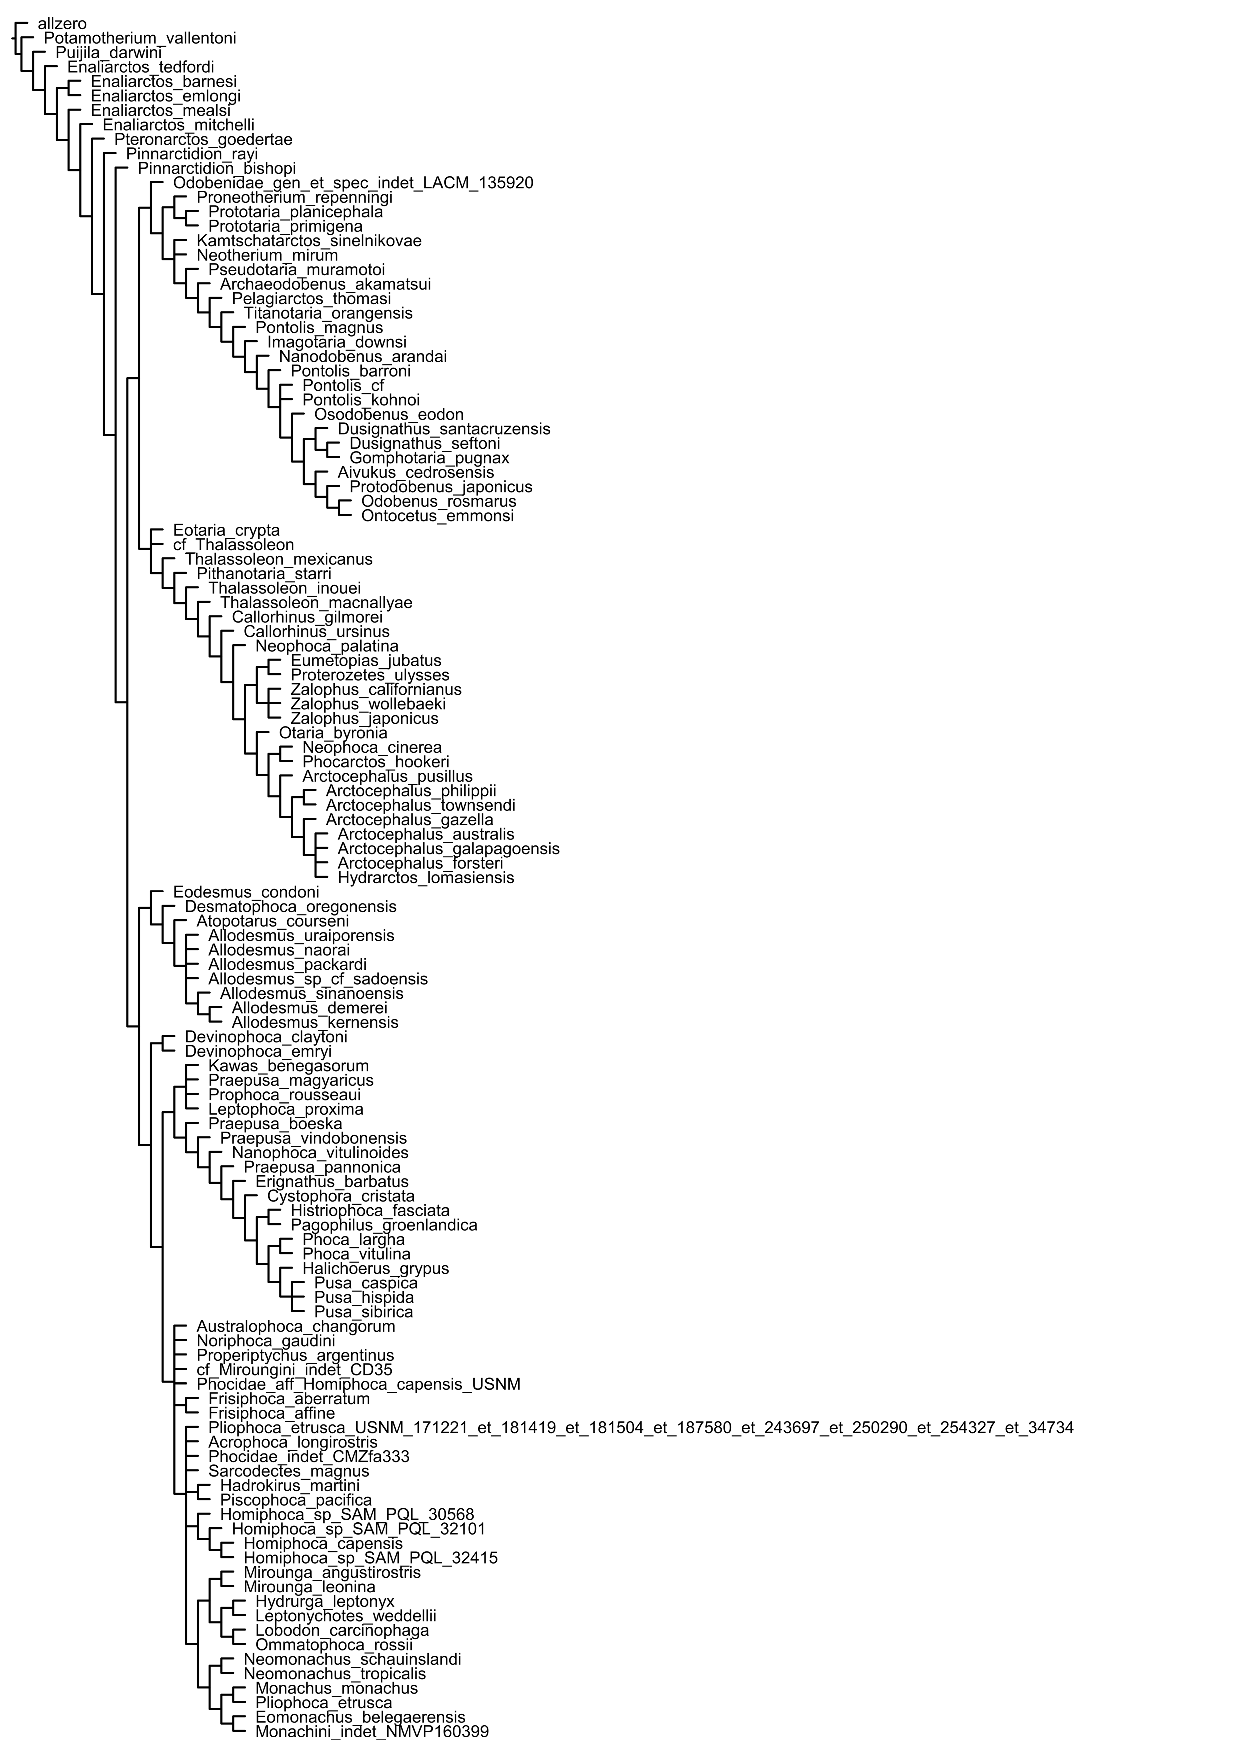
\includegraphics[width = \linewidth]{figures/STR_SCC.pdf}
  \caption{Strict consensus topology.}
  \label{fig-sc}
\end{figure}

\subsubsection{Majority rule consensus topology}

This topology is shown in Figure \ref{fig-mrc}. All major pinniped clades were recovered as monophyletic (Desmatophocidae, Odobenidae, Otariidae, Phocidae). Otarioidea and Phocoidea were also recovered. In stem pan-pinnipeds, both \textit{Enaliarctos} and \textit{Pinnarctidion} are paraphyletic. The topology is identical to that of the median tree apart from the taxa removed during time-scaling and the following exceptions: \textit{Pliopedia} forms a polytomy with \textit{Protodobenus} and all other more crown-ward odobenids; \textit{Eotaria} spp. and cf. \textit{Thalassoleon} form a polytomy with all other otariids at the base of the clade, rather than \textit{Eotaria} diverging before cf. \textit{Thalassoleon}; \textit{Allodesmus uraiporensis} forms a polytomy with (\textit{A.} sp. cf. \textit{sadoensis} $+$ \textit{A. naroai}) $+$ (\textit{A. sinaoensis} $+$ (\textit{A. kernensis} $+$ \textit{A. demerei})).

% figure
\begin{figure}[H]
  \centering
  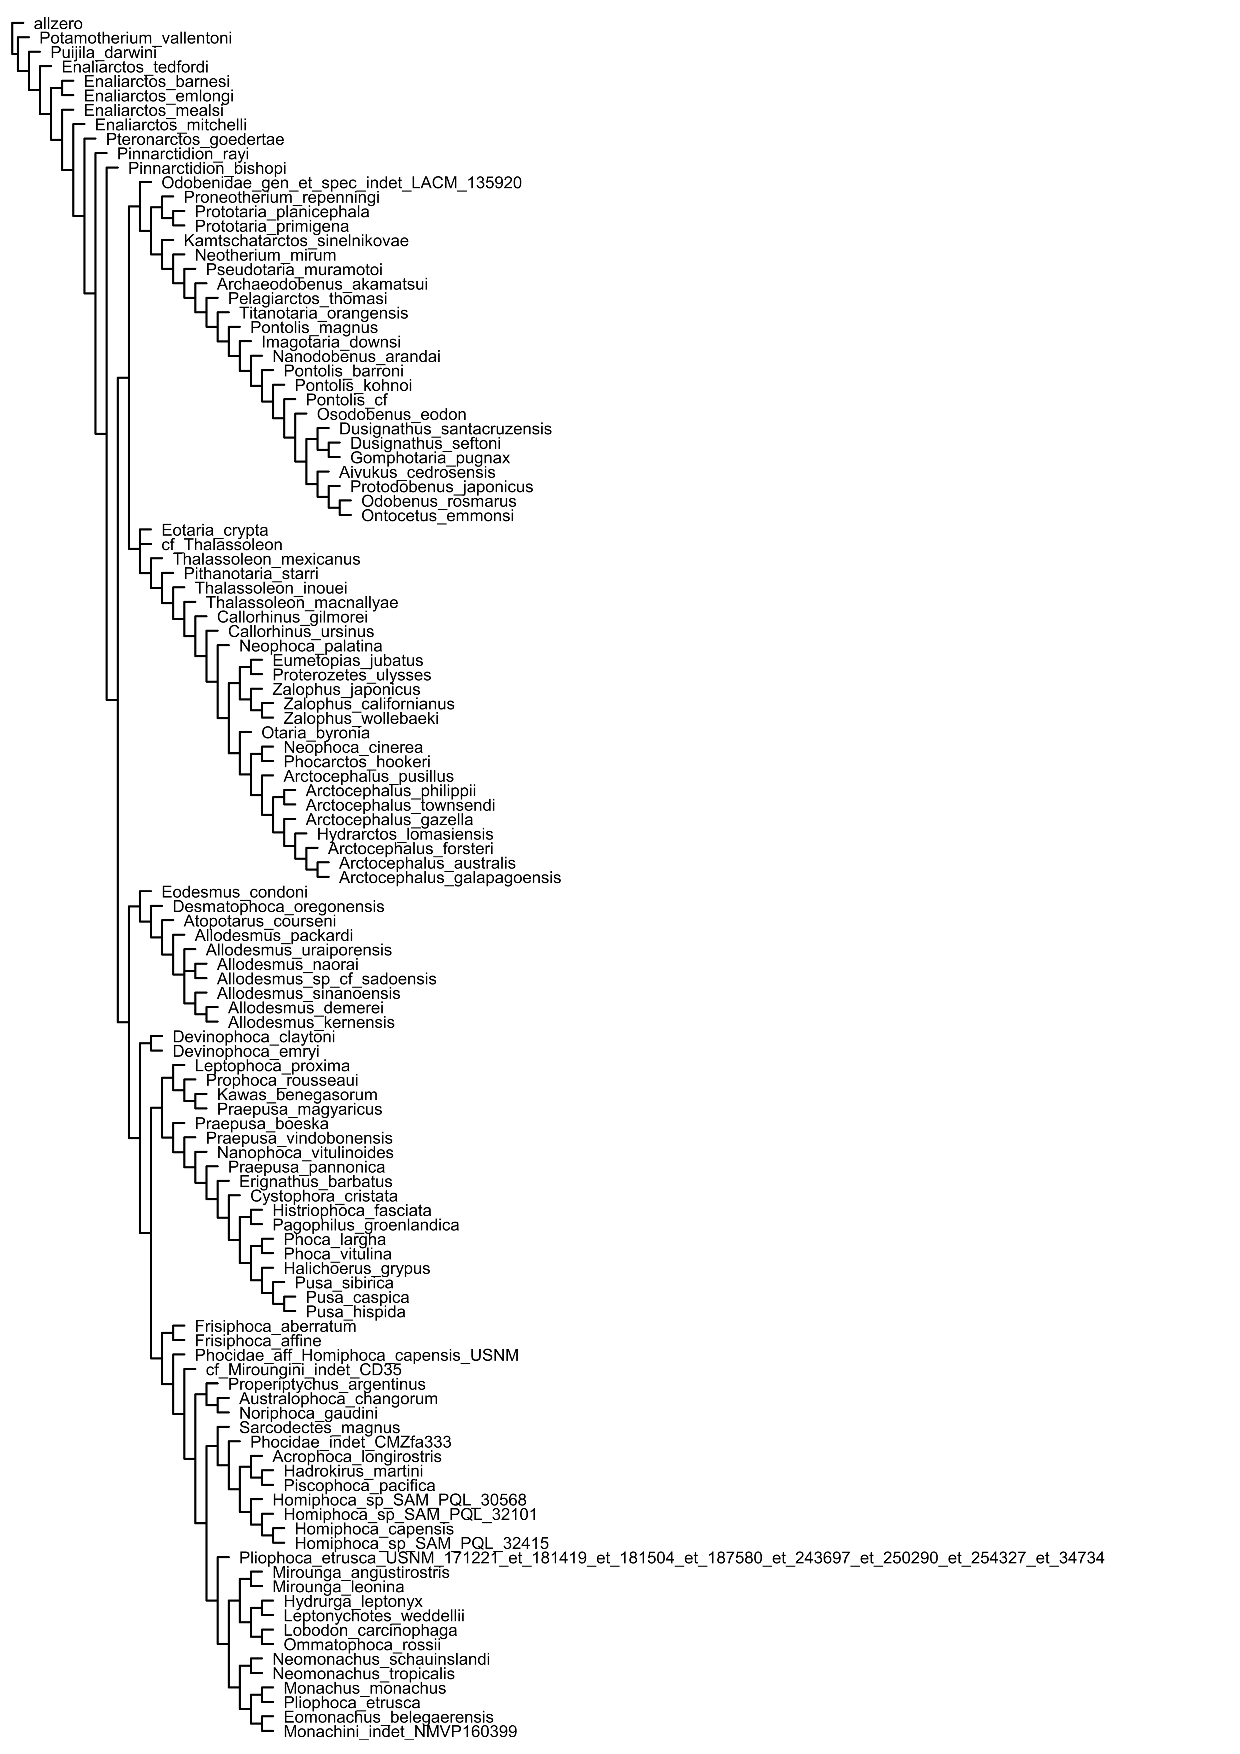
\includegraphics[width = \linewidth]{figures/STR_MRC.pdf}
  \caption{Majority rule consensus topology.}
  \label{fig-mrc}
\end{figure}

\subsection{Extended discussion}

%-------------------------------------------------------------------------------
% Diversification
%-----------------------------------------------------------------------------------
\newpage
\section{Diversification dynamics}

The plots below show the results from the fossilBAMM sensitivity analyses. 
Taxon names have been removed from Figures \ref{fig-noanc-0-01}-\ref{fig-full-10} for readability.

\subsection{Excluding sampled ancestors}

\subsubsection{$\lambda_{prior} = 0.01$}

% figure
\begin{figure}[H]
  \centering
  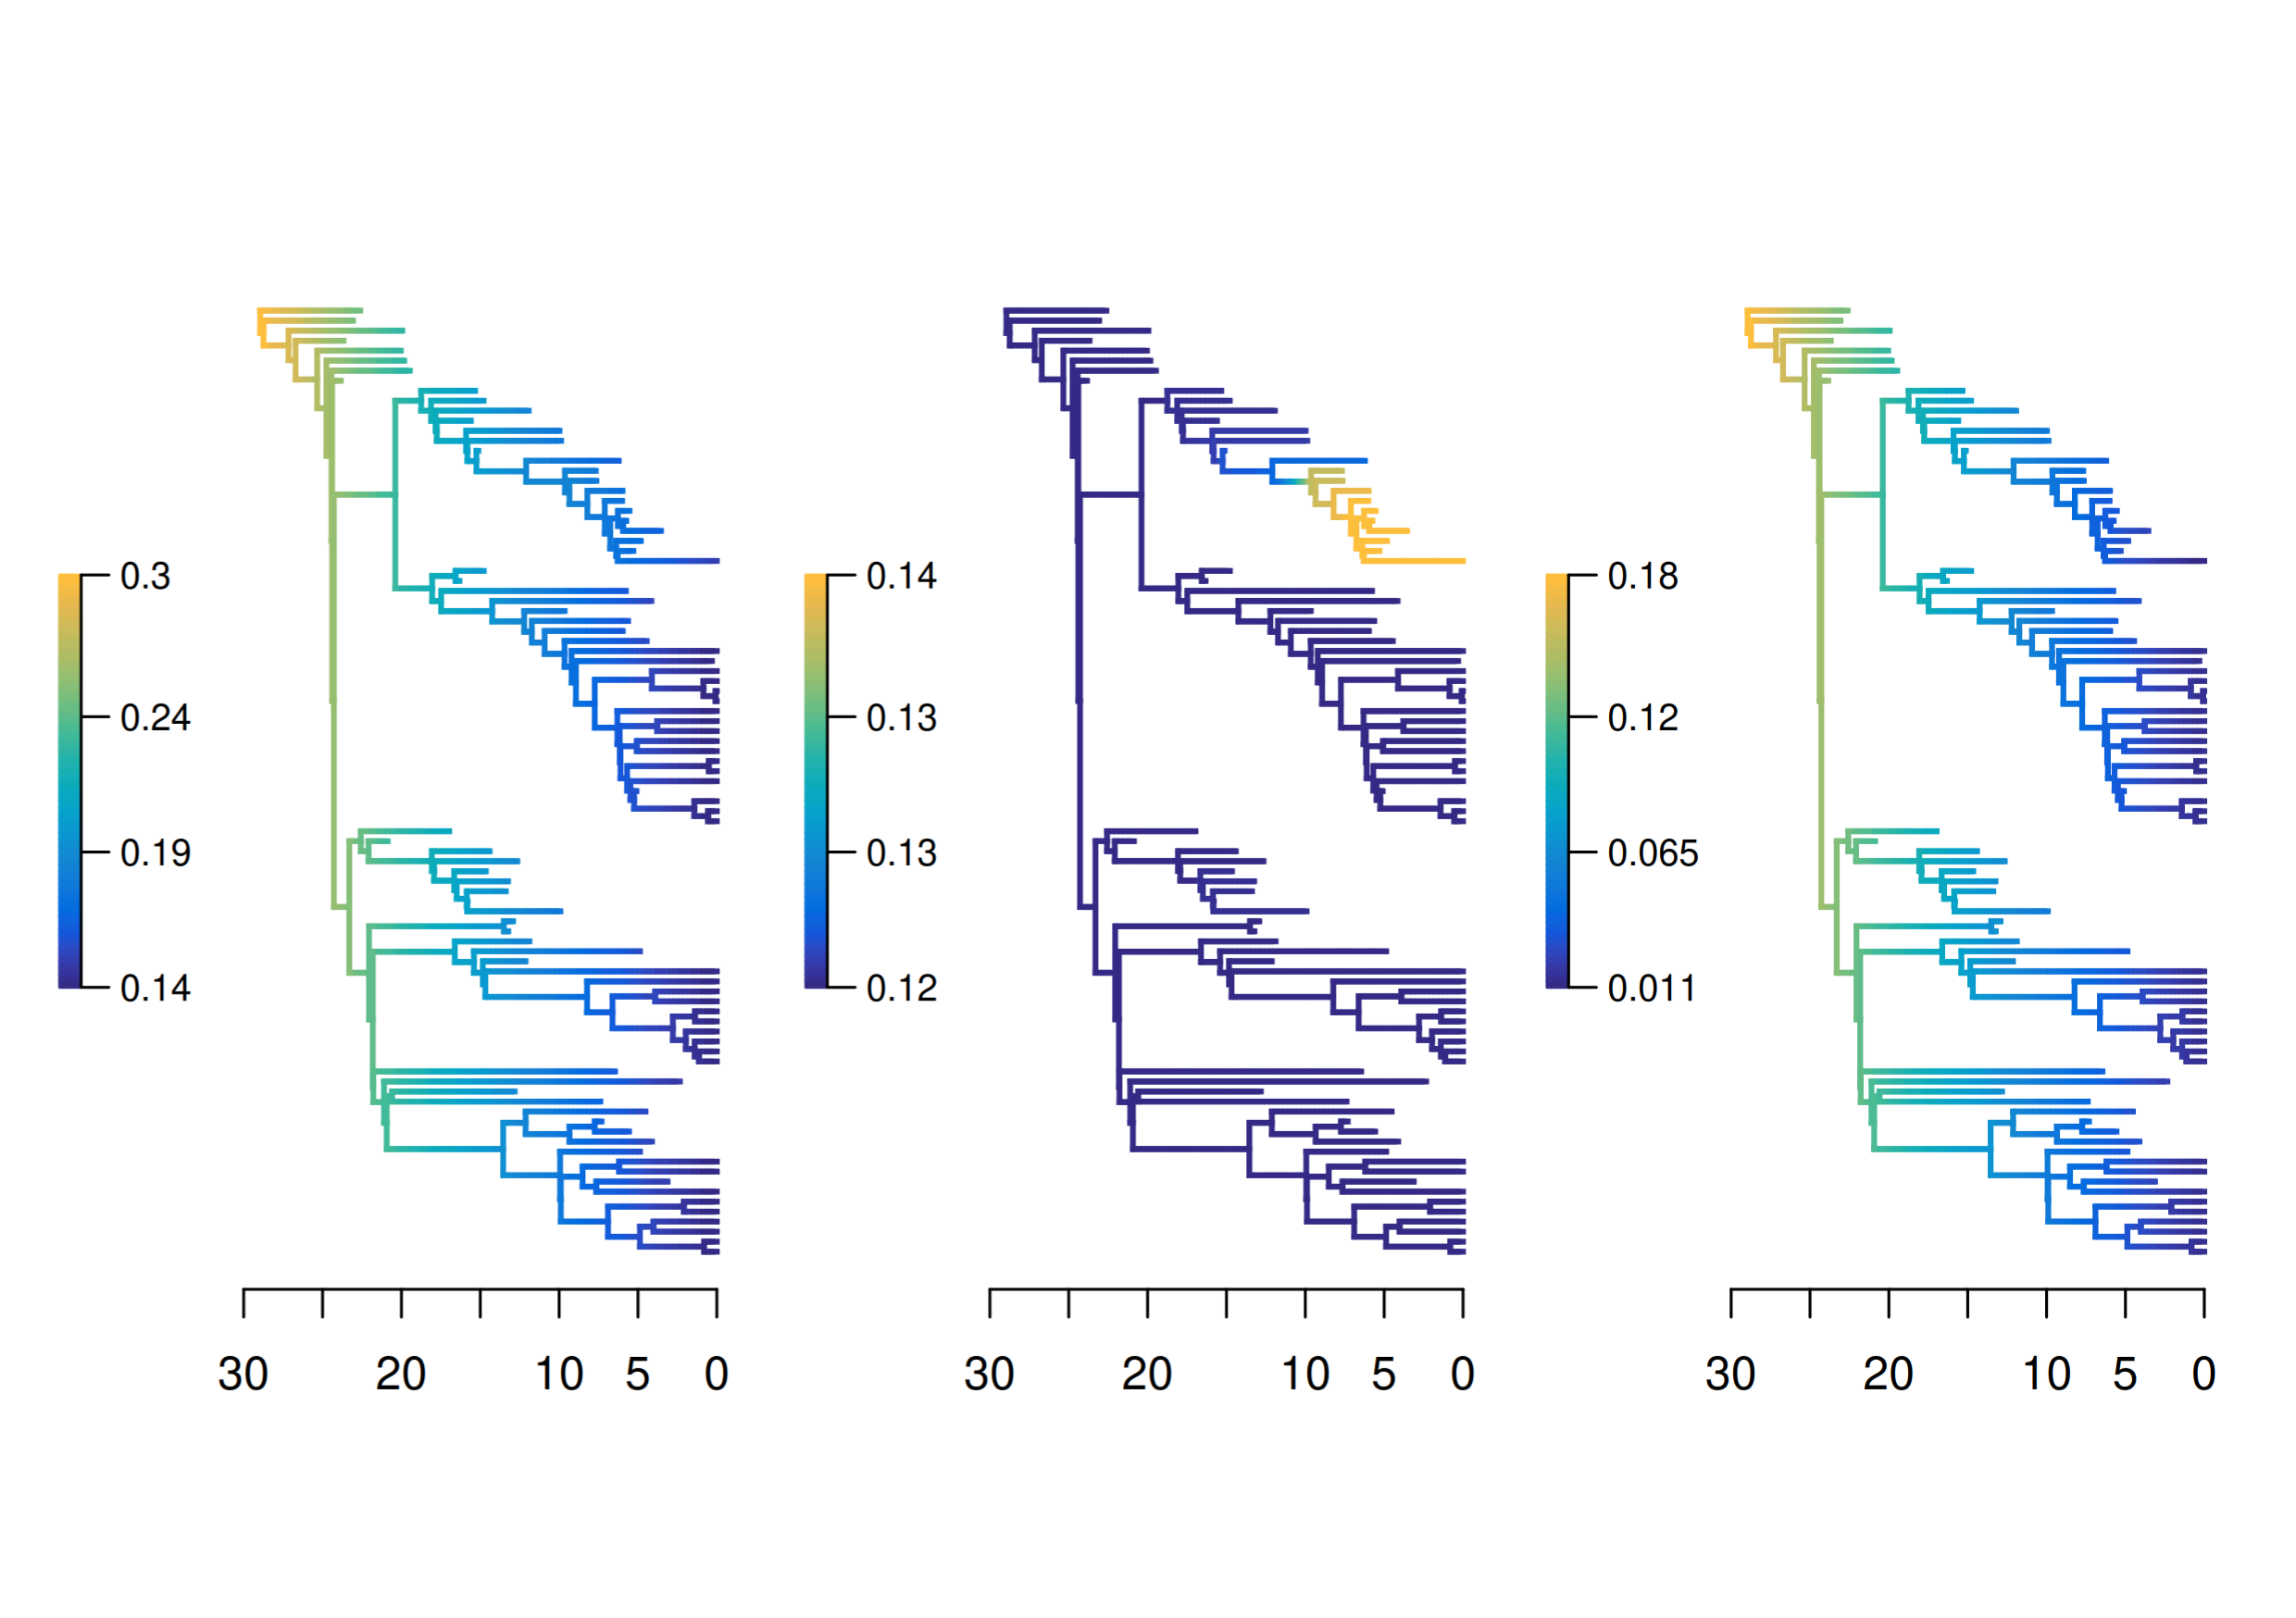
\includegraphics[width = \linewidth]{figures/diversification/sensitivity-analyses/shifts-0-01/sensitivity-analysis-noanc-0-01.png}
  \caption{Excluding sampled ancestors. $\lambda_{prior} = 0.01$. Left, middle and right panels indicate speciation, extinction and net diversification rates, respectively.}
  \label{fig-noanc-0-01}
\end{figure}

\subsubsection{$\lambda_{prior} = 0.1$}

% figure
\begin{figure}[H]
  \centering
  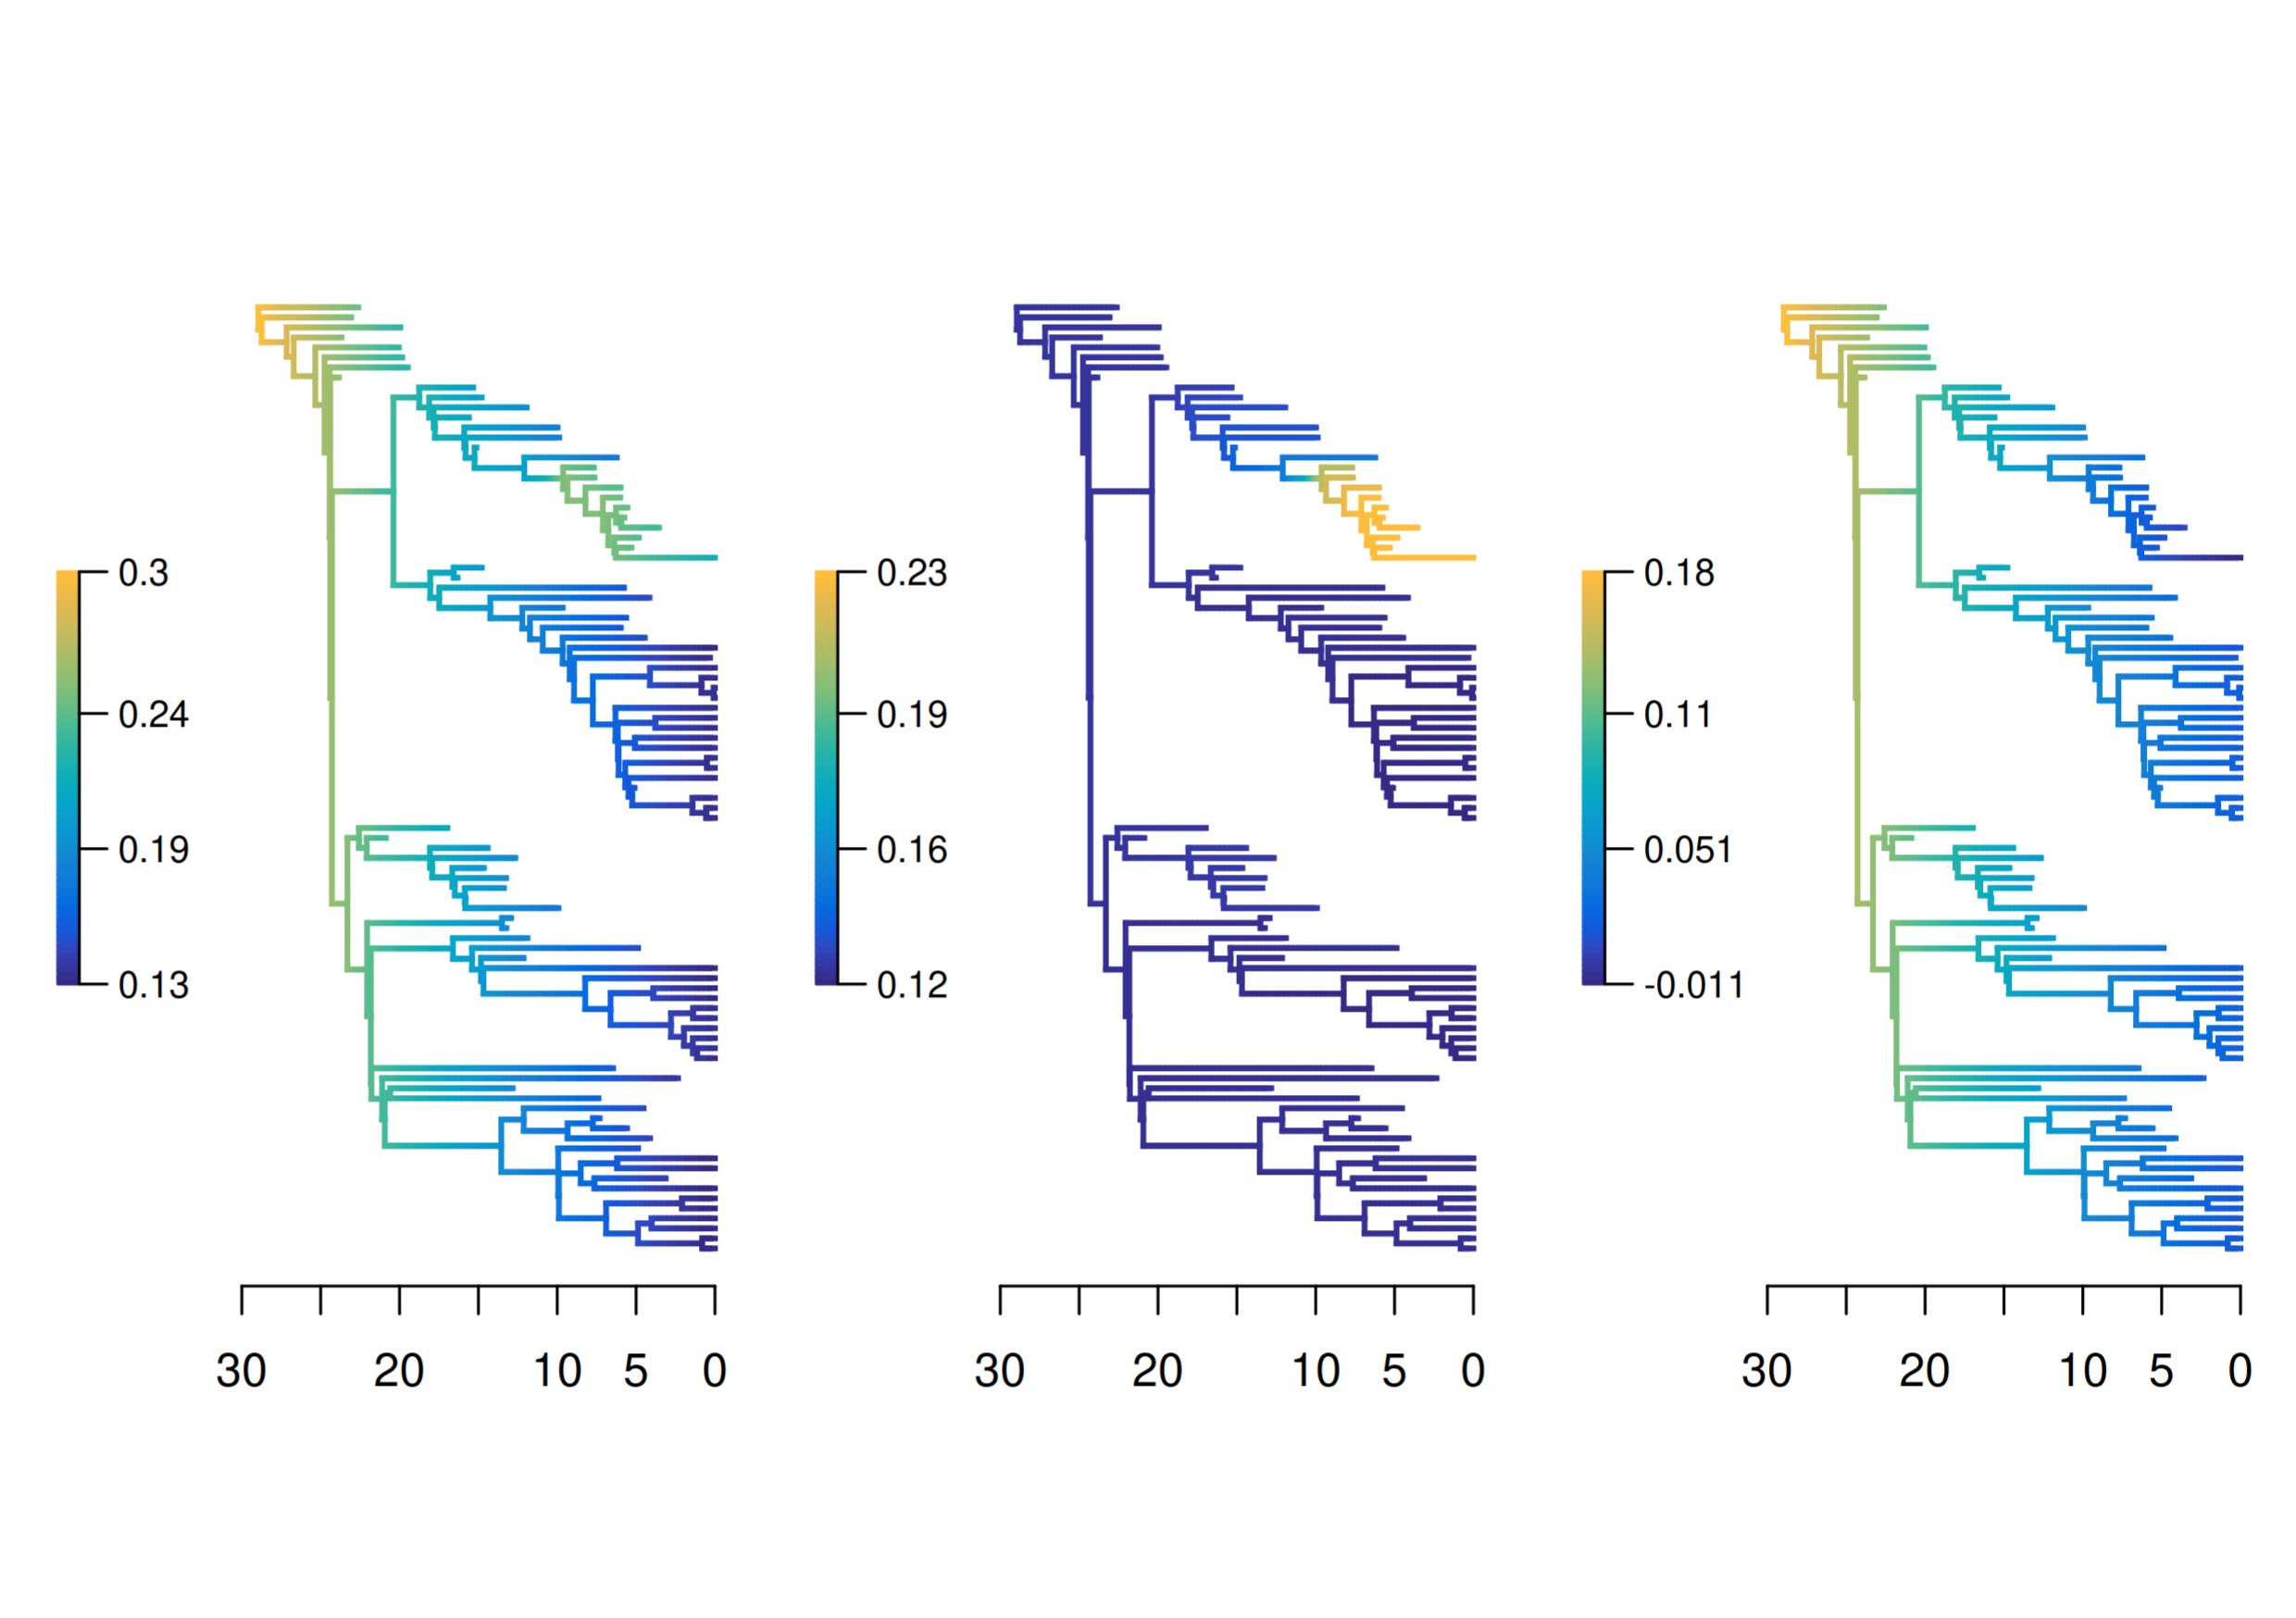
\includegraphics[width = \linewidth]{figures/diversification/sensitivity-analyses/shifts-0-1/sensitivity-analysis-noanc-0-1.png}
  \caption{Excluding sampled ancestors. $\lambda_{prior} = 0.1$. Left, middle and right panels indicate speciation, extinction and net diversification rates, respectively.}
  \label{fig-noanc-0-1}
\end{figure}

\subsubsection{$\lambda_{prior} = 0.5$}

% figure
\begin{figure}[H]
  \centering
  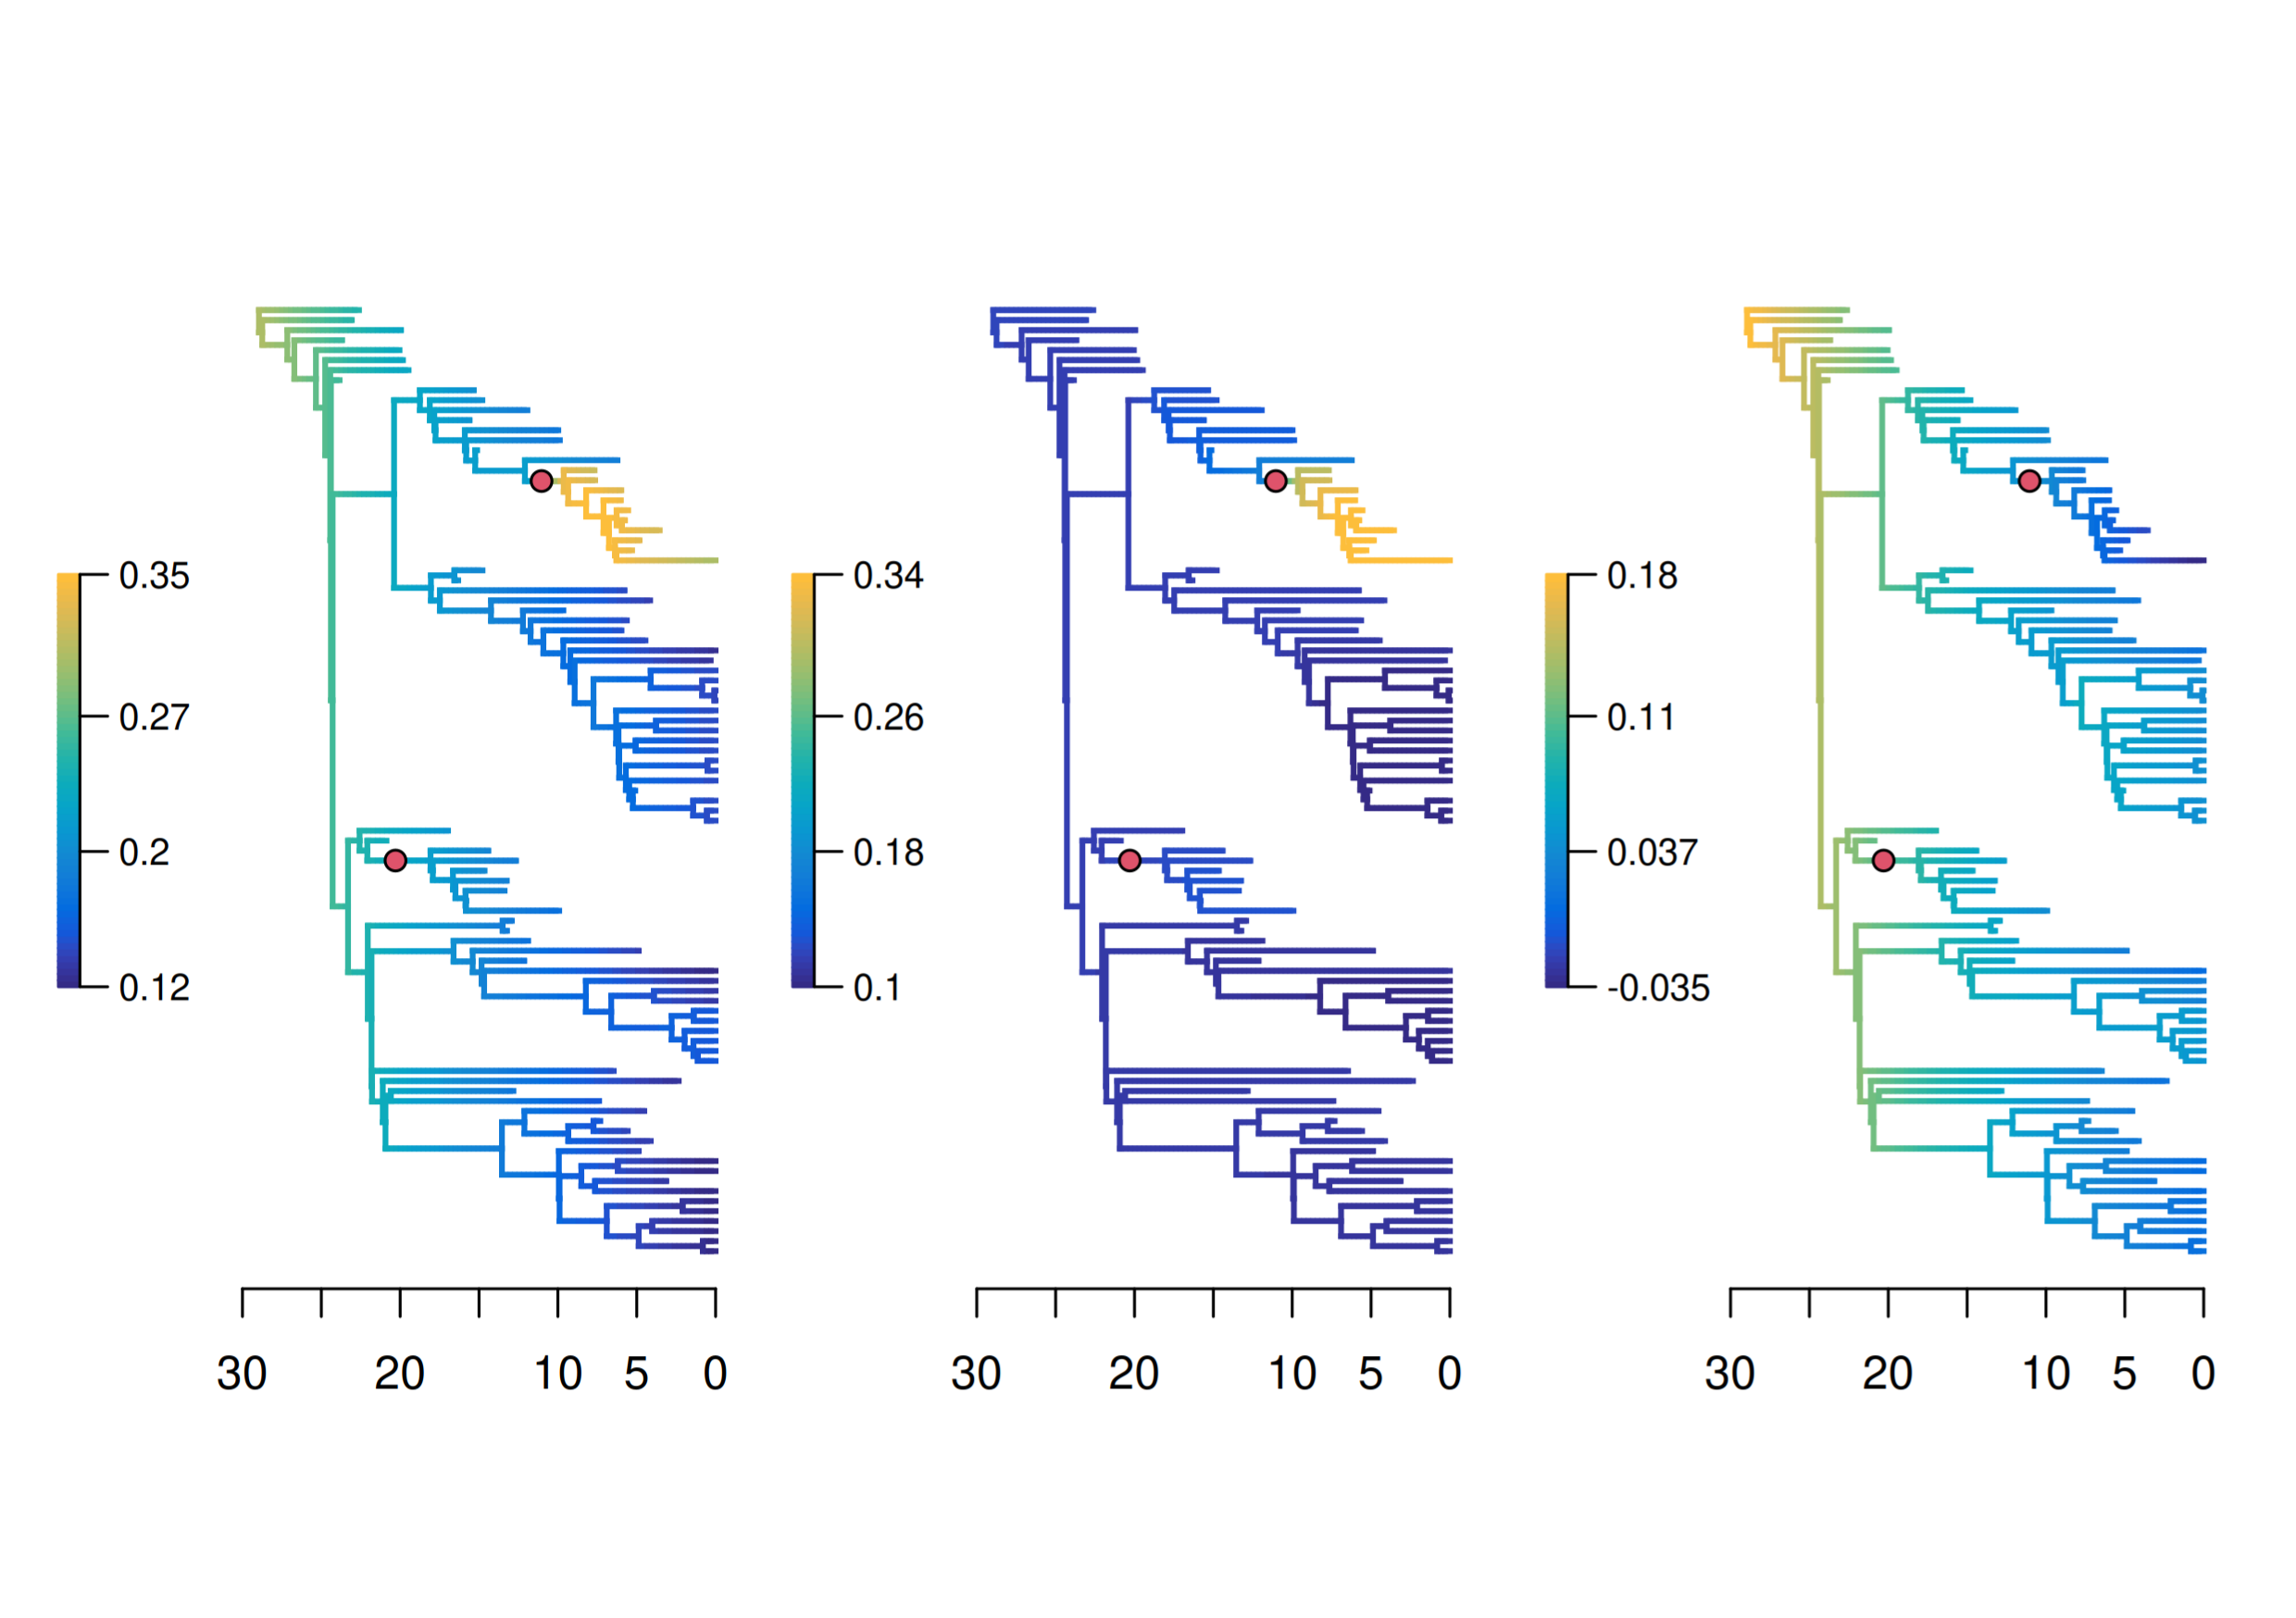
\includegraphics[width = \linewidth]{figures/diversification/sensitivity-analyses/shifts-0-5/sensitivity-analysis-noanc-0-5.png}
  \caption{Excluding sampled ancestors. $\lambda_{prior} = 0.5$. Left, middle and right panels indicate speciation, extinction and net diversification rates, respectively.}
  \label{fig-noanc-0-5}
\end{figure}


\subsubsection{$\lambda_{prior} = 2$}

% figure
\begin{figure}[H]
  \centering
  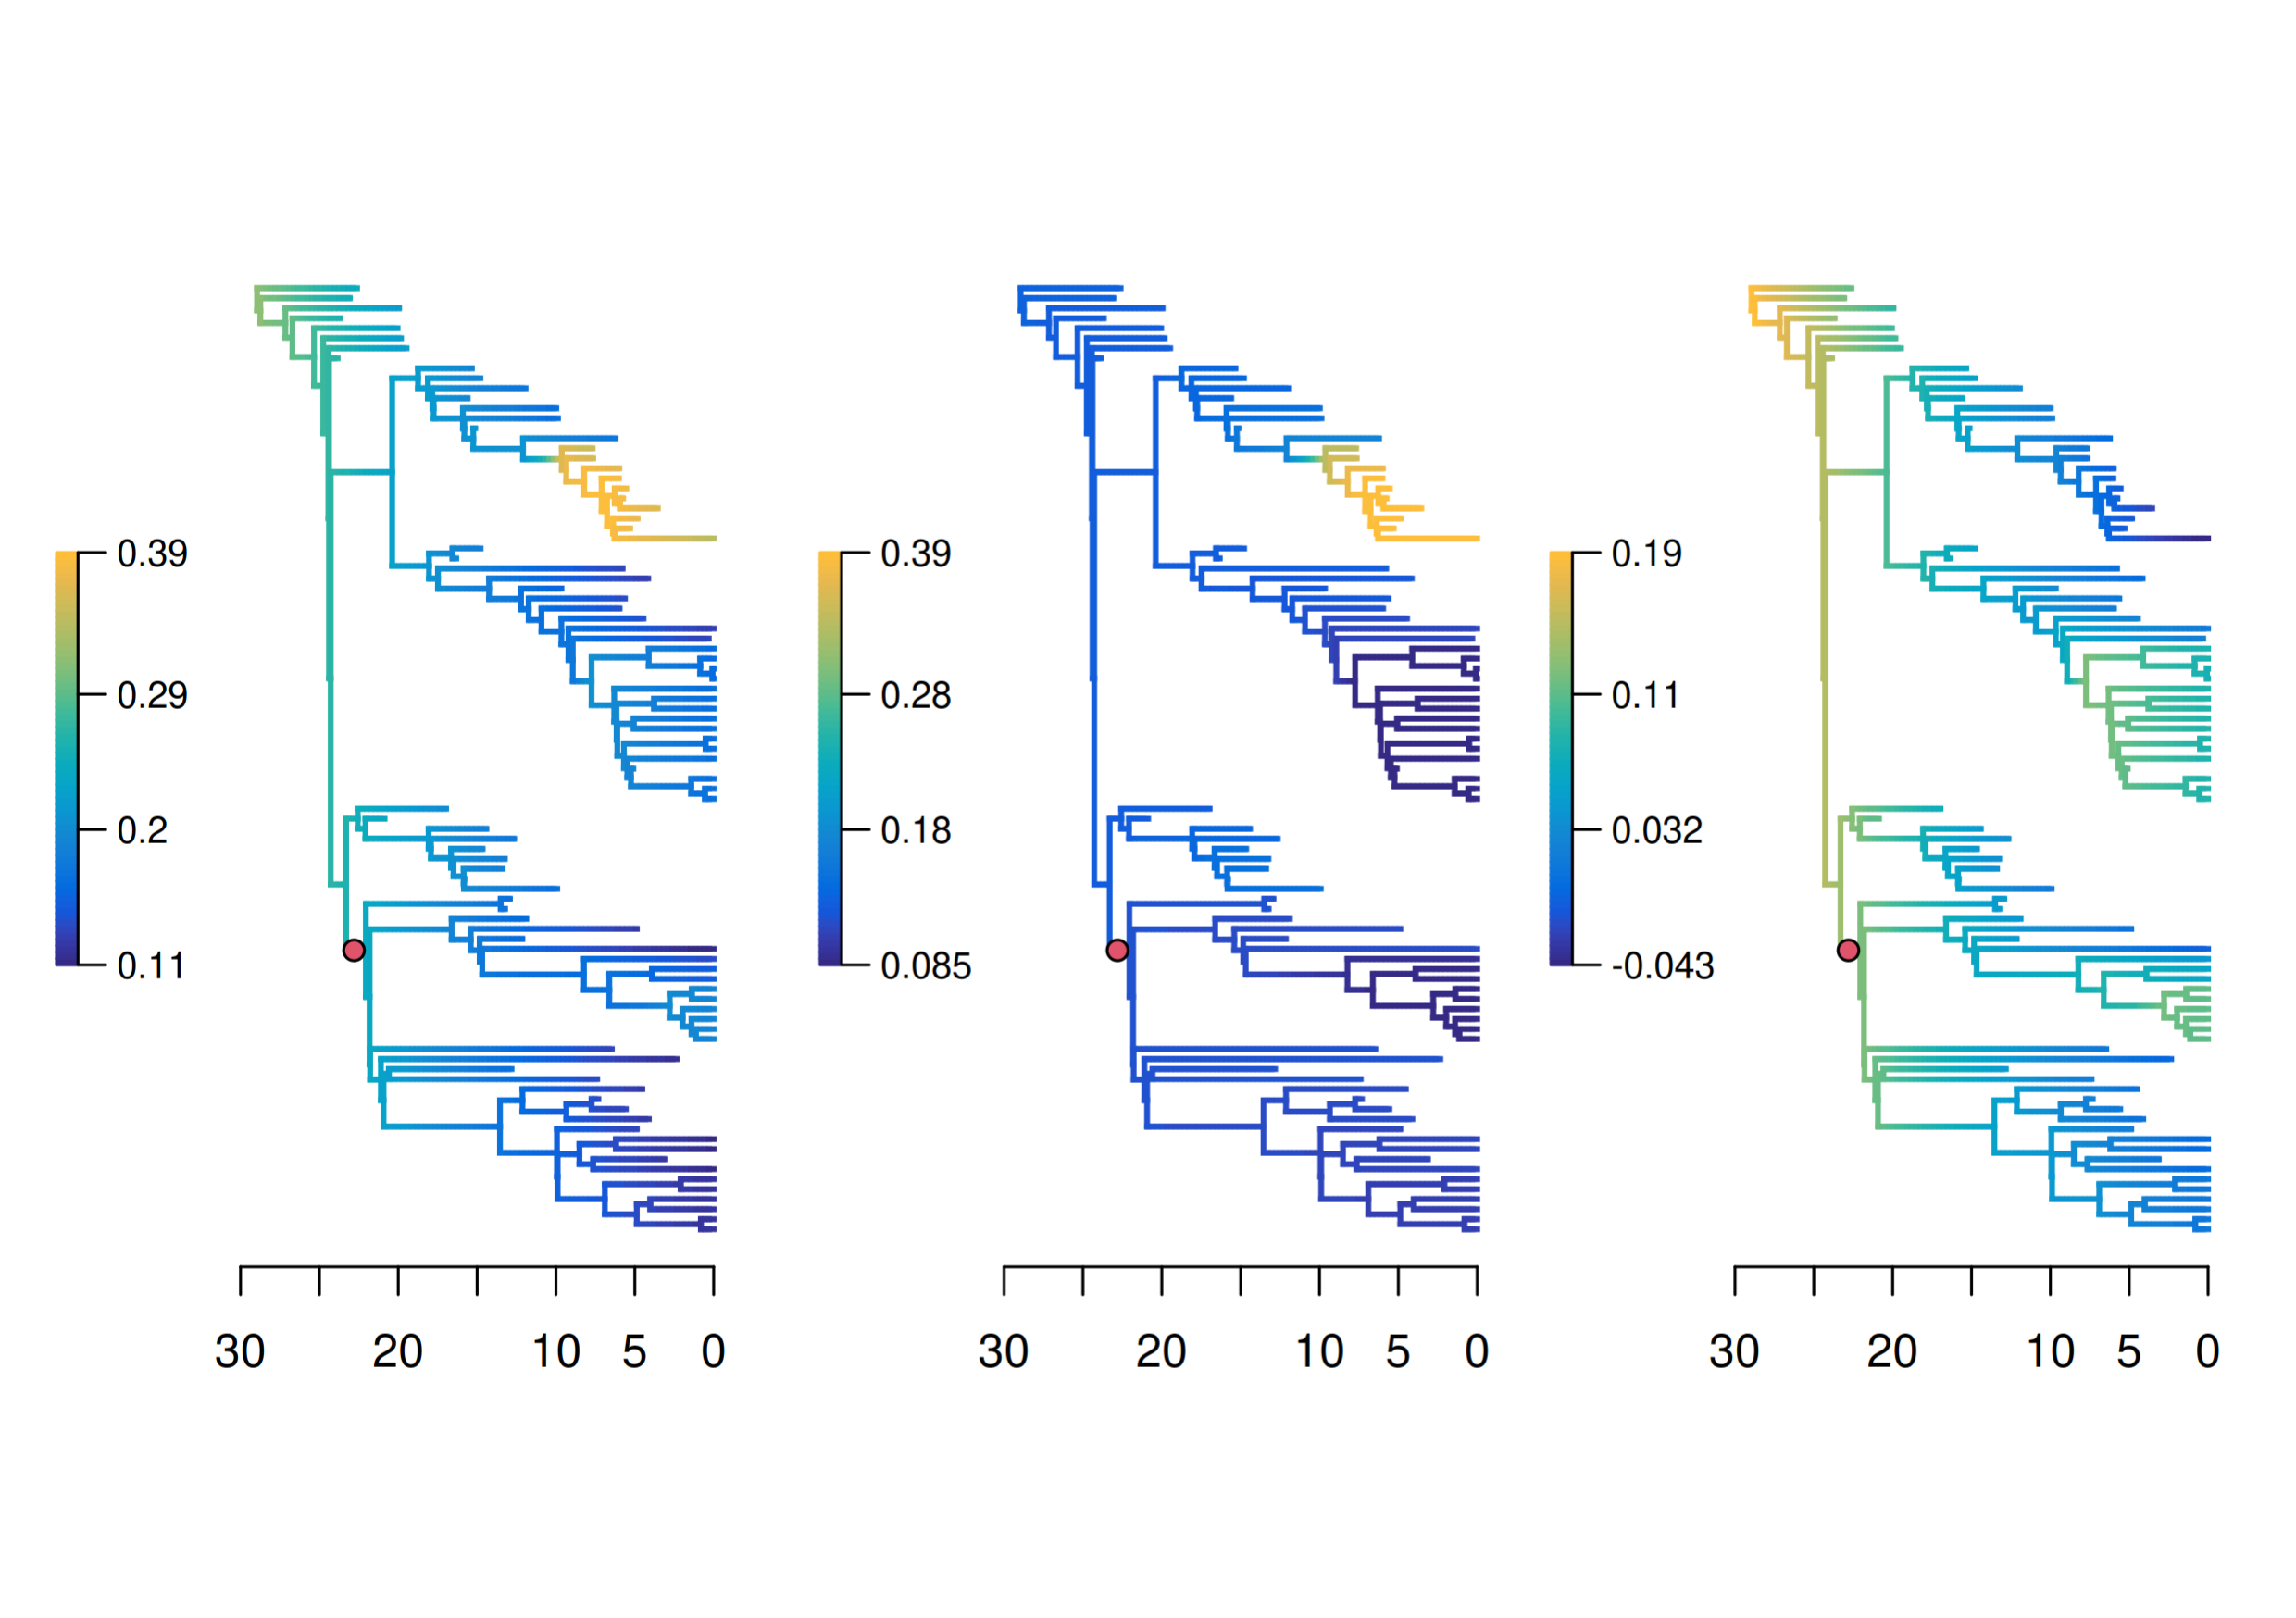
\includegraphics[width = \linewidth]{figures/diversification/sensitivity-analyses/shifts-2/sensitivity-analysis-noanc-2.png}
  \caption{Excluding sampled ancestors. $\lambda_{prior} = 2$. Left, middle and right panels indicate speciation, extinction and net diversification rates, respectively.}
  \label{fig-noanc-2}
\end{figure}

\subsubsection{$\lambda_{prior} = 10$}

% figure
\begin{figure}[H]
  \centering
  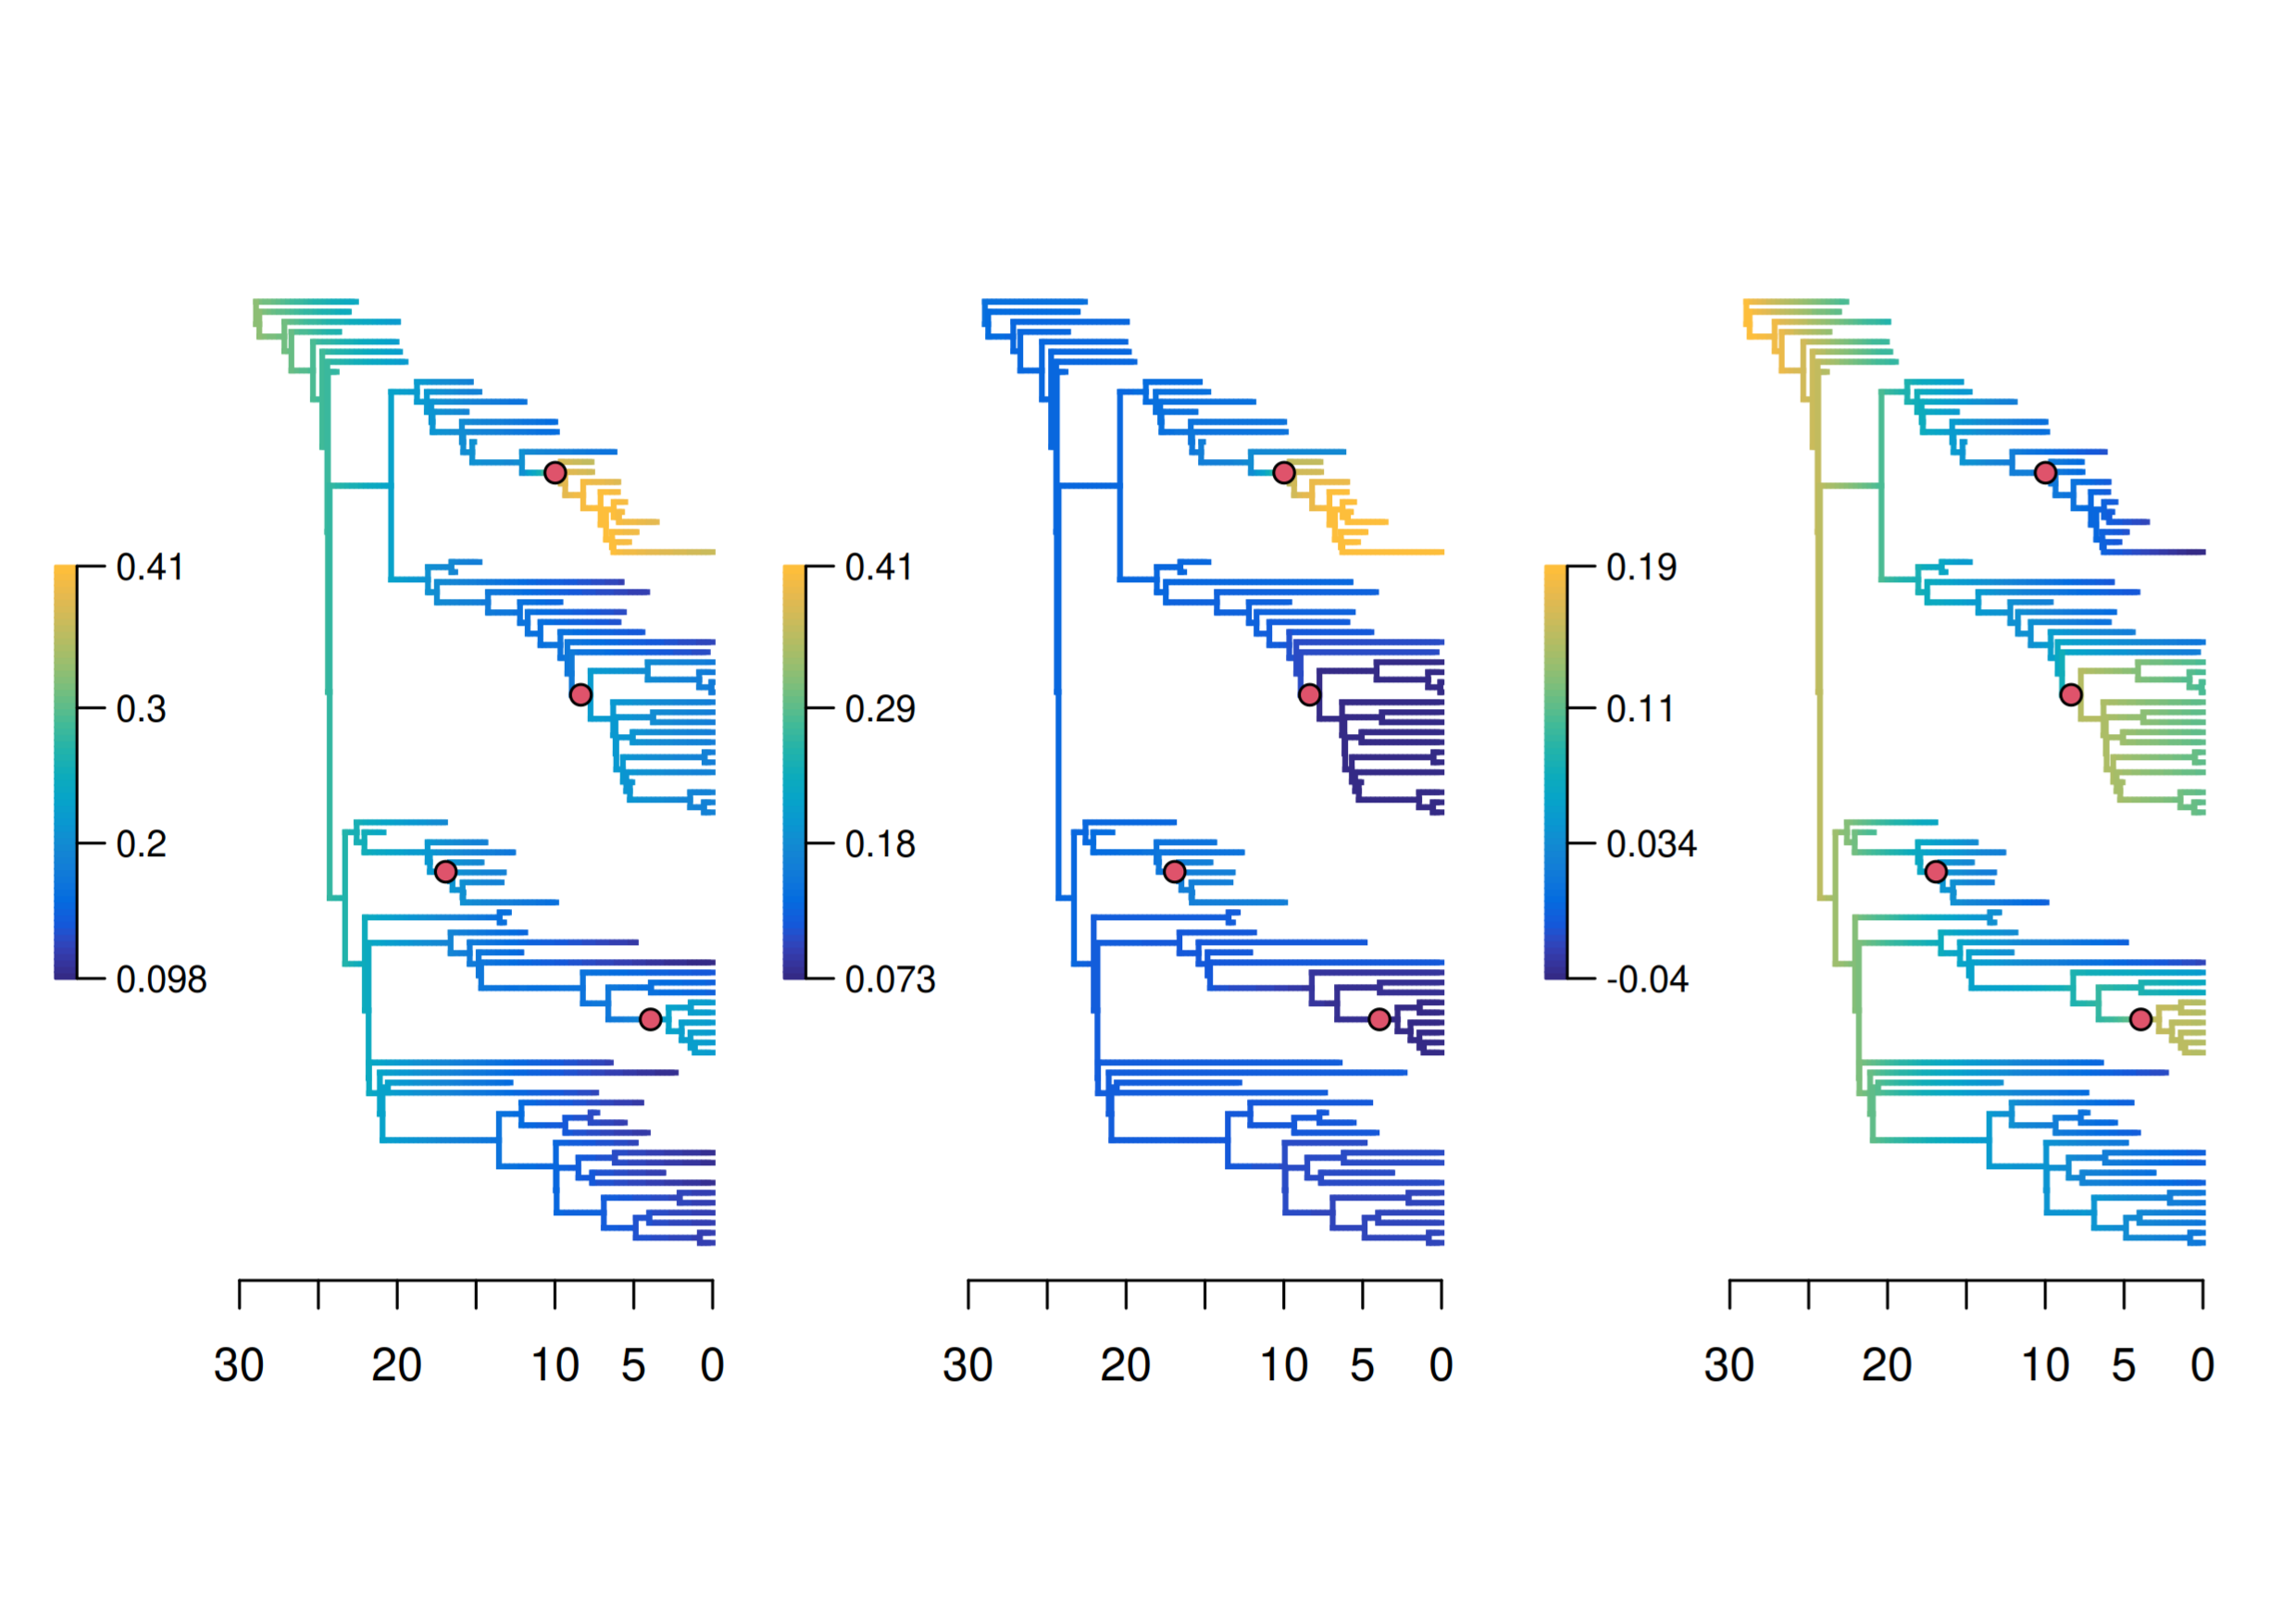
\includegraphics[width = \linewidth]{figures/diversification/sensitivity-analyses/shifts-10/sensitivity-analysis-noanc-10.png}
  \caption{Excluding sampled ancestors. $\lambda_{prior} = 10$. Left, middle and right panels indicate speciation, extinction and net diversification rates, respectively.}
  \label{fig-noanc-10}
\end{figure}

\subsection{Including sampled ancestors}

\subsubsection{$\lambda_{prior} = 0.01$}

% figure
\begin{figure}[H]
  \centering
  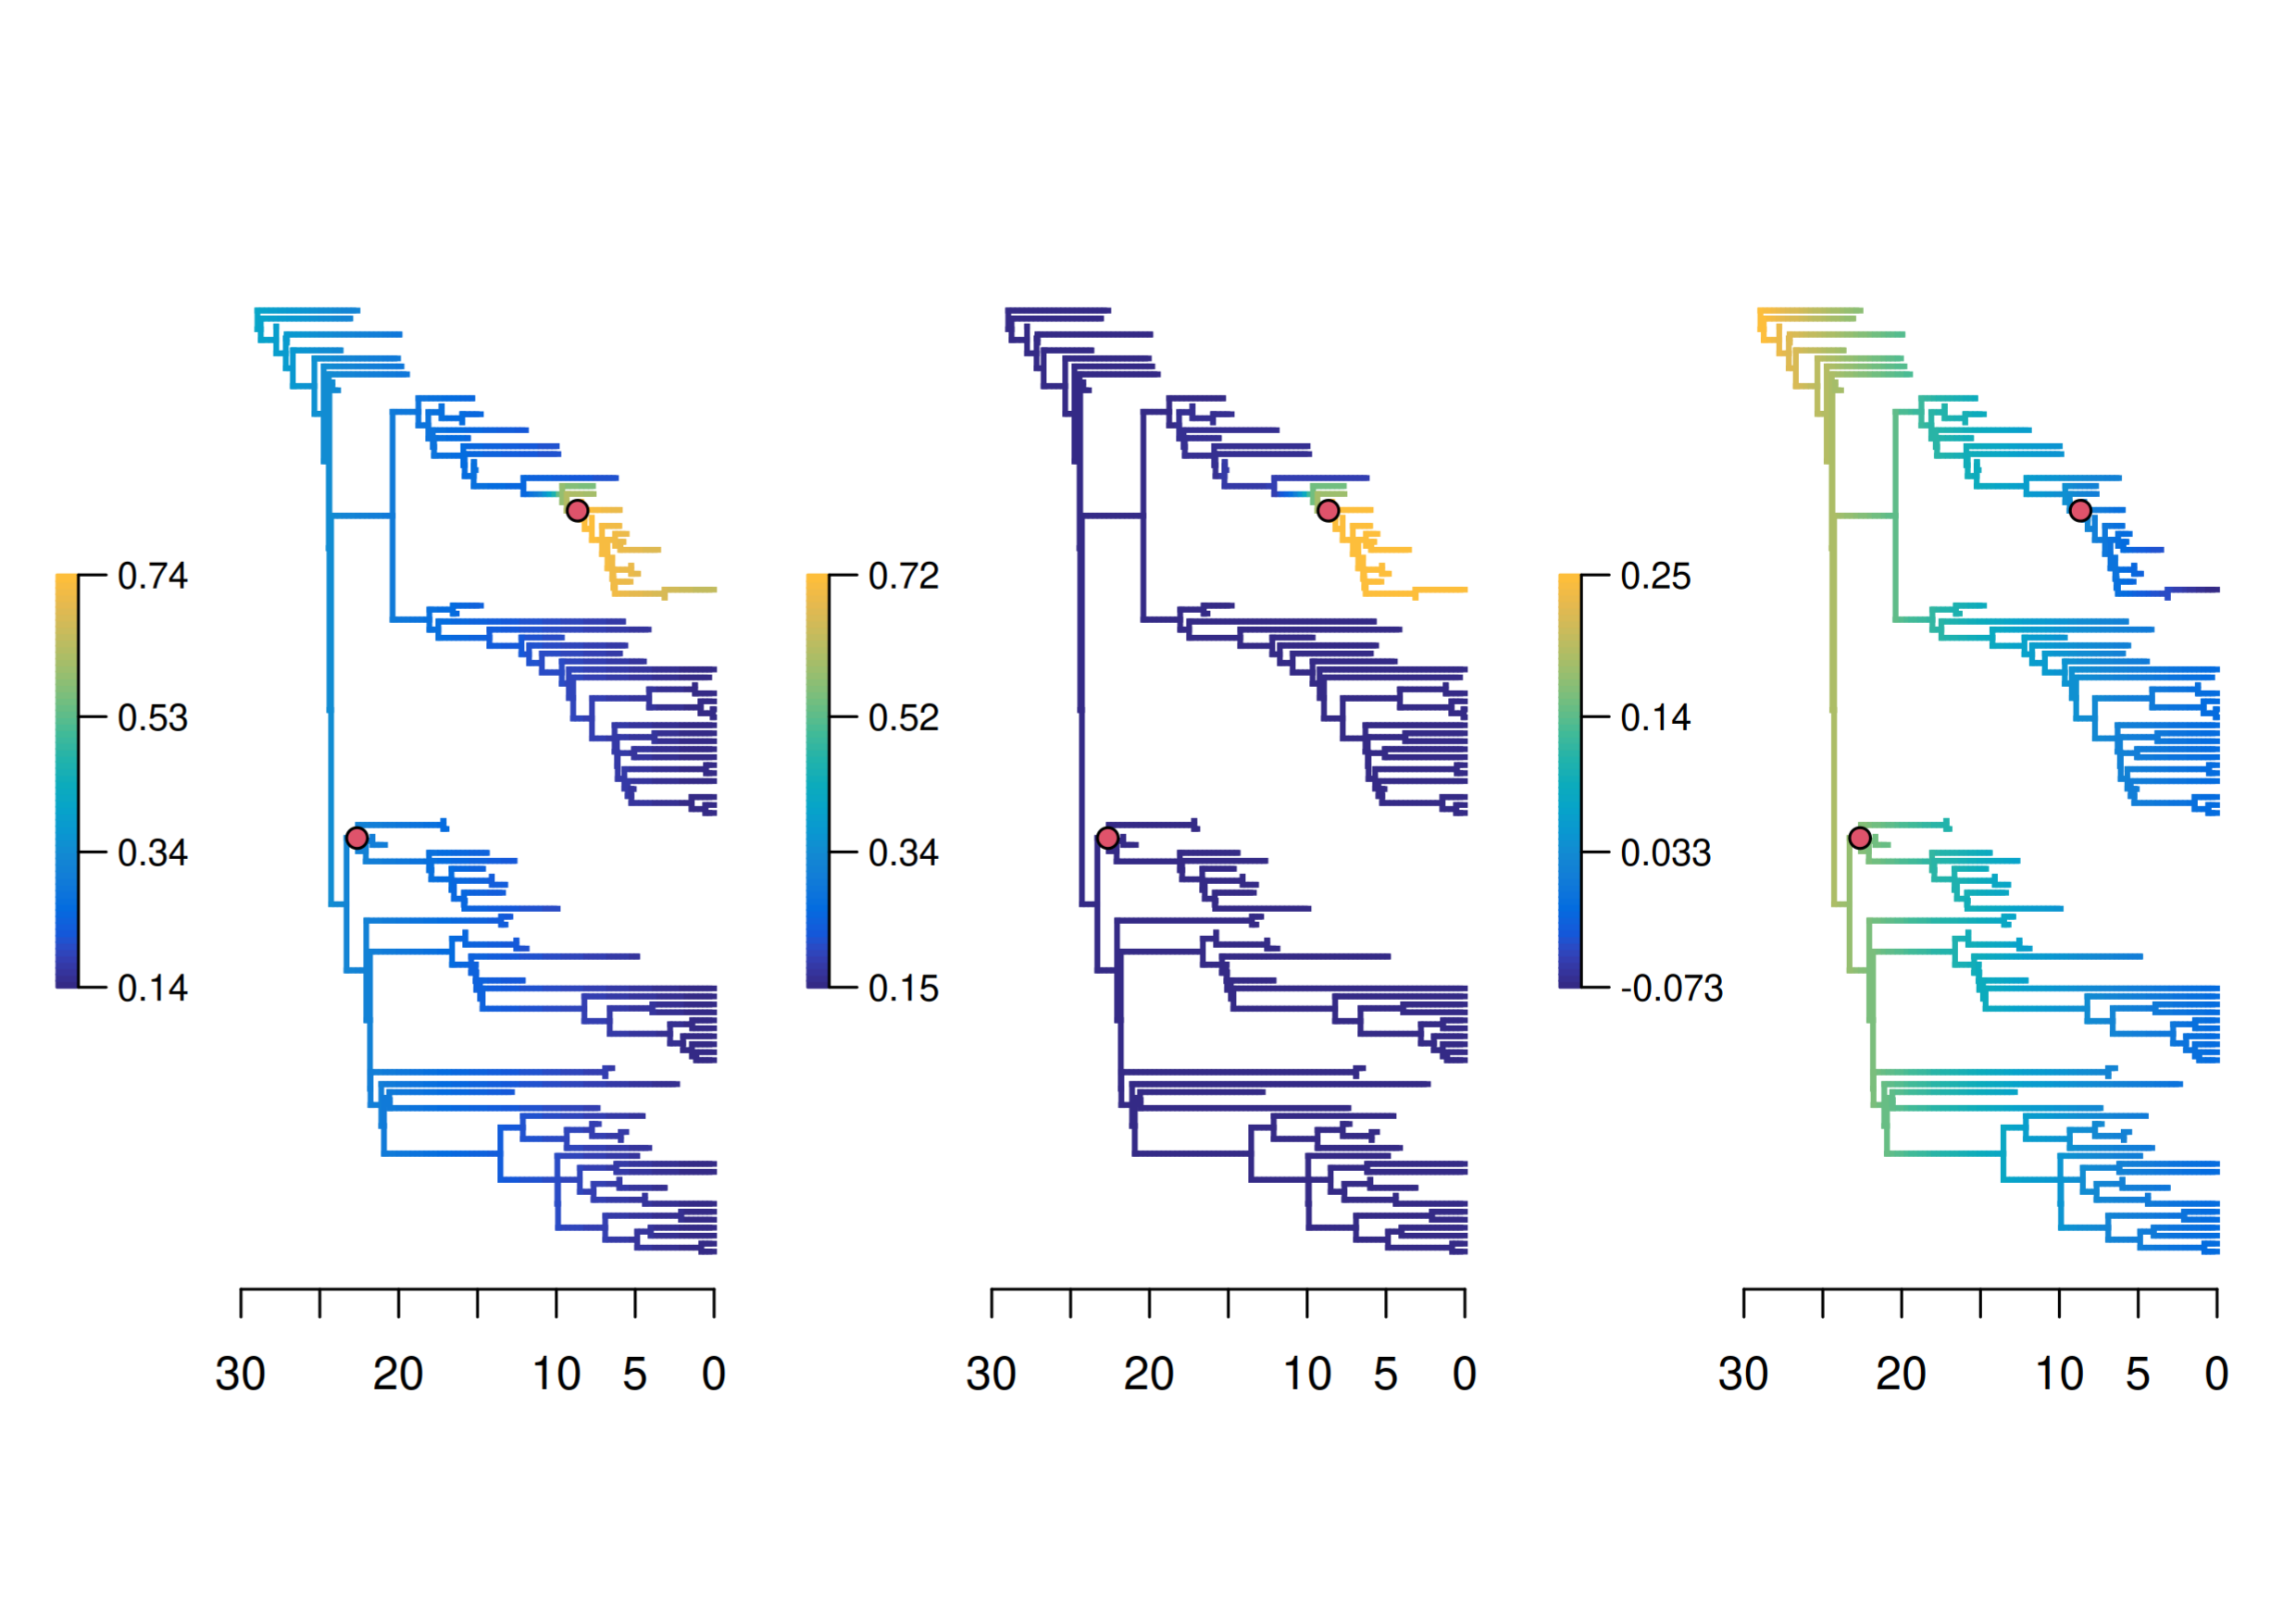
\includegraphics[width = \linewidth]{figures/diversification/sensitivity-analyses-with-sampled-ancestors/shifts-0-01/sensitivity-analysis-with-sampled-ancestors-0-01.png}
  \caption{Including sampled ancestors. $\lambda_{prior} = 0.01$. Left, middle and right panels indicate speciation, extinction and net diversification rates, respectively.}
  \label{fig-full-0-01}
\end{figure}

\subsubsection{$\lambda_{prior} = 0.1$}

% figure
\begin{figure}[H]
  \centering
  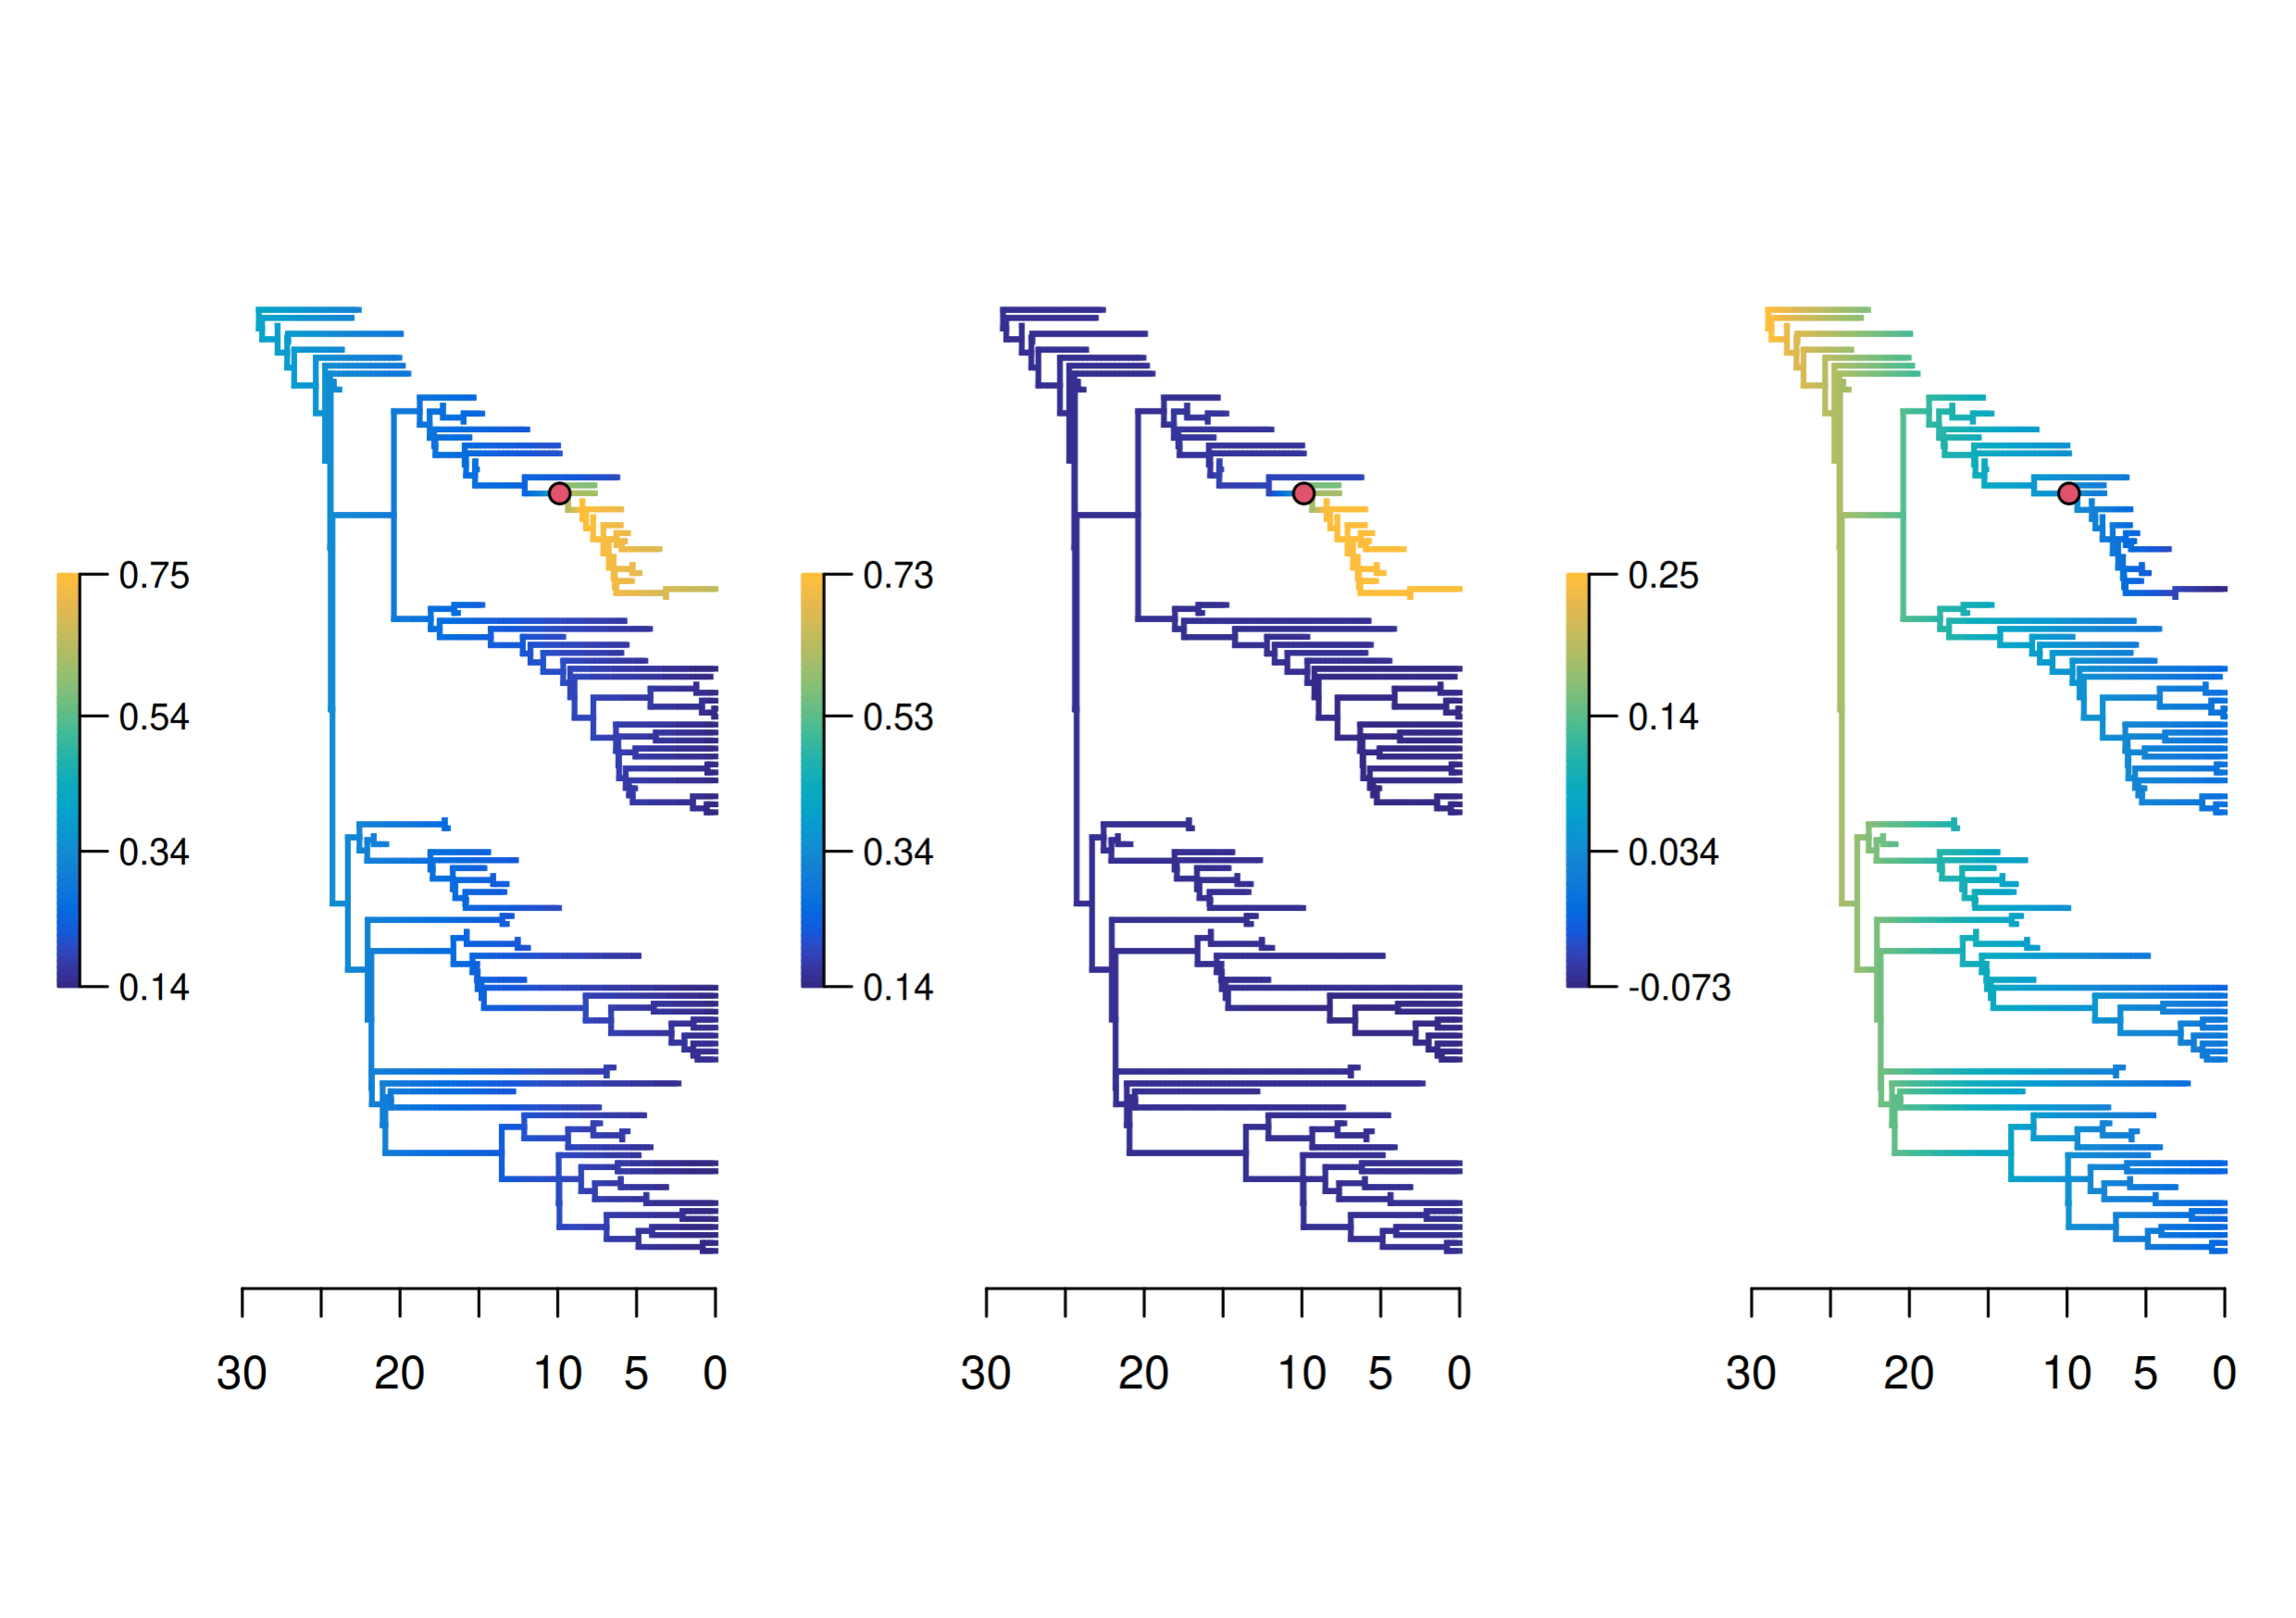
\includegraphics[width = \linewidth]{figures/diversification/sensitivity-analyses-with-sampled-ancestors/shifts-0-1/sensitivity-analysis-with-sampled-ancestors-0-1.png}
  \caption{Including sampled ancestors. $\lambda_{prior} = 0.1$. Left, middle and right panels indicate speciation, extinction and net diversification rates, respectively.}
  \label{fig-full-0-1}
\end{figure}

\subsubsection{$\lambda_{prior} = 0.5$}

% figure
\begin{figure}[H]
  \centering
  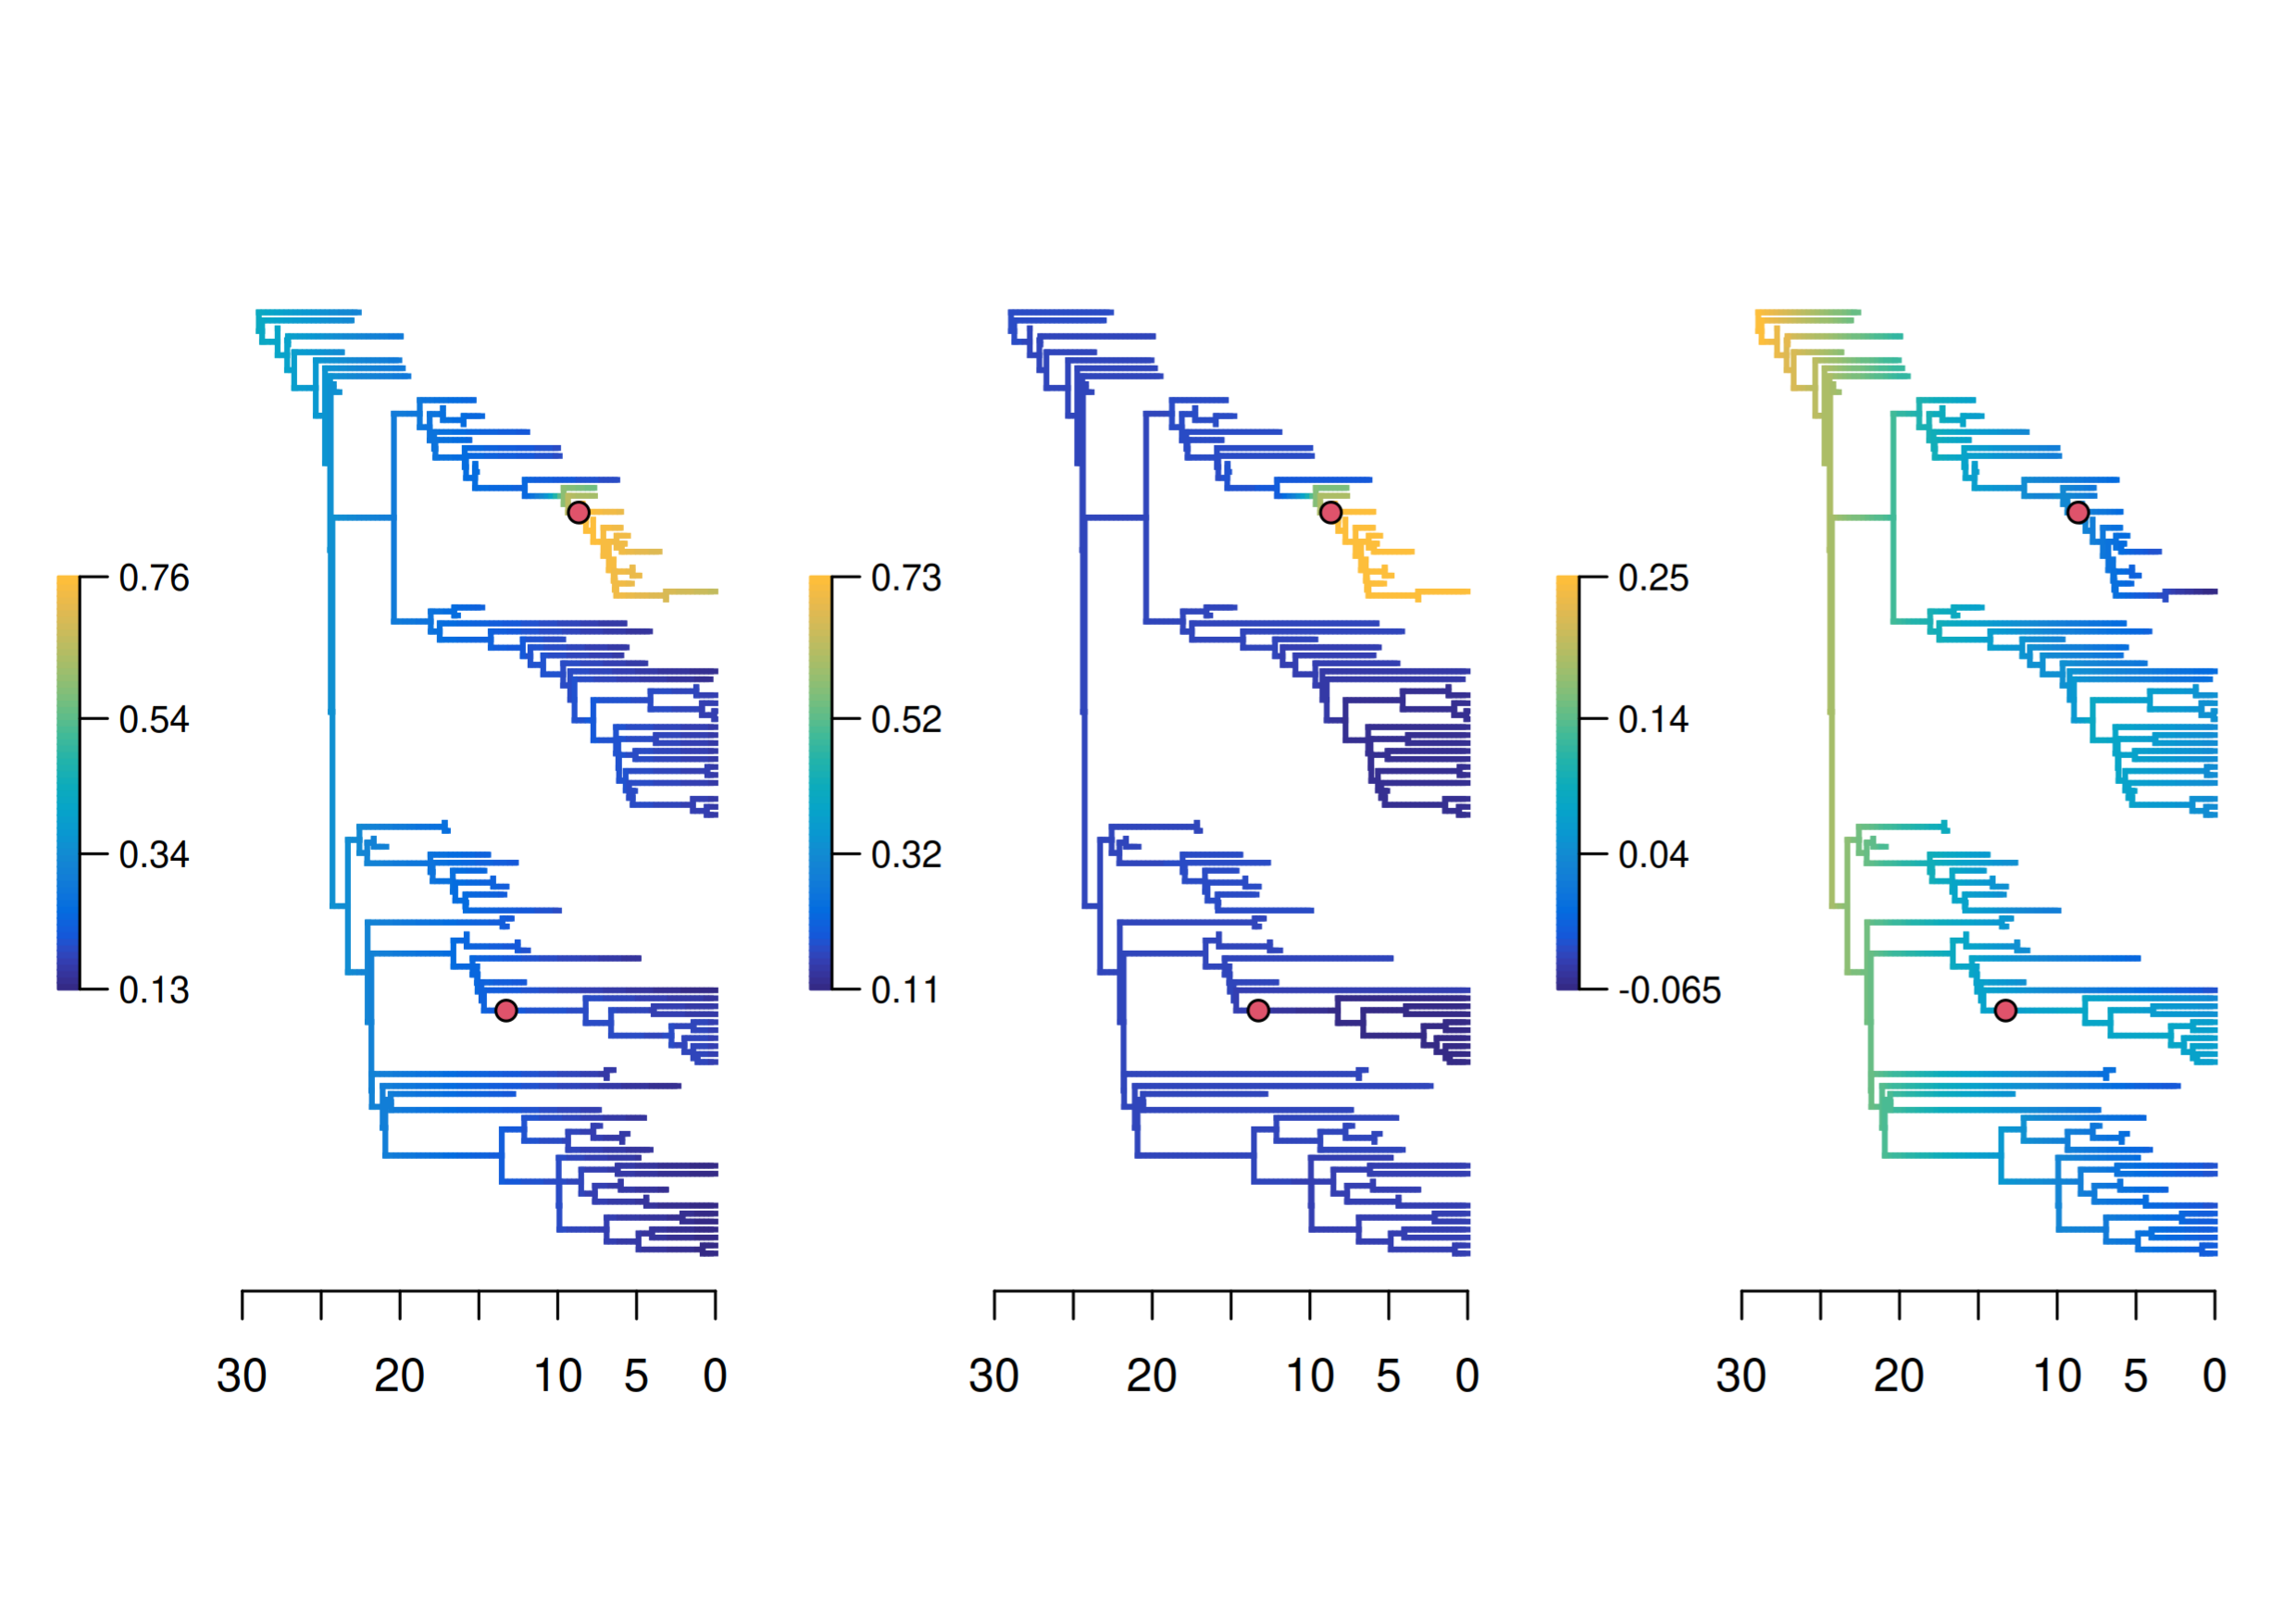
\includegraphics[width = \linewidth]{figures/diversification/sensitivity-analyses-with-sampled-ancestors/shifts-0-5/sensitivity-analysis-with-sampled-ancestors-0-5.png}
  \caption{Including sampled ancestors. $\lambda_{prior} = 0.5$. Left, middle and right panels indicate speciation, extinction and net diversification rates, respectively.}
  \label{fig-full-0-5}
\end{figure}

\subsubsection{$\lambda_{prior} = 1$}

% figure
\begin{figure}[H]
  \centering
  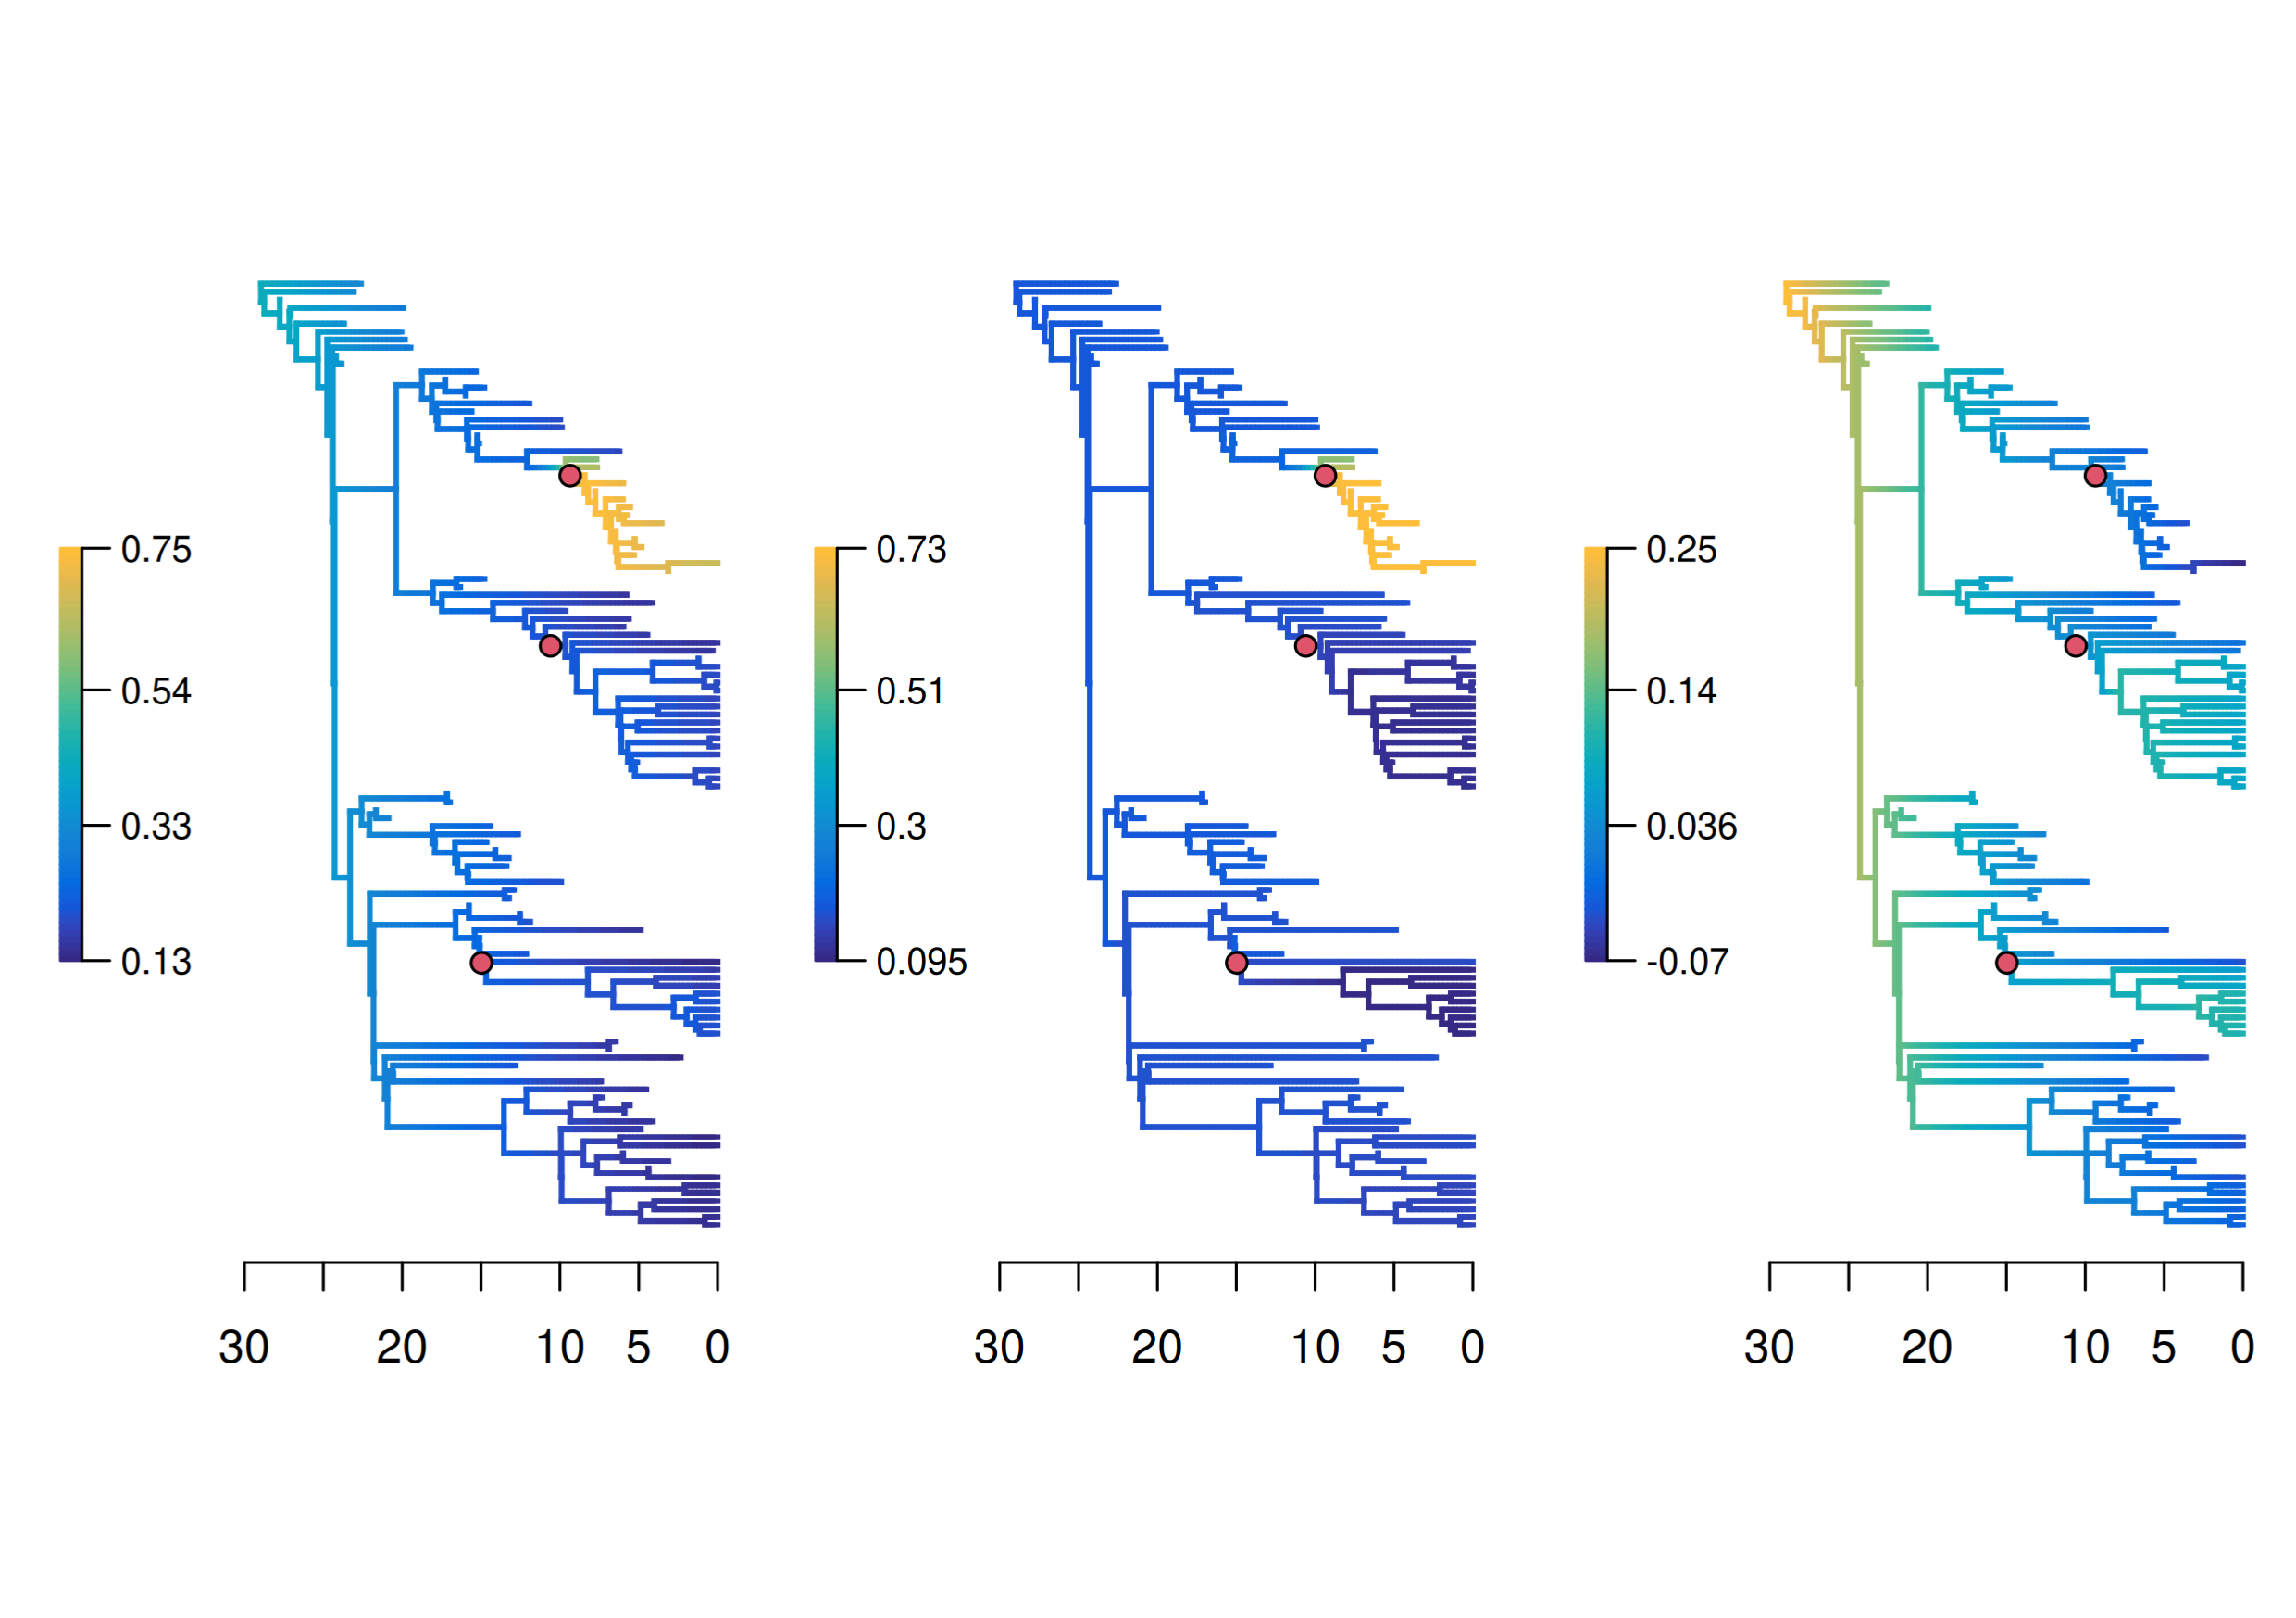
\includegraphics[width = \linewidth]{figures/diversification/main-analysis-with-sampled-ancestors/main-analysis-with-sampled-ancestors.png}
  \caption{Including sampled ancestors. $\lambda_{prior} = 1$. Left, middle and right panels indicate speciation, extinction and net diversification rates, respectively.}
  \label{fig-full-1}
\end{figure}

\subsubsection{$\lambda_{prior} = 2$}

% figure
\begin{figure}[H]
  \centering
  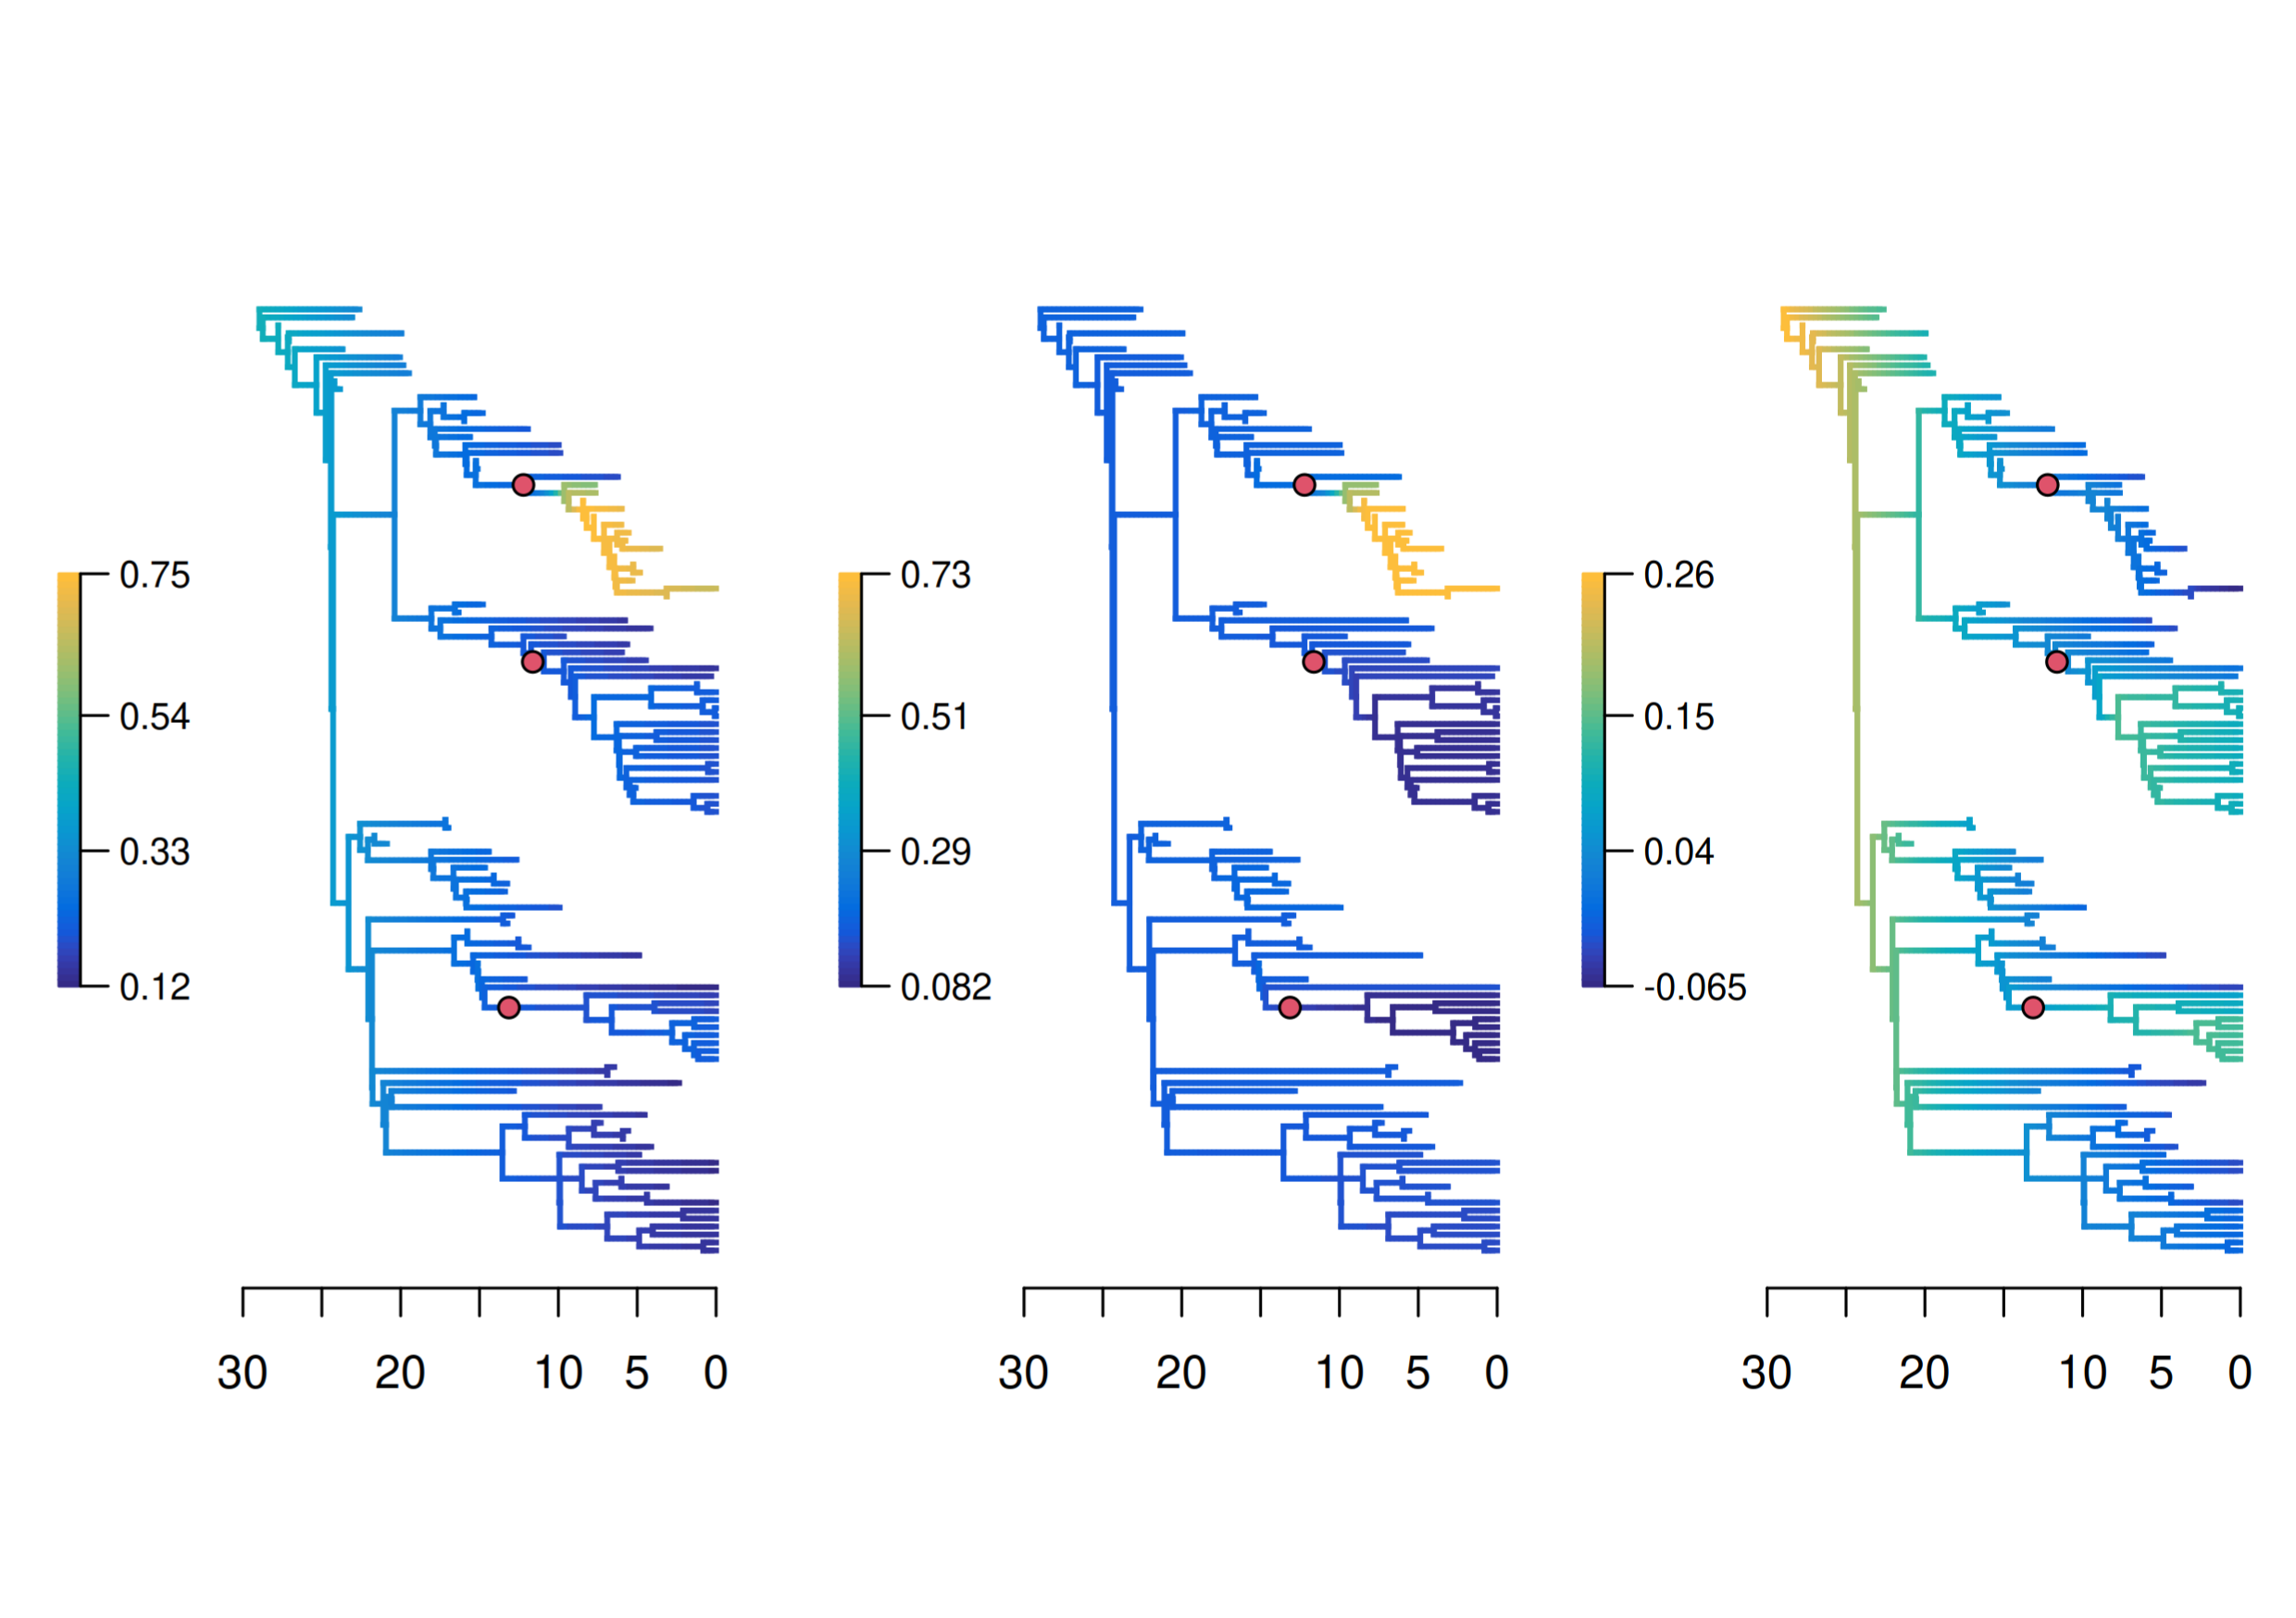
\includegraphics[width = \linewidth]{figures/diversification/sensitivity-analyses-with-sampled-ancestors/shifts-2/sensitivity-analysis-with-sampled-ancestors-2.png}
  \caption{Including sampled ancestors. $\lambda_{prior} = 2$. Left, middle and right panels indicate speciation, extinction and net diversification rates, respectively.}
  \label{fig-full-2}
\end{figure}

\subsubsection{$\lambda_{prior} = 10$}

% figure
\begin{figure}[H]
  \centering
  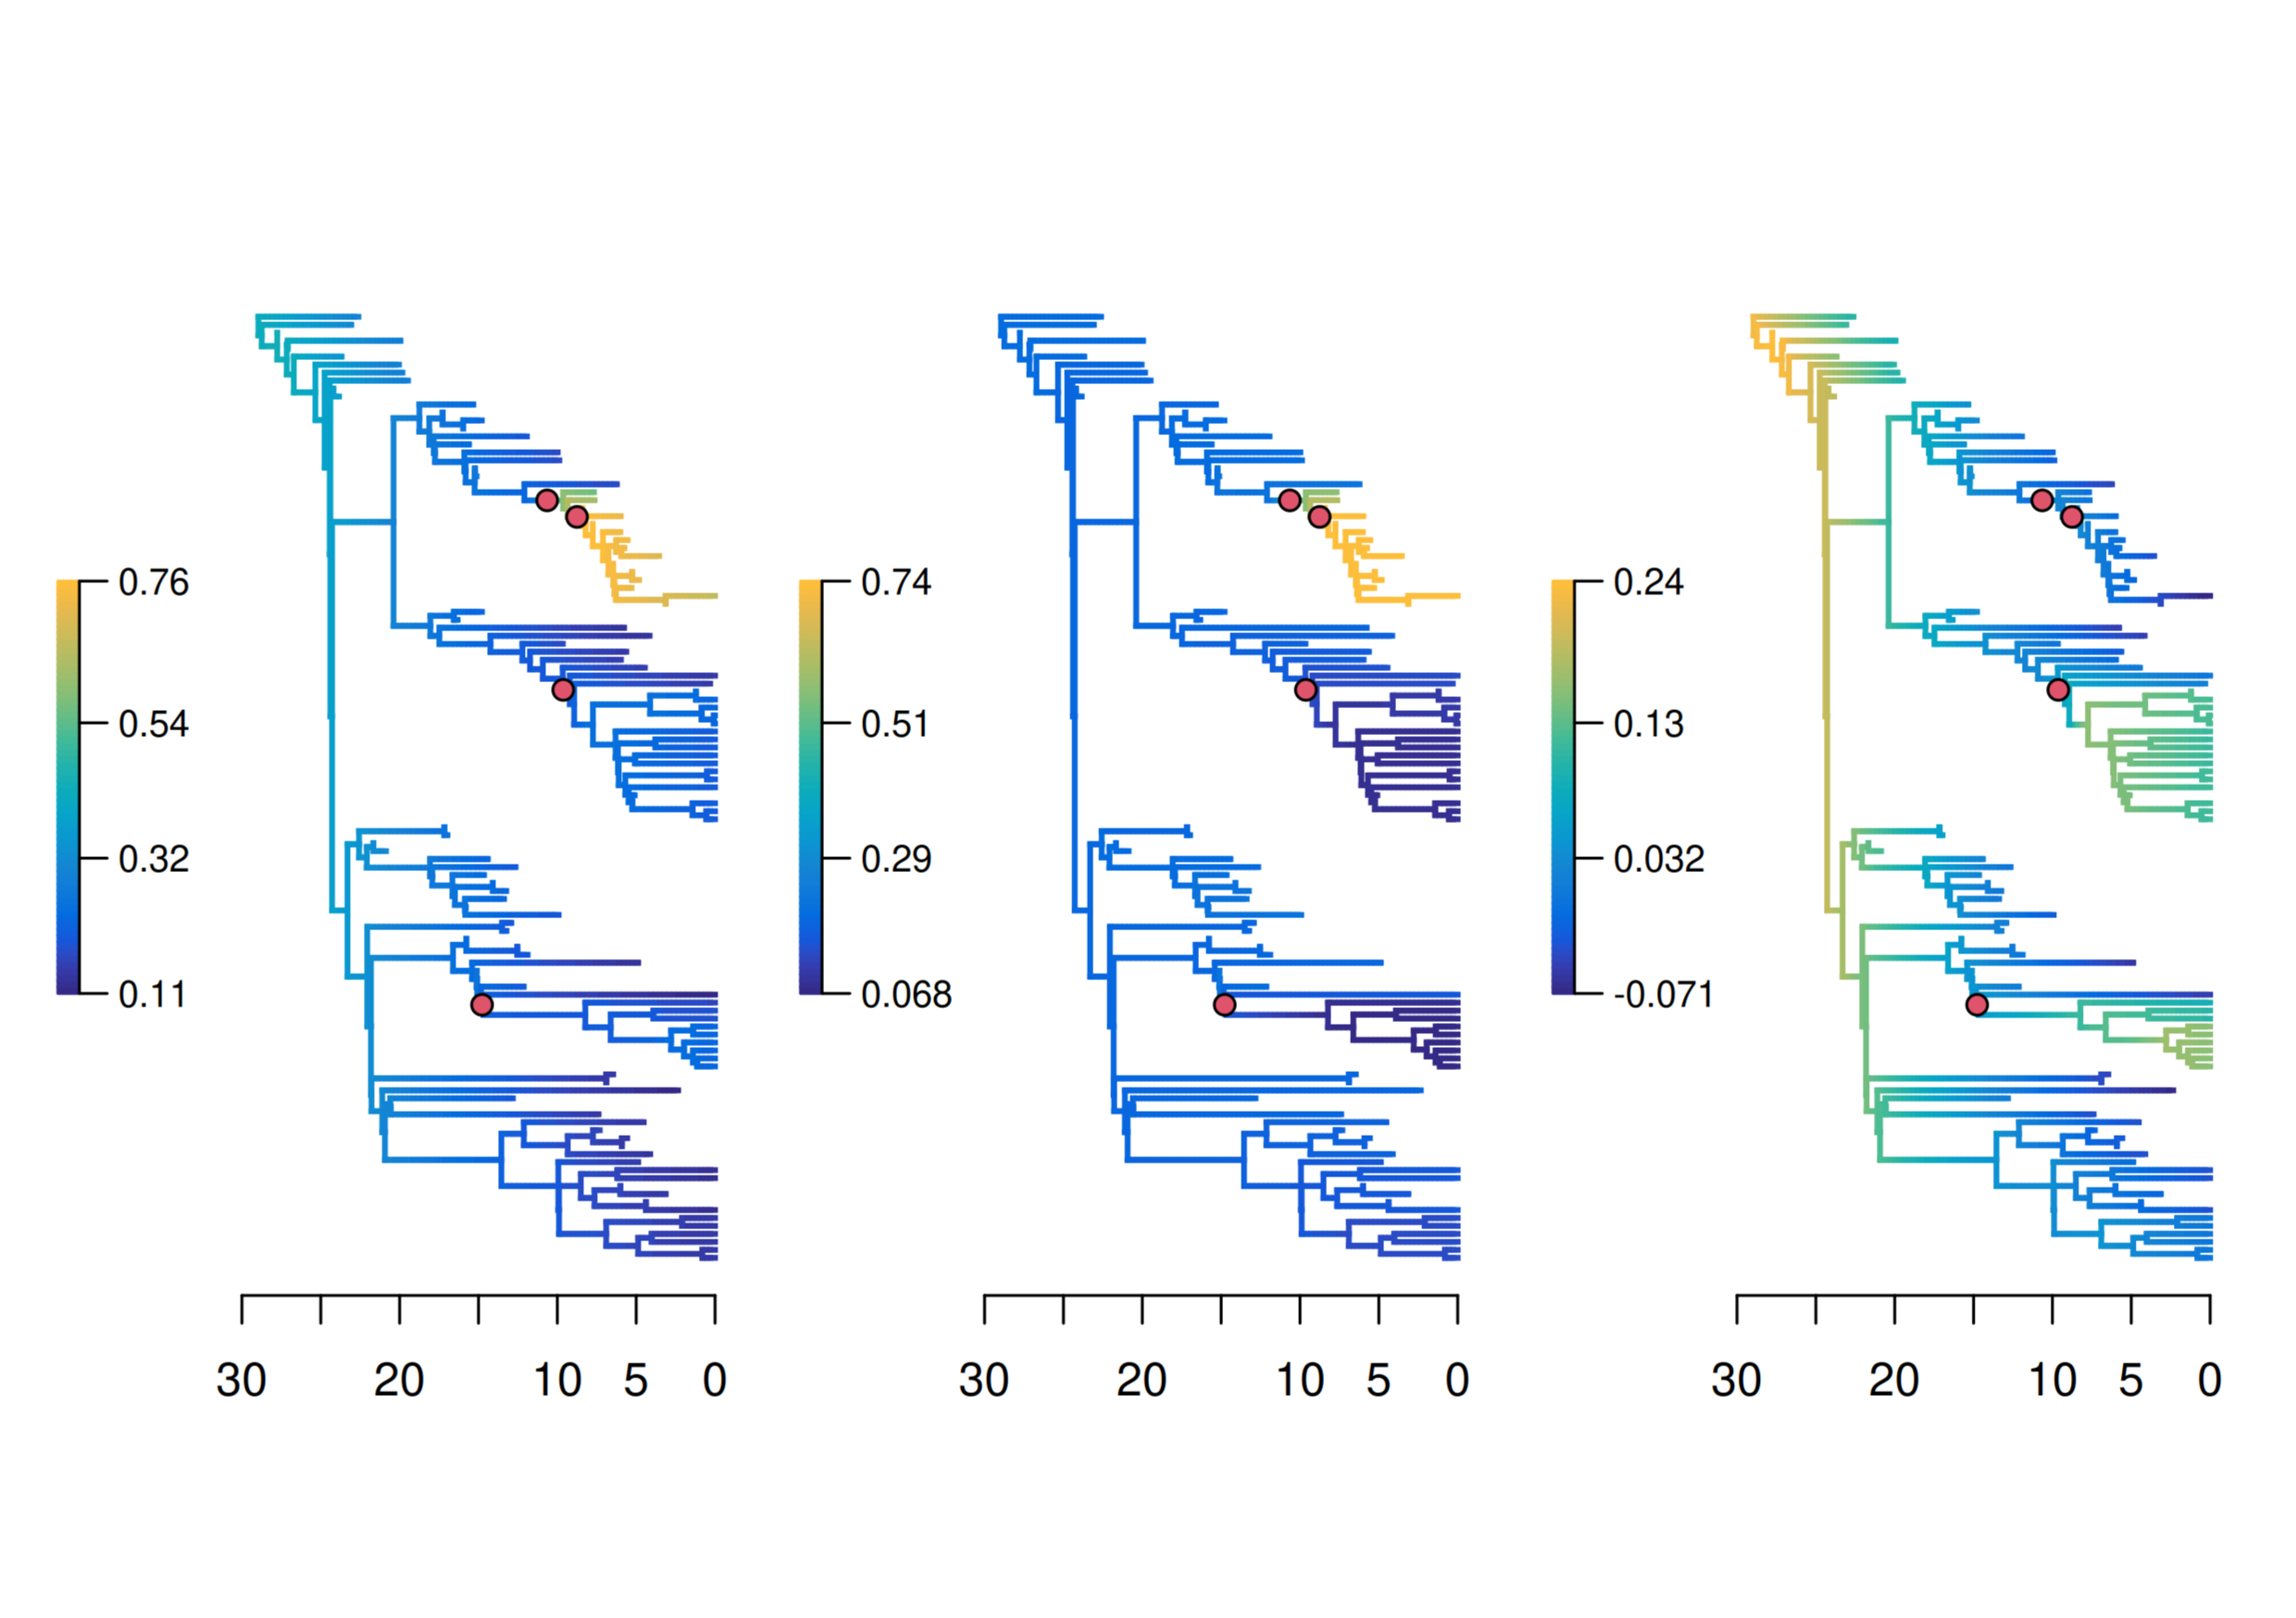
\includegraphics[width = \linewidth]{figures/diversification/sensitivity-analyses-with-sampled-ancestors/shifts-10/sensitivity-analysis-with-sampled-ancestors-10.png}
  \caption{Including sampled ancestors. $\lambda_{prior} = 10$. Left, middle and right panels indicate speciation, extinction and net diversification rates, respectively.}
  \label{fig-full-10}
\end{figure}


%-------------------------------------------------------------------------------
% Biogeography
%-----------------------------------------------------------------------------------
\newpage
\begin{landscape}
\section{Biogeographical history}
\subsection{Data and supplementary tables}

% Table of biogeography data
\begin{longtable}{llccccccccccp{0.6\textwidth}}

\caption{Biogeography data table for all 120 taxa included in the biogeographical history analyses. (A) Northern Pacific Ocean, (B) Eastern South Pacific Ocean, (C) Australasian seas and coastal waters, (D) Northern Atlantic Ocean, (E) Southern Atlantic Ocean, (F) Indian Ocean, (G) Southern Ocean, (H) Arctic Ocean, and (I) Paratethys/Mediterranean Ocean. Status defines the taxa as Extant or Fossil. Total gives the total number of areas each taxon is present within.}\\

\hline
\textbf{Taxon} & \textbf{Status} & \textbf{A} & \textbf{B} & \textbf{C} & \textbf{D} & \textbf{E} & \textbf{F}
& \textbf{G} & \textbf{H} & \textbf{I} & \textbf{Total} & \textbf{Notes}\\
\hline 
\textit{Arctocephalus australis} &
Extant  &
0 &
1 &
0 &
0 &
1 &
0 &
0 &
0 &
0 &
2  &
\\

\textit{Arctocephalus forsteri} &
Extant  &
0 &
0 &
1 &
0 &
0 &
1 &
0 &
0 &
0 &
2  &
\\

\textit{Arctocephalus galapagoensis} &
Extant &
0 &
1 &
0 &
0 &
0 &
0 &
0 &
0 &
0 &
1 &
\\

\textit{Arctocephalus gazella} &
Extant &
0 &
0 &
0 &
0 &
0 &
0 &
1 &
0 &
0 &
1 &
\\

\textit{Arctocephalus philippii} &
Extant &
0 &
1 &
0 &
0 &
0 &
0 &
0 &
0 &
0 &
1 &
\\

\textit{Arctocephalus pusillus} &
Extant &
0 &
0 &
1 &
0 &
1 &
1 &
0 &
0 &
0 &
3 &
\\

\textit{Arctocephalus townsendi} &
Extant &
1 &
0 &
0 &
0 &
0 &
0 &
0 &
0 &
0 &
1 &
\\

\textit{Arctocephalus tropicalis} &
Extant &
0 &
0 &
0 &
0 &
1 &
1 &
1 &
0 &
0 &
3 &
\\

\textit{Callorhinus ursinus} &
Extant &
1 &
0 &
0 &
0 &
0 &
0 &
0 &
0 &
0 &
1 &
\\

\textit{Cystophora cristata} &
Extant &
0 &
0 &
0 &
1 &
0 &
0 &
0 &
1 &
0 &
2 &
\\

\textit{Erignathus barbatus} &
Extant &
1 &
0 &
0 &
1 &
0 &
0 &
0 &
1 &
0 &
3 &
\\

\textit{Eumetopias jubatus} &
Extant &
1 &
0 &
0 &
0 &
0 &
0 &
0 &
0 &
0 &
1 &
\\

\textit{Halichoerus grypus} &
Extant &
0 &
0 &
0 &
1 &
0 &
0 &
0 &
1 &
0 &
2 &
\\

\textit{Histriophoca fasciata} &
Extant &
1 &
0 &
0 &
0 &
0 &
0 &
0 &
1 &
0 &
2 &
\\

\textit{Hydrurga leptonyx} &
Extant &
0 &
0 &
0 &
0 &
0 &
0 &
1 &
0 &
0 &
1 &
\\

\textit{Leptonychotes weddellii} &
Extant &
0 &
0 &
0 &
0 &
0 &
0 &
1 &
0 &
0 &
1 &
\\

\textit{Lobodon carcinophaga} &
Extant &
0 &
0 &
0 &
0 &
0 & 
0 &
1 &
0 &
0 &
1 &
\\

\textit{Mirounga angustirostris} &
Extant &
1 &
0 &
0 &
0 &
0 &
0 &
0 &
0 &
0 &
1 &
\\

\textit{Mirounga leonina} &
Extant &
0 &
1 &
1 &
0 &
0 &
0 &
1 &
0 &
0 &
3 &
\\

\textit{Monachus monachus} &
Extant &
0 &
0 &
0 &
1 &
0 &
0 &
0 &
0 &
1 &
2 &
\\

\textit{Neomonachus schauinslandi} &
Extant &
1 &
0 &
0 &
0 &
0 &
0 &
0 &
0 &
0 &
1 &
\\


\textit{Neomonachus tropicalis} &
Extant &
0 &
0 &
0 &
1 &
0 &
0 &
0 &
0 &
0 &
1 &
\\

\textit{Neophoca cinerea} &
Extant &
0 &
0 &
1 &
0 &
0 &
1 &
0 &
0 &
0 &
2 &
\\

\textit{Odobenus rosmarus} &
Extant &
1 &
0 &
0 &
0 &
0 &
0 &
0 &
1 &
0 &
2 &
Bering Sea counts as North Pacific\\

\textit{Ommatophoca rossii} &
Extant &
0 &
0 &
0 &
0 &
0 &
0 &
1 &
0 &
0 &
1 &
\\

\textit{Otaria byronia} &
Extant &
0 &
1 &
0 &
0 &
1 &
0 &
0 &
0 &
0 &
2 &
\\

\textit{Pagophilus groenlandica} &
Extant &
0 &
0 &
0 &
1 &
0 &
0 &
0 &
1 &
0 &
2 &
\\

\textit{Phoca largha} &
Extant &
1 &
0 &
0 &
0 &
0 &
0 &
0 &
1 &
0 &
2 &
Bering Sea counts as North Pacific\\

\textit{Phoca vitulina} &
Extant &
1 &
0 &
0 &
1 &
0 &
0 &
0 &
1 &
0 &
3 &
\\

\textit{Phocarctos hookeri} &
Extant &
0 &
0 &
1 &
0 &
0 &
0 &
0 &
0 &
0 &
1 &
\\

\textit{Pusa caspica} &
Extant &
0 &
0 &
0 &
0 &
0 &
0 &
0 &
0 &
1 &
1 &
Caspian sea was part of Parathethys\\

\textit{Pusa hispida} &
Extant &
1 &
0 &
0 &
1 &
0 &
0 &
0 &
1 &
0 &
3 &
\\

\textit{Zalophus californianus} &
Extant &
1 &
0 &
0 &
0 &
0 &
0 &
0 &
0 &
0 &
1 &
\\

\textit{Zalophus japonicus} &
Extant &
1 &
0 &
0 &
0 &
0 &
0 &
0 &
0 &
0 &
1 &
\\

\textit{Zalophus wollebaeki} &
Extant &
0 &
1 &
0 &
0 &
0 &
0 &
0 &
0 &
0 &
1 &
\\

\textit{Acrophoca longirostris} &
Fossil &
0 &
1 &
0 &
0 &
0 &
0 &
0 &
0 &
0 &
1 &
\\

\textit{Aivukus cedrosensis} &
Fossil &
1 &
0 &
0 &
0 &
0 &
0 &
0 &
0 &
0 &
1 &
\\

\textit{Allodesmus demerei} &
Fossil &
1 &
0 &
0 &
0 &
0 &
0 &
0 &
0 &
0 &
1 &
\\

\textit{Allodesmus kernensis} &
Fossil &
1 &
0 &
0 &
0 &
0 &
0 &
0 &
0 &
0 &
1 &
\\

\textit{Allodesmus naorai} &
Fossil &
1 &
0 &
0 &
0 &
0 &
0 &
0 &
0 &
0 &
1 &
\\

\textit{Allodesmus packardi} &
Fossil &
1 &
0 &
0 & 
0 &
0 &
0 &
0 &
0 &
0 &
1 &
\\

\textit{Allodesmus sinanoensis} &
Fossil &
1 &
0 &
0 &
0 &
0 &
0 &
0 &
0 &
0 &
1 &
\\

\textit{Allodesmus uraiporensis} &
Fossil &
1 &
0 &
0 &
0 &
0 &
0 &
0 &
0 &
0 &
1 &
\\

\textit{Allodesmus sp cf sadoensis} &
Fossil &
1 &
0 &
0 &
0 &
0 &
0 &
0 &
0 &
0 &
1 &
\\

\textit{Archaeodobenus akamatsui} &
Fossil &
1 &
0 &
0 &
0 &
0 &
0 &
0 &
0 &
0 &
1 &
\\

\textit{Atopotarus courseni} &
Fossil &
1 &
0 &
0 &
0 &
0 &
0 &
0 &
0 &
0 &
1 &
\\

\textit{Australophoca changorum} &
Fossil &
0 &
1 &
0 &
0 &
0 &
0 &
0 &
0 &
0 &
1 &
\\

\textit{Callorhinus gilmorei} &
Fossil &
1 &
0 &
0 &
0 &
0 &
0 &
0 &
0 &
0 &
1 &
\\

\textit{Desmatophoca brachycephala} &
Fossil &
1 &
0 &
0 &
0 &
0 &
0 &
0 &
0 &
0 &
1 &
\\

\textit{Desmatophoca oregonensis} &
Fossil &
1 &
0 &
0 &
0 &
0 &
0 &
0 &
0 &
0 &
1 &
\\

Desmatophocidae indet &
Fossil &
1 &
0 &
0 &
0 &
0 &
0 &
0 &
0 &
0 &
1 &
Desmatophocidae indet USNM 335445\\

\textit{Devinophoca claytoni} &
Fossil &
0 &
0 &
0 &
0 &
0 &
0 &
0 &
0 &
1 &
1 &
\\

\textit{Devinophoca emryi} &
Fossil &
0 &
0 &
0 &
0 &
0 &
0 &
0 &
0 &
1 &
1 &
\\

\textit{Dusignathus santacruzensis} &
Fossil &
1 &
0 &
0 &
0 &
0 &
0 &
0 &
0 &
0 &
1 &
\\

\textit{Dusignathus seftoni} &
Fossil &
1 &
0 &
0 &
0 &
0 &
0 &
0 &
0 &
0 &
1 &
\\

\textit{Enaliarctos barnesi} &
Fossil &
1 &
0 &
0 &
0 &
0 &
0 &
0 &
0 &
0 &
1 &
\\

\textit{Enaliarctos emlongi} &
Fossil &
1 &
0 &
0 &
0 &
0 &
0 &
0 &
0 &
0 &
1 &
\\

\textit{Enaliarctos mealsi} &
Fossil &
1 &
0 &
0 &
0 &
0 &
0 &
0 &
0 &
0 &
1 &
\\

\textit{Enaliarctos mitchelli} &
Fossil &
1 &
0 &
0 &
0 &
0 &
0 &
0 &
0 &
0 &
1 &
\\

\textit{Enaliarctos tedfordi} &
Fossil &
1 &
0 &
0 &
0 &
0 &
0 &
0 &
0 &
0 &
1 &
\\

\textit{Eodesmus condoni} &
Fossil &
1 &
0 &
0 &
0 &
0 &
0 &
0 &
0 &
0 &
1 &
\\

\textit{Eomonachus belegaerensis} &
Fossil &
0 &
0 &
1 &
0 &
0 &
0 &
0 &
0 &
0 &
1 &
\\

\textit{Eotaria citrica} &
Fossil &
1 &
0 &
0 &
0 &
0 &
0 &
0 &
0 &
0 &
1 &
\\

\textit{Eotaria crypta} &
Fossil &
1 &
0 &
0 &
0 &
0 &
0 &
0 &
0 &
0 &
1 &
\\

\textit{Frisiphoca aberratum} &
Fossil &
0 &
0 &
0 &
1 &
0 &
0 &
0 &
0 &
0 &
1 &
\\

\textit{Frisiphoca affine} &
Fossil &
0 &
0 &
0 &
1 &
0 &
0 &
0 &
0 &
0 &
1 &
\\

\textit{Gomphotaria pugnax} &
Fossil &
1 &
0 &
0 &
0 &
0 &
0 &
0 &
0 &
0 &
1 &
\\

\textit{Hadrokirus martini} &
Fossil &
0 &
1 &
0 &
0 &
0 &
0 &
0 &
0 &
0 &
1 &
\\

\textit{Homiphoca capensis} &
Fossil &
0 &
0 &
0 &
0 &
1 &
0 &
0 &
0 &
0 &
1 &
Not coded as North Atlantic as Spanish material is dubious\\

aff \textit{Homiphoca capensis} &
Fossil &
0 &
0 &
0 &
1 &
0 &
0 &
0 &
0 &
0 &
1 &
Phocidae aff \textit{Homiphoca capensis} USNM\\

\textit{Homiphoca sp} &
Fossil &
0 &
0 &
0 &
0 &
1 &
0 &
0 &
0 &
0 &
1 &
Combined \textit{Homiphoca sp} SAM PQL 30080, 32415, 31976, 32101, 30568 as one taxon\\

\textit{Hydrarctos lomasiensis} &
Fossil &
0 &
1 &
0 &
0 &
0 &
0 &
0 &
0 &
0 &
1 &
\\

\textit{Imagotaria downsi} &
Fossil &
1 &
0 &
0 &
0 &
0 &
0 &
0 &
0 &
0 &
1 &
\\

\textit{Kamtschatarctos sinelnikovae} &
Fossil &
1 &
0 &
0 &
0 &
0 &
0 &
0 &
0 &
0 &
1 &
\\

\textit{Kawas benegasorum} &
Fossil &
0 &
0 &
0 &
0 &
1 &
0 &
0 &
0 &
0 &
1 &
\\

\textit{Leptophoca proxima} &
Fossil &
0 &
0 &
0 &
1 &
0 &
0 &
0 &
0 &
1 &
2 &
\\

cf Miroungini indet &
Fossil &
0 &
0 &
1 &
0 &
0 &
0 &
0 &
0 &
0 &
1 &
cf Miroungini indet CD 35\\

Monachini indet &
Fossil &
0 &
0 &
1 &
0 &
0 &
0 &
0 &
0 &
0 &
1 &
Monachini indet NMV P160399\\

\textit{Nanophoca vitulinoides} &
Fossil &
0 &
0 &
0 &
1 &
0 &
0 &
0 &
0 &
0 &
1 &
\\

\textit{Neophoca palatina} &
Fossil &
0 &
0 &
1 &
0 &
0 &
0 &
0 &
0 &
0 &
1 &
\\

\textit{Neotherium mirum} &
Fossil &
1 &
0 &
0 &
0 &
0 &
0 &
0 &
0 &
0 &
1 &
\\

\textit{Noriphoca gaudini} &
Fossil &
0 &
0 &
0 &
0 &
0 &
0 &
0 & 
0 &
1 &
1 &
\\

Odobenidae indet &
Fossil &
1 &
0 &
0 &
0 &
0 &
0 &
0 &
0 &
0 &
1 &
Odobenidae gen et spec indet LACM 135920\\

\textit{Ontocetus emmonsi} &
Fossil &
0 &
0 &
0 &
1 &
0 &
0 &
0 &
0 &
0 &
1 &
\\

\textit{Osodobenus eodon} &
Fossil &
1 &
0 &
0 &
0 &
0 &
0 &
0 &
0 &
0 &
1 &
\\

\textit{Pelagiarctos thomasi} &
Fossil &
1 &
0 &
0 &
0 &
0 &
0 &
0 &
0 &
0 &
1 &
\\

\textit{Pelagiarctos sp} &
Fossil &
1 &
0 &
0 &
0 &
0 &
0 &
0 &
0 &
0 &
1 &
\textit{Pelagiarctos sp} SDNHM 131041\\

\textit{Pinnarctidion bishopi} &
Fossil &
1 &
0 &
0 &
0 &
0 &
0 &
0 &
0 &
0 &
1 &
\\

\textit{Pinnarctidion iverseni} &
Fossil &
1 &
0 &
0 &
0 &
0 &
0 &
0 &
0 &
0 &
1 &
\\

\textit{Pinnarctidion rayi} &
Fossil &
1 &
0 &
0 &
0 &
0 &
0 &
0 &
0 &
0 &
1 &
\\

\textit{Pithanotaria starri} &
Fossil &
1 &
0 &
0 &
0 &
0 &
0 &
0 &
0 &
0 &
1 &
\\

\textit{Pliopedia pacifica} &
Fossil &
1 &
0 &
0 &
0 &
0 &
0 &
0 &
0 &
0 &
1 &
\\

\textit{Pliophoca etrusca} &
Fossil &
0 &
0 &
0 &
0 &
0 &
0 &
0 &
0 &
1 &
1 &
\\

\textit{Pliophoca etrusca USNM} &
Fossil &
0 &
0 &
0 &
1 &
0 &
0 &
0 &
0 &
0 &
1 &
\textit{Pliophoca etrusca} USNM 171221 et 181419 et 181504 et 187580 et 243697 et 250290 et 254327 et 34734\\

\textit{Pontolis barroni} &
Fossil &
1 &
0 &
0 &
0 &
0 &
0 &
0 &
0 &
0 &
1 &
\\

\textit{Pontolis} cf &
Fossil &
1 &
0 &
0 &
0 &
0 &
0 &
0 &
0 &
0 &
1 &
\\

\textit{Pontolis kohnoi} &
Fossil &
1 &
0 &
0 &
0 &
0 &
0 &
0 &
0 &
0 &
1 &
\\

\textit{Pontolis magnus} &
Fossil &
1 &
0 &
0 &
0 &
0 &
0 &
0 &
0 &
0 &
1 &
\\

\textit{Potamotherium vallentoni} &
Fossil &
0 &
0 &
0 &
1 &
0 &
0 &
0 &
0 &
0 &
1 &
\\

\textit{Praepusa boeska} &
Fossil &
0 &
0 &
0 &
0 &
0 &
0 &
0 &
0 &
1 &
1 &
\\

\textit{Praepusa magyaricus} &
Fossil &
0 &
0 &
0 &
0 &
0 &
0 &
0 &
0 &
1 &
1 &
\\

\textit{Praepusa pannonica} &
Fossil &
0 &
0 &
0 &
1 &
0 &
0 &
0 &
0 &
1 &
2 &
\\

\textit{Praepusa vindobonensis} &
Fossil &
0 &
0 &
0 &
0 &
0 &
0 &
0 &
0 &
1 &
1 &
\\

\textit{Proneotherium repenningi} &
Fossil &
1 &
0 &
0 &
0 &
0 &
0 &
0 &
0 &
0 &
1 &
\\

\textit{Properiptychus argentinus} &
Fossil &
0 &
0 &
0 &
0 &
1 &
0 &
0 &
0 &
0 &
1 &
\\

\textit{Proterozetes ulysses} &
Fossil &
1 &
0 &
0 &
0 &
0 &
0 &
0 &
0 &
0 &
1 &
\\

\textit{Protodobenus japonicus} &
Fossil &
1 &
0 &
0 &
0 &
0 &
0 &
0 &
0 &
0 &
1 &
\\

\textit{Prototaria planicephala} &
Fossil &
1 &
0 &
0 &
0 &
0 &
0 &
0 &
0 &
0 &
1 &
\\

\textit{Prototaria primigena} &
Fossil &
1 &
0 &
0 &
0 &
0 &
0 &
0 &
0 &
0 &
1 &
\\

\textit{Pseudotaria muramotoi} &
Fossil &
1 &
0 &
0 &
0 &
0 &
0 &
0 &
0 &
0 &
1 &
\\

\textit{Piscophoca pacifica} &
Fossil &
0 &
1 &
0 &
0 &
0 &
0 &
0 &
0 &
0 &
1 &
\\

\textit{Pteronarctos goedertae} &
Fossil &
1 &
0 &
0 &
0 &
0 &
0 &
0 &
0 &
0 &
1 &
\\

\textit{Puijila darwini} &
Fossil &
0 &
0 &
0 &
0 &
0 &
0 &
0 &
1 &
0 &
1 &
\\

\textit{Sarcodectes magnus} &
Fossil &
0 &
0 &
0 &
1 &
0 &
0 &
0 &
0 &
0 &
1 &
\\

cf \textit{Thalassoleon}&
Fossil &
1 &
0 &
0 &
0 &
0 &
0 &
0 &
0 &
0 &
1 &
\\

\textit{Thalassoleon inouei} &
Fossil &
1 &
0 &
0 &
0 &
0 &
0 &
0 &
0 &
0 &
1 &
\\

\textit{Thalassoleon macnallyae} &
Fossil &
1 &
0 &
0 &
0 &
0 &
0 &
0 &
0 &
0 &
1 &
\\

\textit{Thalassoleon mexicanus} &
Fossil &
1 &
0 &
0 &
0 &
0 &
0 &
0 &
0 &
0 &
1 &
\\

\textit{Titanotaria orangensis} &
Fossil &
1 &
0 &
0 &
0 &
0 &
0 &
0 &
0 &
0 &
1 &
\\

\textit{Valenictus chulavistensis} &
Fossil &
1 &
0 &
0 &
0 &
0 &
0 &
0 &
0 &
0 &
1 &
\\
\hline

\label{table-biogeo-data}
\end{longtable}

\newpage
% Table of ocean pathways
\begin{longtable}{cp{0.4\textwidth}cp{0.7\textwidth}}

\caption{Key biogeographical dates in ocean pathways related to pinniped dispersal.}\\

\hline
\textbf{Time (Ma)} & \textbf{Event} & \textbf{Reference} & \textbf{Notes}\\
\hline
37.8 &
Bering Strait closure &
\cite{gladenkov2002refined} &
Loss of connection between Northern Pacific Ocean and Arctic Ocean \\
20.44 &
Closure of seaway between Paratethys and Indian Ocean &
\cite{rogl1999mediterranean} &
Loss of connection between Paratethys and Indian Ocean. No connection between Northern Pacific Ocean and Arctic Ocean \\  
15.97 &
Opening of seaway between Paratethys and Indian Ocean &
\cite{rogl1999mediterranean} &
Connection between Paratethys and Indian Ocean re-established. No connection between Northern Pacific Ocean and Arctic Ocean\\
13.82 &
Closure of seaway between Paratethys and Indian Ocean &
\cite{rogl1999mediterranean} &
Loss of connection between Paratethys and Indian Ocean. No connection between Northern Pacific Ocean and Arctic Ocean \\
11 &
Restriction of trans-oceanic circulation within the Central American Seaway &
\cite{duque1990neogene} &
No connection between Northern Pacific Ocean and Arctic Ocean, or Paratethys and Indian Ocean \\
6.3 &
Re-establishment of trans-oceanic circulation, Central American Seaway open &
\cite{duque1990neogene} &
No connection between Northern Pacific Ocean and Arctic Ocean, or Paratethys and Indian Ocean \\
5.97 &
Beginning of Messinian Salinity Crisis &
\cite{manzi2018onset, micallef2018evidence} &
Disappearance of Paratethys. No connection between Northern Pacific Ocean and Arctic Ocean \\
5.5 &
Caspian Sea basin forms &
\cite{kazmin2011} &
No Paratethys/Mediterranean. No connection between Northern Pacific Ocean and Arctic Ocean \\
5.33 &
End of Messinian Salinity Crisis &
\cite{manzi2018onset, micallef2018evidence} &
Paratethys/Mediterranean reappears along with the Caspian Sea. No connection between Northern Pacific Ocean and Arctic Ocean, or Paratethys/Mediterranean and Indian Ocean \\
5.32 &
Bering Strait reopens &
\cite{gladenkov2002refined} &
Connection between Northern Pacific Ocean and Arctic Ocean re-established. No connection between Paratethys/Mediterranean and the Indian Ocean\\
3.7 &
Closure of Central American Seaway, land bridge established &
\cite{duque1990neogene} &
Loss of connection between North Pacific Ocean and North Atlantic Ocean. No connection between  Paratethys/Mediterranean and the Indian Ocean \\
0.781 &
Pleistocene glacial maximum &
\cite{ehlers2007extent} &
Glaciation connects the Arctic Ocean to Lake Baikal. No connection between North Pacific Ocean and North Atlantic Ocean. No connection between Paratethys/Mediterranean and the Indian Ocean. \\
0 &
Modern oceanic pathways &
- &
No connection between North Pacific Ocean and North Atlantic Ocean. No connection between  Paratethys/Mediterranean and the Indian Ocean.\\
\hline

\label{table-pathways}
\end{longtable}

\newpage
% Table of impossible states
\begin{longtable}{lll}

\caption{Area-combinations that were excluded from the analyses for each time bin. (A) Northern Pacific Ocean, (B) Eastern South Pacific Ocean, (C) Australasian seas and coastal waters, (D) Northern Atlantic Ocean, (E) Southern Atlantic Ocean, (F) Indian Ocean, (G) Southern Ocean, (H) Arctic Ocean, and (I) Paratethys/Mediterranean Ocean. Note that state BE could not be coded as unlikely in the 0 - 3.7 Ma time bin as this prevented the model from fitting due to missing intermediate states.}\\

\hline
\textbf{Time bin (Ma)} & \textbf{Impossible} & \textbf{Unlikely}\\
\hline
20.44 - 37.8 &
AH &
AH \\
15.97 - 20.44  &
AH, FI &
AH, FI\\
13.82 - 15.97 & 
AH &
AH\\
5.97 - 13.82 &
AH, FI &
AH, FI\\
5.33 - 5.97  &
AH, AI, BI, CI, DI, EI, FI, GI, HI, I &
AE, AF, AG, BD, BE, BF, BH, CD, CE, CH, DF, DG, FH, GH\\
5.32 - 5.33 &
AH, FI &
AE, AF, AG, AI, BD, BE, BF, BH, BI, CD, CE, CH, CI, DF, DG, EI, FH, GH, GI\\ 
3.7 - 5.32 &
FI &
AE, AF, AG, AI, BD, BE, BF, BH, BI, CD, CE, CH, CI, DF, DG, EI, FH, GH, GI\\ 
0 - 3.7  &
AD, FI &
AE, AF, AG, AI, BD, BF, BH, BI, CD, CE, CH, CI, DF, DG, EI, FH, GH, GI\\
\hline

\label{table-states}
\end{longtable}

\end{landscape}
%----------------------------------------------
\subsection{Supplementary results}

% figure
\begin{figure}[H]
 \centering
  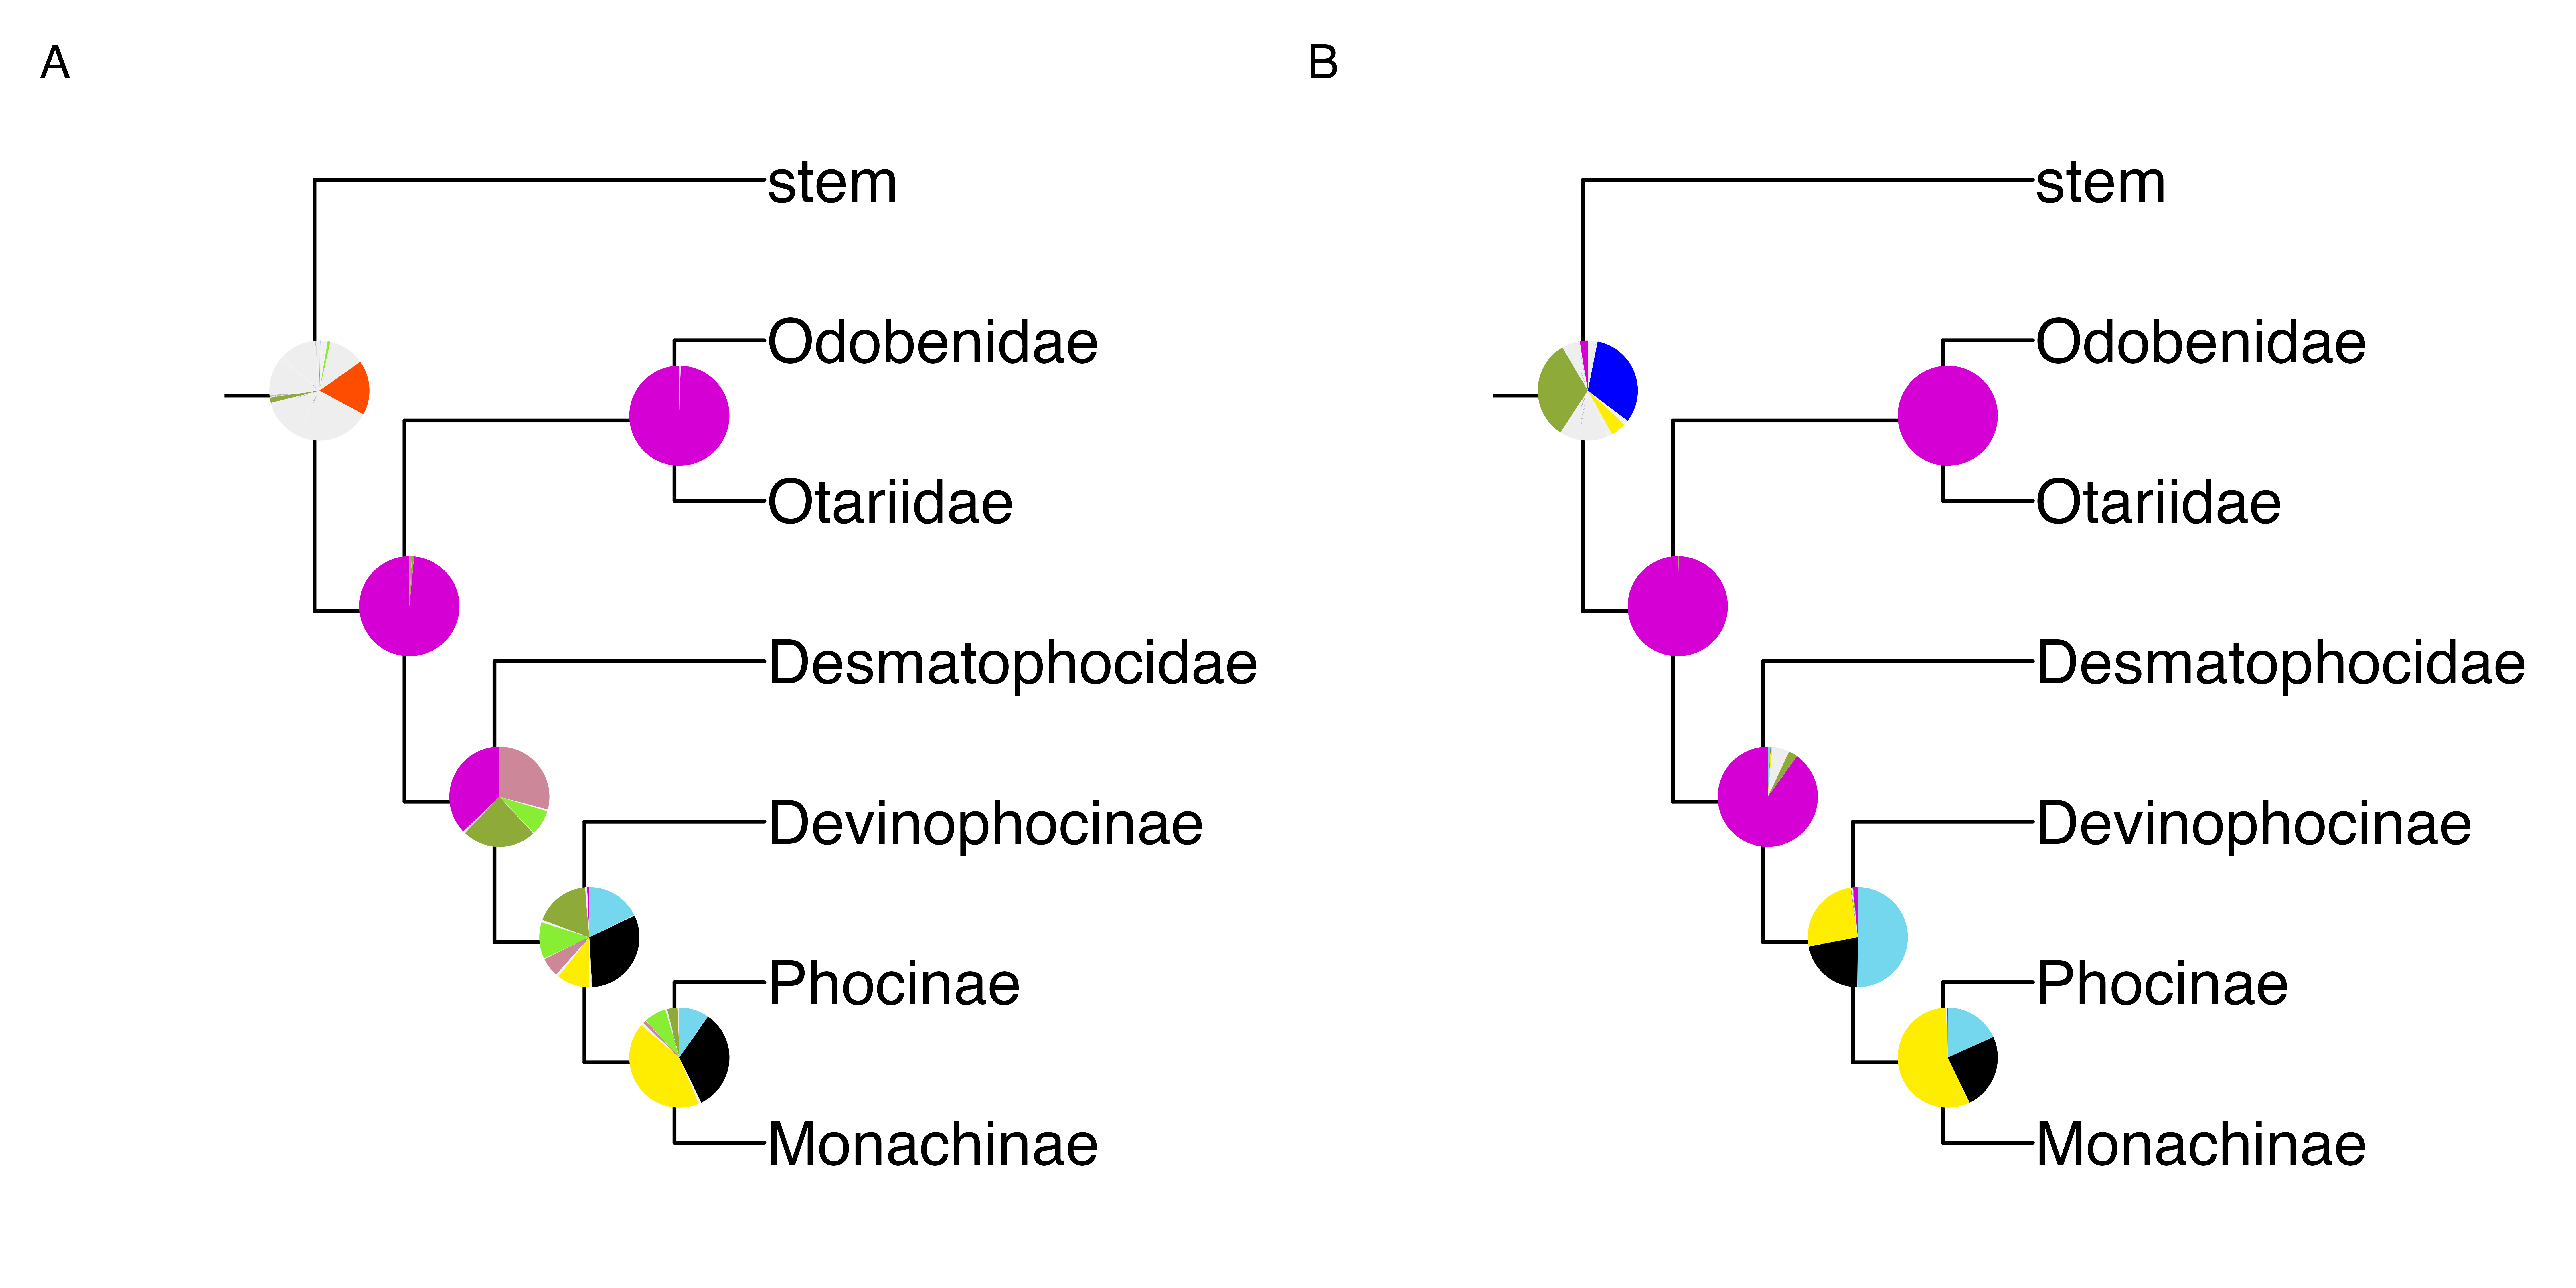
\includegraphics[width = \linewidth]{figures/biogeography-insets-two.png}
  \caption{Biogeographic state estimations for the major groups within our study. Pies show the relative proportions of different states at that node. See Figure \ref{fig-legend} for legend. States with proportions less than 0.1 are shown in gray. A) DEC; B) DEC+J (also in main text results).}
  \label{fig-nodes}
\end{figure} 

% table of unlikely results
% Table of unlikely results
\begin{longtable}{cccccc}

\caption{Results of model fits from BioGeoBEARS analysis for pinnipeds. Impossible and unlikely area-combinations were excluded (see text). DEC = dispersal-extinction-cladogenesis; DEC + J = DEC model with jump dispersal; lnL = log-likelihood values; AICc = sample-size corrected Akaike information criterion; d = dispersal rate (range expansion) along each branch within the phylogeny; e = extinction rate (range contraction) along each branch within the phylogeny; j, relative weight of jump dispersal in each model.
}\\

\hline
\textbf{Taxa} & 
\textbf{lnL} &
\textbf{AICc} &
\textbf{d}&
\textbf{e} &
\textbf{j}\\
\hline
DEC &
-275.4 &
554.7 &
0.0186 &
0.0230 &
-\\

DEC+J &
-244.8 &
495.6 &
0.0119 &
0.0026 &
0.0167\\

\hline

\label{table-unlikely}
\end{longtable}

A full set of the marginal probabilities of each state at each node can be found in the files *DEC-all-node-probabilities.csv* and 
*DECJ-all-node-probabilities.csv*. These are too large for this document so are included with the data at [removed to anonymise]. A tree with node labels for interpreting these results is available in Figure \ref{fig-node-labels}.

% figure
\begin{figure}[H]
 \centering
  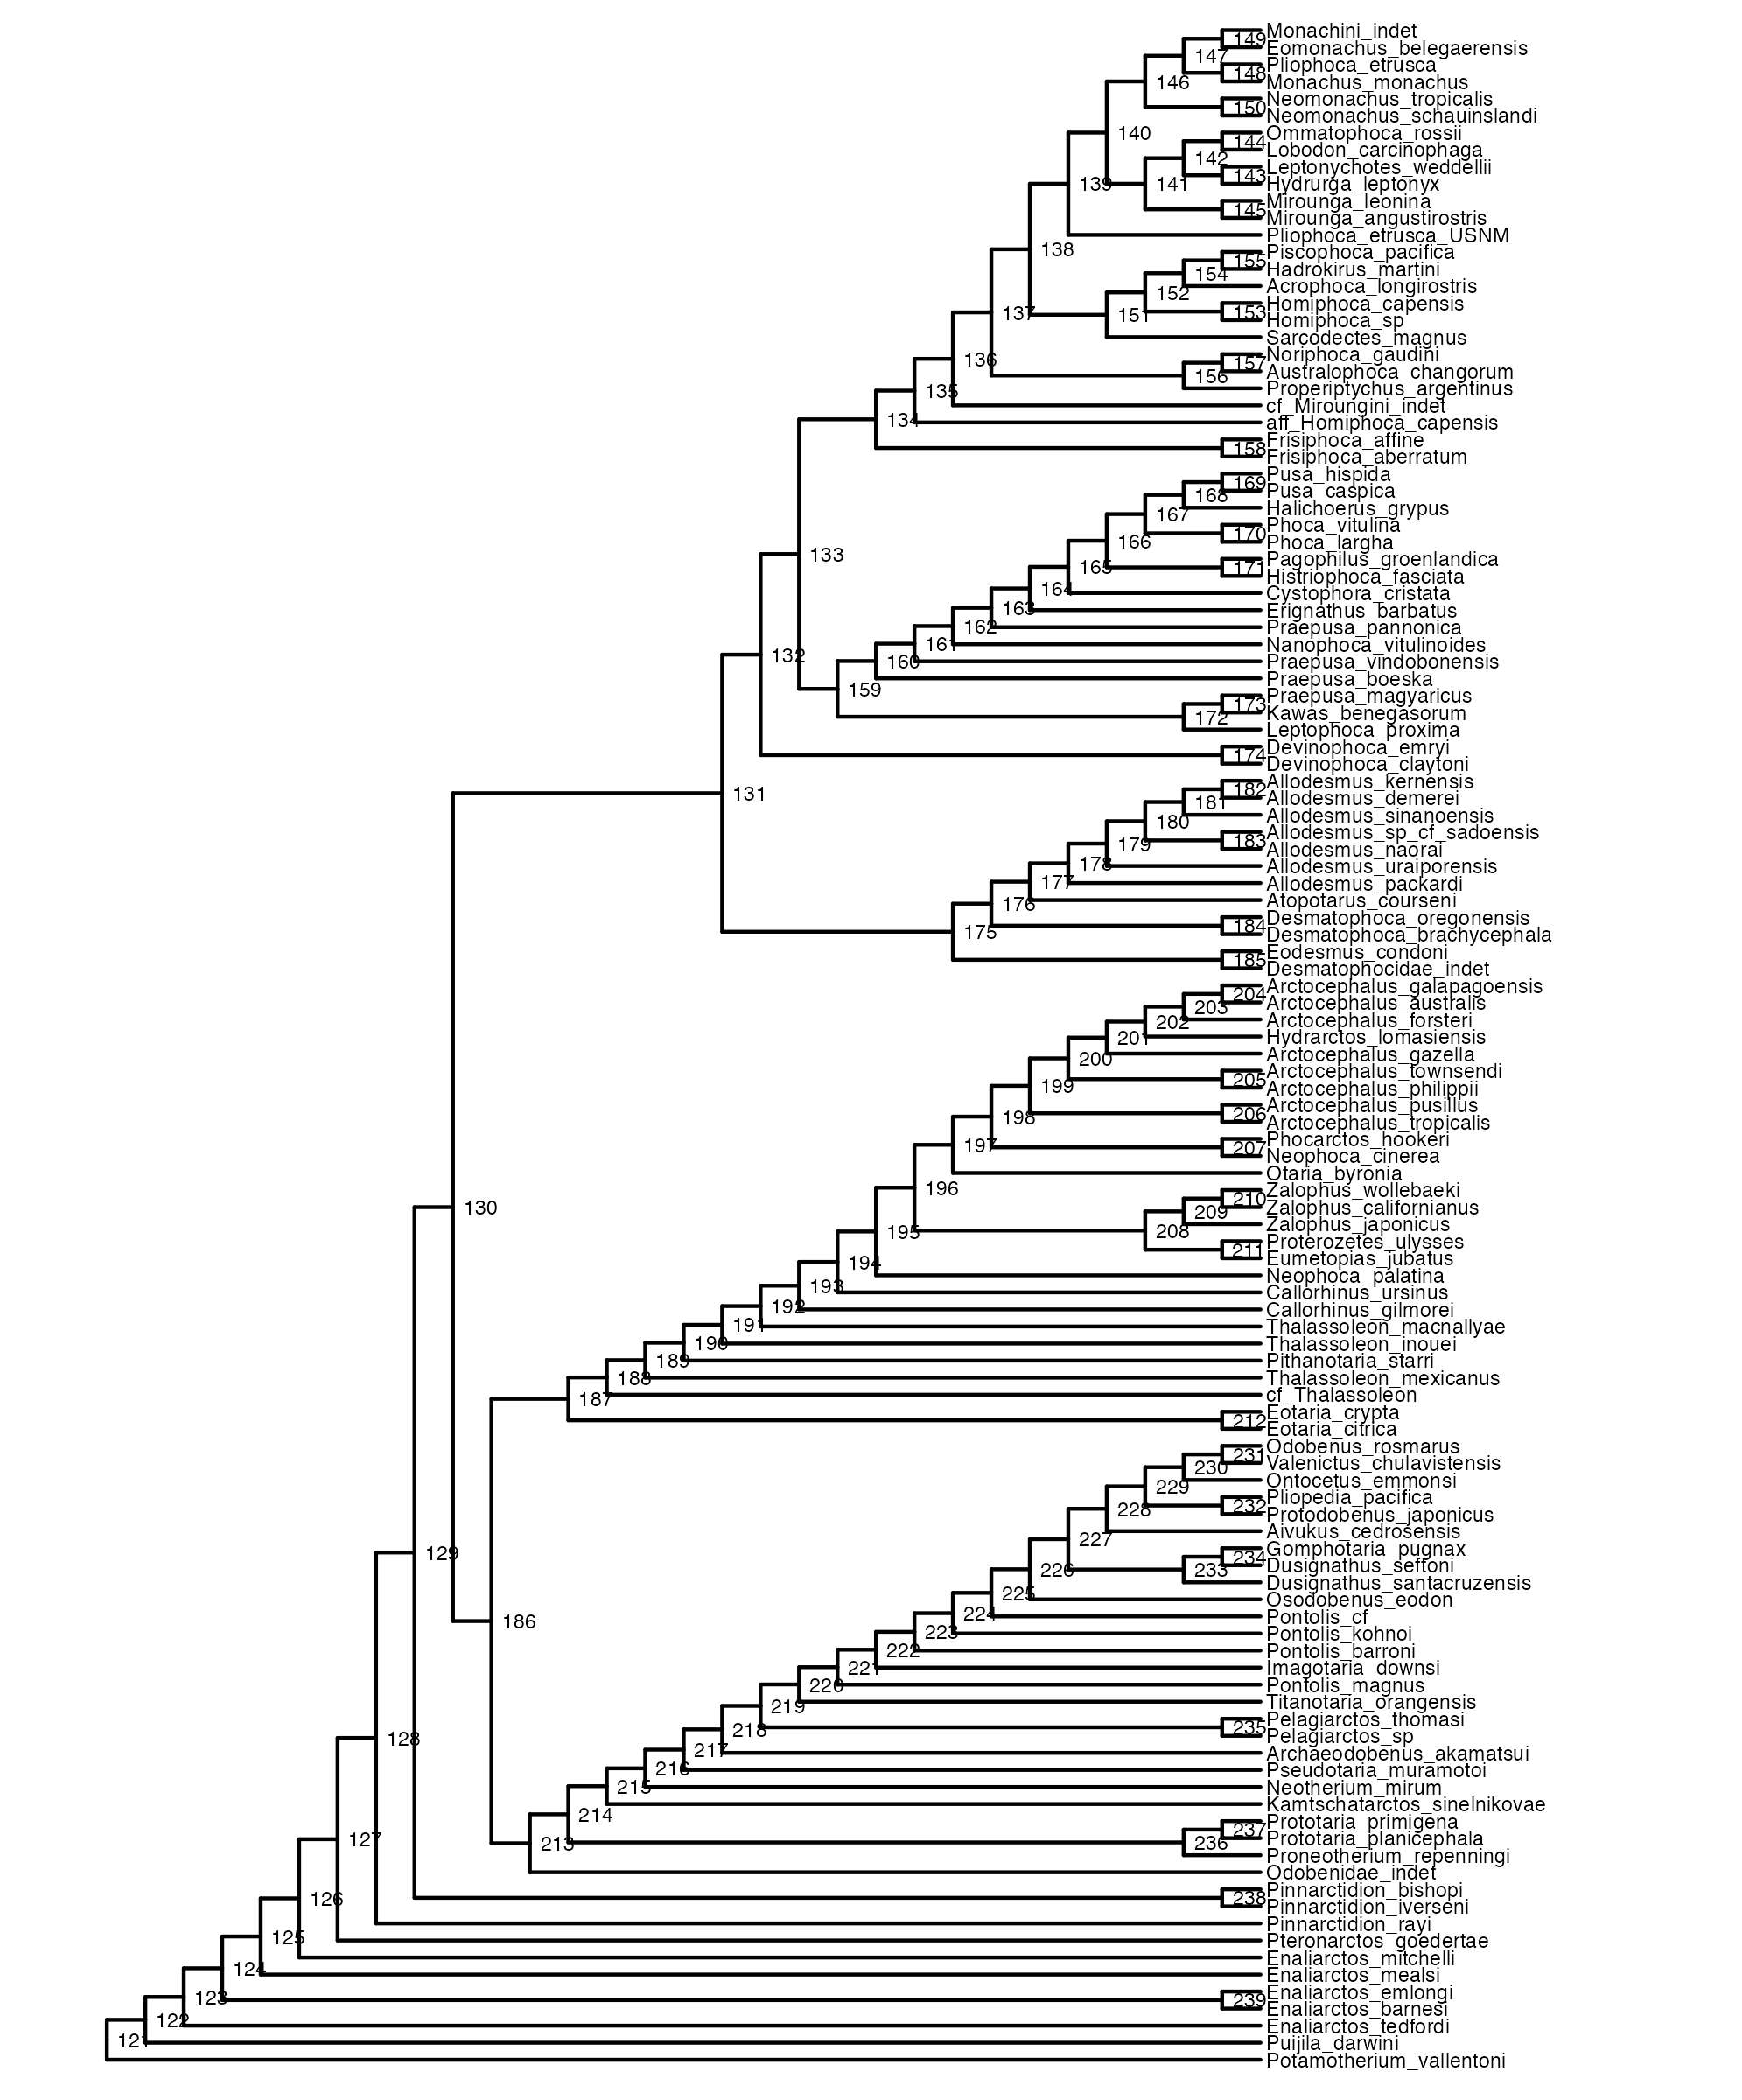
\includegraphics[width = \linewidth]{figures/node-labels-tree.png}
  \caption{Tree with node labels for help interpreting the full marginal probabilities at nodes results.}
  \label{fig-node-labels}
\end{figure}  

%-----------------------------------------------------------------------------------
\subsection{Detailed BioGeoBEARS outputs}

The plots below show the detailed results from the BioGeoBEARS analyses \citep{matzke2013probabilistic}. Models are either the dispersal-extinction-cladogenesis (DEC) model \citep{ree2008maximum} or the DEC+J model \citep{matzke2014model}. 
The nine different areas used were: (A) Northern Pacific Ocean, (B) Eastern South Pacific Ocean, (C) Australasian coastal waters, (D) Northern Atlantic Ocean, (E) Southern Atlantic Ocean, (F) Indian Ocean, (G) Southern Ocean, (H) Arctic Ocean, and (I) Paratethys/Mediterranean Ocean. Note that we excluded \textit{Pusa sibirica} (Lake Baikal seal) because of their isolated biogeography (they are only found in Lake Baikal). 
Legends and taxon names have been removed from Figures \ref{fig-all-dec-ml}-\ref{fig-all-decj-pie-unlikely} for readability. 
A full legend is shown in Figure \ref{fig-legend} and taxon names are shown in Figure \ref{fig-all-tree}.

% figure
\begin{figure}[H]
 \centering
  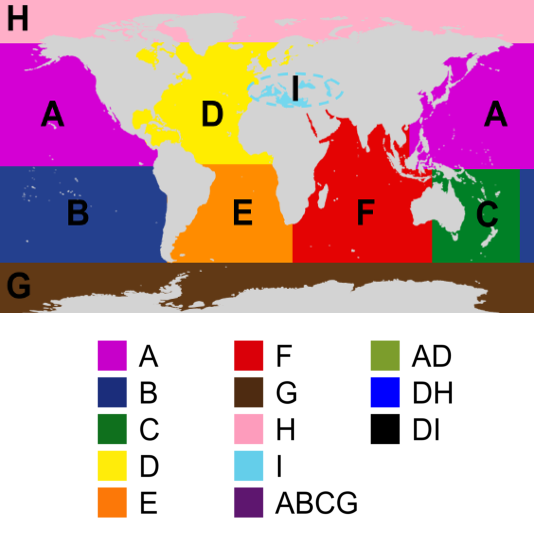
\includegraphics[width = 0.5\linewidth]{figures/BGB-legend.pdf}
  \caption{Legend for biogeography plots. The nine biogeographic areas used in our analyses are (A) Northern Pacific Ocean, (B) Eastern South Pacific Ocean, (C) Australasian coastal waters, (D) Northern Atlantic Ocean, (E) Southern Atlantic Ocean, (F) Indian Ocean, (G) Southern Ocean, (H) Arctic Ocean, and (I) Paratethys/Mediterranean Ocean. Colours for states representing more than one area found at the nodes of the phylogeny (ABCG, AD, DH, DI) are also shown.}
  \label{fig-legend}
\end{figure} 

\subsubsection{Impossible states removed}

% figure
\begin{figure}[H]
 \centering
  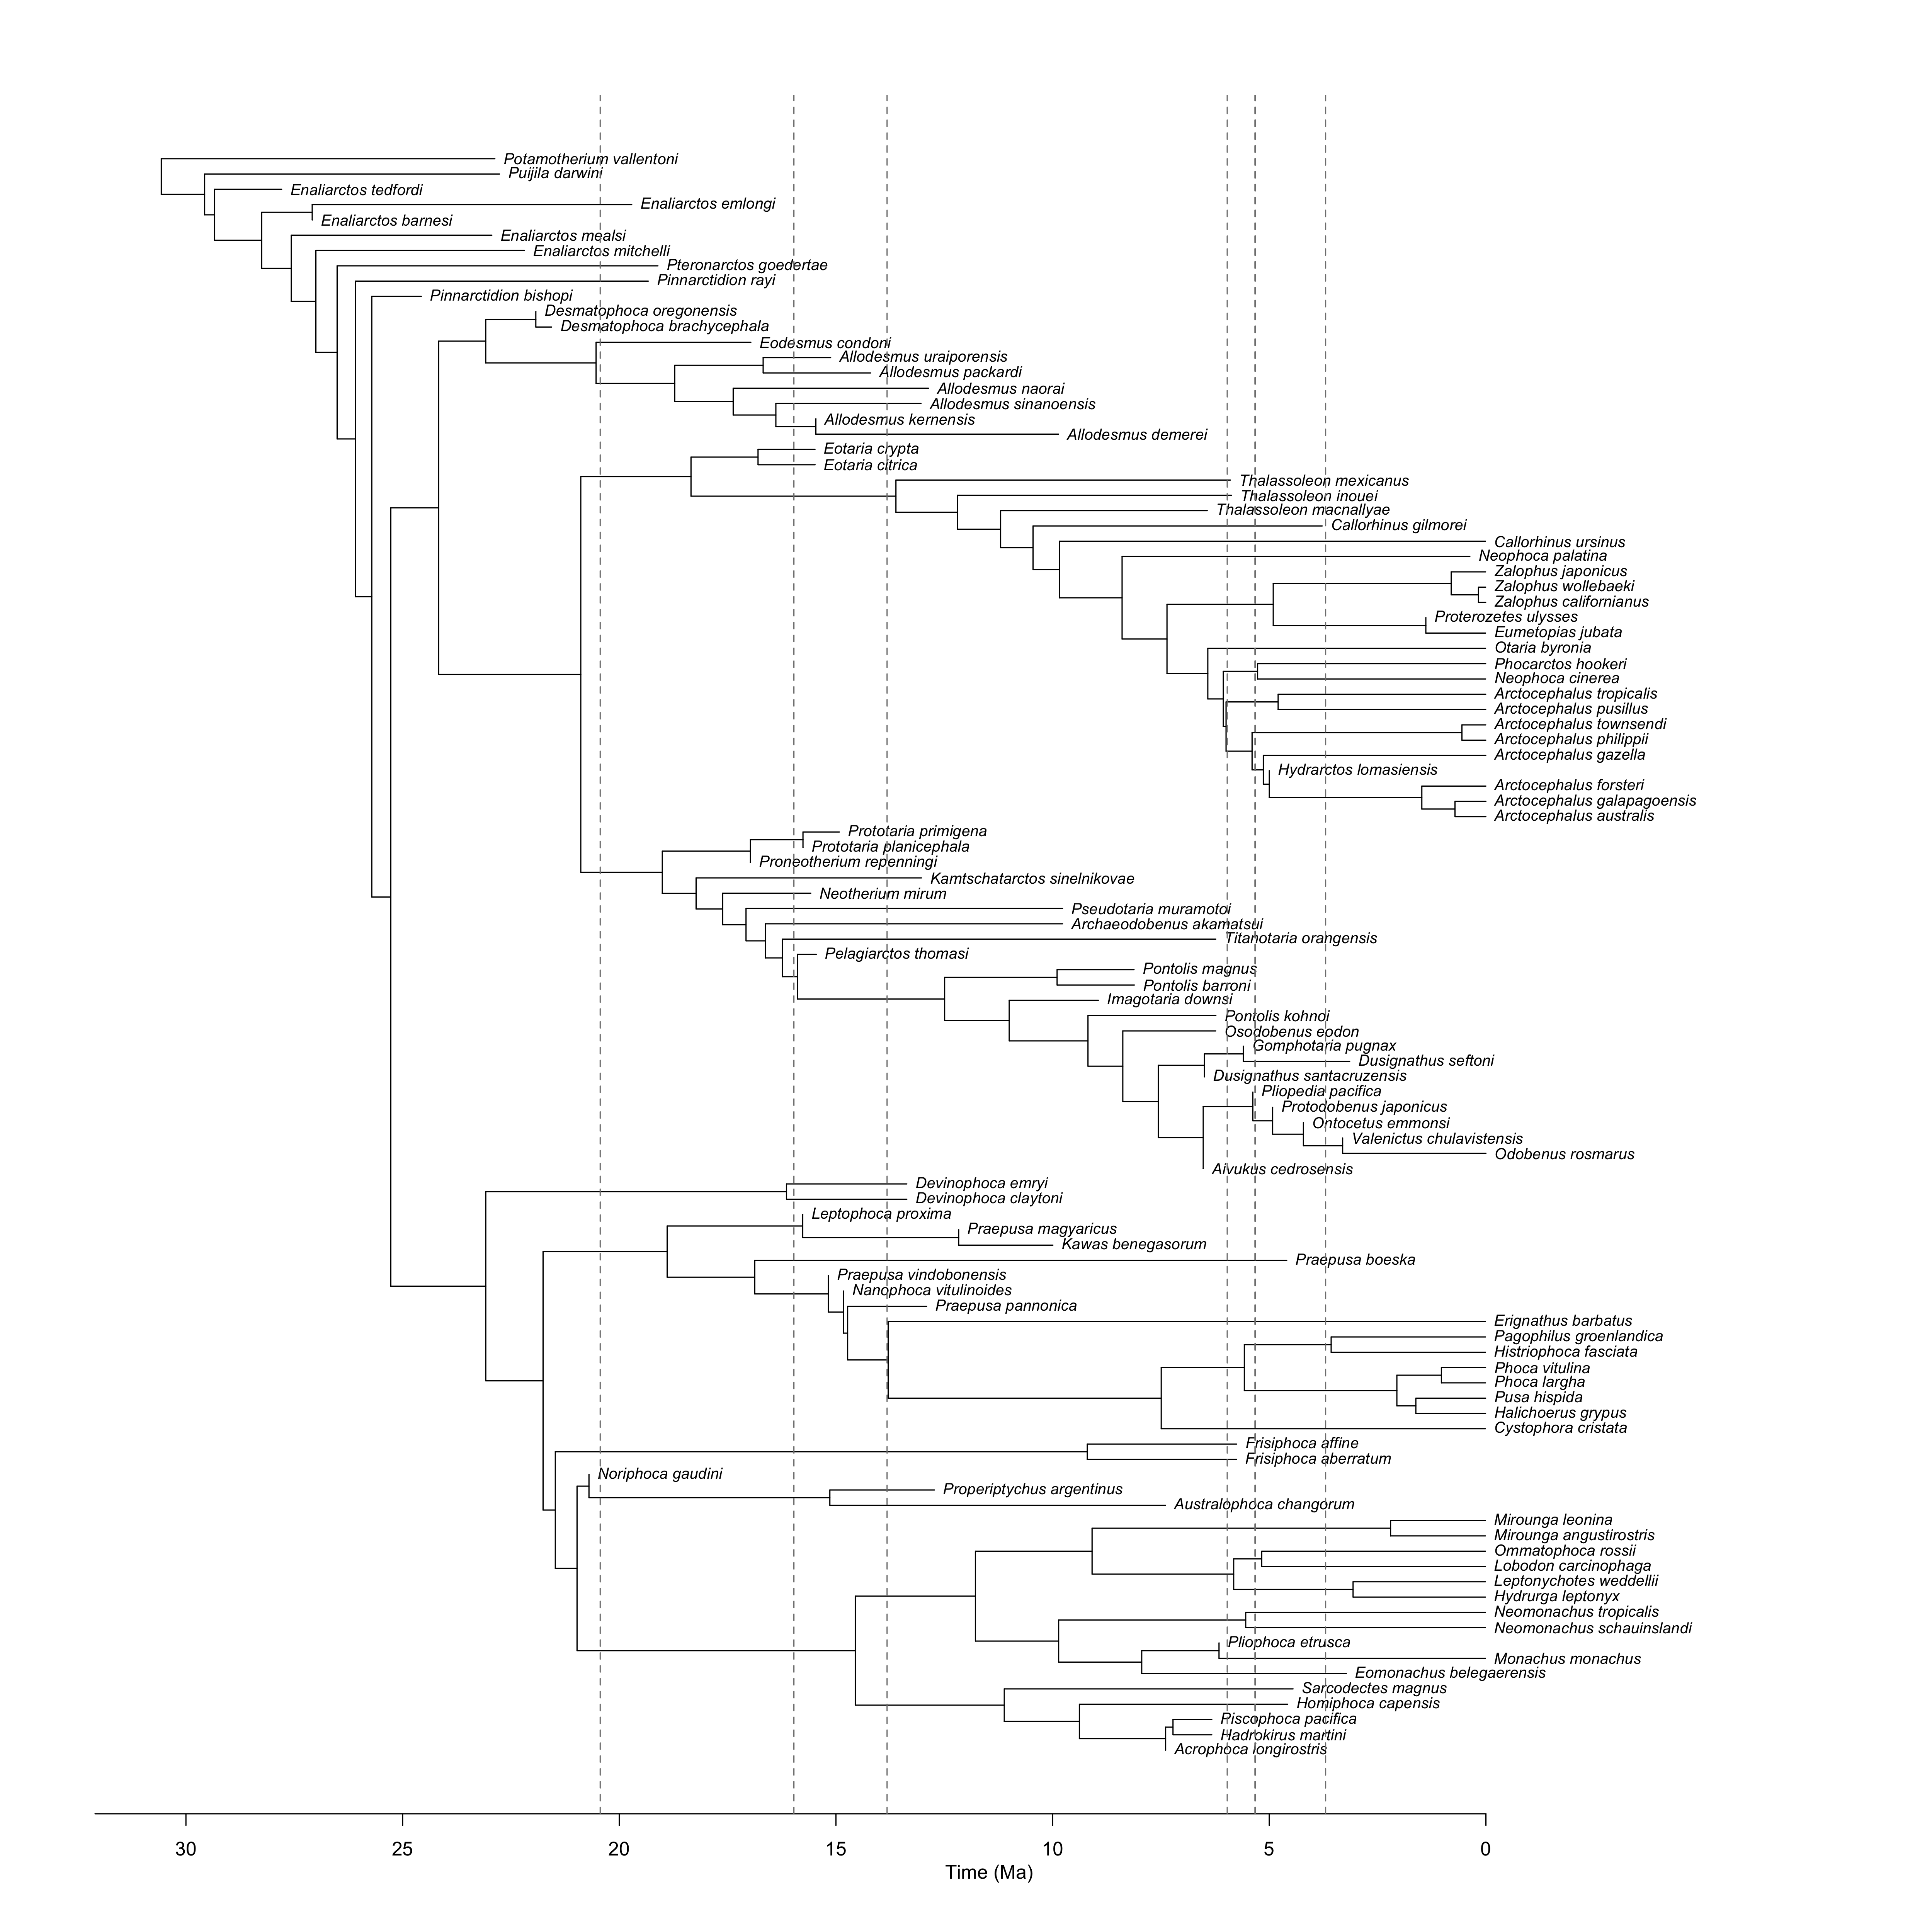
\includegraphics[width = \linewidth]{figures/all-pinnipeds-tree.png}
  \caption{Phylogeny of pinnipeds with taxon names to aid understanding of the following results which have taxon names removed to improve readability.}
  \label{fig-all-tree}
\end{figure} 

% figure
\begin{figure}[H]
 \centering
  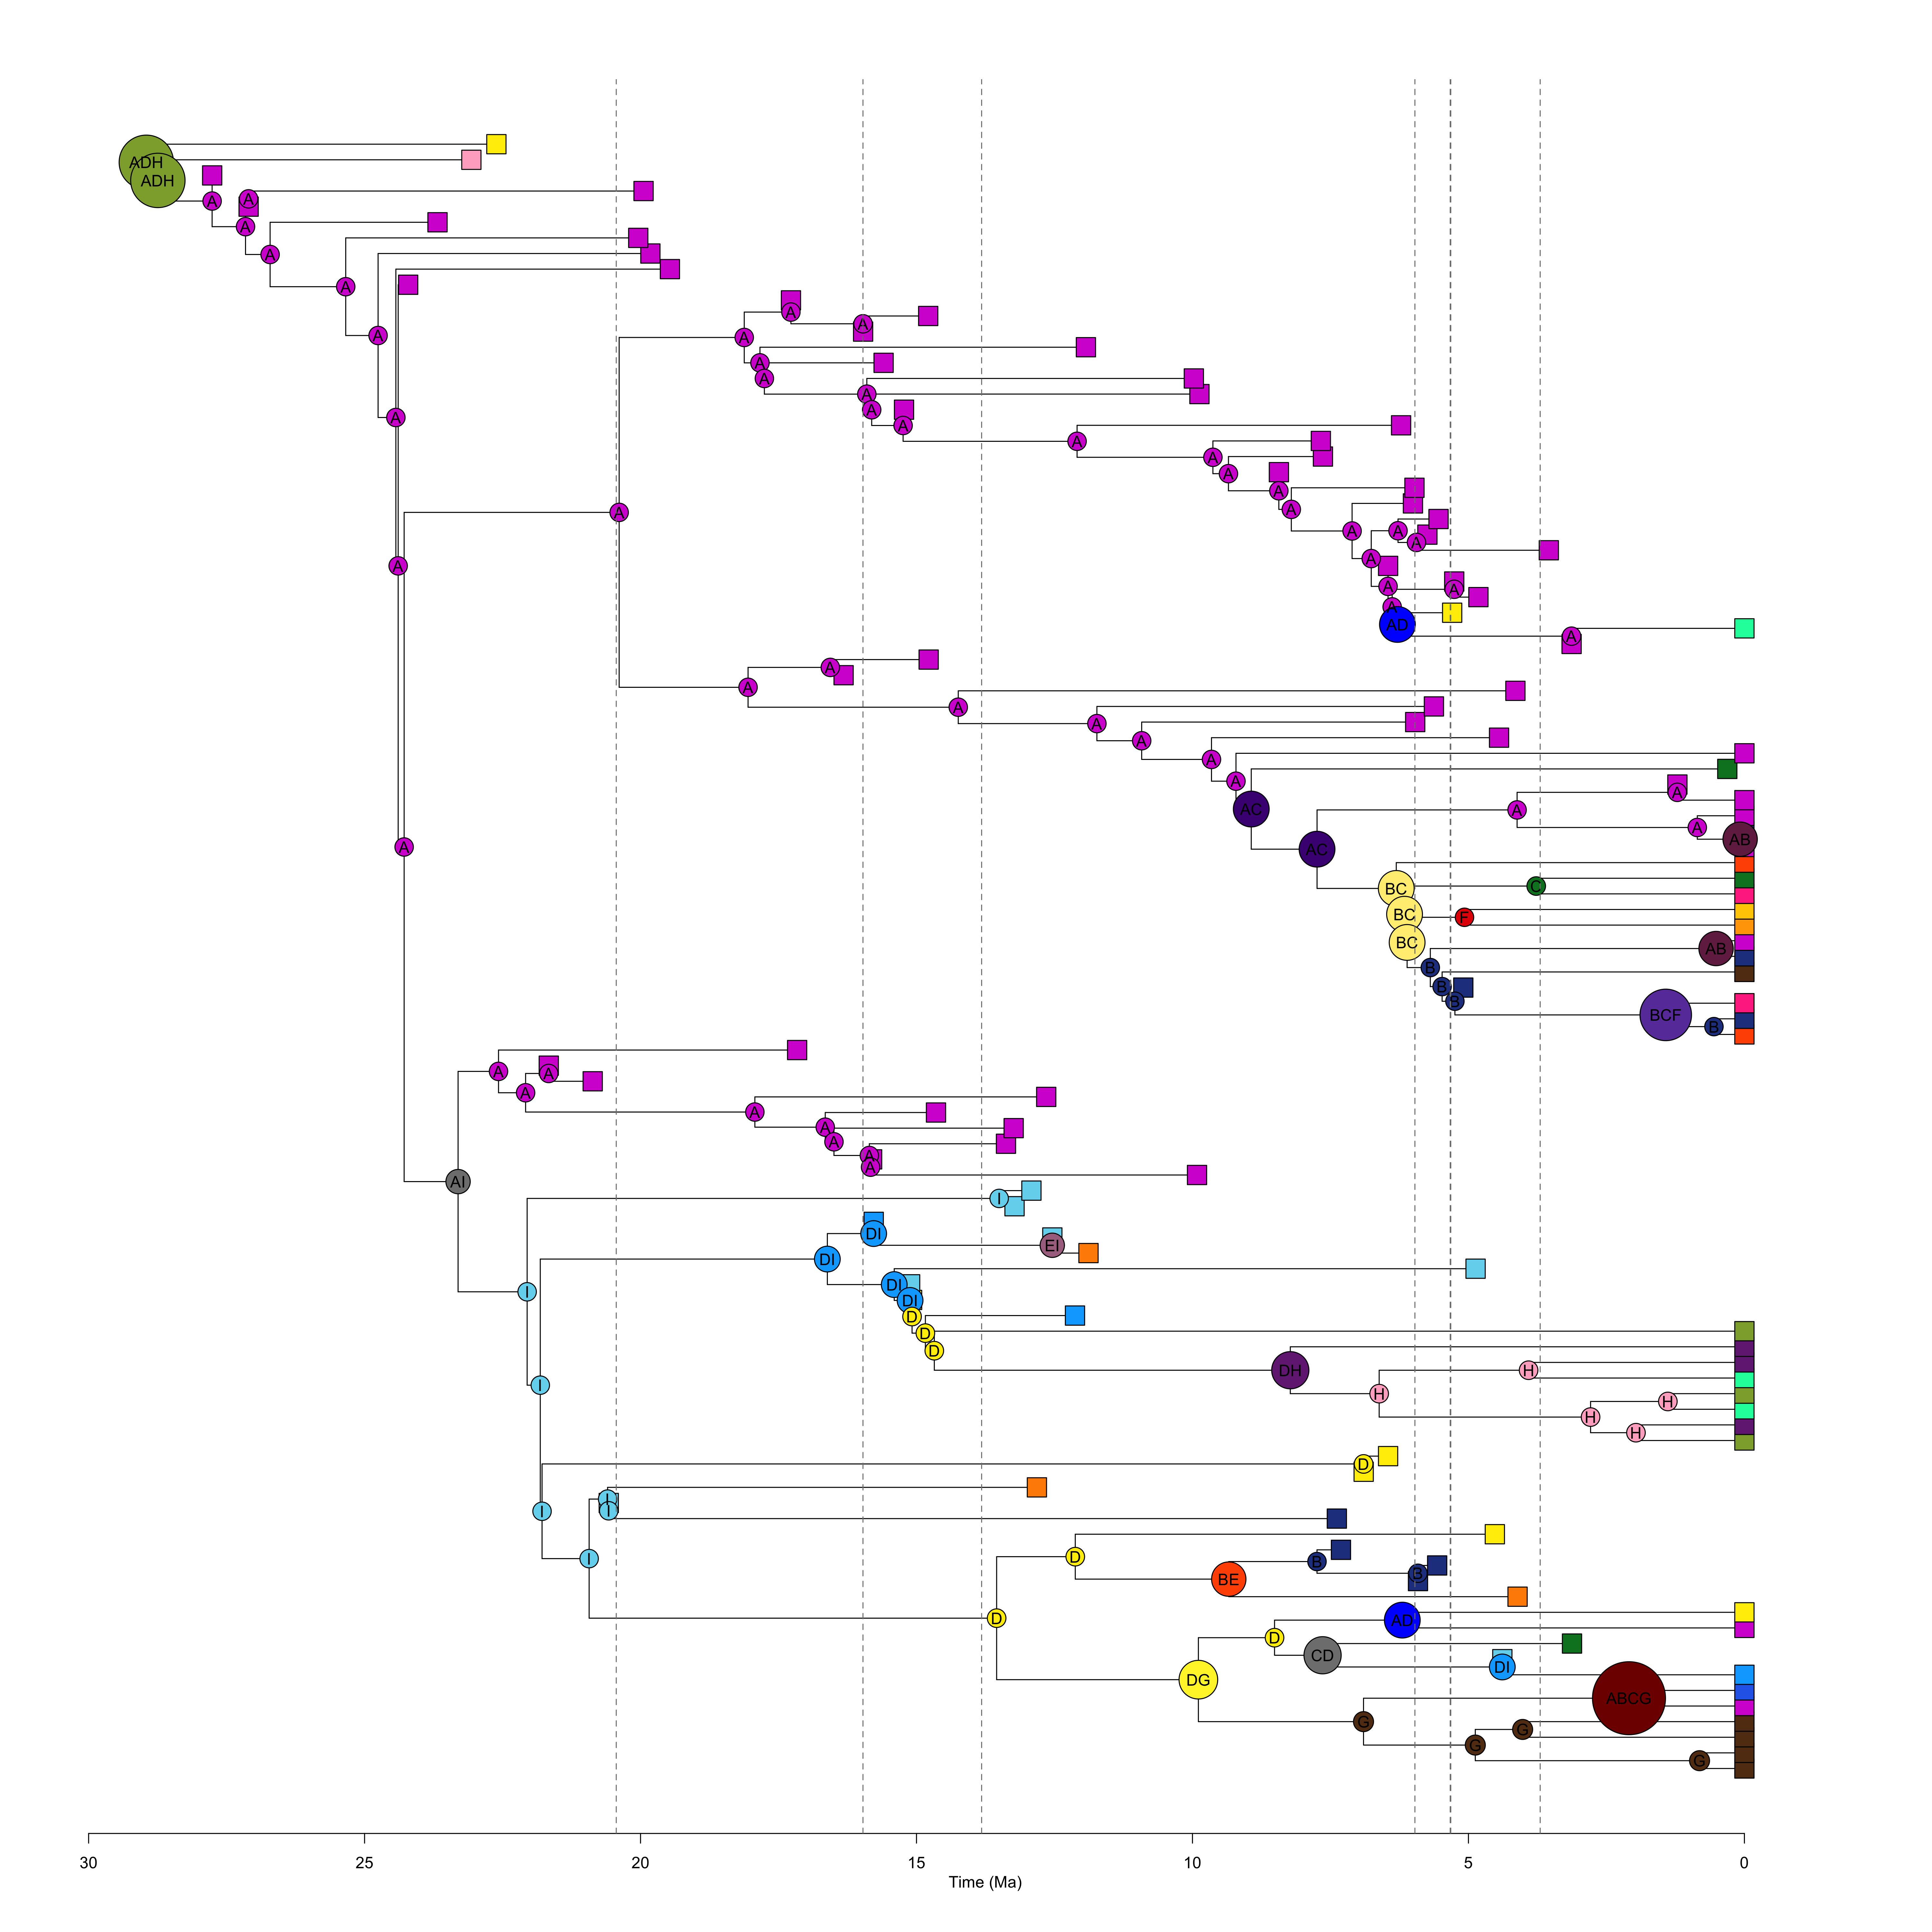
\includegraphics[width = \linewidth]{figures/all-pinnipeds-DEC-impossible-MLstates.png}
  \caption{DEC model, impossible states removed. Nodes show Maximum Likelihood states.}
  \label{fig-all-dec-ml}
\end{figure} 

% figure
\begin{figure}[H]
 \centering
  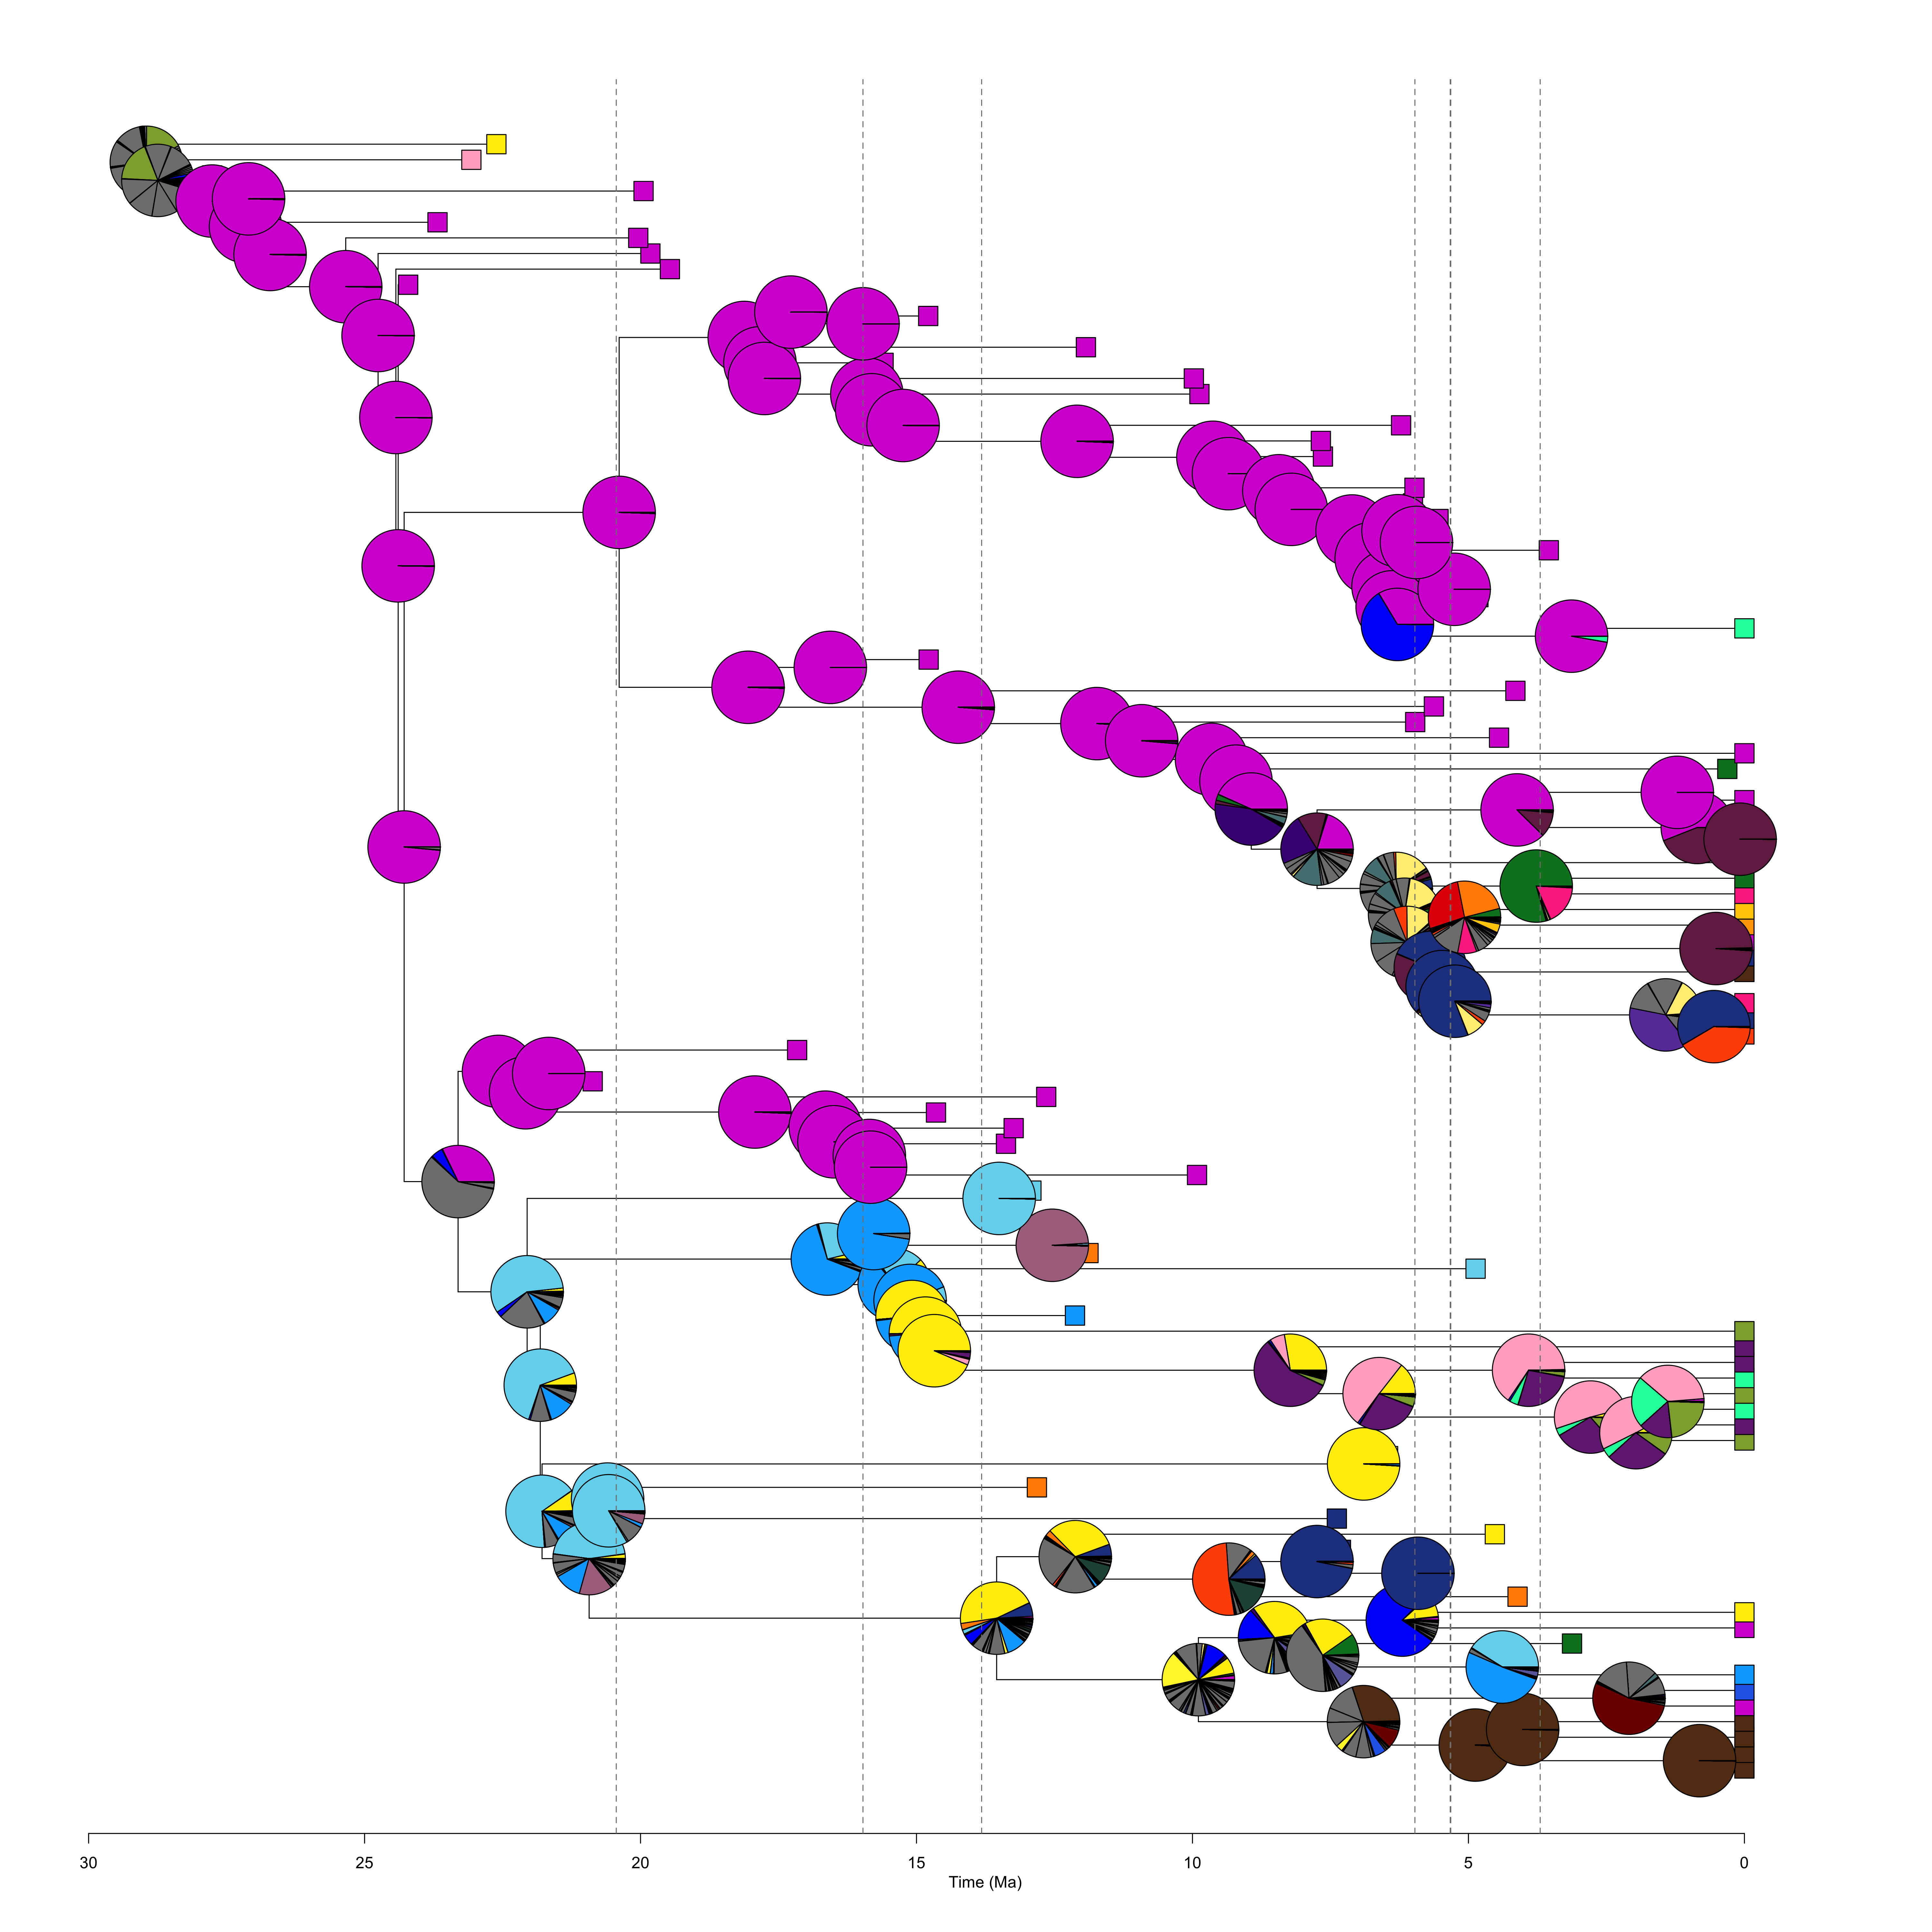
\includegraphics[width = \linewidth]{figures/all-pinnipeds-DEC-impossible-pies.png}
  \caption{DEC model, impossible states removed. Nodes show relative probabilities of each state.}
  \label{fig-all-dec-pie}
\end{figure} 

% figure
\begin{figure}[H]
 \centering
  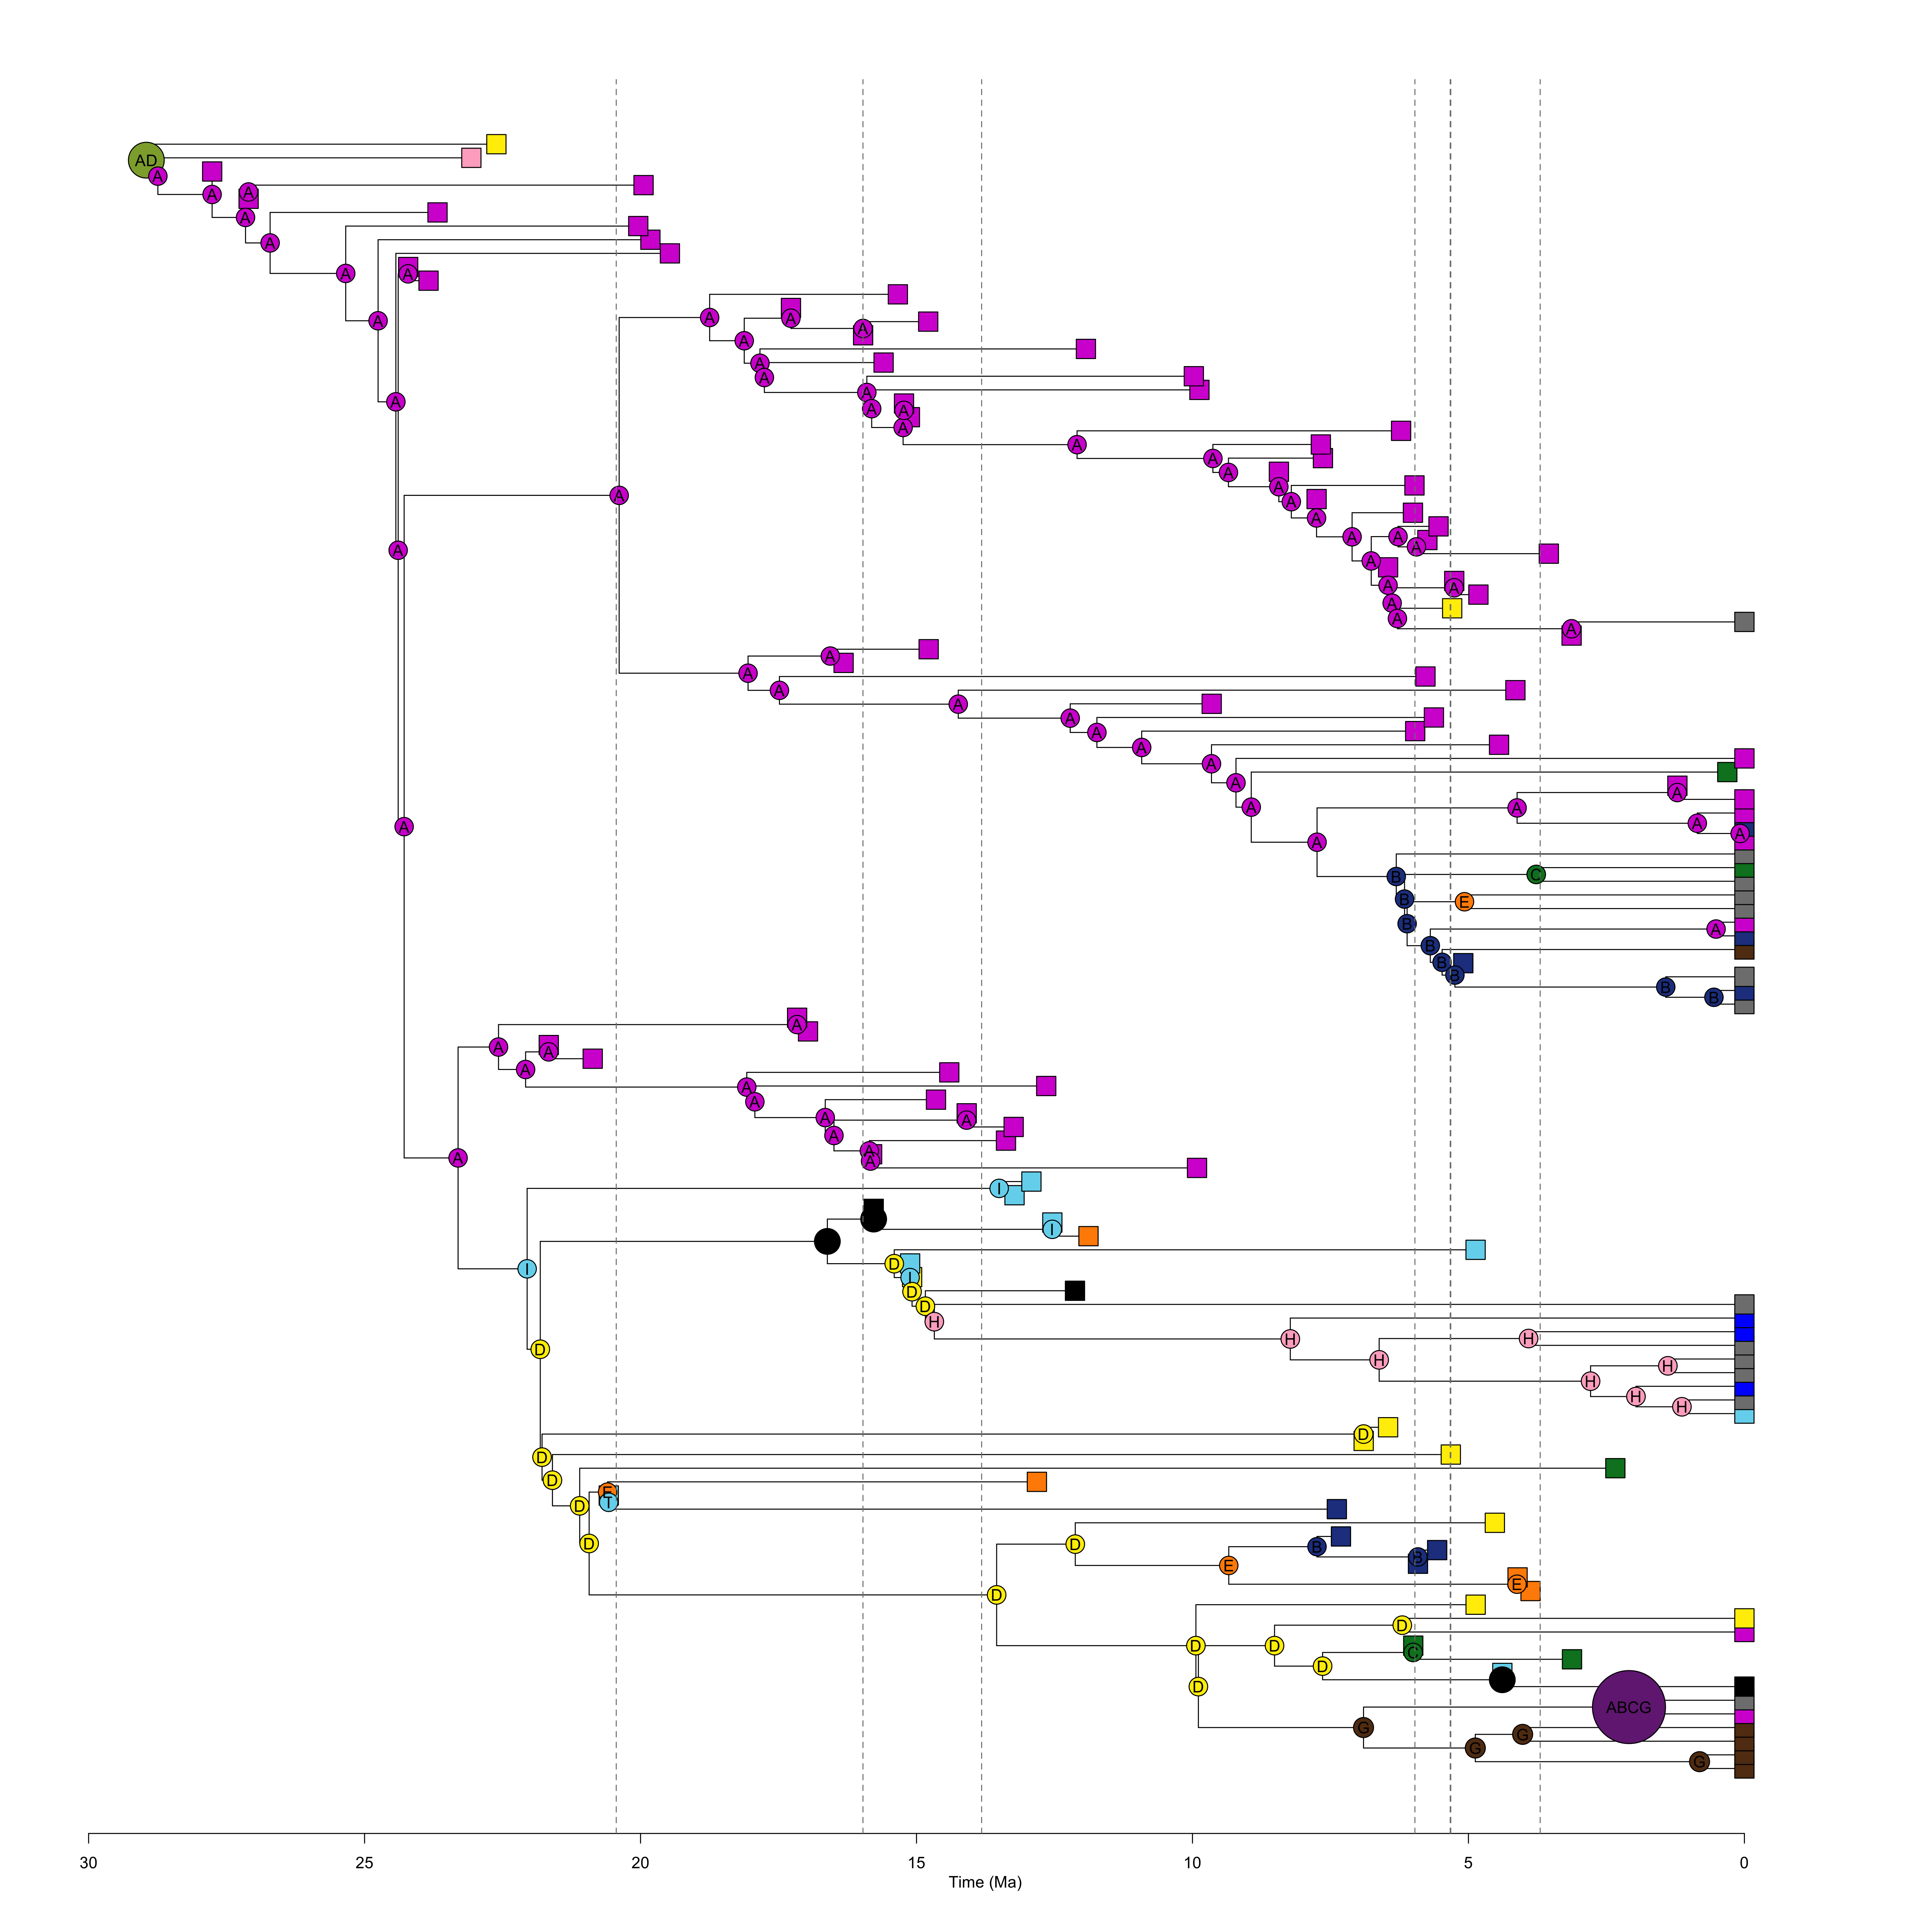
\includegraphics[width = \linewidth]{figures/all-pinnipeds-DECj-impossible-MLstates.png}
  \caption{DEC+J model, impossible states removed. Nodes show Maximum Likelihood states.}
  \label{fig-all-decj-ml}
\end{figure} 

% figure
\begin{figure}[H]
 \centering
  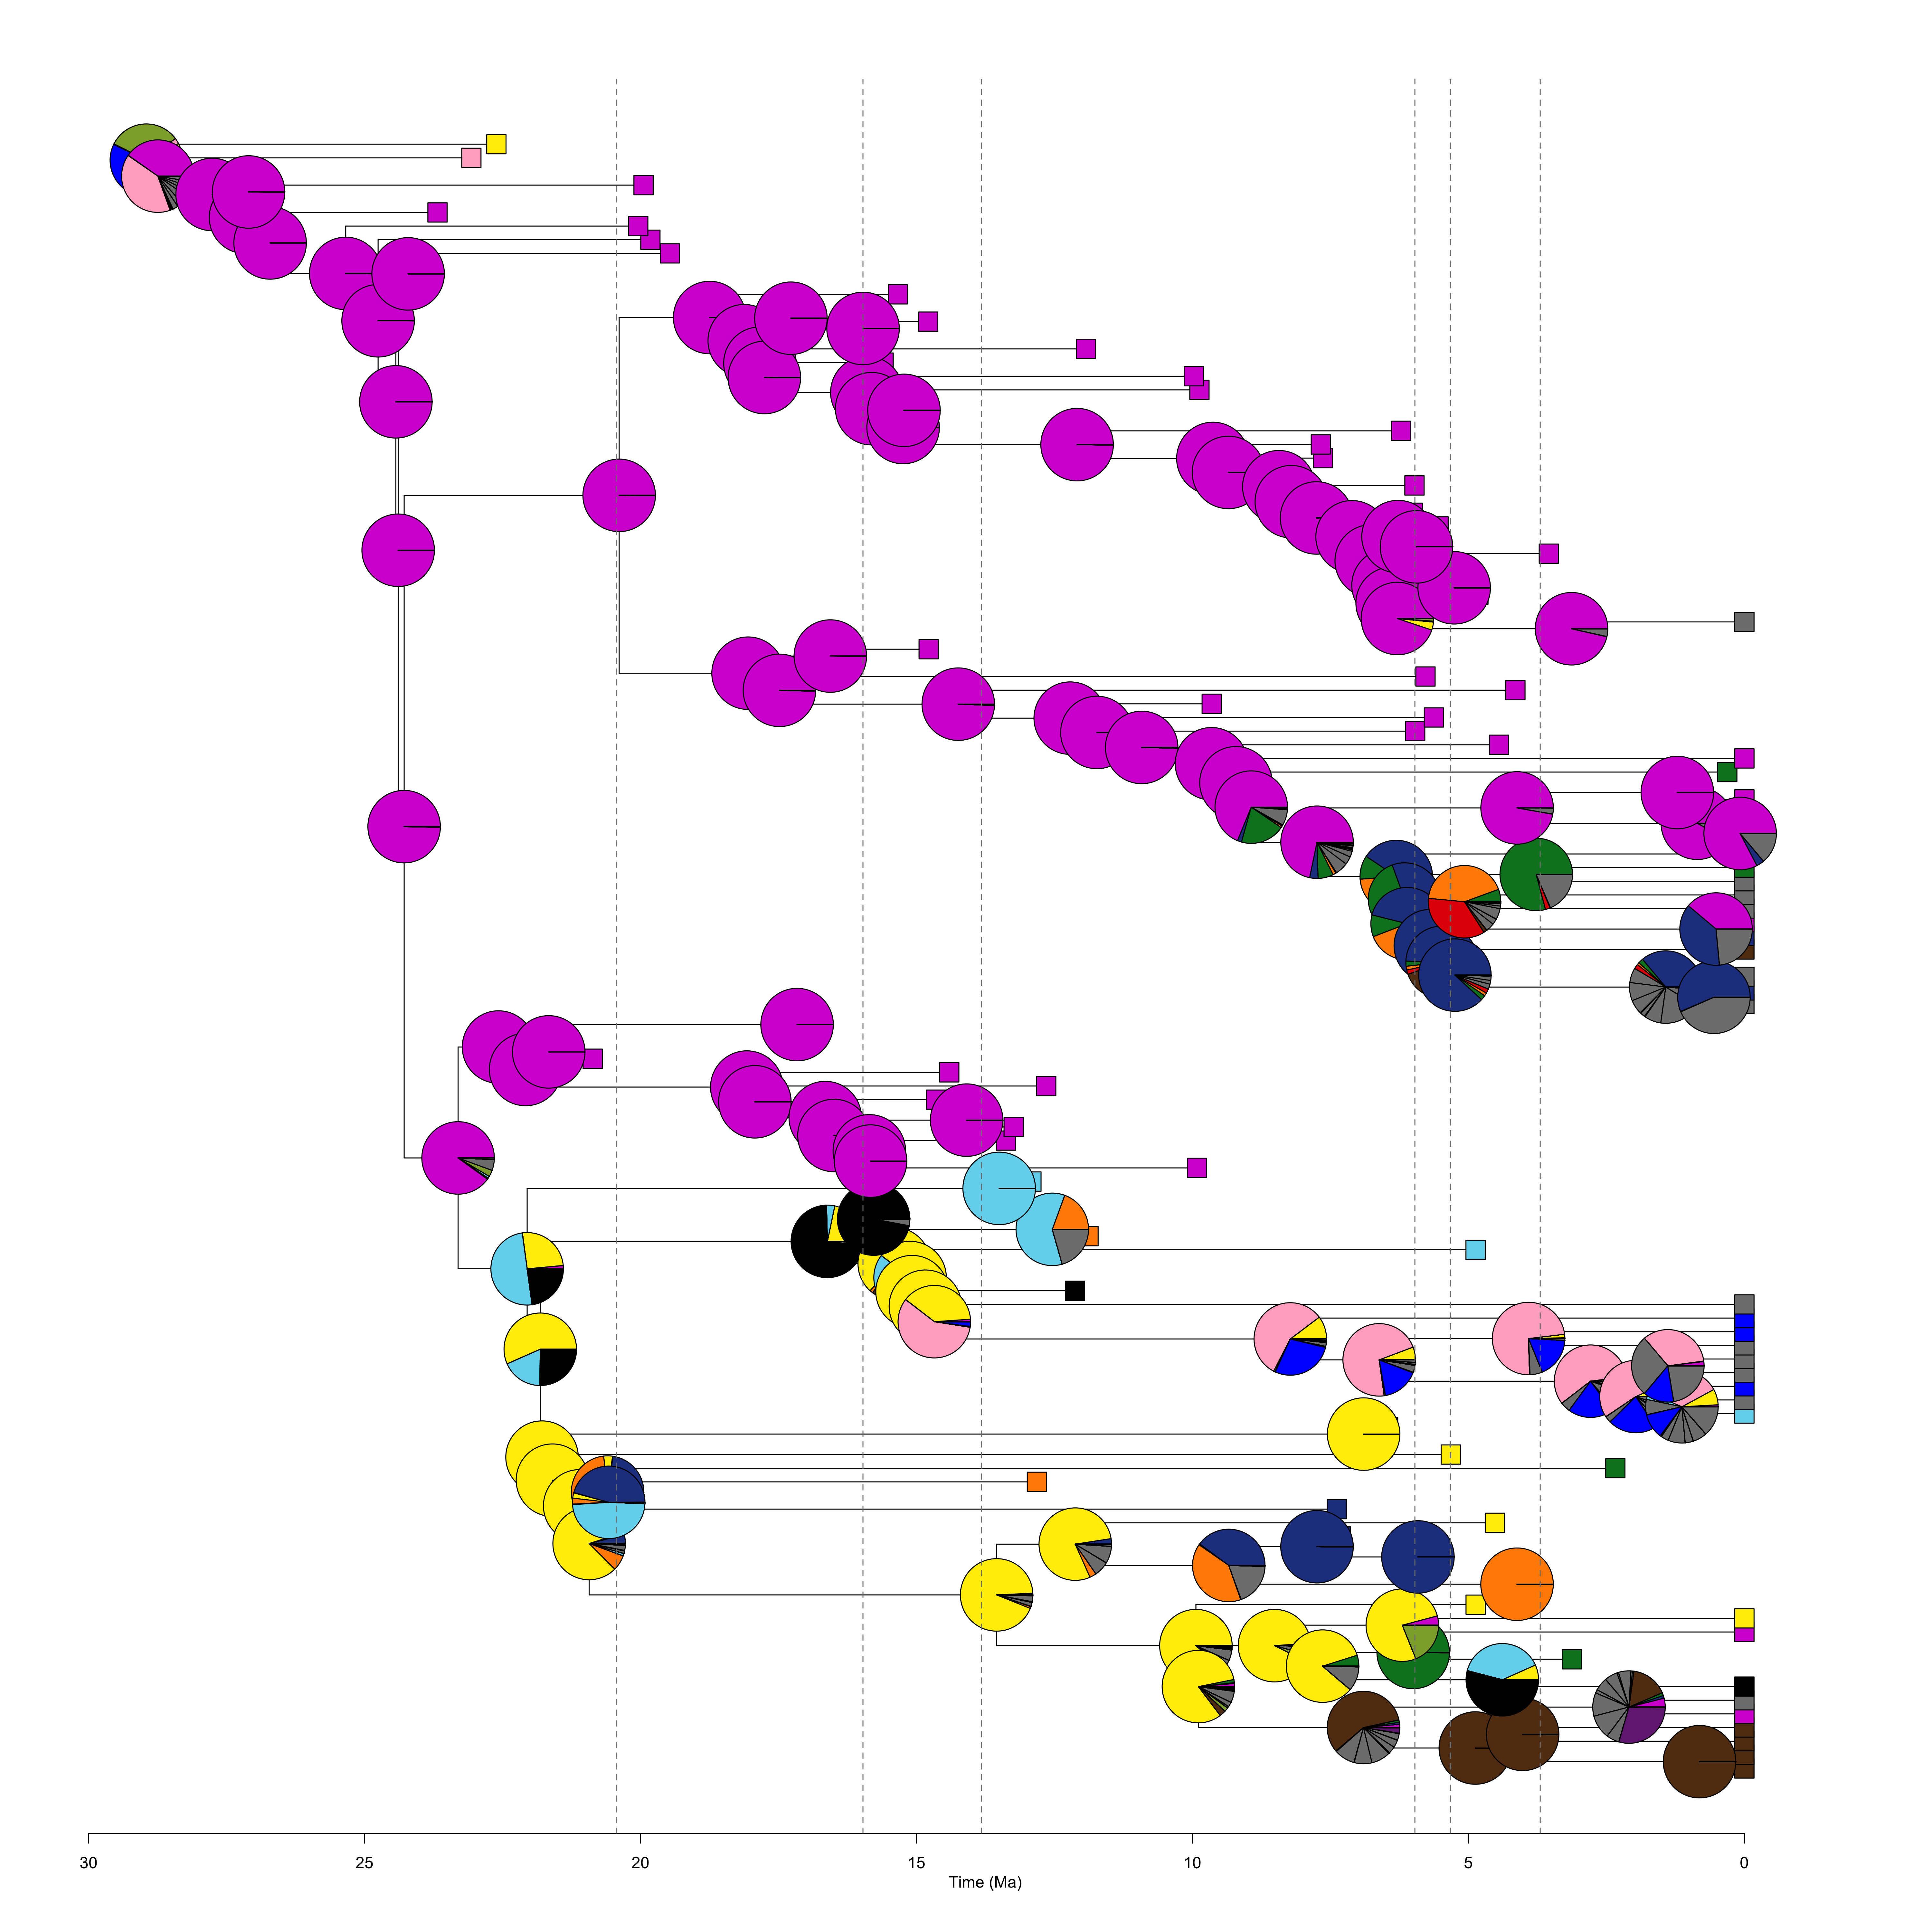
\includegraphics[width = \linewidth]{figures/all-pinnipeds-DECj-impossible-pies.png}
  \caption{DEC+J model, impossible states removed. Nodes show relative probabilities of each state.}
  \label{fig-all-decj-pie}
\end{figure} 
 
%-----------------------------------------------------------------------------------
% unlikely

\subsubsection{Impossible and unlikely states removed}

% figure
\begin{figure}[H]
 \centering
  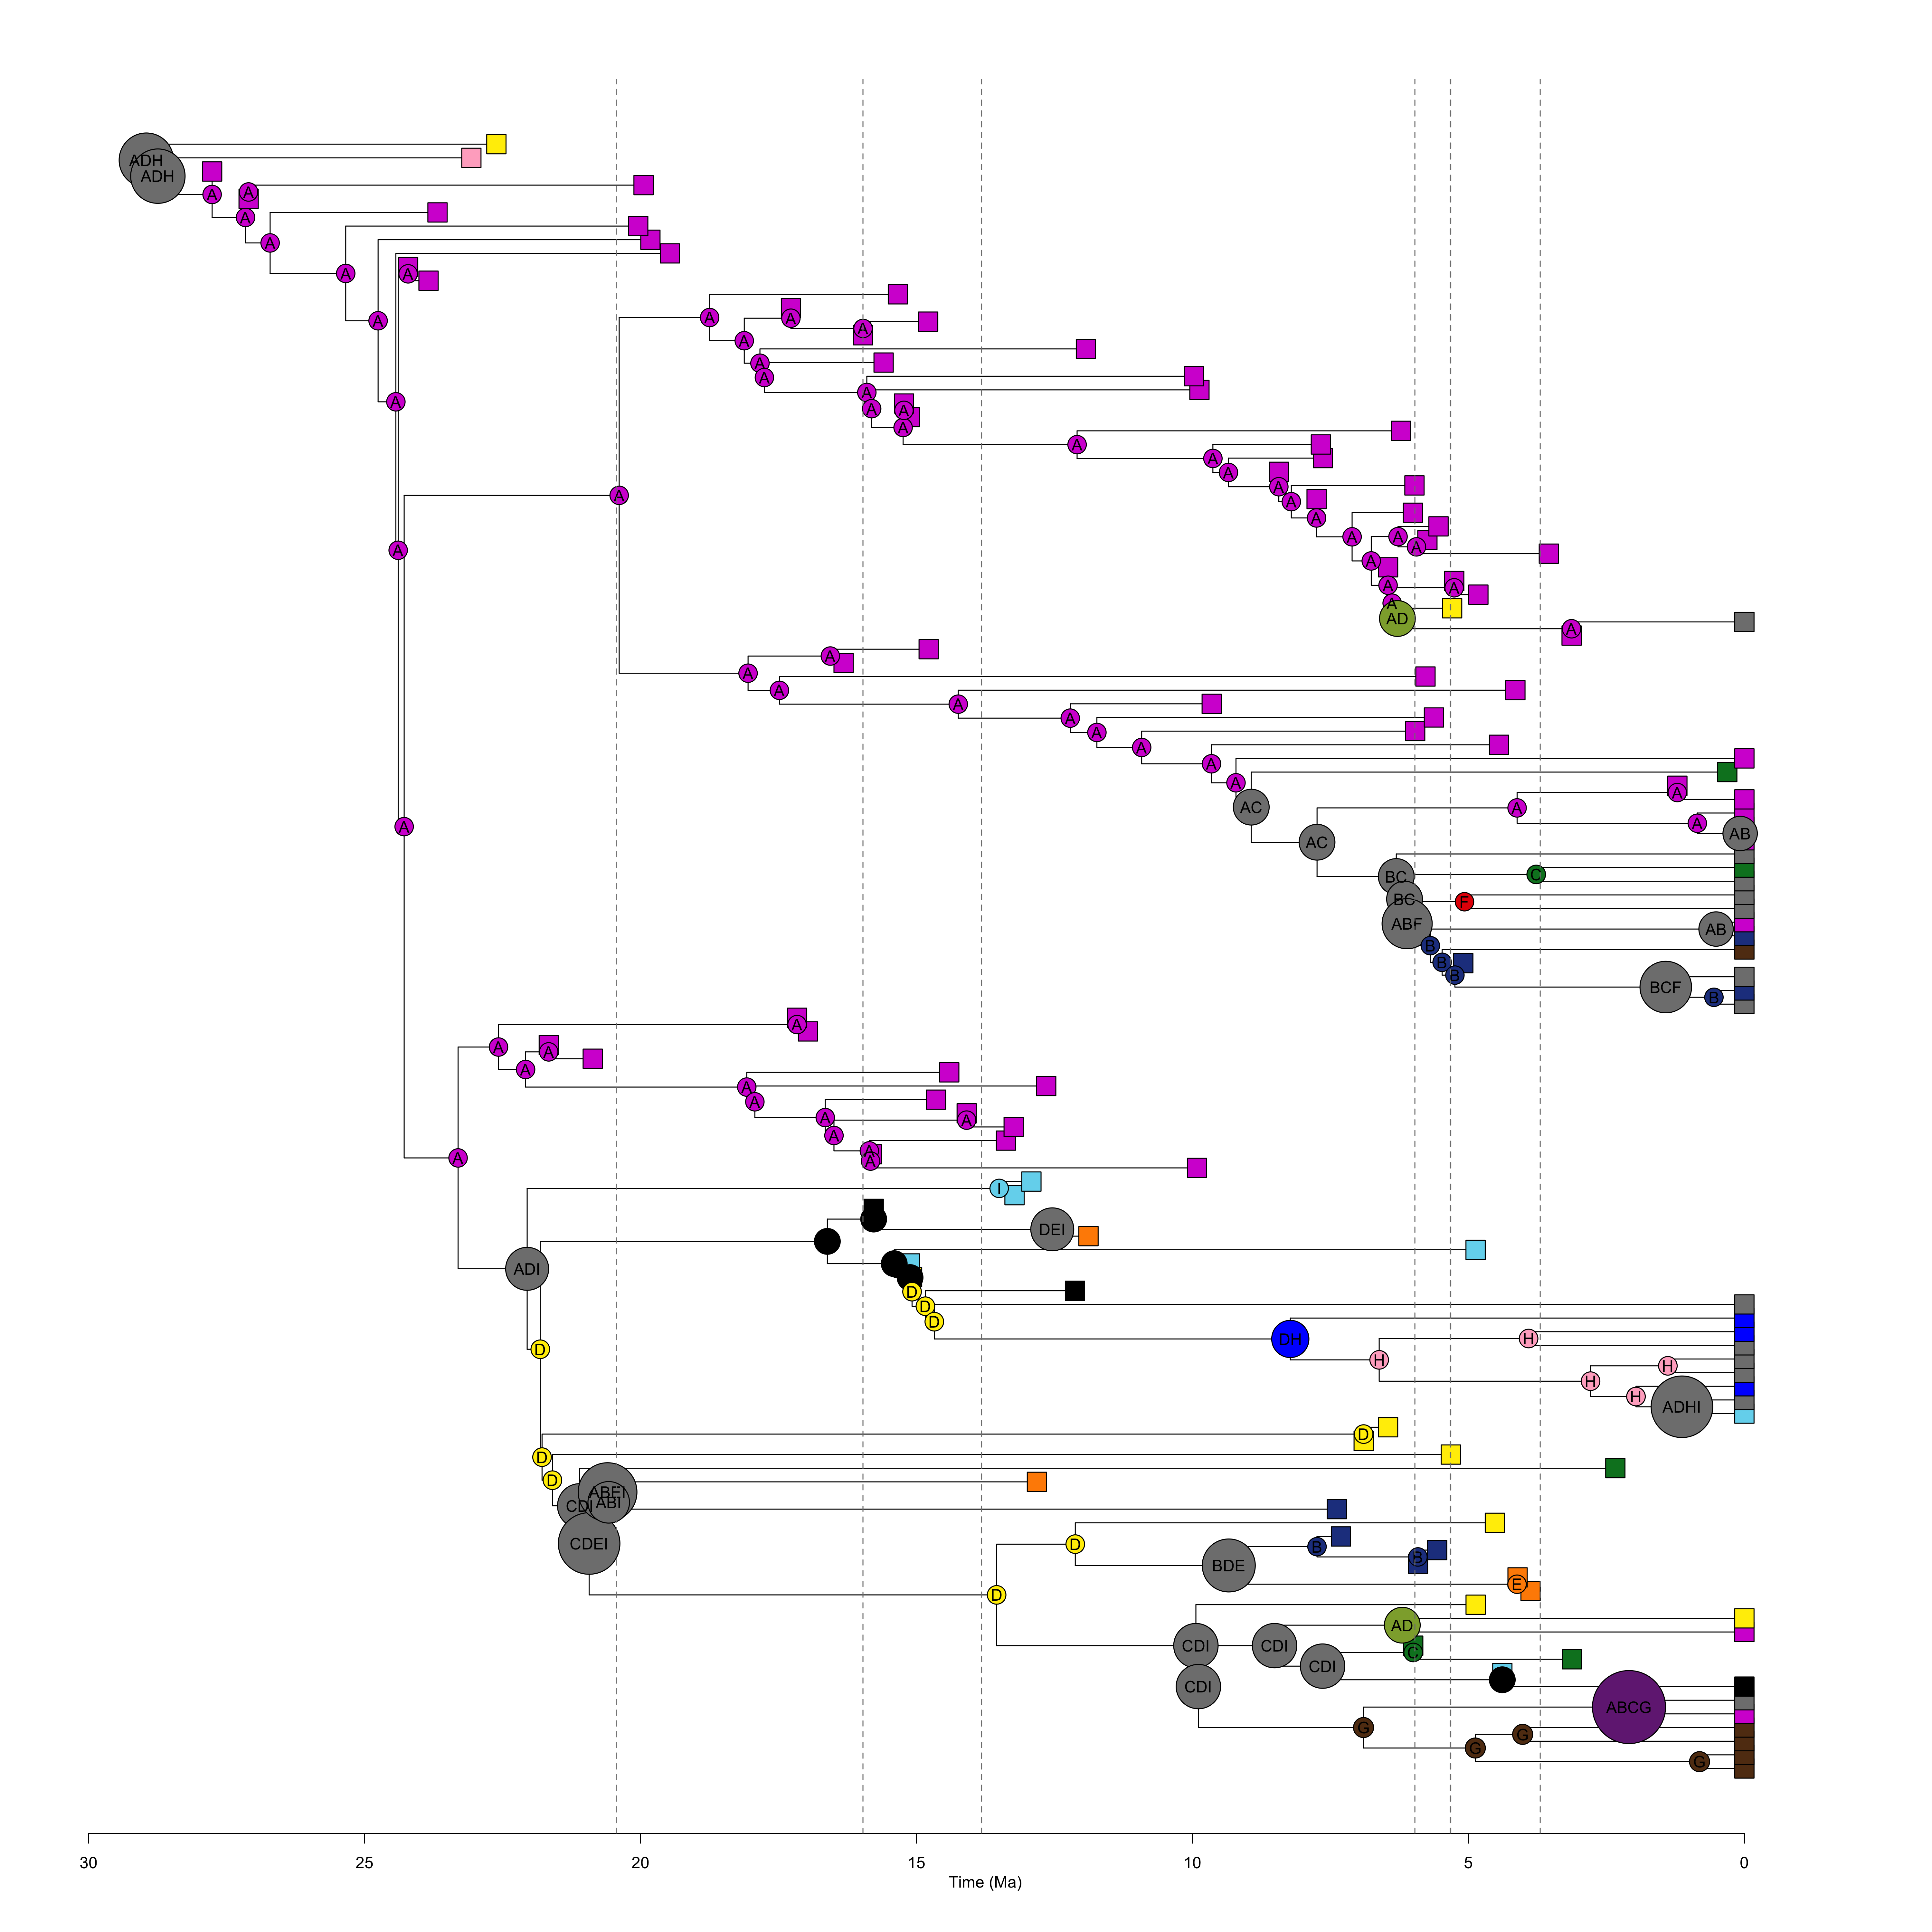
\includegraphics[width = \linewidth]{figures/all-pinnipeds-DEC-unlikely-MLstates.png}
  \caption{DEC model, impossible and unlikely states removed. Nodes show Maximum Likelihood states.}
  \label{fig-all-dec-ml-unlikely}
\end{figure} 

% figure
\begin{figure}[H]
 \centering
  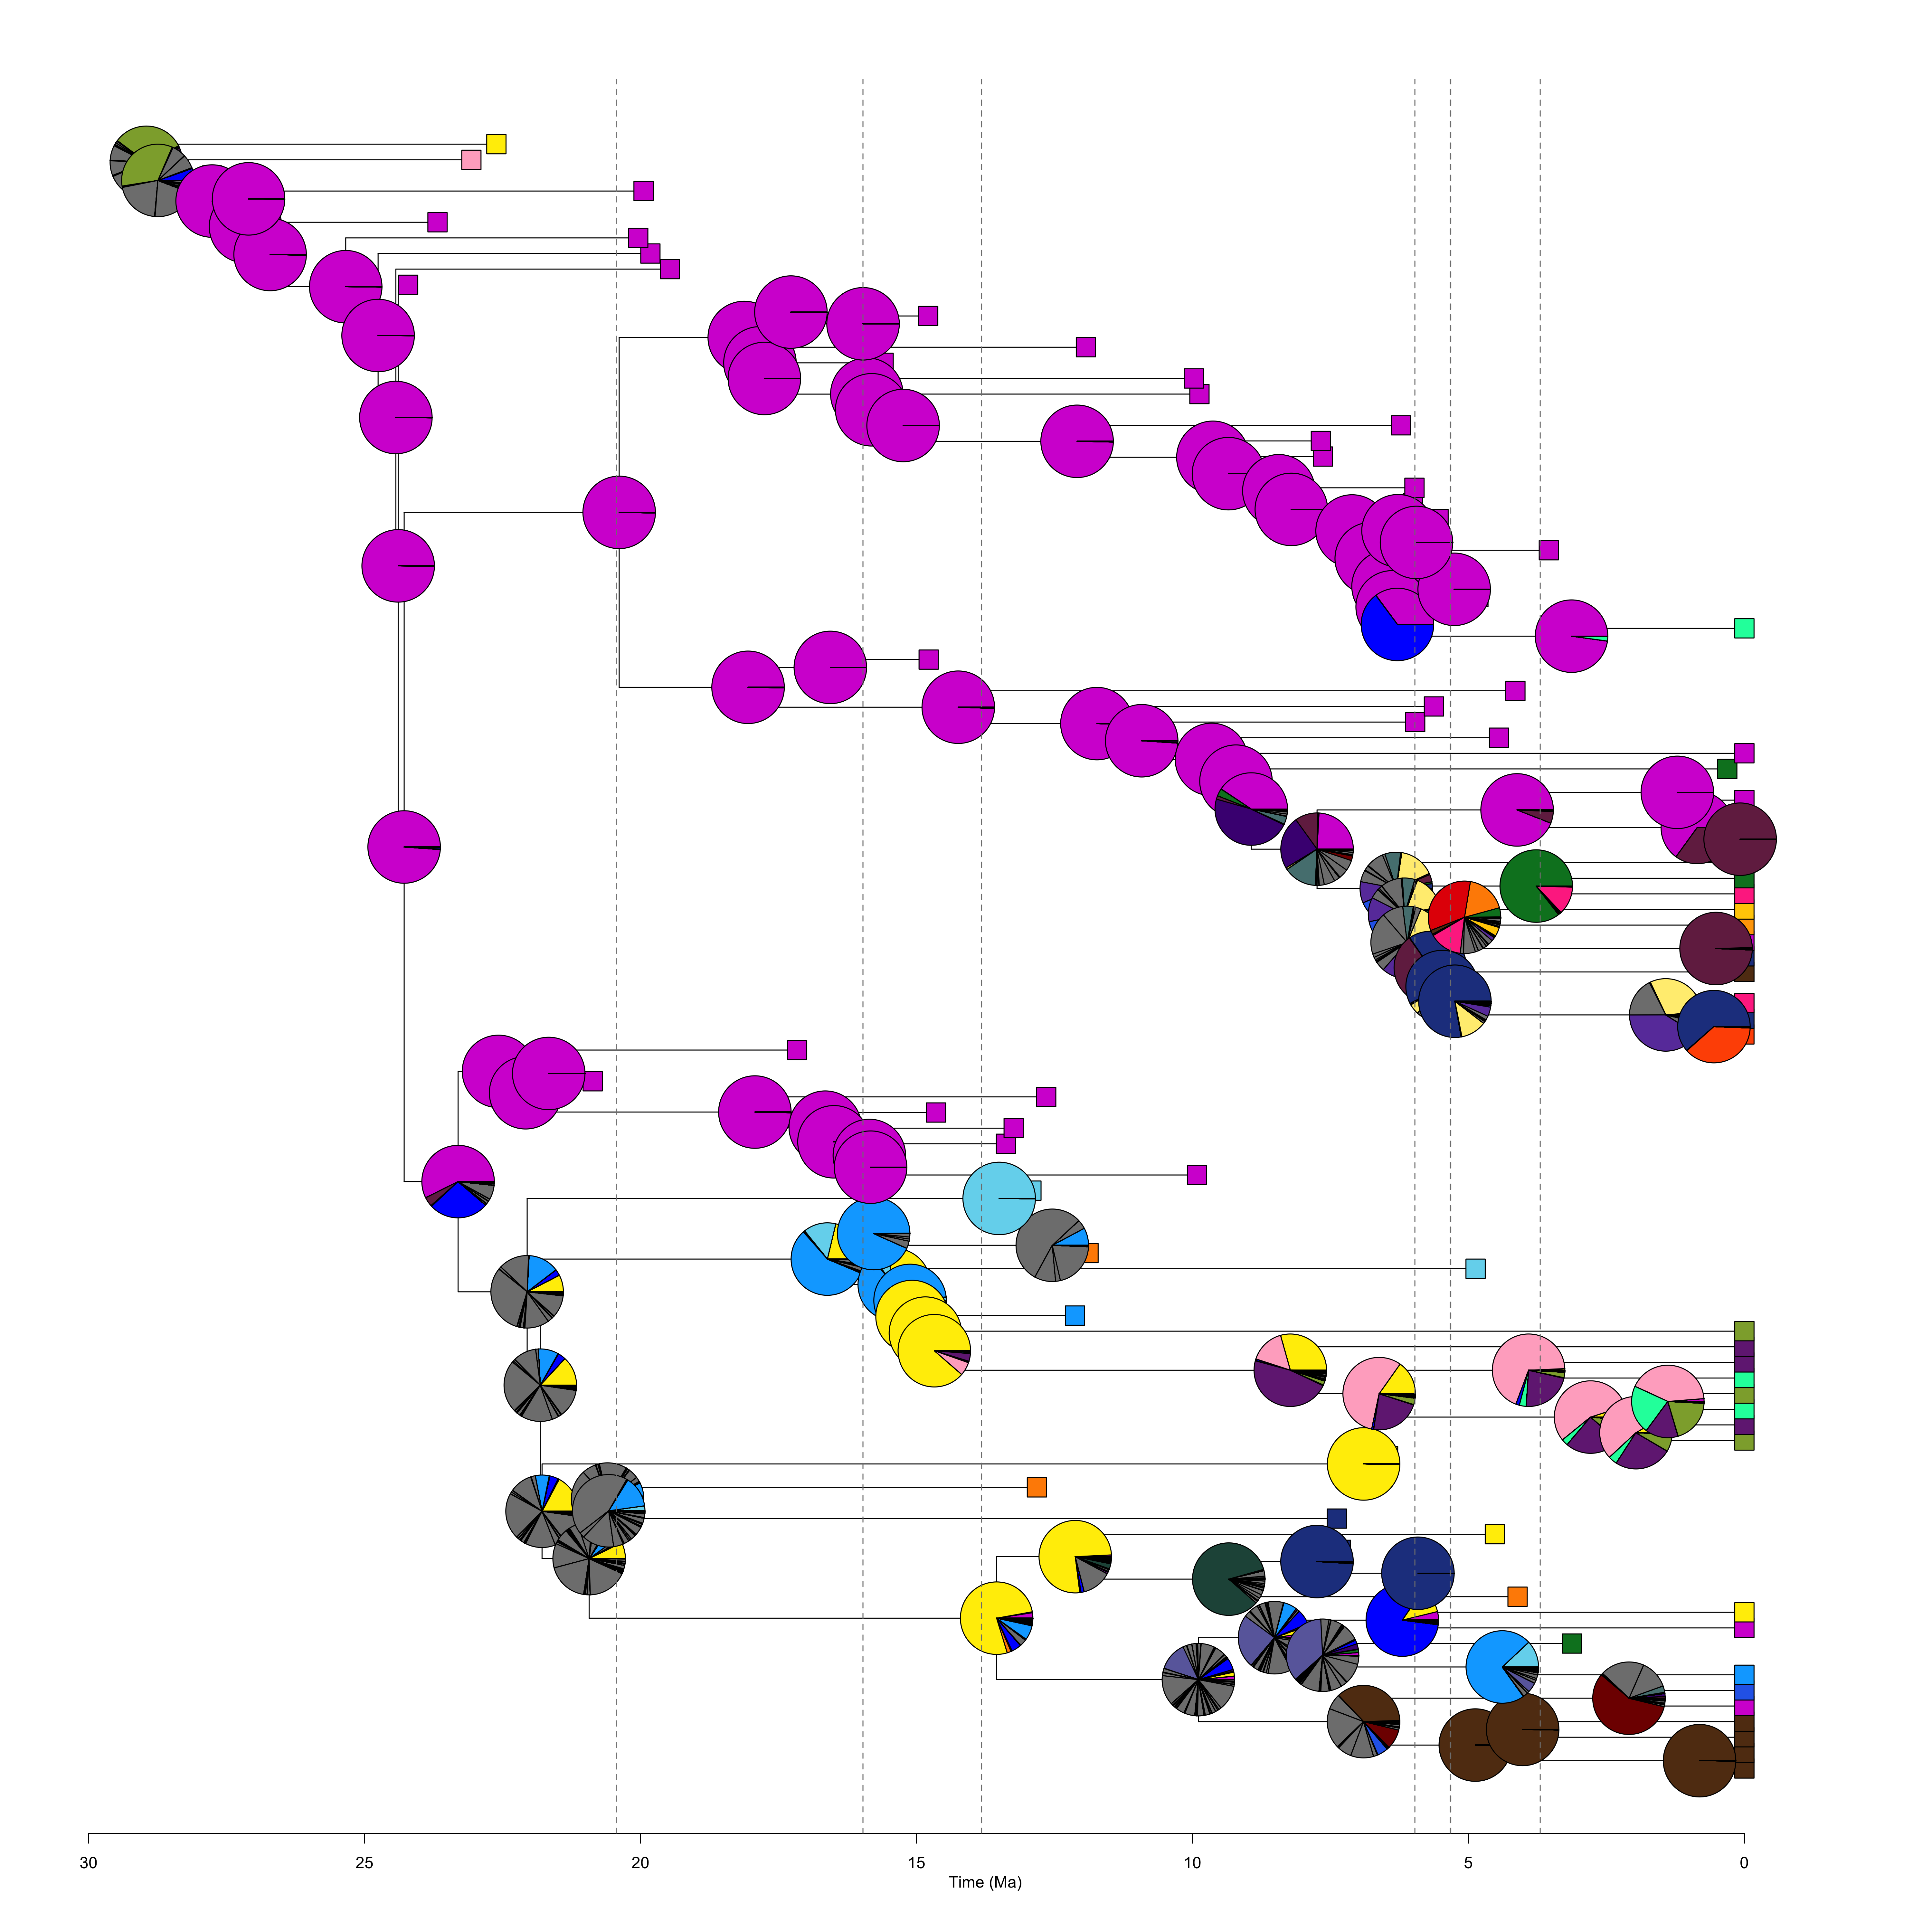
\includegraphics[width = \linewidth]{figures/all-pinnipeds-DEC-unlikely-pies.png}
  \caption{DEC model, impossible and unlikely states removed. Nodes show relative probabilities of each state.}
  \label{fig-all-dec-pie-unlikely}
\end{figure} 

% figure
\begin{figure}[H]
 \centering
  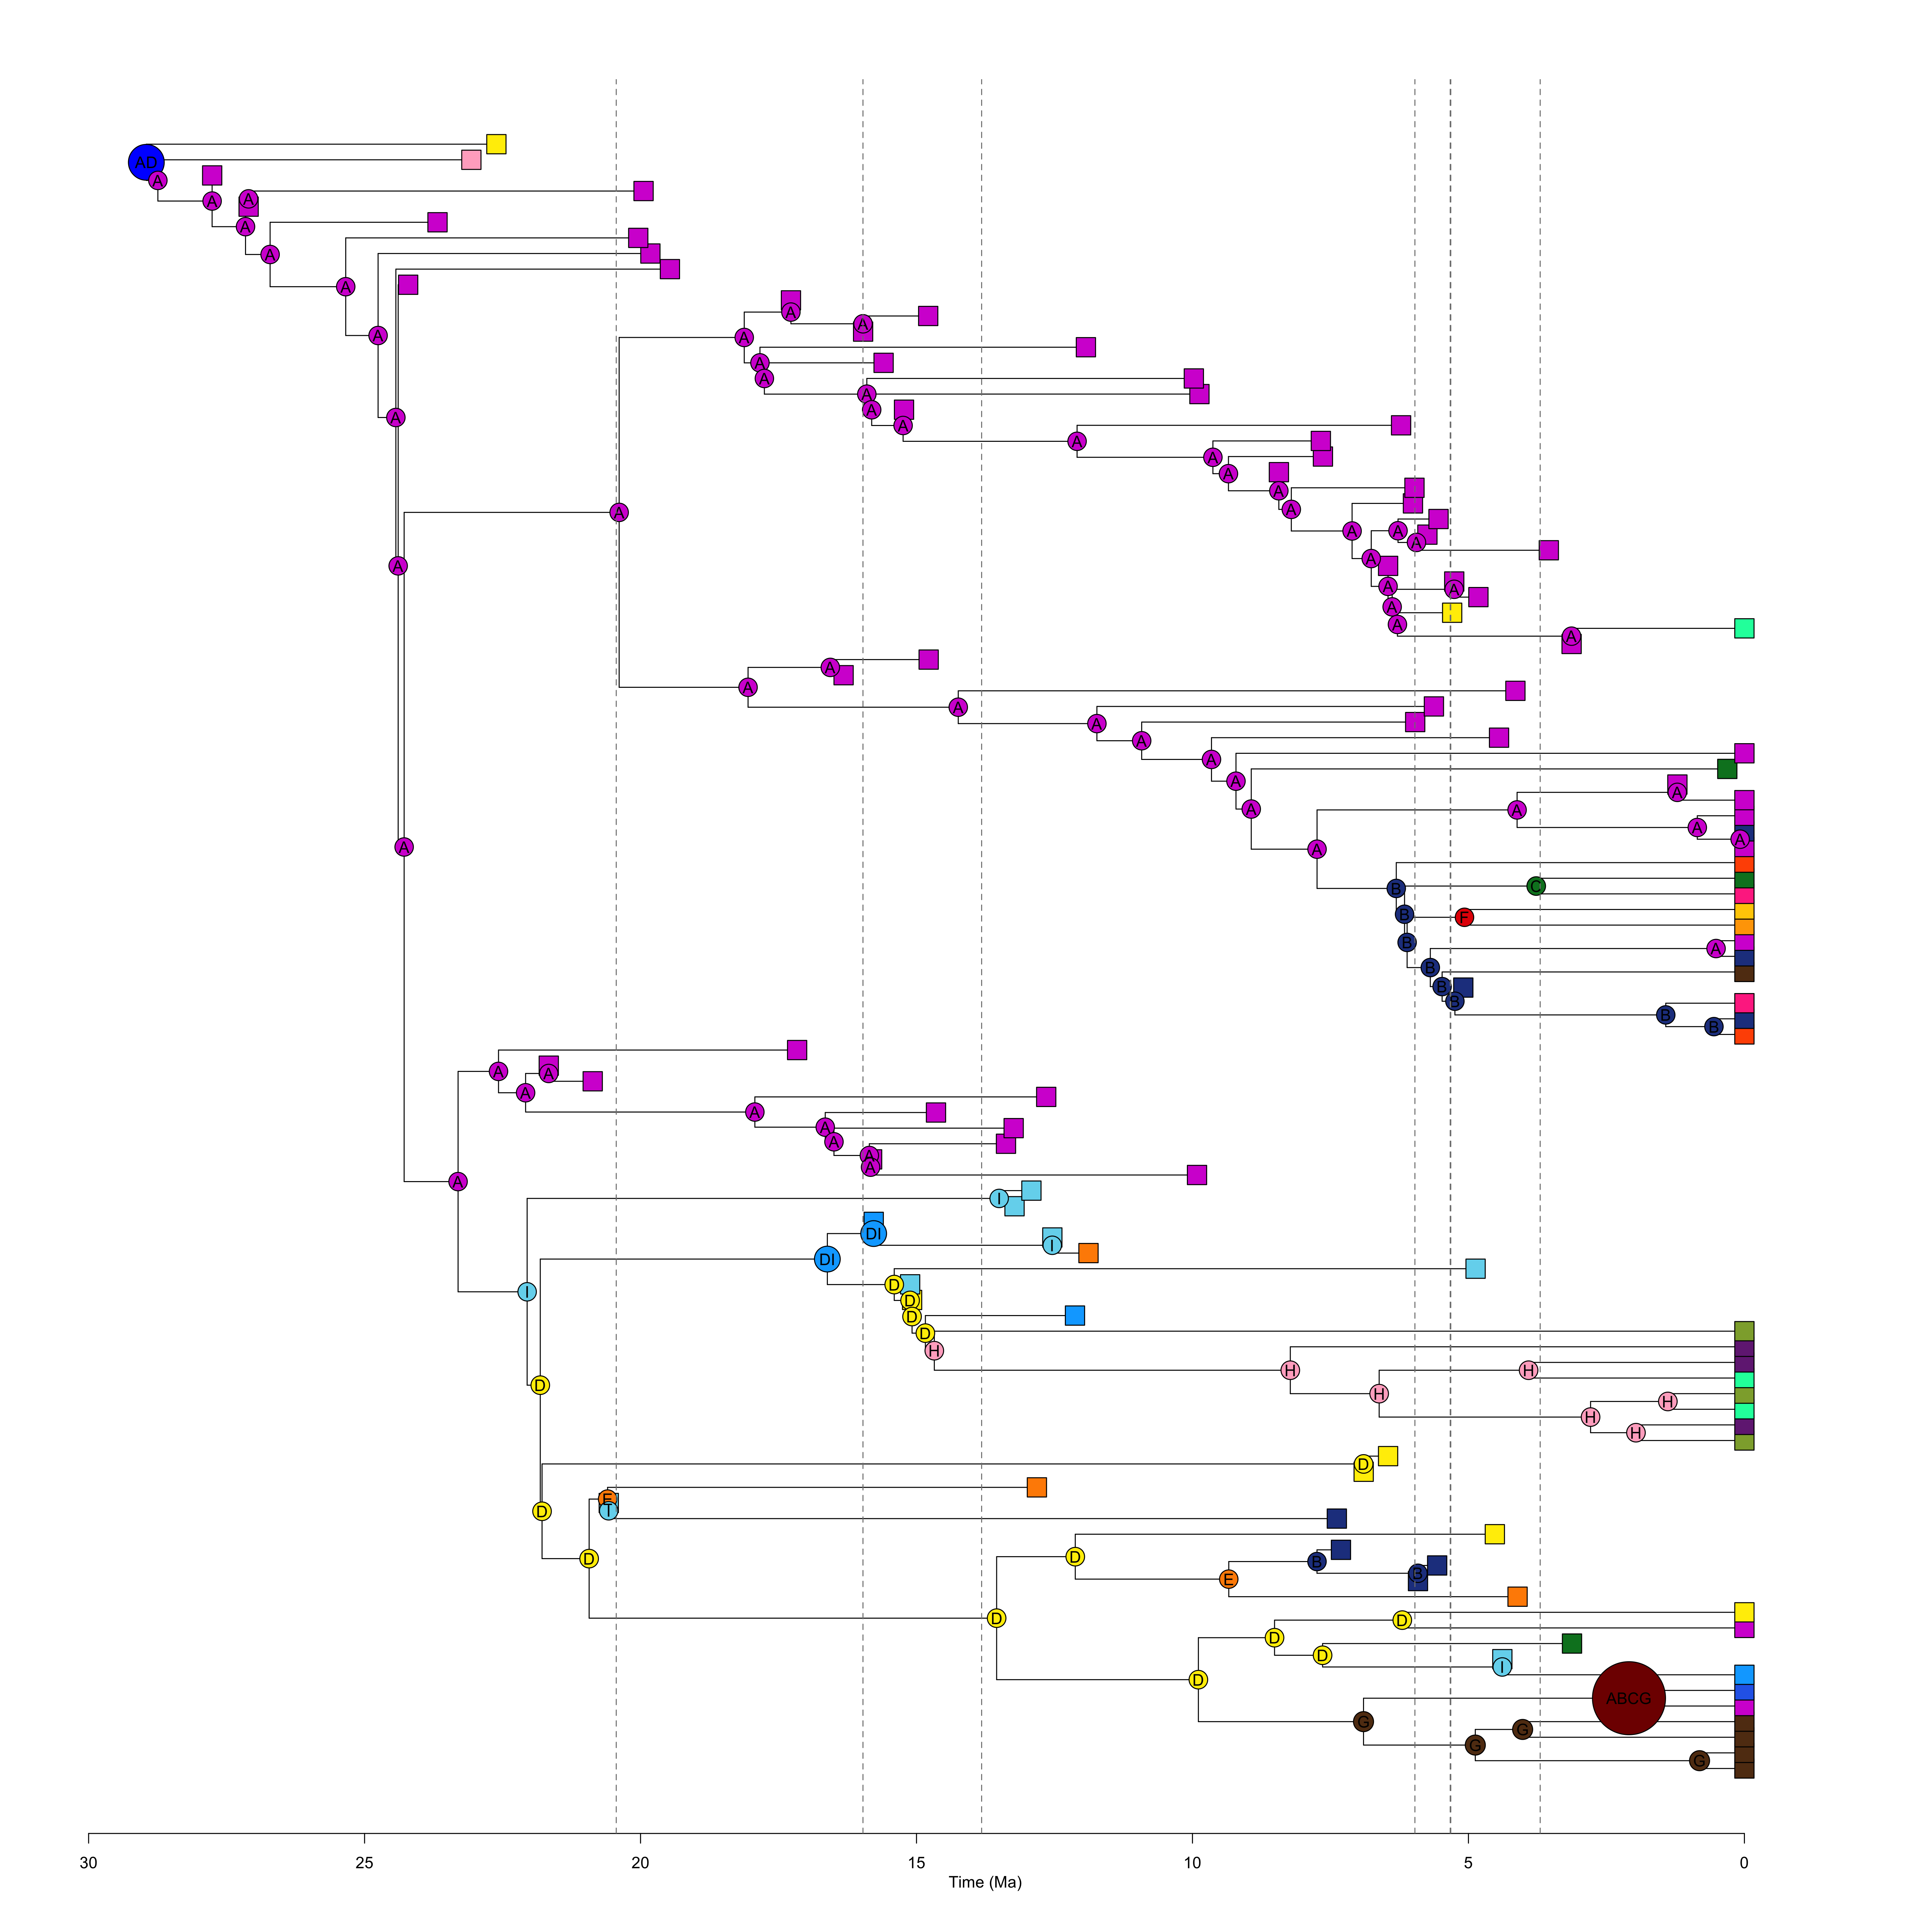
\includegraphics[width = \linewidth]{figures/all-pinnipeds-DECj-unlikely-MLstates.png}
  \caption{DEC+J model, impossible and unlikely states removed. Nodes show Maximum Likelihood states.}
  \label{fig-all-decj-ml-unlikely}
\end{figure} 

% figure
\begin{figure}[H]
 \centering
  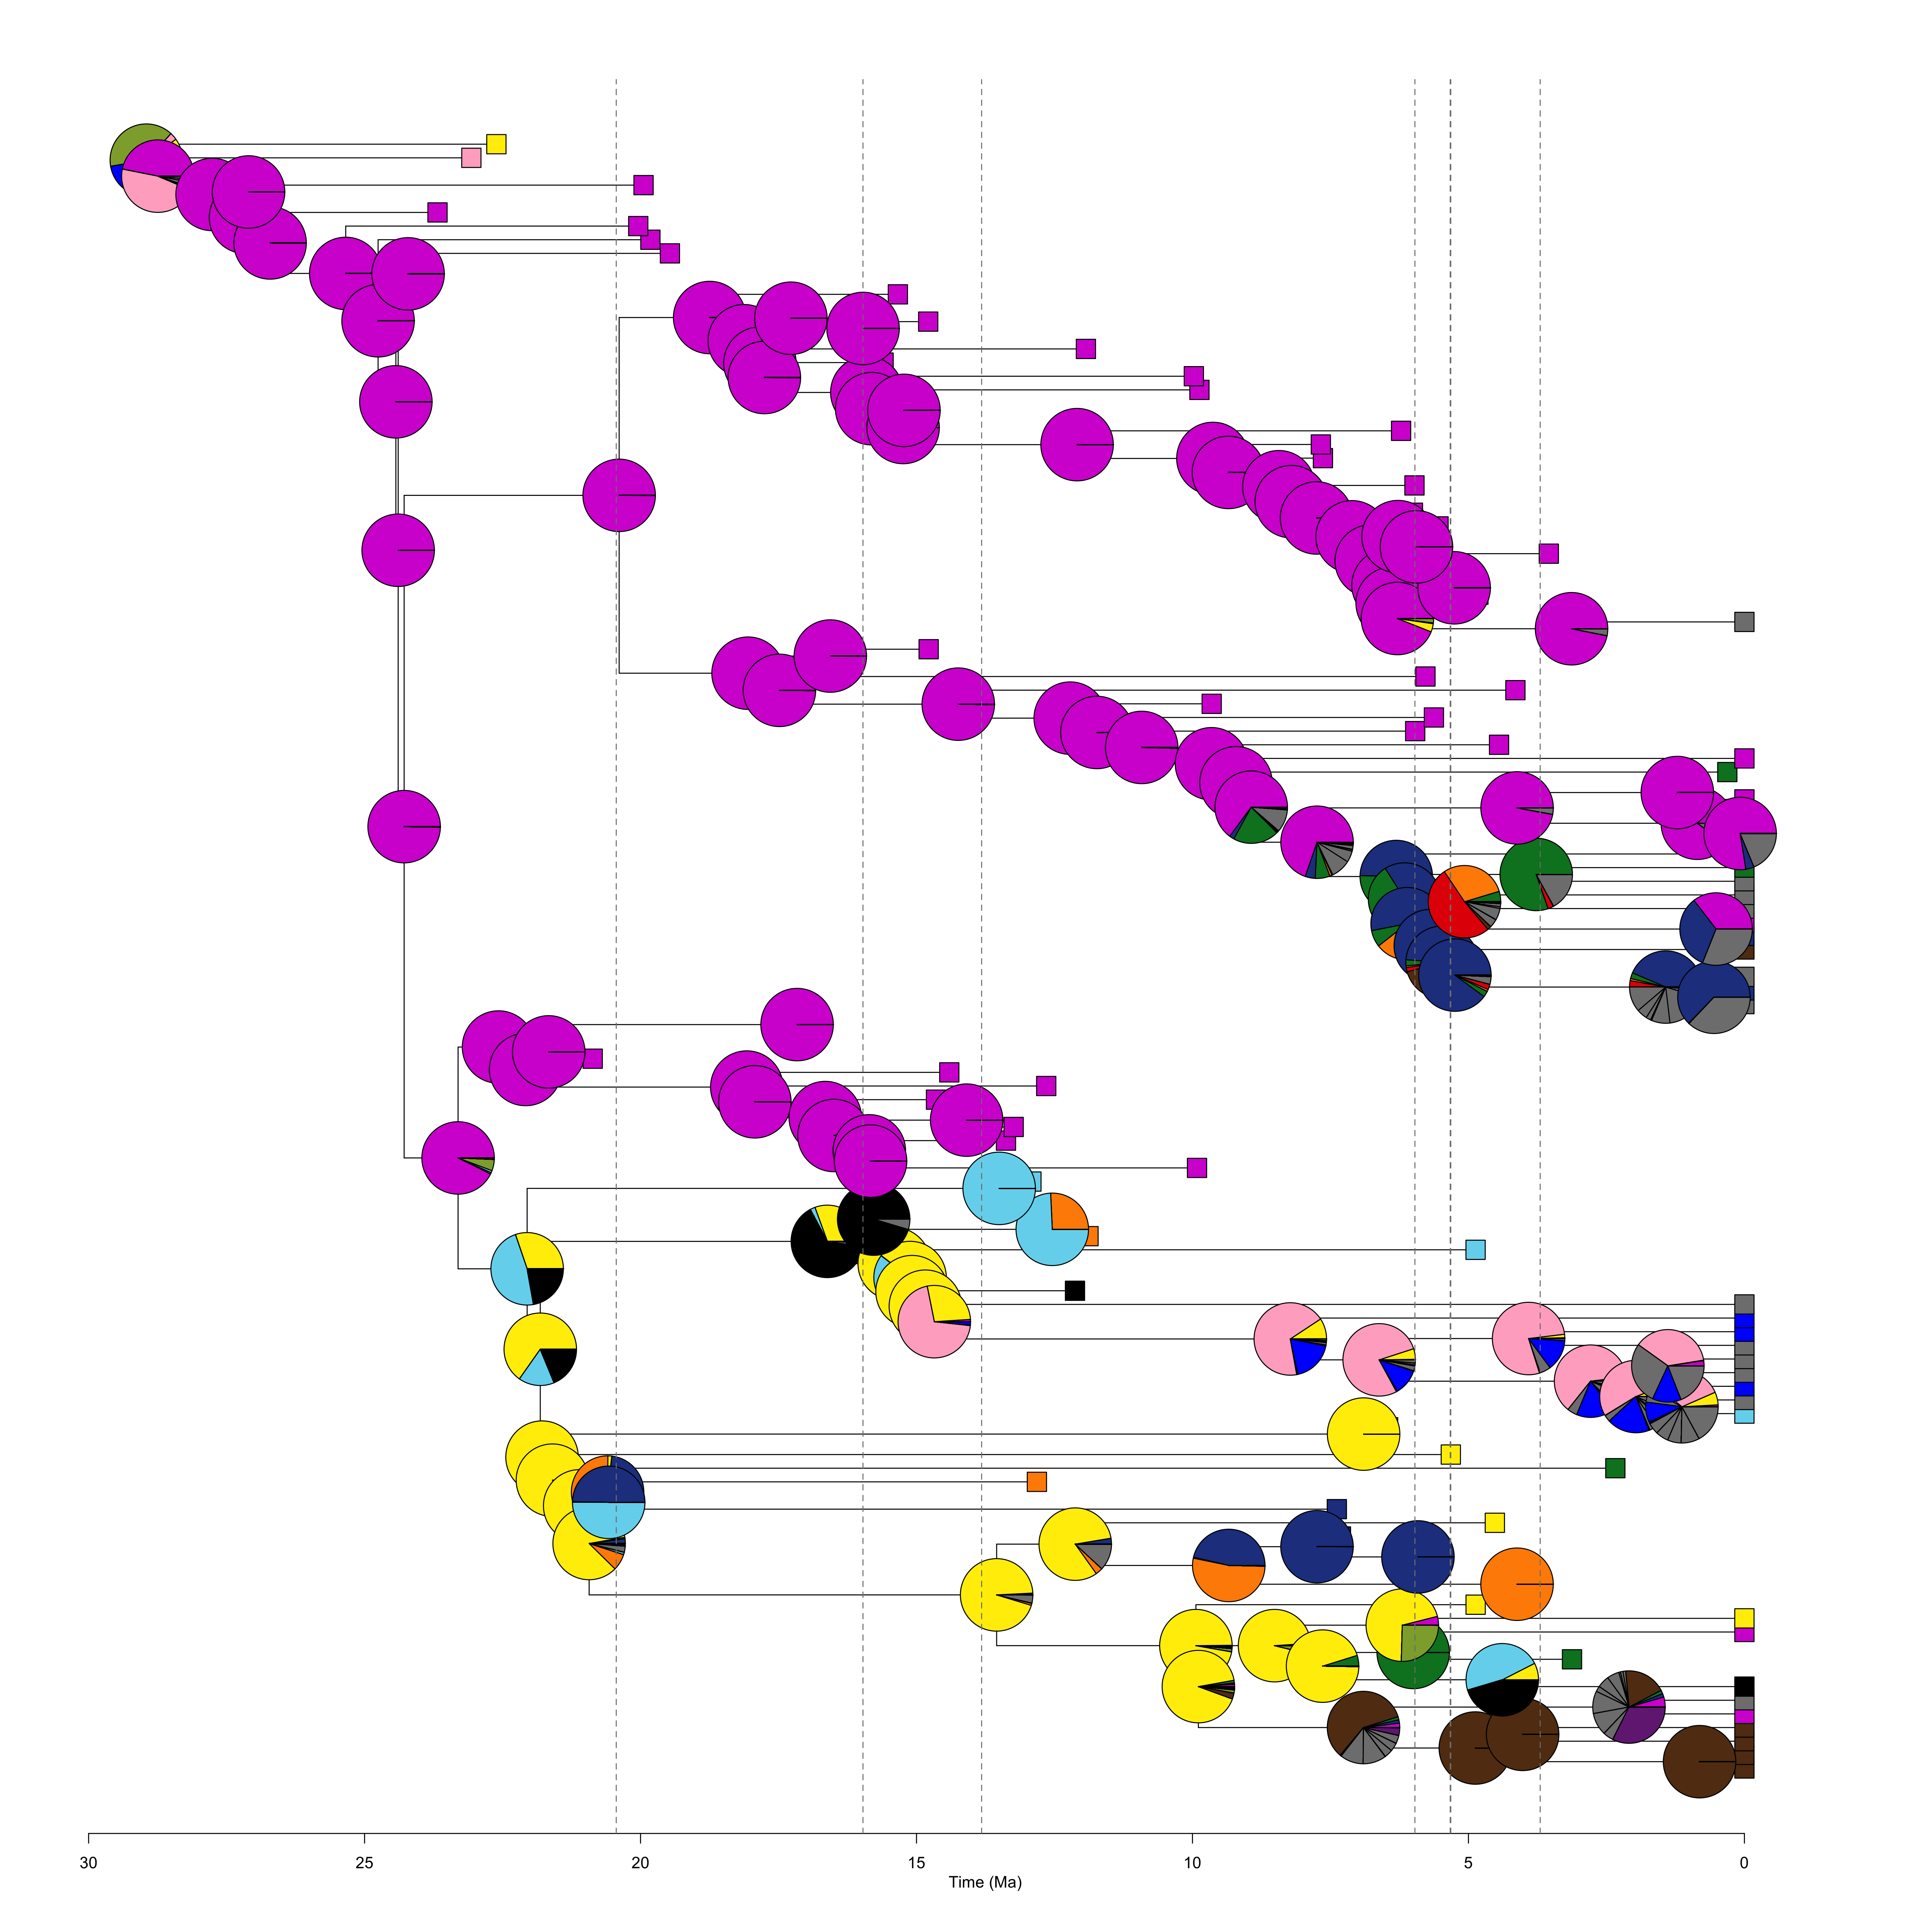
\includegraphics[width = \linewidth]{figures/all-pinnipeds-DECj-unlikely-pies.png}
  \caption{DEC+J model, impossible and unlikely states removed. Nodes show relative probabilities of each state.}
  \label{fig-all-decj-pie-unlikely}
\end{figure} 


%-------------------------------------------------------------------------------
\newpage
\section{The effects of adding fossils}

To understand the influence of fossil taxa on our results, we compared our results with and without fossil taxa included. The results of these analyses are described below. In summary, these results contribute evidence for the key importance of including fossils in these kinds of analyses. Without fossils our results are at best incomplete, as demonstrated by our diversification analyses, and at worst misleading, for example in our biogeography analyses where we were unable to resolve the origins of several major pinniped clades unless fossil taxa were included.

%-------------------------------------------------------------------------------
% Diversification
%-----------------------------------------------------------------------------------
\subsection{Diversification dynamics - extant or fossil taxa only}

\subsubsection{Extant taxa only}

When using the tree containing only extant species, we were unable to detect any of the shifts that we found for the complete tree (Figure \ref{fig-extant-only}), instead diversification rates are constant. There is also very little variation in all rates through time.

% figure
\begin{figure}[H]
  \centering
  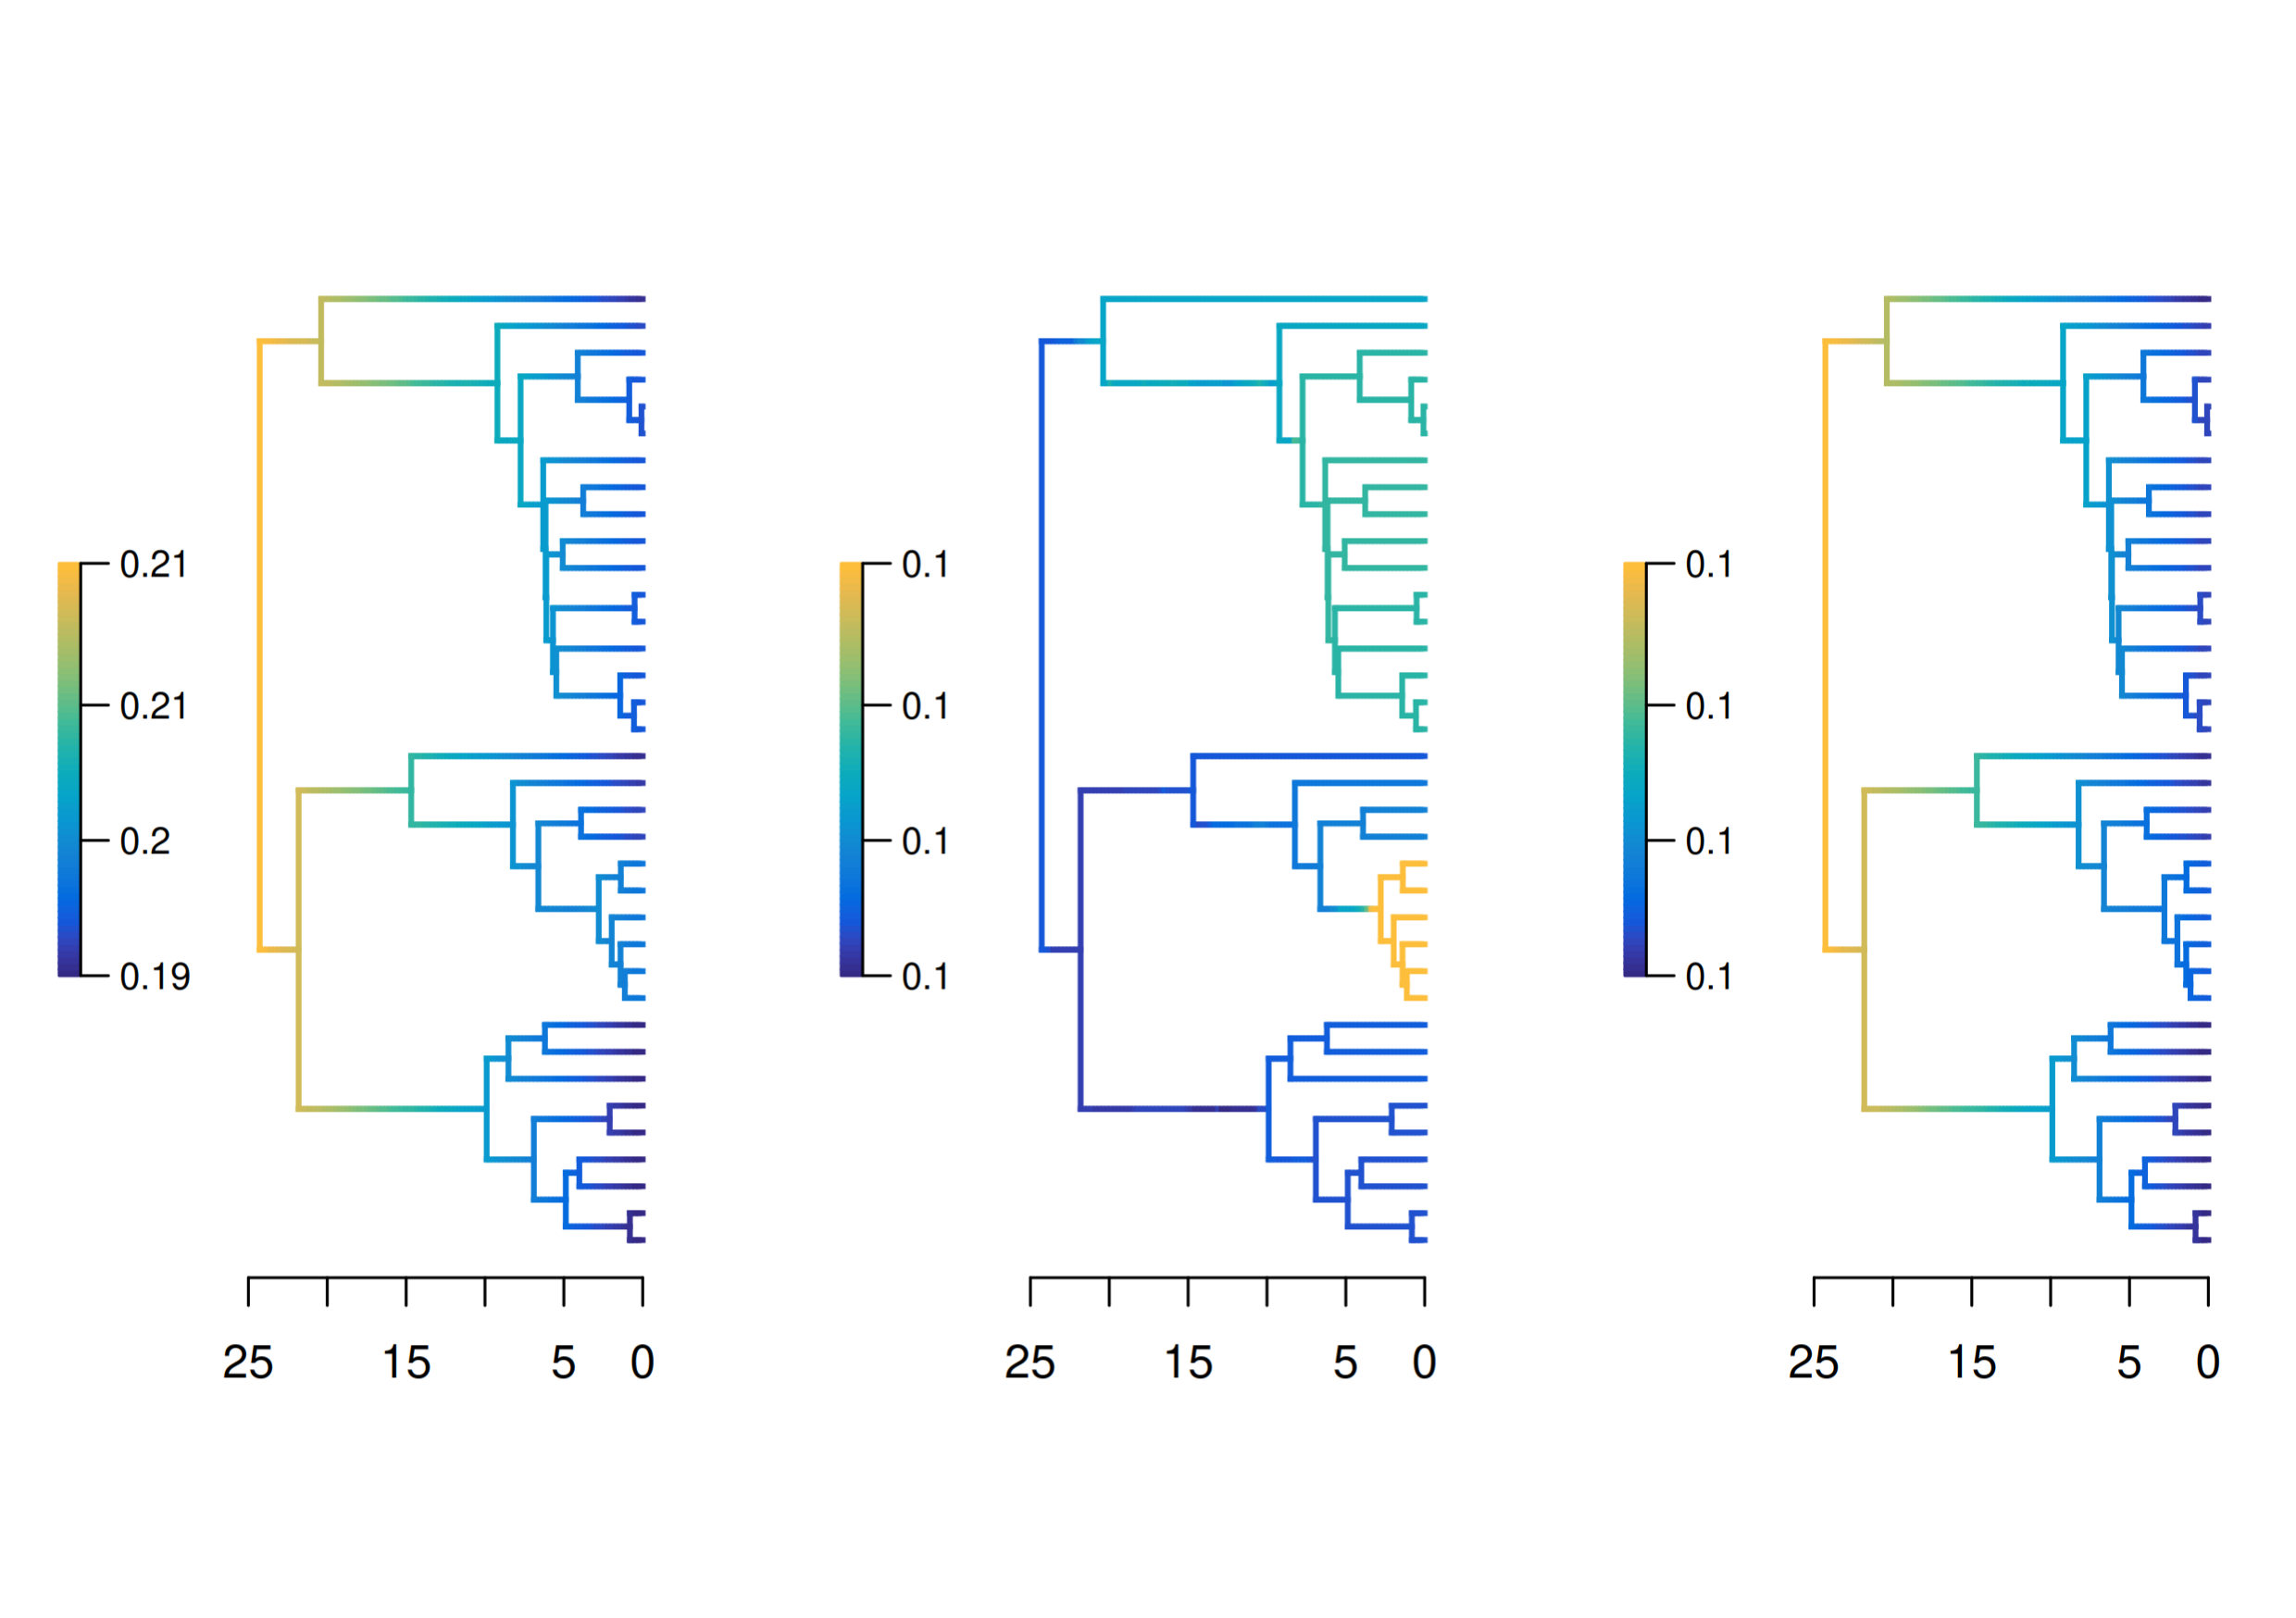
\includegraphics[width = \linewidth]{figures/diversification/extant-only/sensitivity-analysis-extant-only.png}
  \caption{Extant pinnipeds only. $\lambda_{prior} = 1$. Left, middle and right panels indicate speciation, extinction and net diversification rates, respectively. Taxon names have been removed  for readability.}
  \label{fig-extant-only}
\end{figure}

\subsubsection{Fossil taxa only}

Regardless of whether we exclude (Figure \ref{fig-fossil-only-noanc}) or include sampled ancestors (Figure \ref{fig-fossil-only-full}), we still infer a shift in diversification rates in the Odobenidae when analysing the fossil taxa only tree, but the three shifts within Phocidae seen when using all taxa are not detected. The odobenid shifts in the two topologies differ in position, with the tree including sampled ancestors (Figure \ref{fig-fossil-only-full}) showing a shift that is slightly deeper in the tree, therefore grouping a few more lineages than the shift in the tree without sampled ancestors (Figure \ref{fig-fossil-only-noanc}).

% figure
\begin{figure}[H]
  \centering
  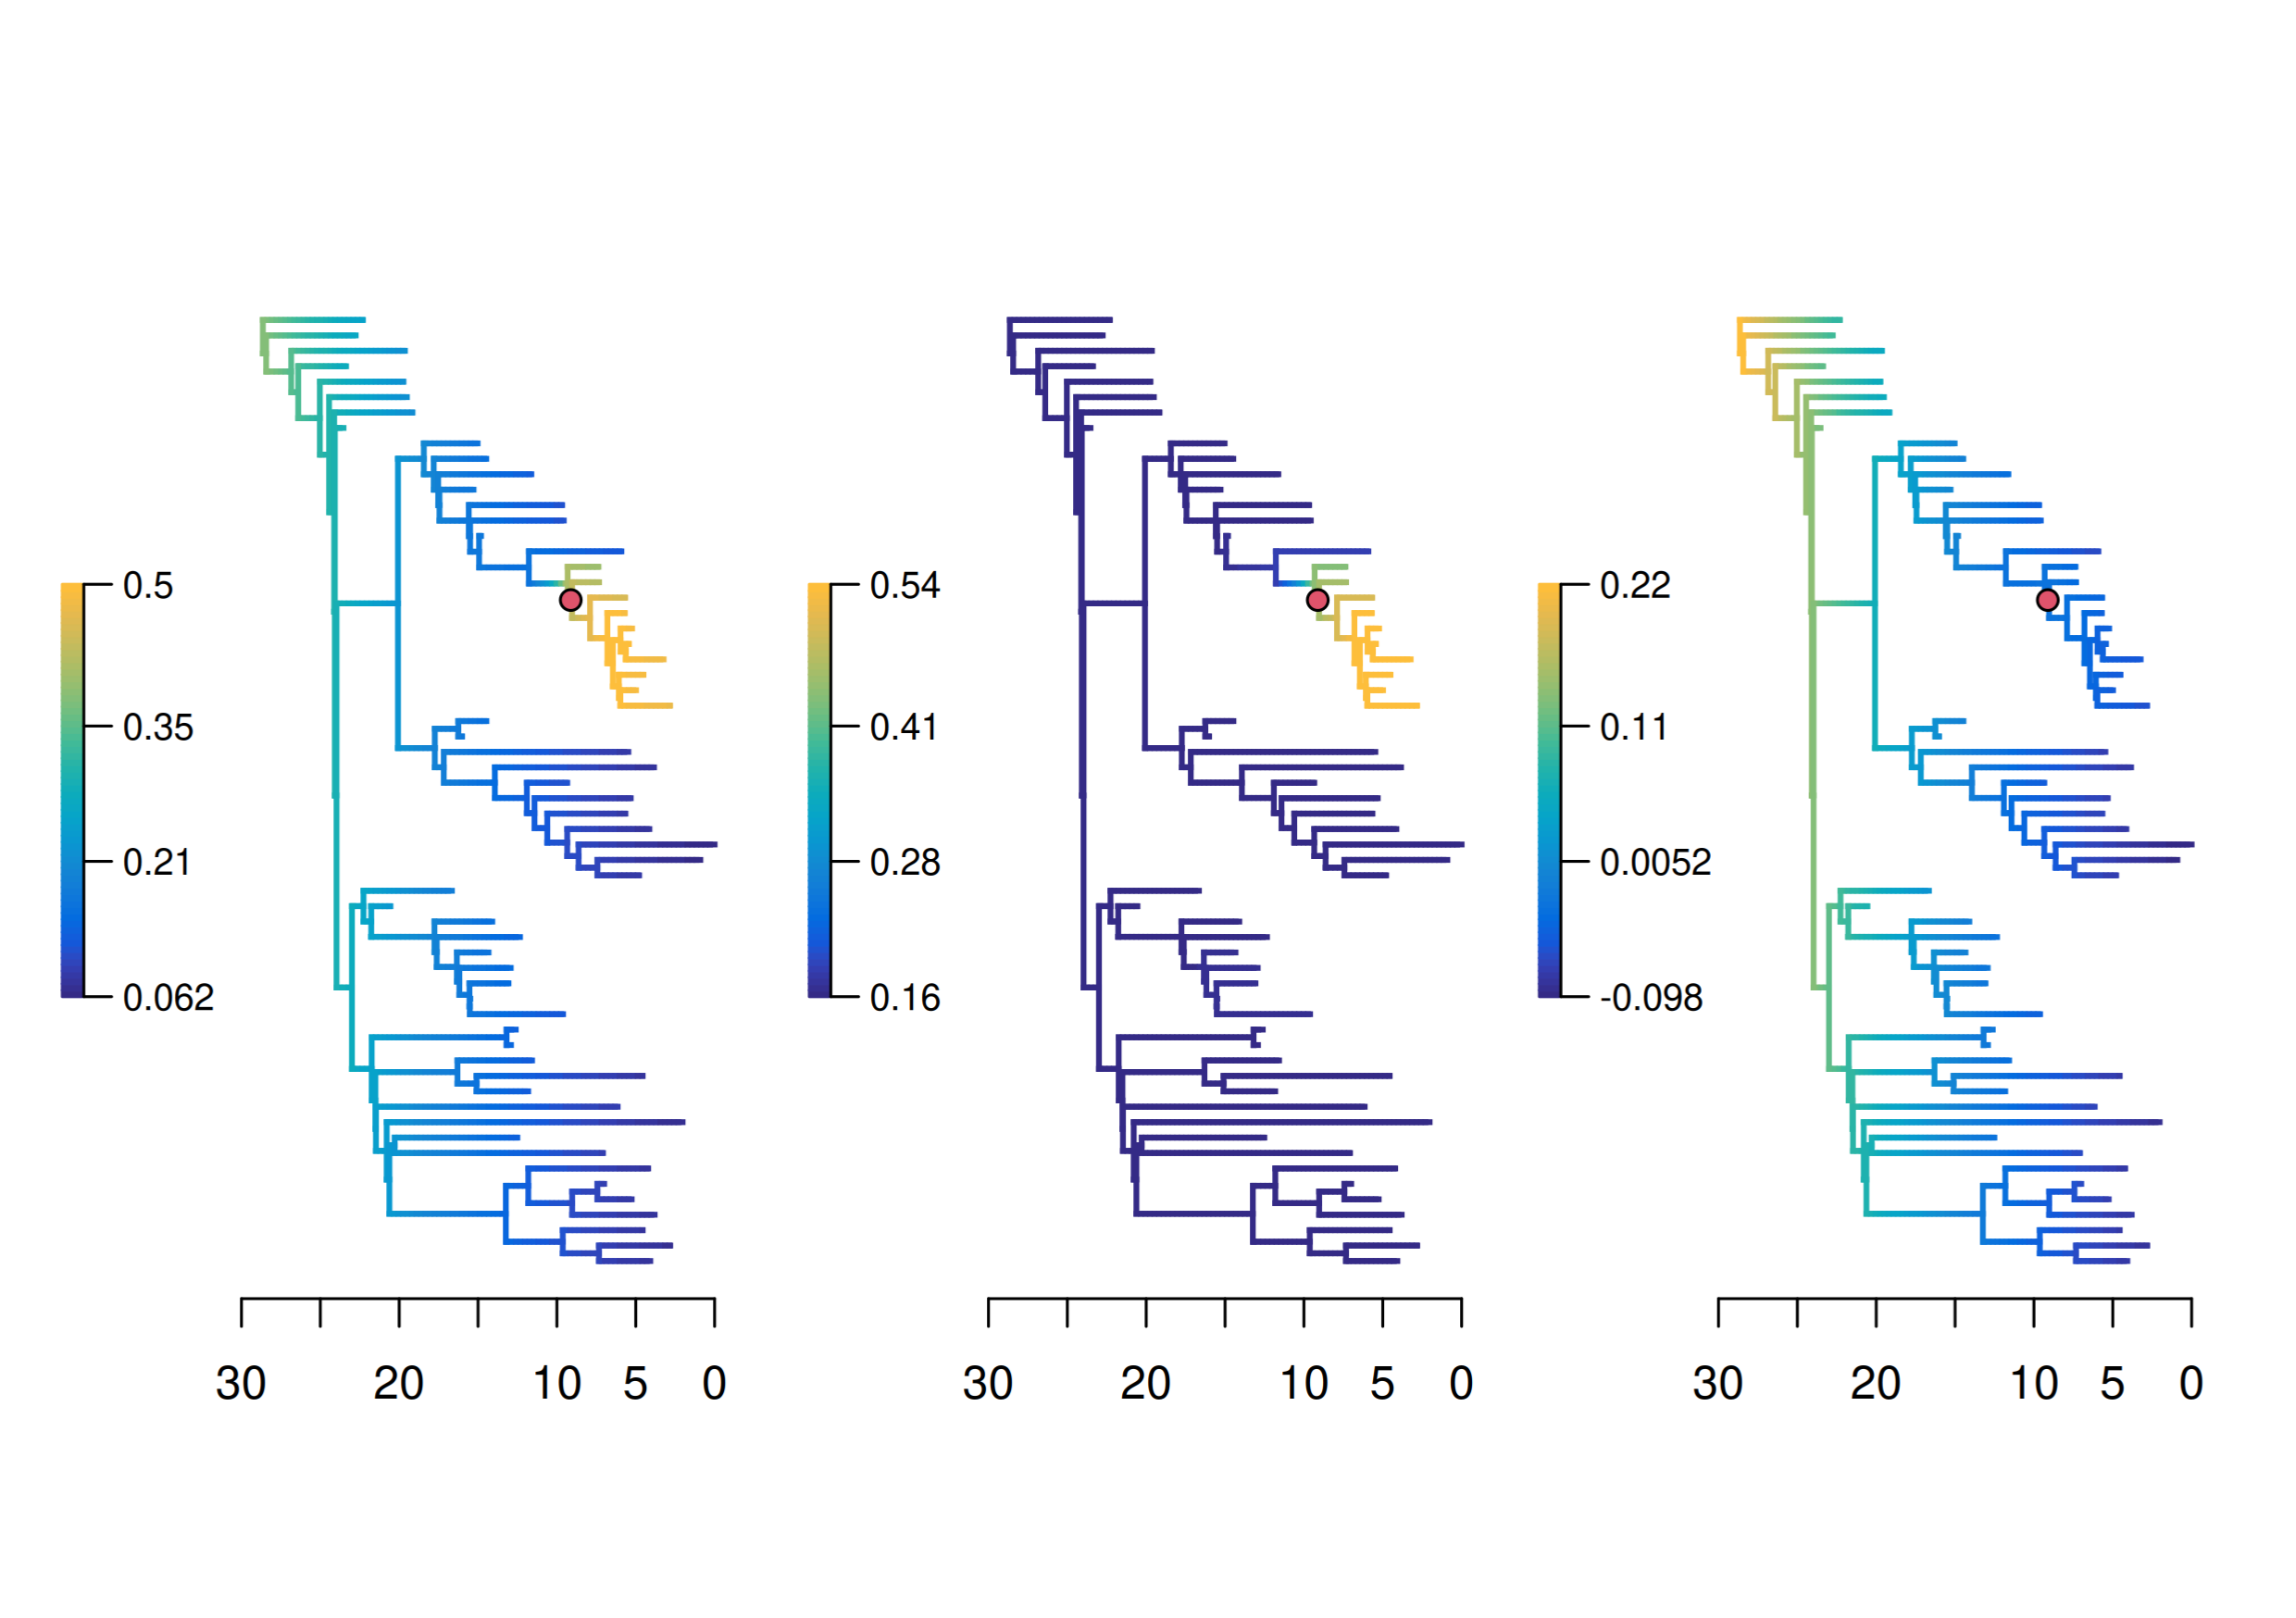
\includegraphics[width = \linewidth]{figures/diversification/fossil-only/sensitivity-analysis-fossil-only.png}
  \caption{Fossil pinnipeds only, excluding sampled ancestors. $\lambda_{prior} = 1$. Left, middle and right panels indicate speciation, extinction and net diversification rates, respectively. Taxon names have been removed  for readability.}
  \label{fig-fossil-only-noanc}
\end{figure}

% figure
\begin{figure}[H]
  \centering
  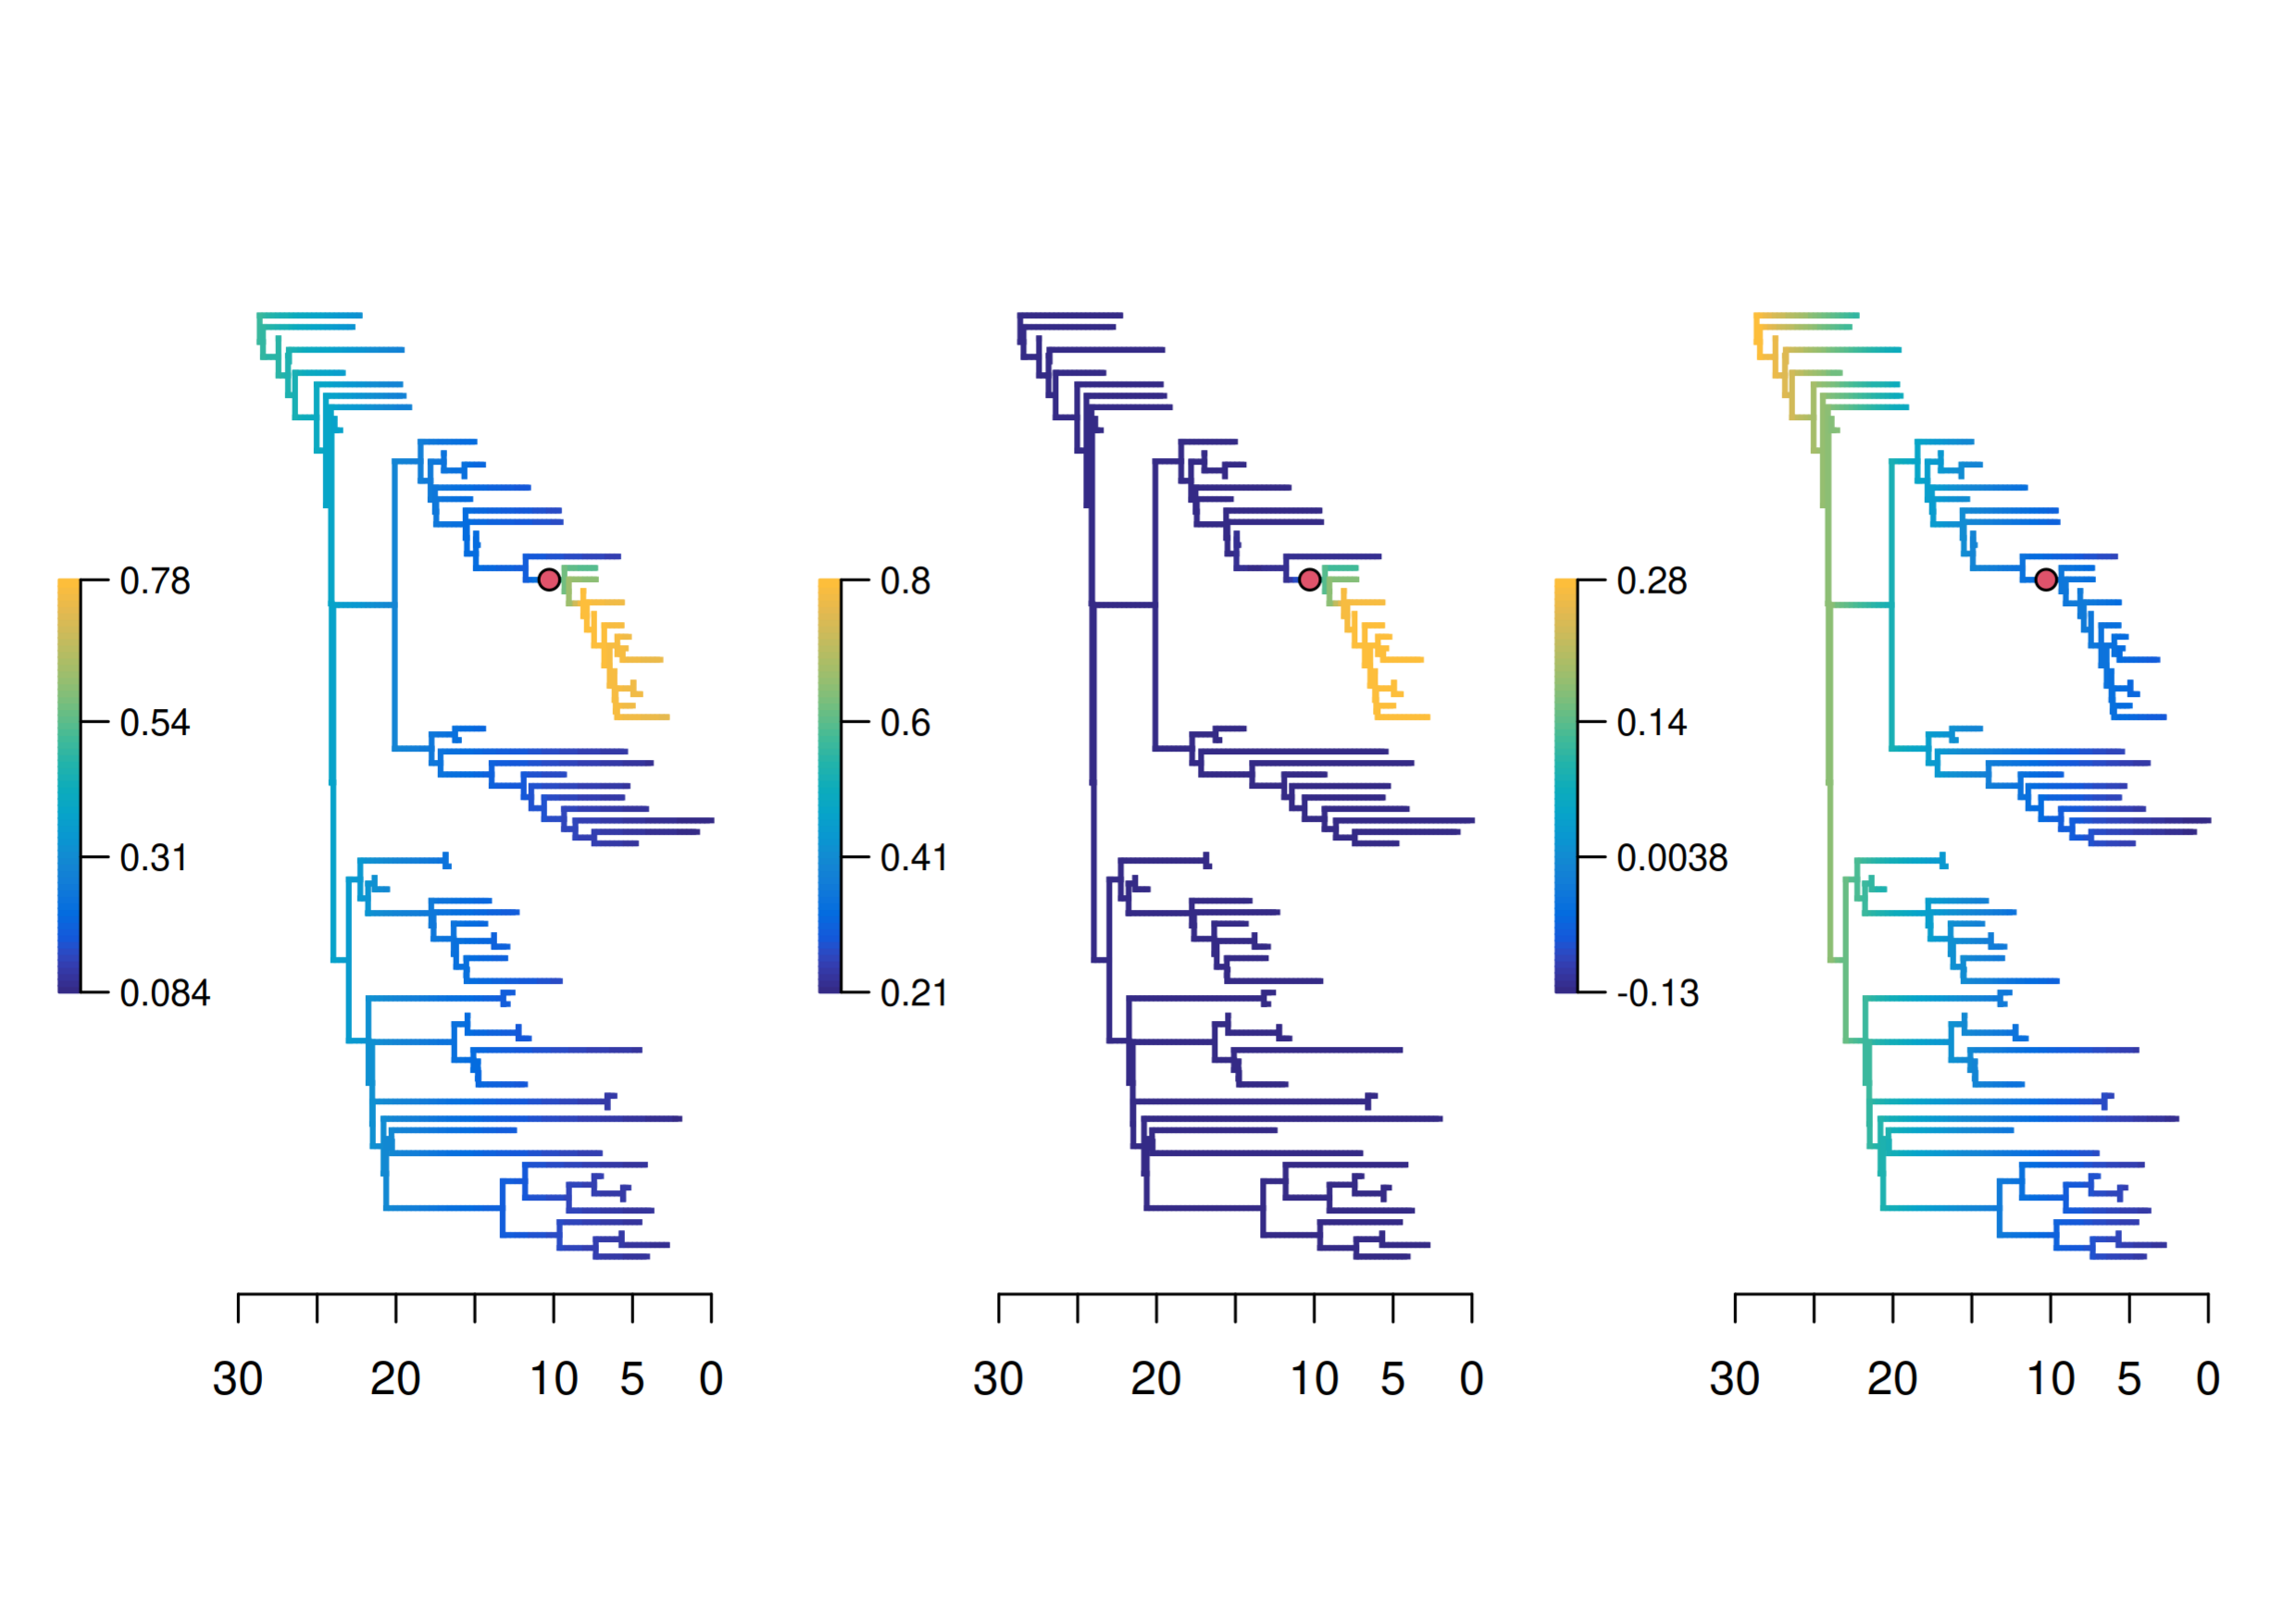
\includegraphics[width = \linewidth]{figures/diversification/fossil-only-with-sampled-ancestors/sensitivity-analysis-fossil-only-full.png}
  \caption{Fossil pinnipeds only, including sampled ancestors. $\lambda_{prior} = 1$. Left, middle and right panels indicate speciation, extinction and net diversification rates, respectively. Taxon names have been removed  for readability.}
  \label{fig-fossil-only-full}
\end{figure}

\subsubsection{The importance of including fossils when inferring diversification dynamics}

Using all taxa (fossil and extant), we infer major shifts in diversification rate in two clades - odobenids and phocids - with the former more dramatically impacting the overall diversification dynamics for the group. Critically, excluding fossil taxa led to an inferred scenario of constant-rate diversification for pinnipeds. This is driven by the fact that extant odobenids are represented by just one taxon, the walrus (\textit{Odobenus rosmarus}), thus extant only analyses exclude the substantial extinct diversity of the clade. Similar results have been seen in cetaceans. Using extant only phylogenies, diversification analyses detect only one significant shift in diversification in delphinids (dolphins; \citealt{rabosky2014automatic}). Conversely, inferring a metatree using the same methodology as ours, Lloyd \& Slater (\citeyear{lloyd2021total}) found an additional shift in ziphiids (beaked whales), leading to important discussions about the role of ecological flexibility and sexual selection in the diversification of Cetacea \citep{lloyd2021total}. Note that in both pinnipeds and cetaceans, the results of extant-only analyses are not wrong \textit{per se}; they detect most shifts that are detected in phylogenies with both fossil and extant taxa. However, they miss interesting patterns and obscure the true history of the groups involved.

%-------------------------------------------------------------
\subsection{Biogeographical history - extant or fossil taxa only}
%-------------------------------------------------------------

Regardless of whether we based our analyses on extant taxa only, fossil taxa only, or all taxa, the DEC+J model received favourable support over the DEC model, based on AICc scores (Table \ref{table-biogeo-results}). Results were similar whether only impossible, or impossible and unlikely states were removed (Table \ref{table-unlikely-fossil}).

% table of full results
% Table of full biogeo results
\begin{longtable}{ccccccc}

\caption{Results of model fits from BioGeoBEARS analysis for all pinnipeds, and for fossil and extant taxa separately. Impossible and unlikely area-combinations were excluded (see text). DEC = dispersal-extinction-cladogenesis; DEC + J = DEC model with jump dispersal; lnL = log-likelihood values; AICc = sample-size corrected Akaike information criterion; d = dispersal rate (range expansion) along each branch within the phylogeny; e = extinction rate (range contraction) along each branch within the phylogeny; j, relative weight of jump dispersal in each model.
}\\

\hline
\textbf{Taxa} & 
\textbf{Model} & 
\textbf{lnL} &
\textbf{AICc} &
\textbf{d}&
\textbf{e} &
\textbf{j}\\
\hline
All &
DEC &
-274.9 &
553.7 &
0.0110 &
0.0208 &
-\\

 &
DEC+J &
-258.4 &
522.7 &
0.0068 &
0.0040 &
0.0159 \\

Fossil &
DEC &
-139.3 &
282.7 &
0.0100 &
0.0100 &
-\\

 &
DEC+J &
-119.1 &
244.3 &
0.0018 &
0.0083 &
0.0128 \\

Extant &
DEC &
-134.0 &
272.1 &
0.0141 &
0.0011 &
-\\

 &
DEC+J &
-129.5 &
265.0 &
0.0117 &
0.0000 &
0.0319\\

\hline

\label{table-biogeo-results}
\end{longtable}

% table of unlikely results
% Table of unlikely results
\begin{longtable}{ccccccc}

\caption{Results of model fits from BioGeoBEARS analysis for fossil and extant taxa separately. Impossible and unlikely area-combinations were excluded (see text). DEC = dispersal-extinction-cladogenesis; DEC + J = DEC model with jump dispersal; lnL = log-likelihood values; AICc = sample-size corrected Akaike information criterion; d = dispersal rate (range expansion) along each branch within the phylogeny; e = extinction rate (range contraction) along each branch within the phylogeny; j, relative weight of jump dispersal in each model.
}\\

\hline
\textbf{Taxa} & 
\textbf{Model} &
\textbf{lnL} &
\textbf{AICc} &
\textbf{d}&
\textbf{e} &
\textbf{j}\\
\hline
Fossil &
DEC &
-145.2 &
294.4 &
0.0127 &
0.0353 &
-\\

 &
DEC+J &
-117.7 &
241.4 &
0.0034 &
0.0068 &
0.0133 \\

Extant &
DEC &
-125.4 &
254.9 &
0.0217 &
0.0000 &
-\\

 &
DEC+J &
-121.5 &
248.9 &
0.0187 &
0.0000 &
0.0307\\
\hline

\label{table-unlikely-fossil}
\end{longtable}

% figure
\begin{figure}[H]
 \centering
  \includegraphics[width = \linewidth]{figures/biogeography-insets-all.png}
  \caption{Biogeographic state estimations for the major groups within our study. Pies show the relative proportions of different states at that node. See Figure \ref{fig-legend} for legend. States with proportions less than 0.1 are shown in gray. A) All taxa, DEC; B) all taxa, DEC+J (also in main text results); C) fossil taxa, DEC; D) fossil taxa, DEC+J; E) extant taxa, DEC; F) extant taxa, DEC+J.}
  \label{fig-nodes-all}
\end{figure} 

\subsubsection{Extant taxa only}
In contrast to the well-supported results from the complete tree, ancestral range inference for the common ancestor of crown pinnipeds is highly ambiguous (Figures \ref{fig-nodes-all}, \ref{fig-extant-dec-ml}-\ref{fig-extant-decj-pie}). Under the preferred DEC+J model, the most likely ancestral range was North Pacific + North Atlantic, but with marginal probability P = 0.09, and comparably supported models add additional areas to the ancestral range. The most likely ancestral range under DEC is North Pacific + North Atlantic + Arctic, but again support is low (P = 0.06) and other area combinations receive comparable support. Similarly, we obtained ambiguous results for crown Phocidae. As for the complete tree, North Atlantic is the most likely area of ancestry but support in these analyses is low (DEC: P = 0.16, DEC+J: P = 0.10). Support for a North Pacific origin of Otarioidea (Odobenidae plus Otariidae) is stronger than support for the phocid node, but still lower than in simultaneous analysis of extant and extinct taxa (DEC: P = 0.60, DEC+J: P = 0.82).

% figure
\begin{figure}[H]
 \centering
  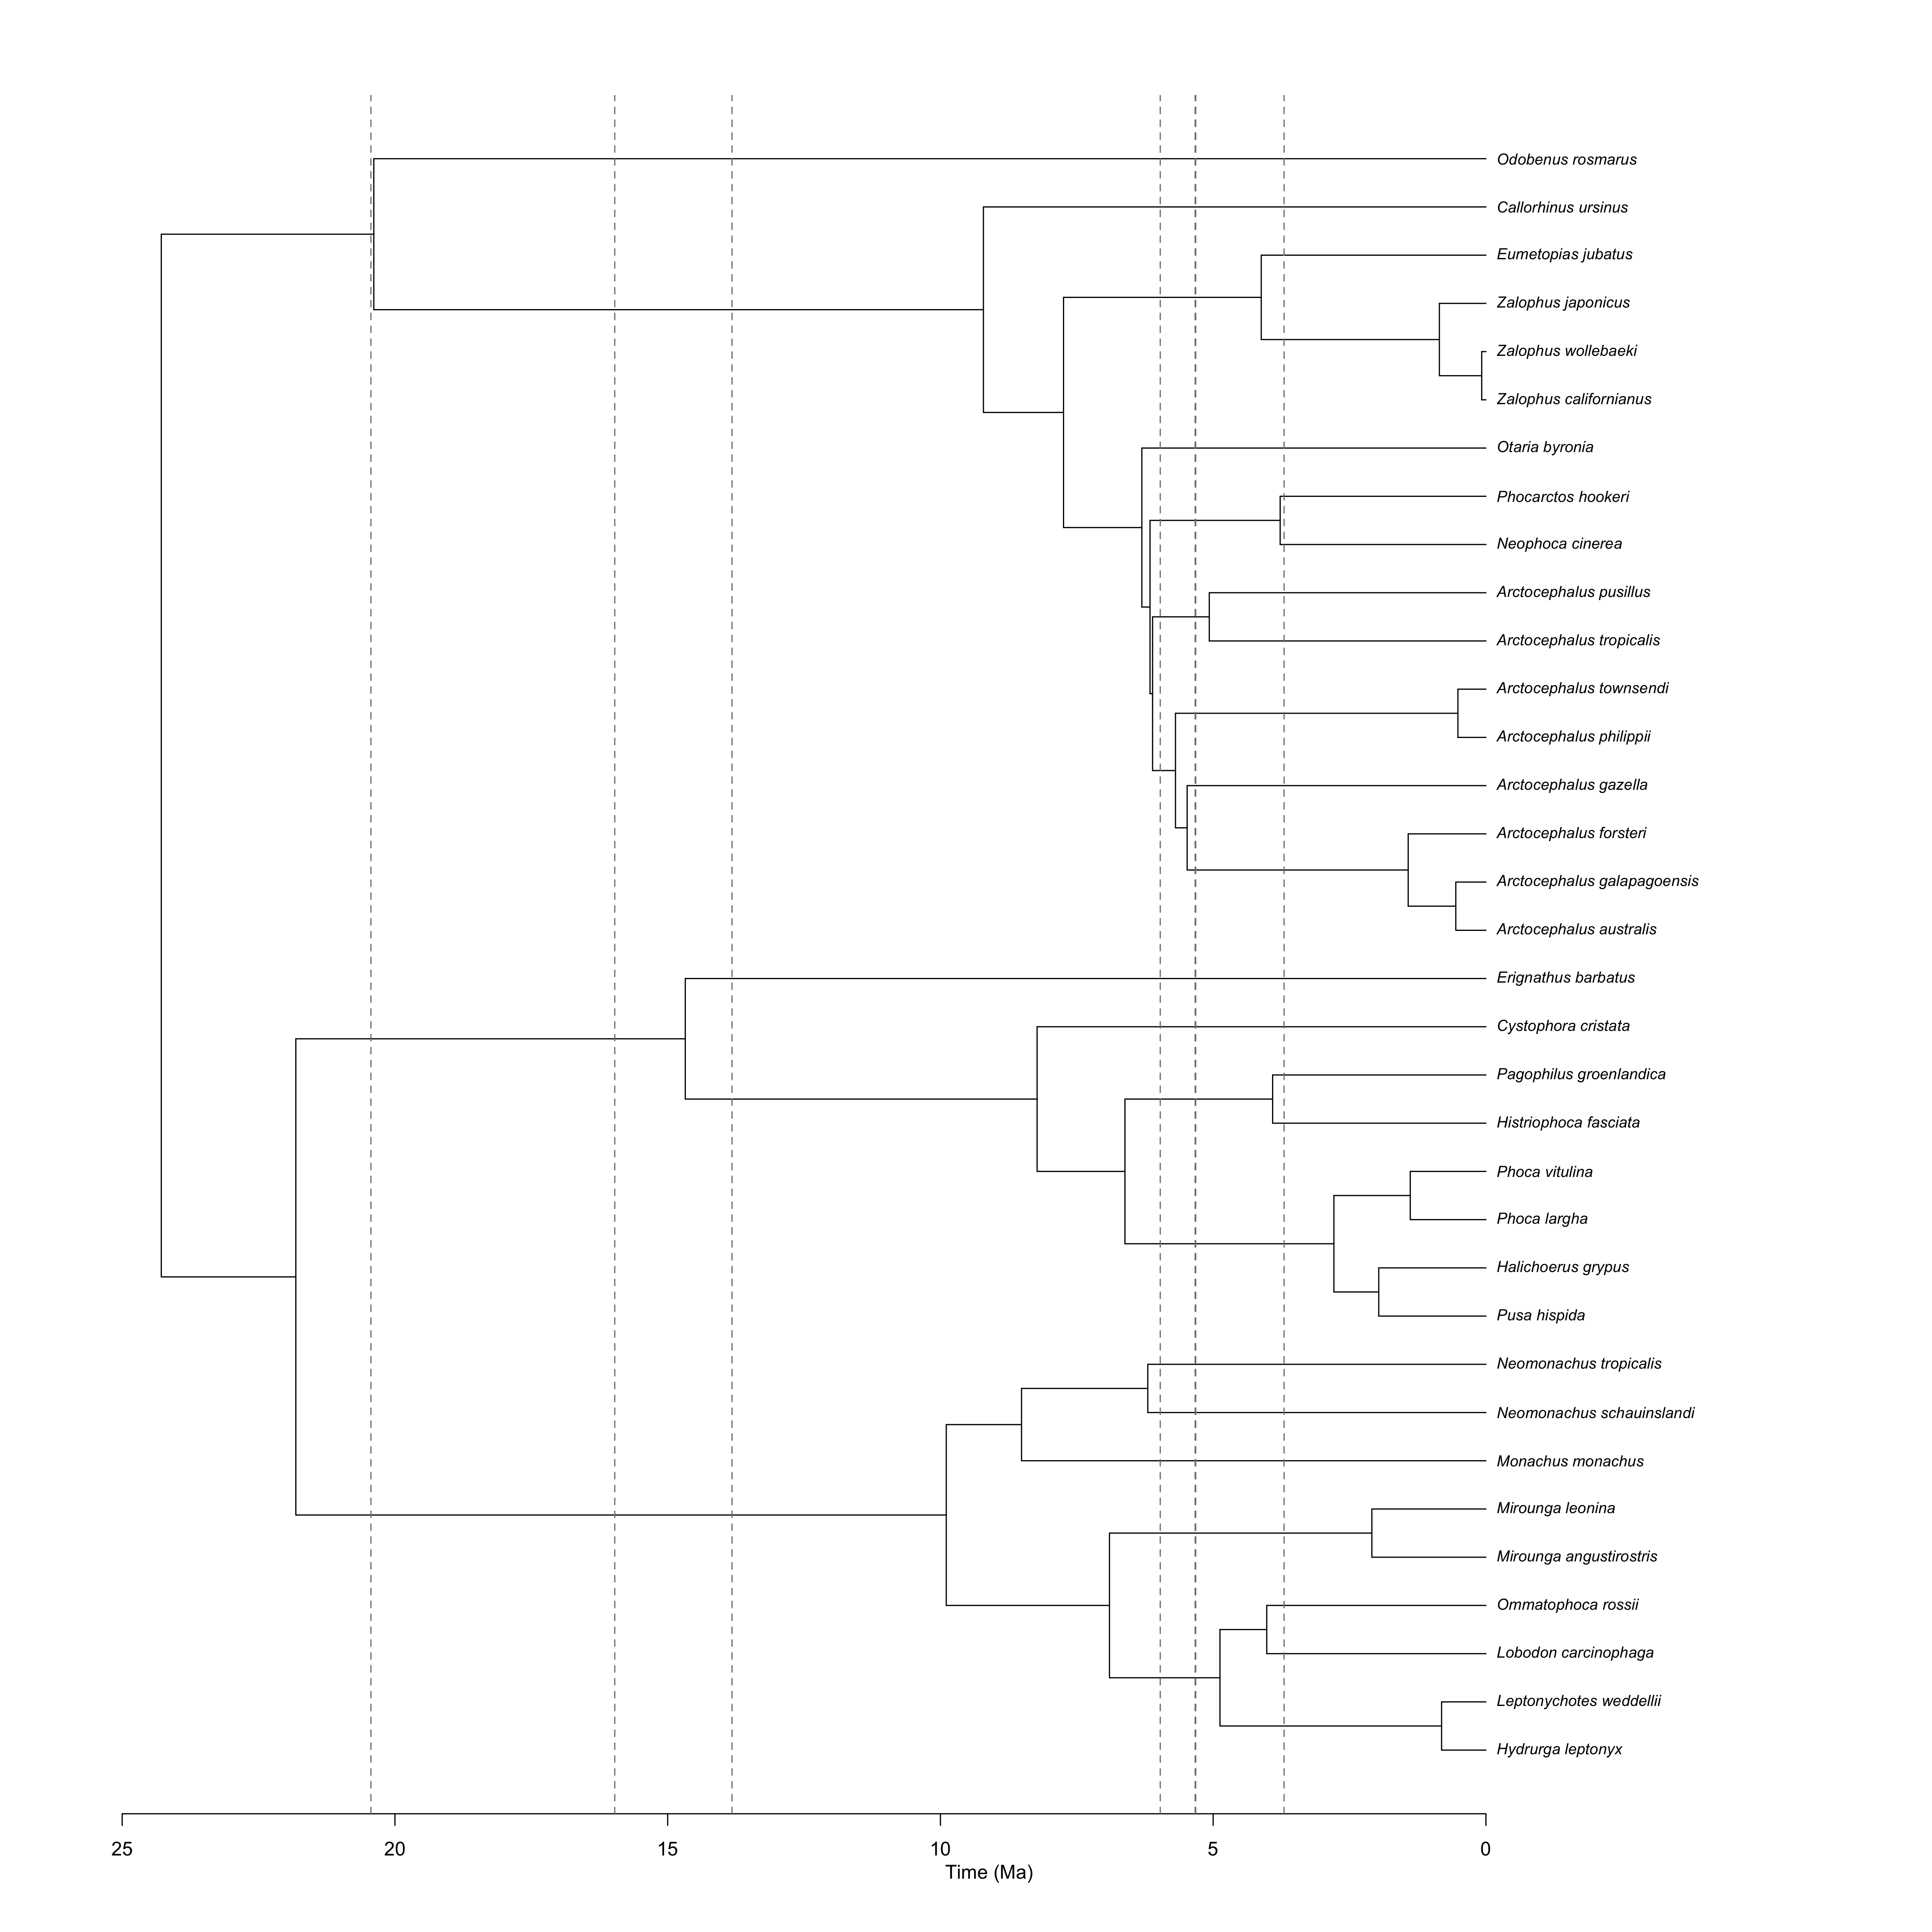
\includegraphics[width = \linewidth]{figures/extant-pinnipeds-tree.png}
  \caption{Phylogeny of extant pinnipeds with taxon names to aid understanding of the following results which have taxon names removed to improve readability.}
  \label{fig-extant-tree}
\end{figure} 

% figure
\begin{figure}[H]
 \centering
  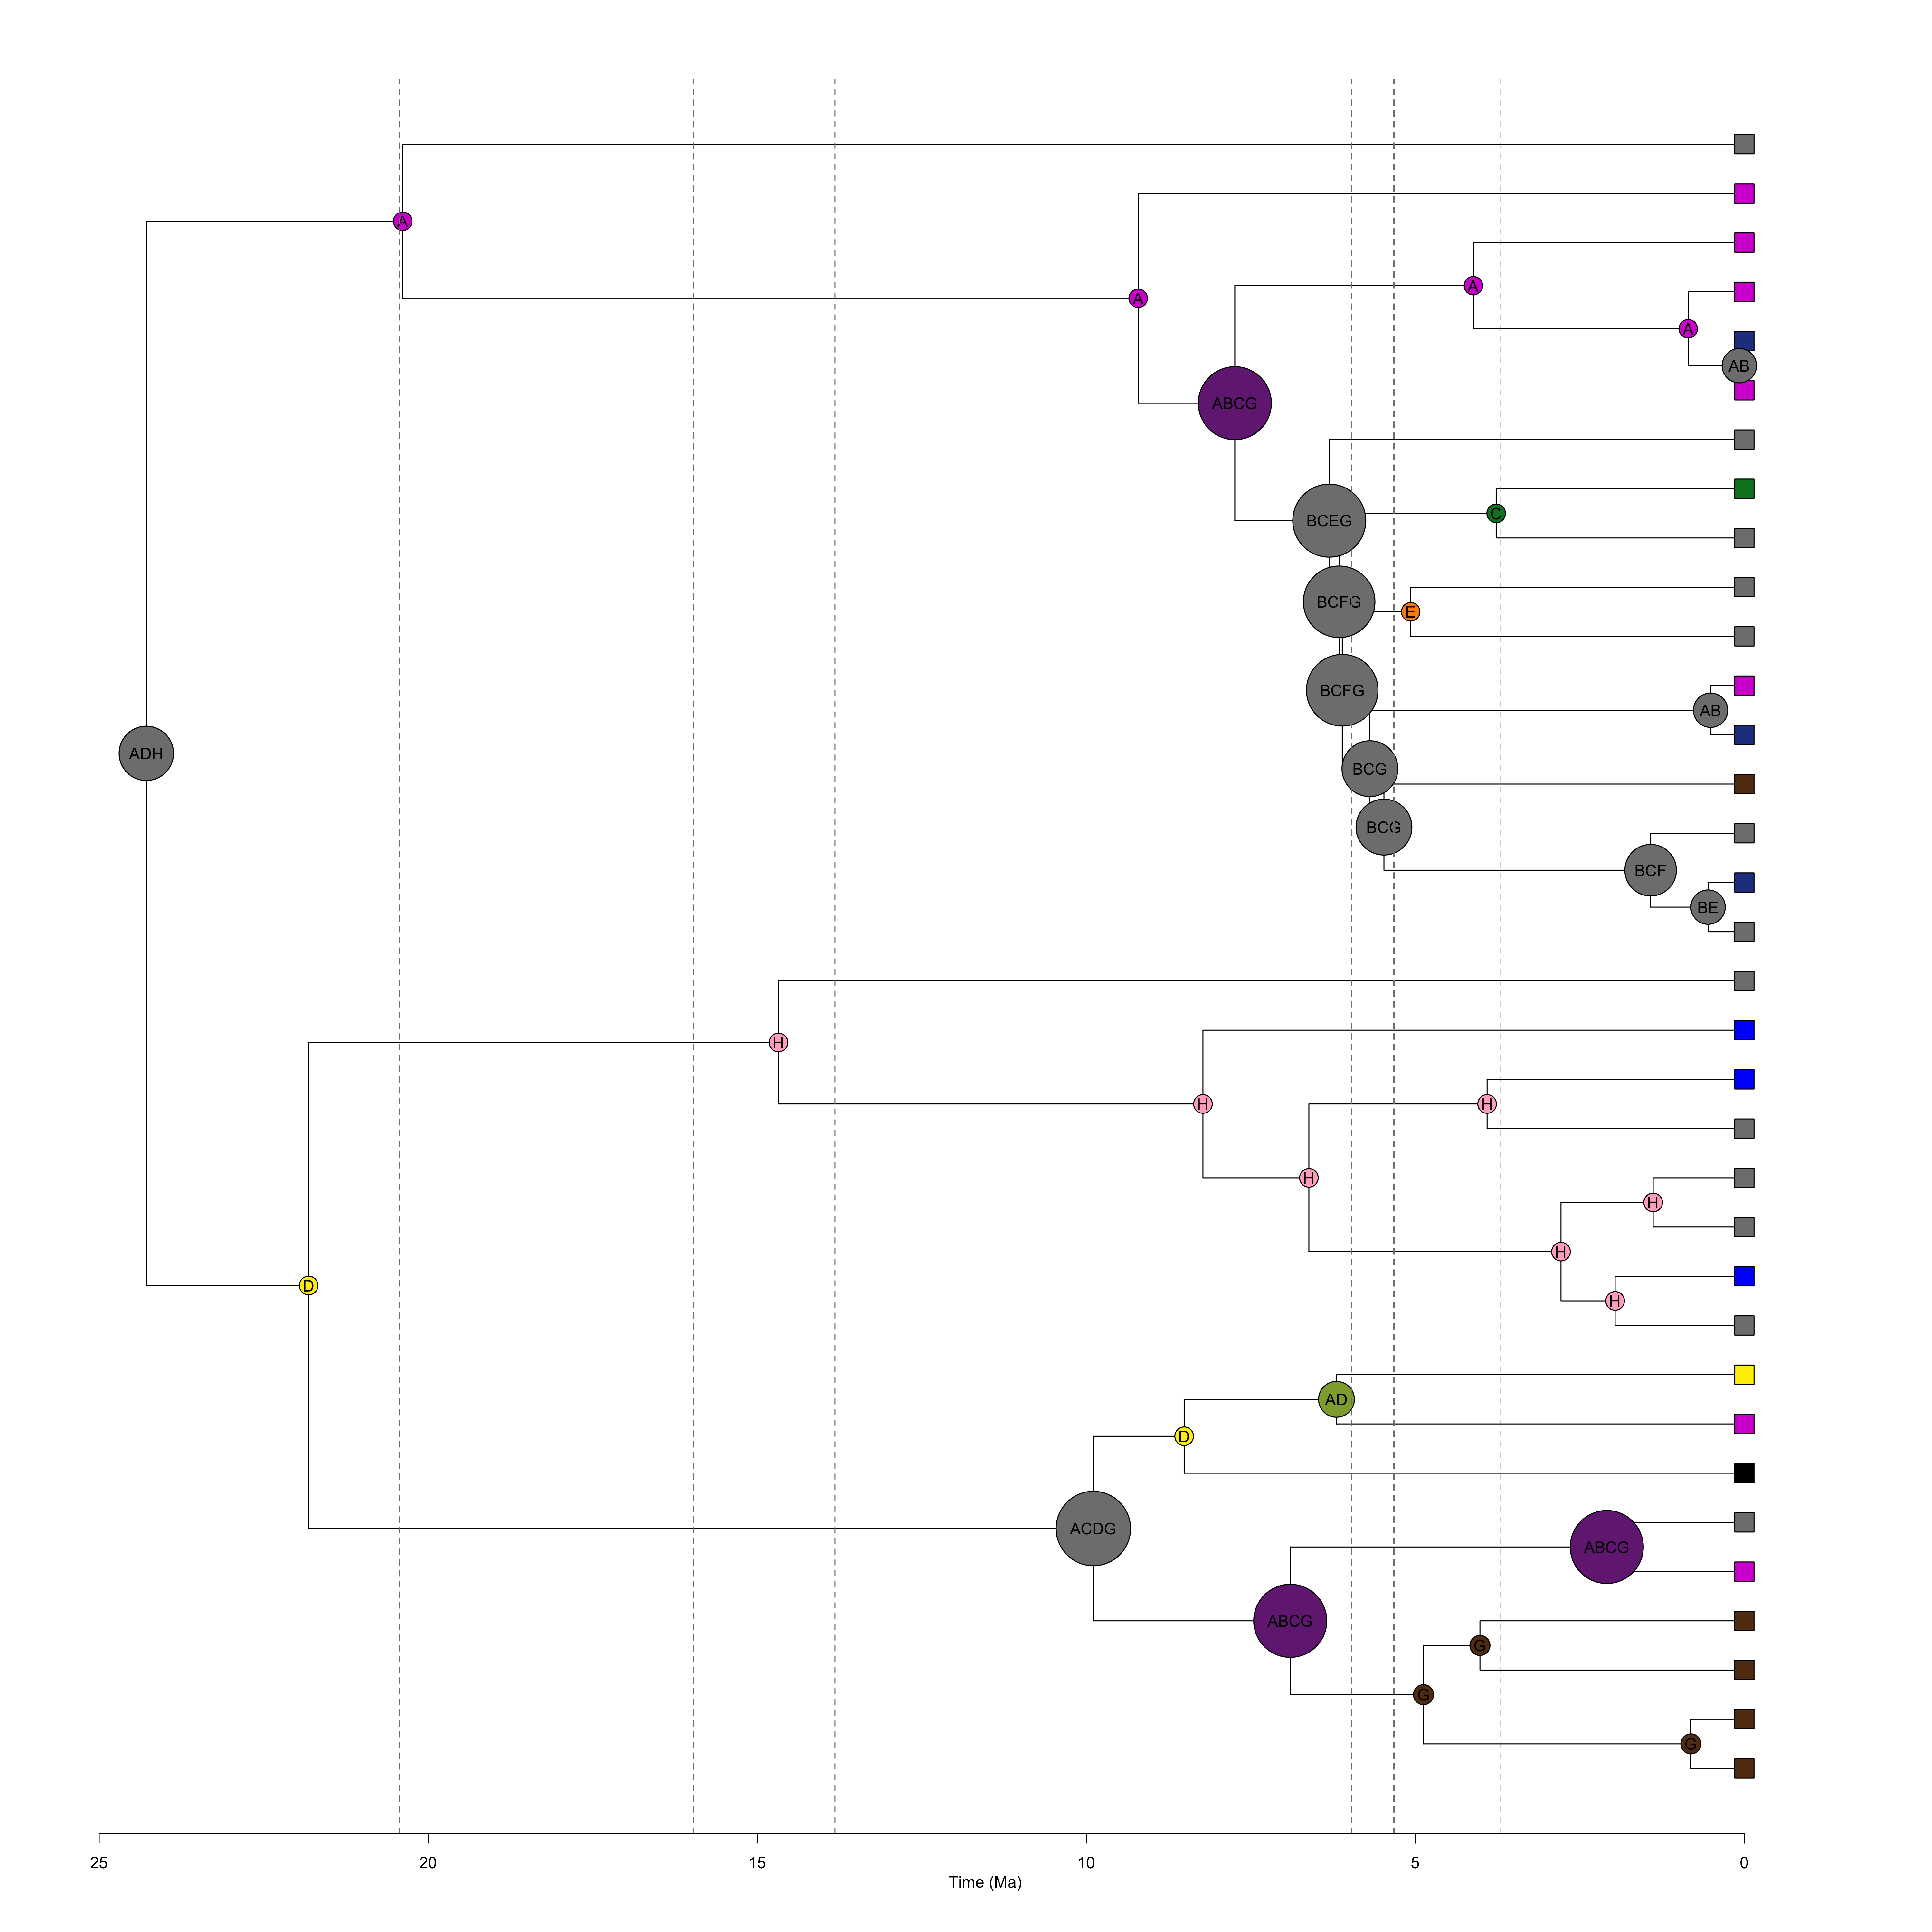
\includegraphics[width = \linewidth]{figures/extant-pinnipeds-DEC-impossible-MLstates.png}
  \caption{Extant pinnipeds only, DEC model, impossible states removed. Nodes show Maximum Likelihood states.}
  \label{fig-extant-dec-ml}
\end{figure} 

% figure
\begin{figure}[H]
 \centering
  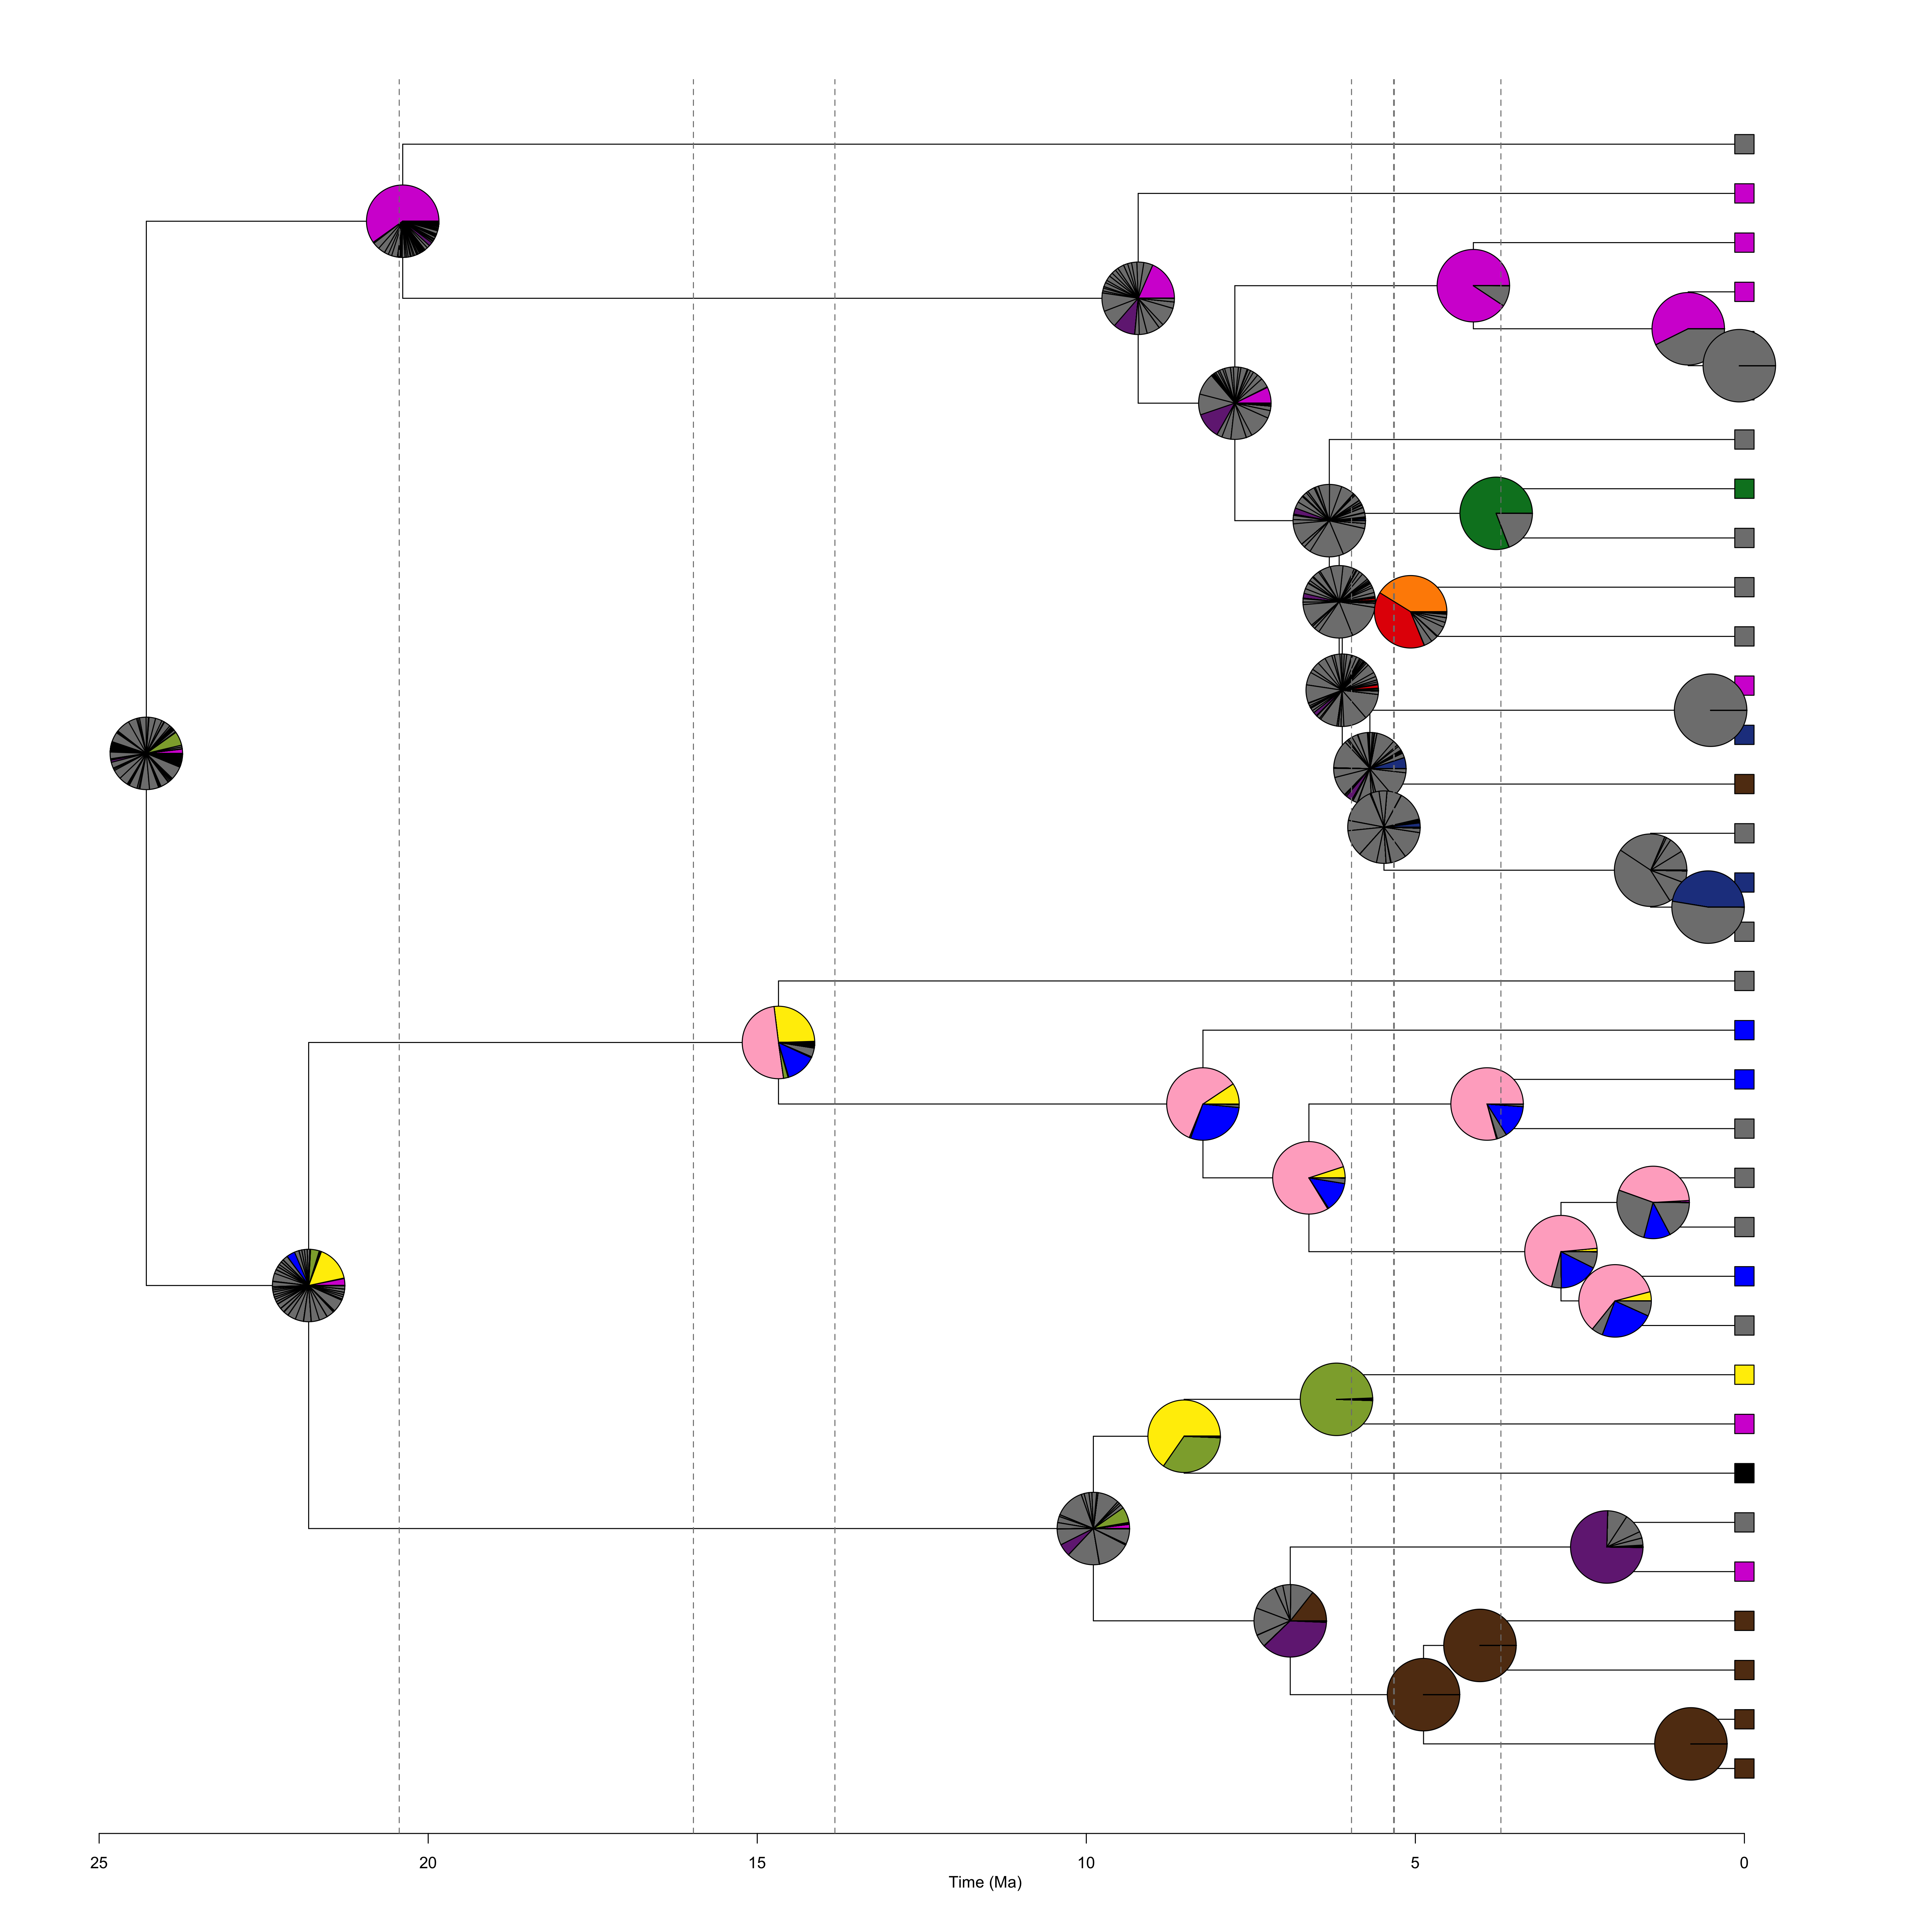
\includegraphics[width = \linewidth]{figures/extant-pinnipeds-DEC-impossible-pies.png}
  \caption{Extant pinnipeds only, DEC model, impossible states removed. Nodes show relative probabilities of each state.}
  \label{fig-extant-dec-pie}
\end{figure} 

% figure
\begin{figure}[H]
 \centering
  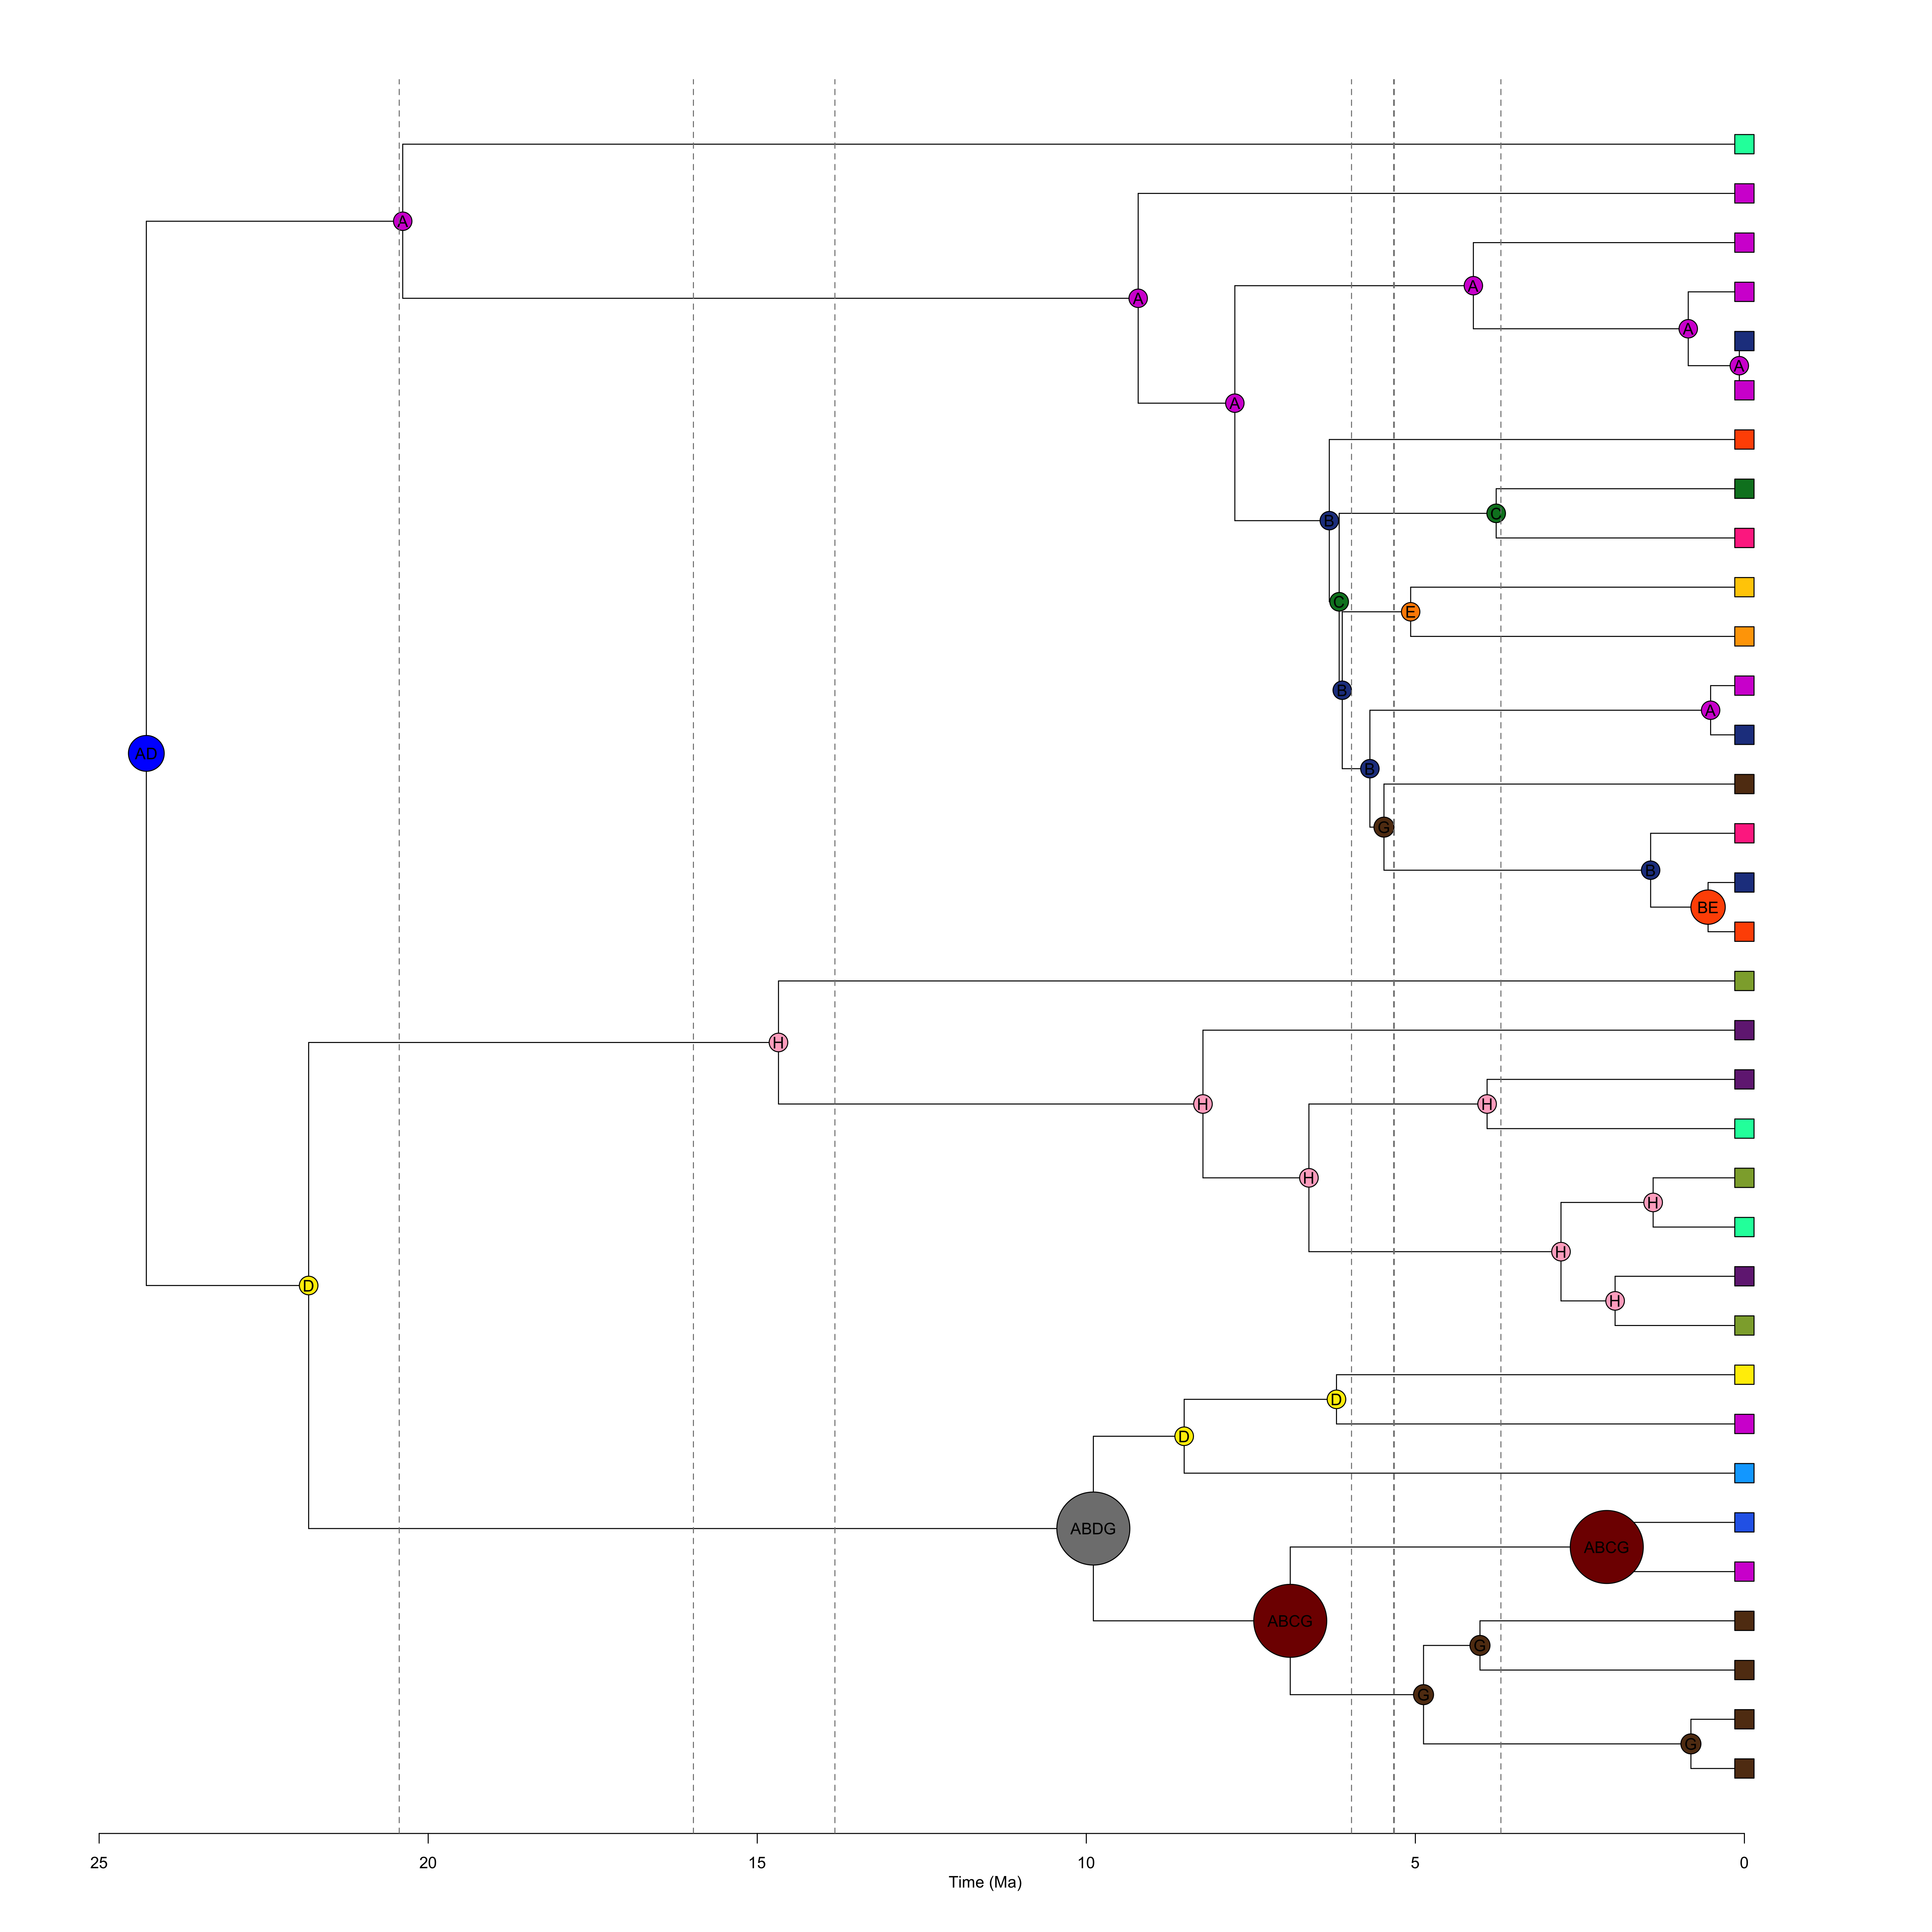
\includegraphics[width = \linewidth]{figures/extant-pinnipeds-DECj-impossible-MLstates.png}
  \caption{Extant pinnipeds only, DEC+J model, impossible states removed. Nodes show Maximum Likelihood states.}
  \label{fig-extant-decj-ml}
\end{figure} 

% figure
\begin{figure}[H]
\centering
  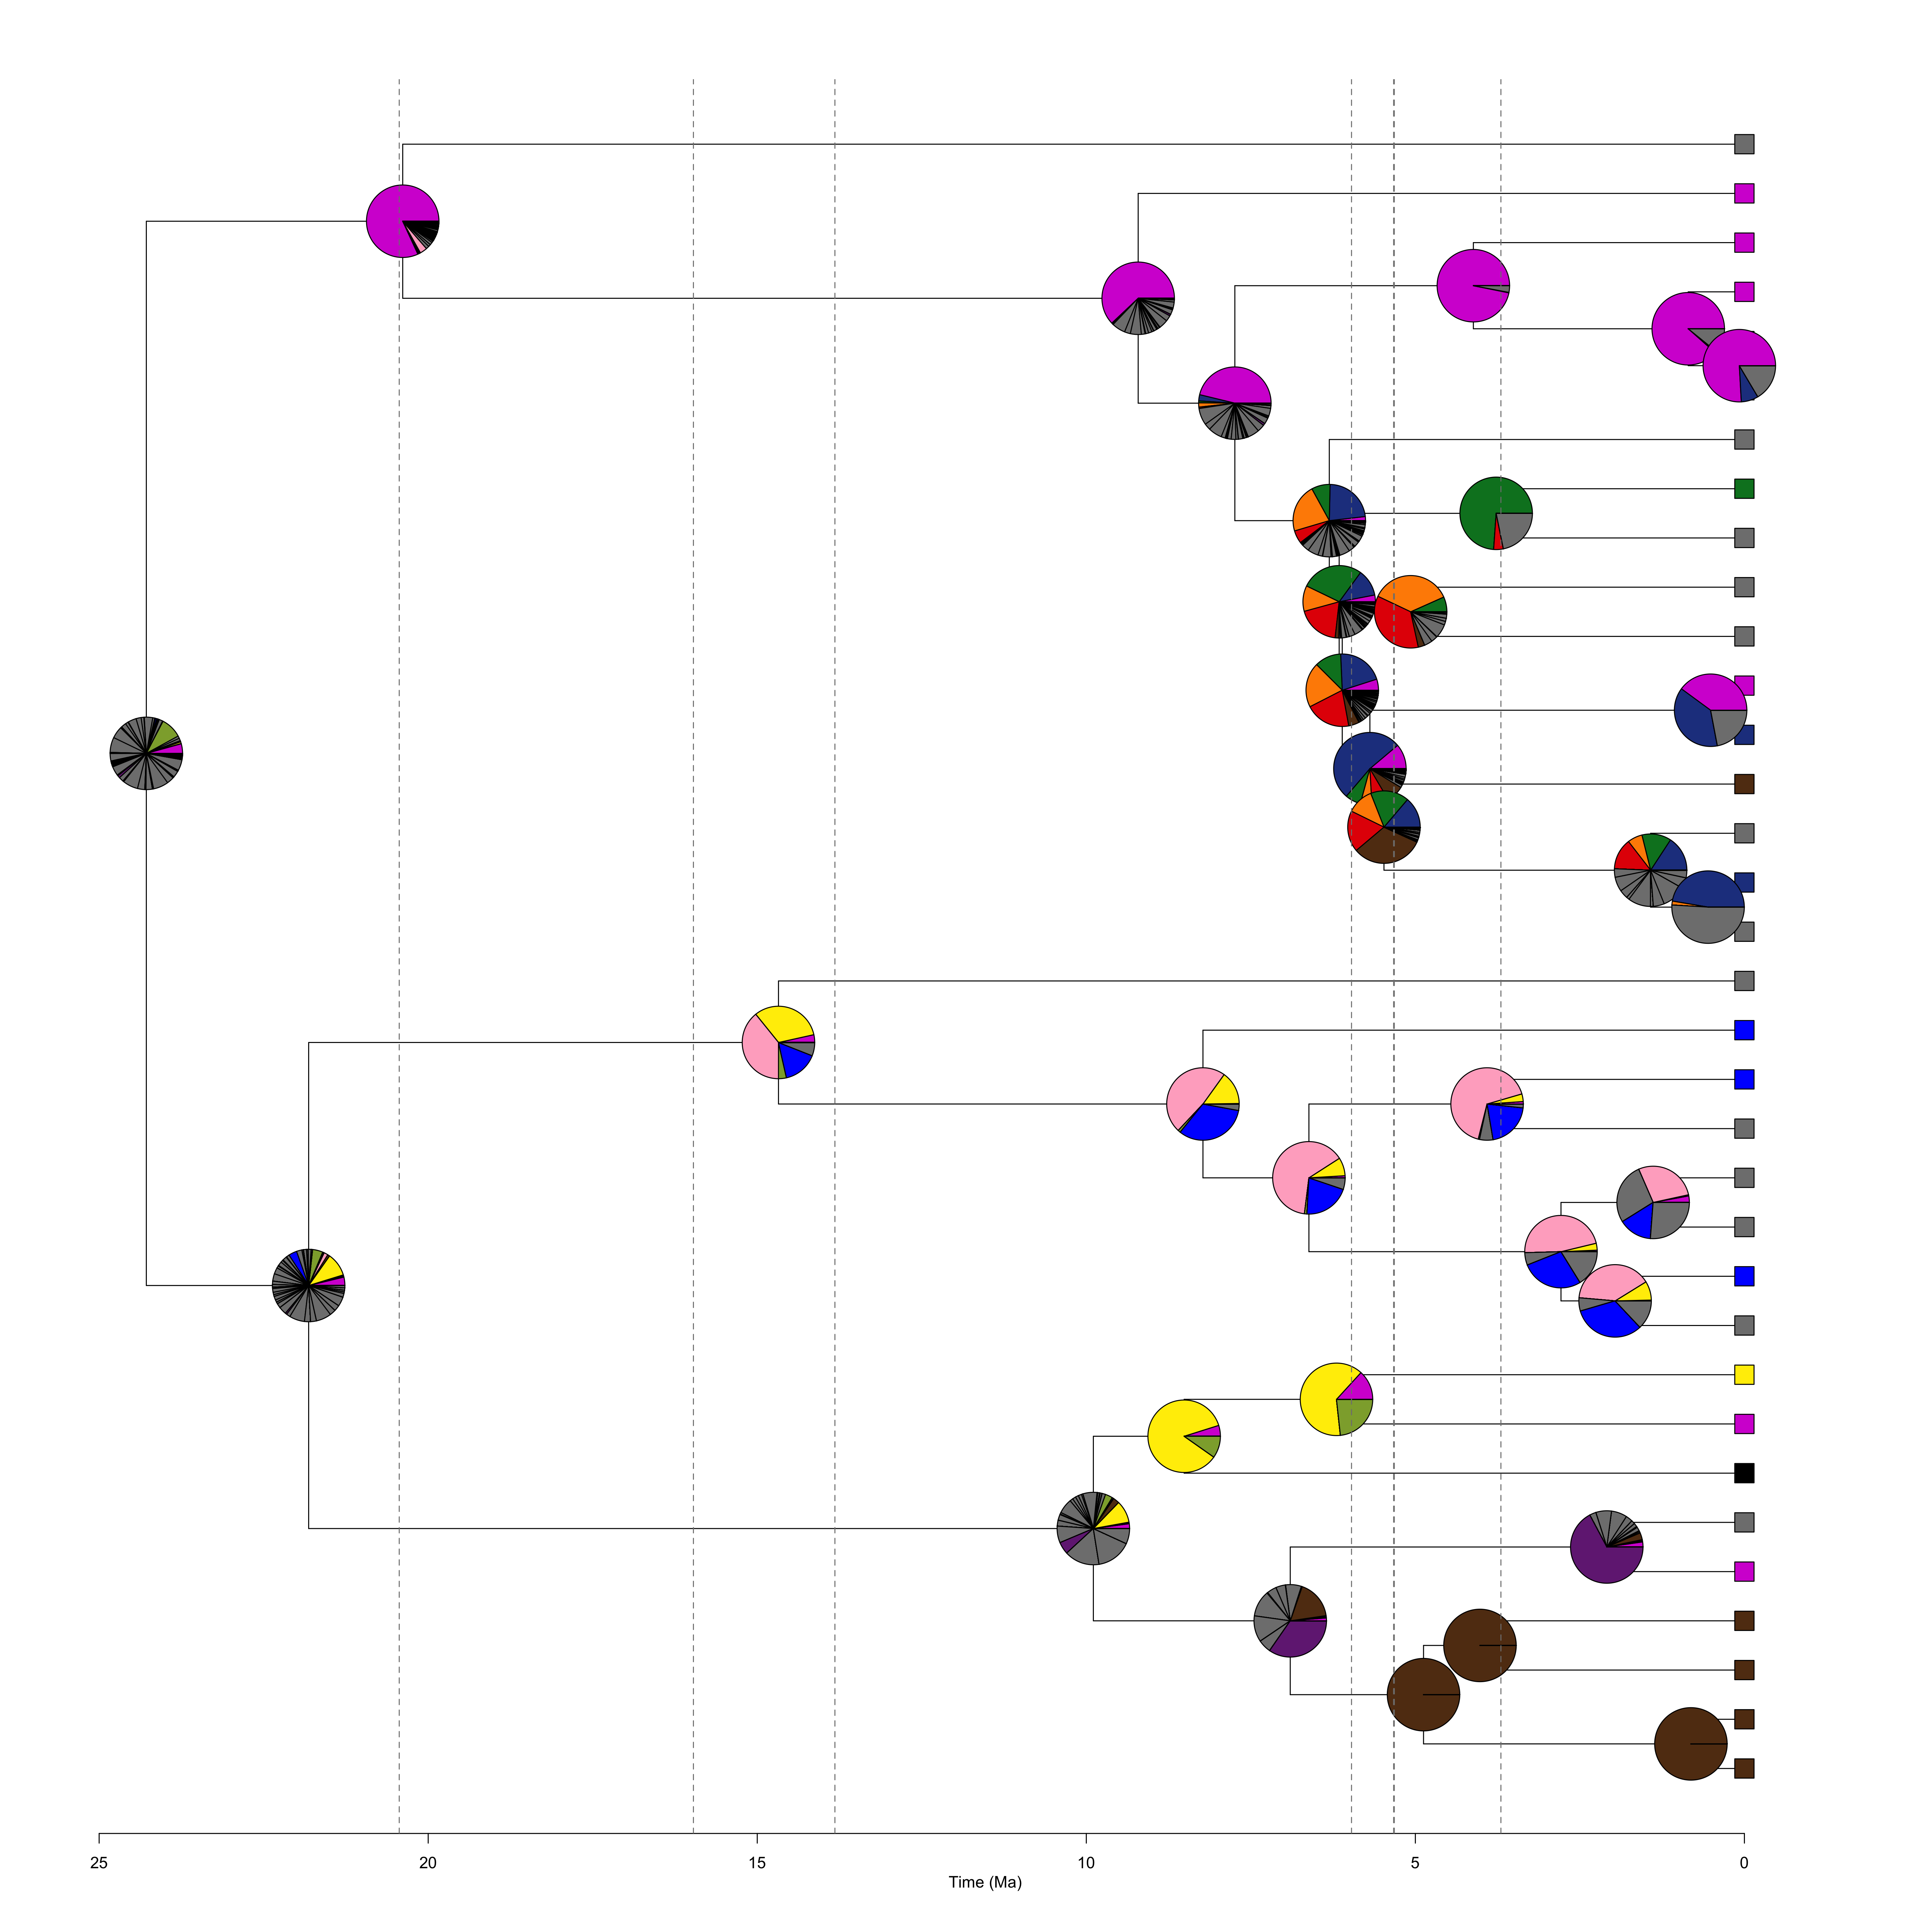
\includegraphics[width = \linewidth]{figures/extant-pinnipeds-DECj-impossible-pies.png}
  \caption{Extant pinnipeds only, DEC+J model, impossible states removed. Nodes show relative probabilities of each state.}
  \label{fig-extant-decj-pie}
\end{figure} 
 
%-----------------------------------------------------------------------------------
\subsubsection{Fossil taxa only}

Ancestral range inference based on the phylogeny of fossil taxa only yielded more confident inference for some nodes than we recovered in analyses based on extant taxa only and, in some cases, approached support recovered from analyses of extant and extinct taxa together (Figures \ref{fig-nodes-all}, \ref{fig-fossil-dec-ml}-\ref{fig-fossil-decj-pie}). The node corresponding to the pinniped crown group is now informed by fossil representatives of Otarioidea on the one hand, and Phocidae plus Desmatophocidae on the other, and is confidently inferred to have occupied the North Pacific, regardless of whether jump dispersal is permitted or not (DEC: P = 0.98, DEC+J: P > 0.99). The common ancestor of Otarioidea is again inferred to have been North Pacific (P > 0.99 under both models), while the common ancestor of crown phocids is here more confidently inferred to have occurred in the North Atlantic (DEC: P = 0.35, DEC+J: P = 0.50) or the North Atlantic plus the Paratethys (DEC: P = 0.47, DEC+J: P = 0.31) due to numerous paratethyan occurrences of crown phocines as well as the devinophocids that fall as sister to crown Phocidae. As in analyses of all taxa, ancestral range inference for Pan-Pinnipedia is ambiguous, with similar levels of support recovered for the same set of possible ranges.   


% figure
\begin{figure}[H]
 \centering
  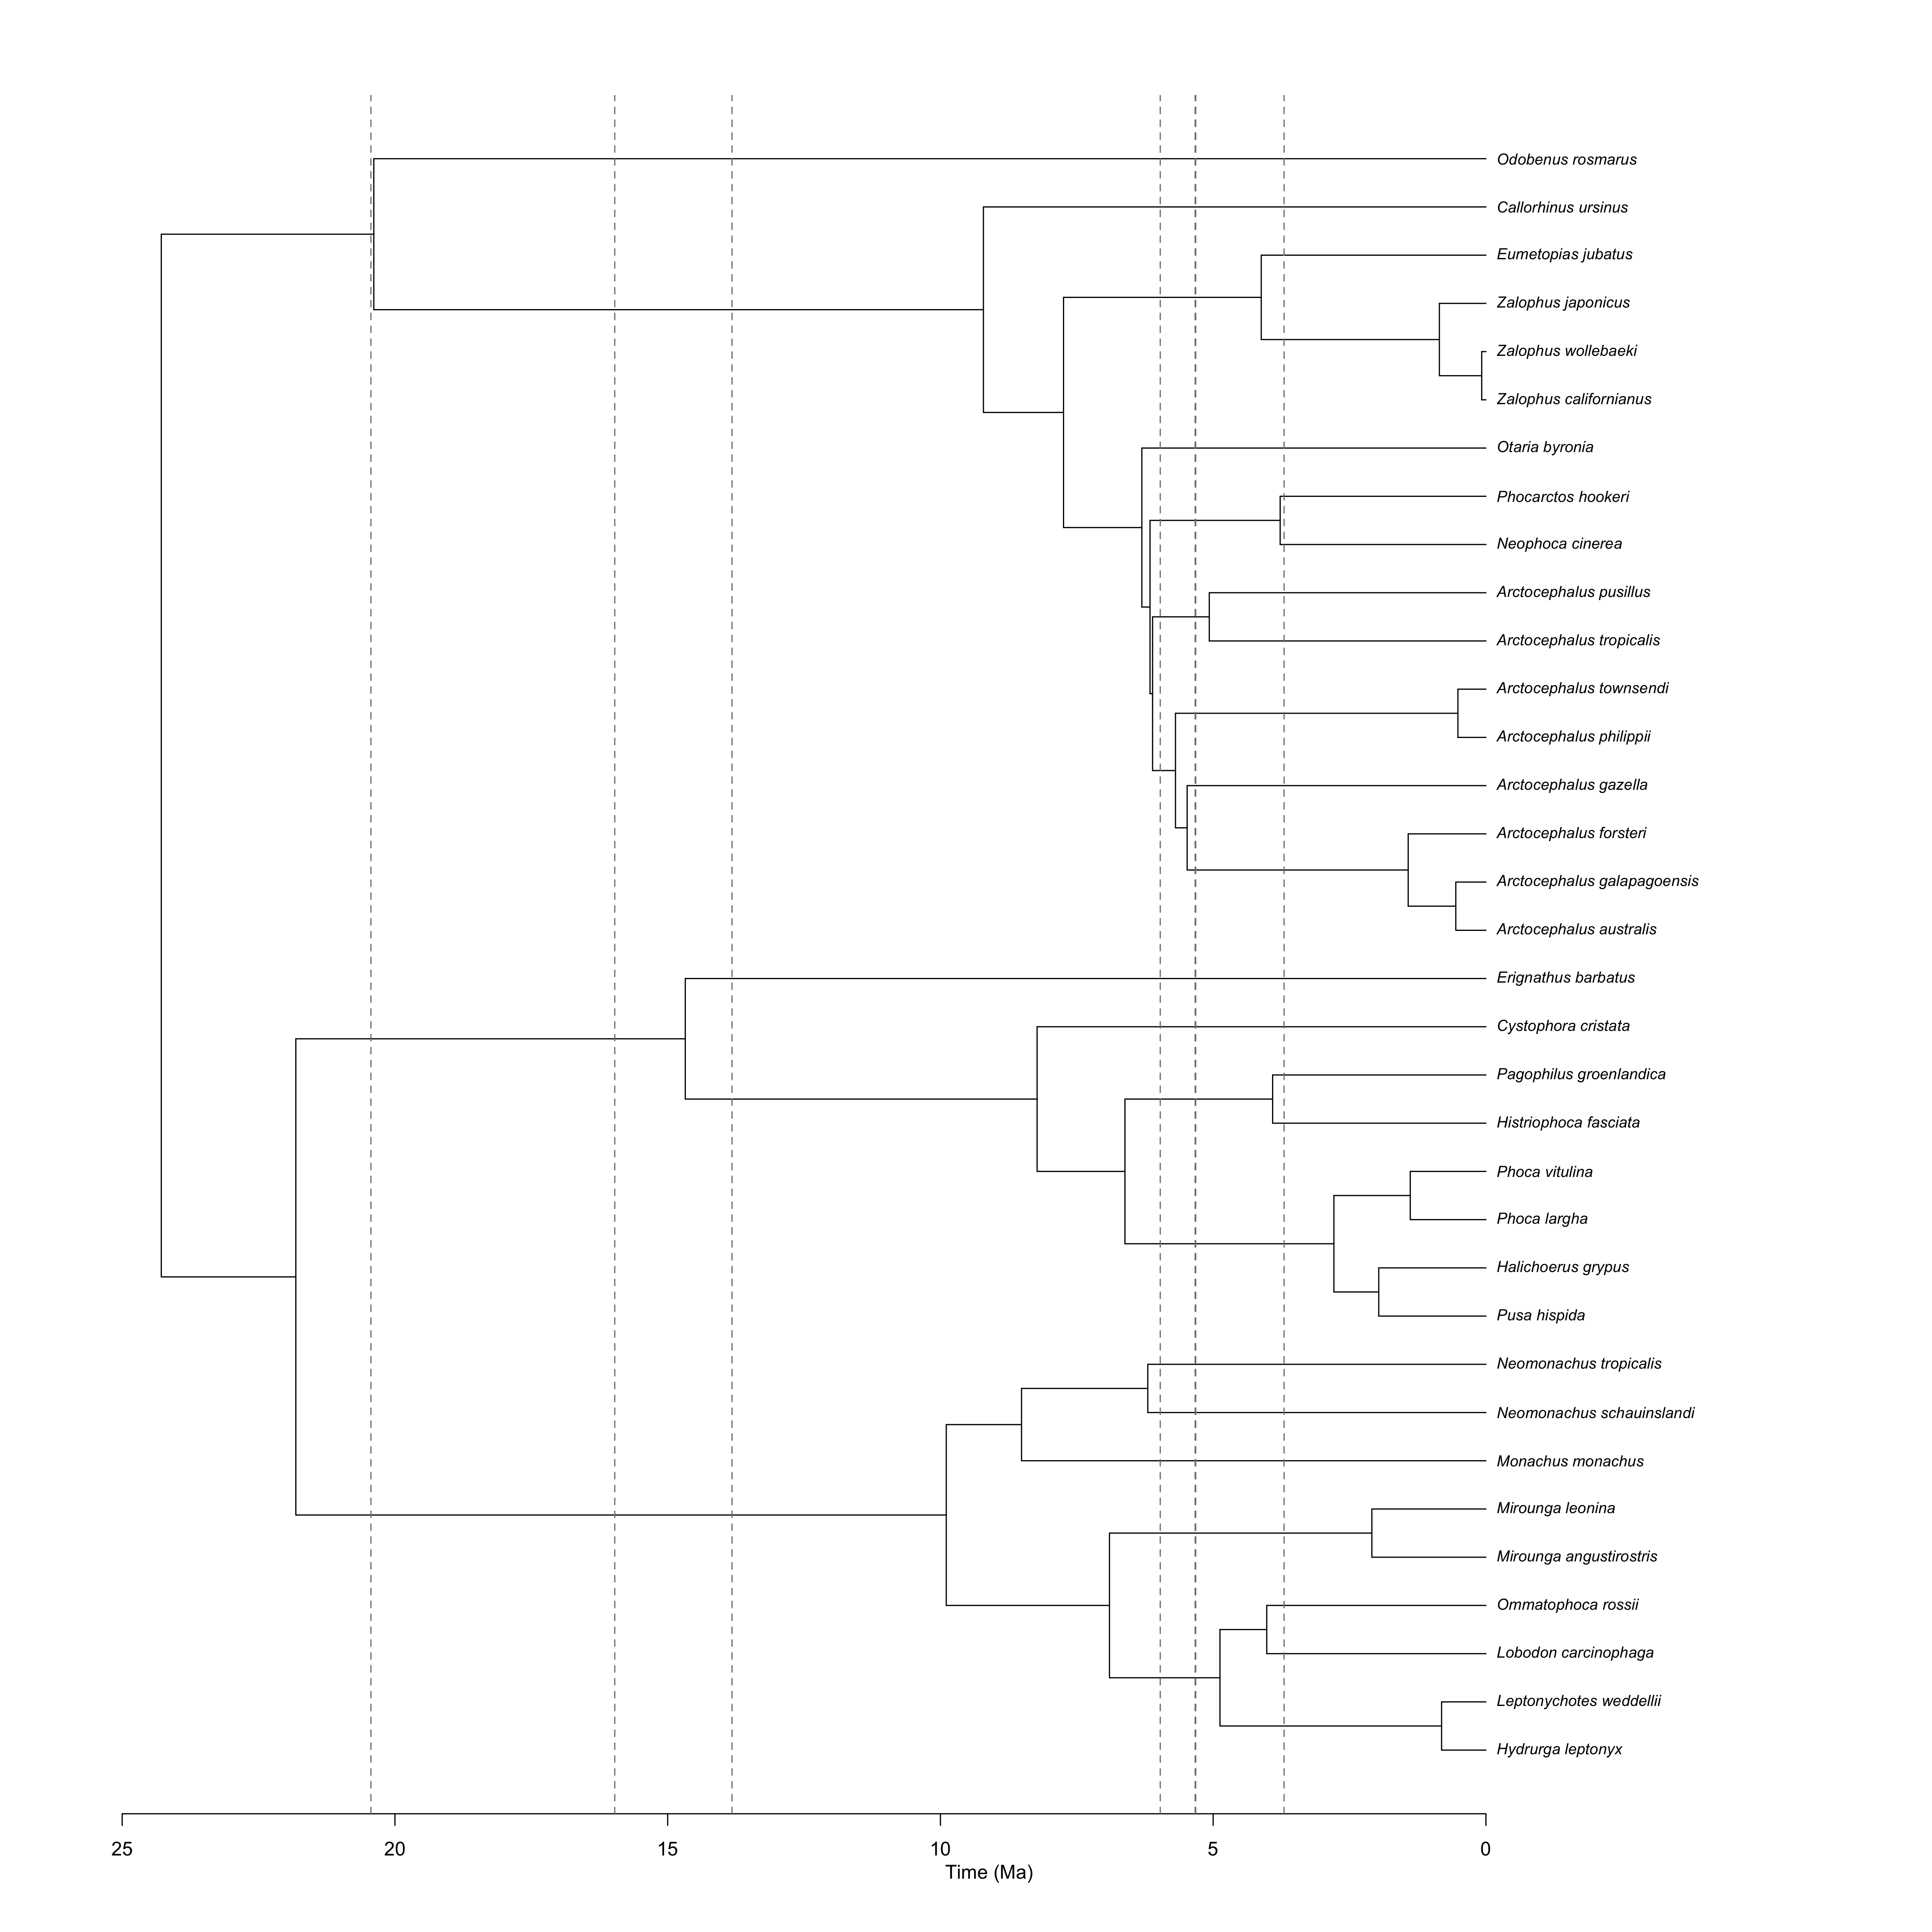
\includegraphics[width = \linewidth]{figures/fossil-pinnipeds-tree.png}
  \caption{Phylogeny of fossil pinnipeds with taxon names to aid understanding of the following results which have taxon names removed to improve readability.}
  \label{fig-fossil-tree}
\end{figure} 

% figure
\begin{figure}[H]
 \centering
  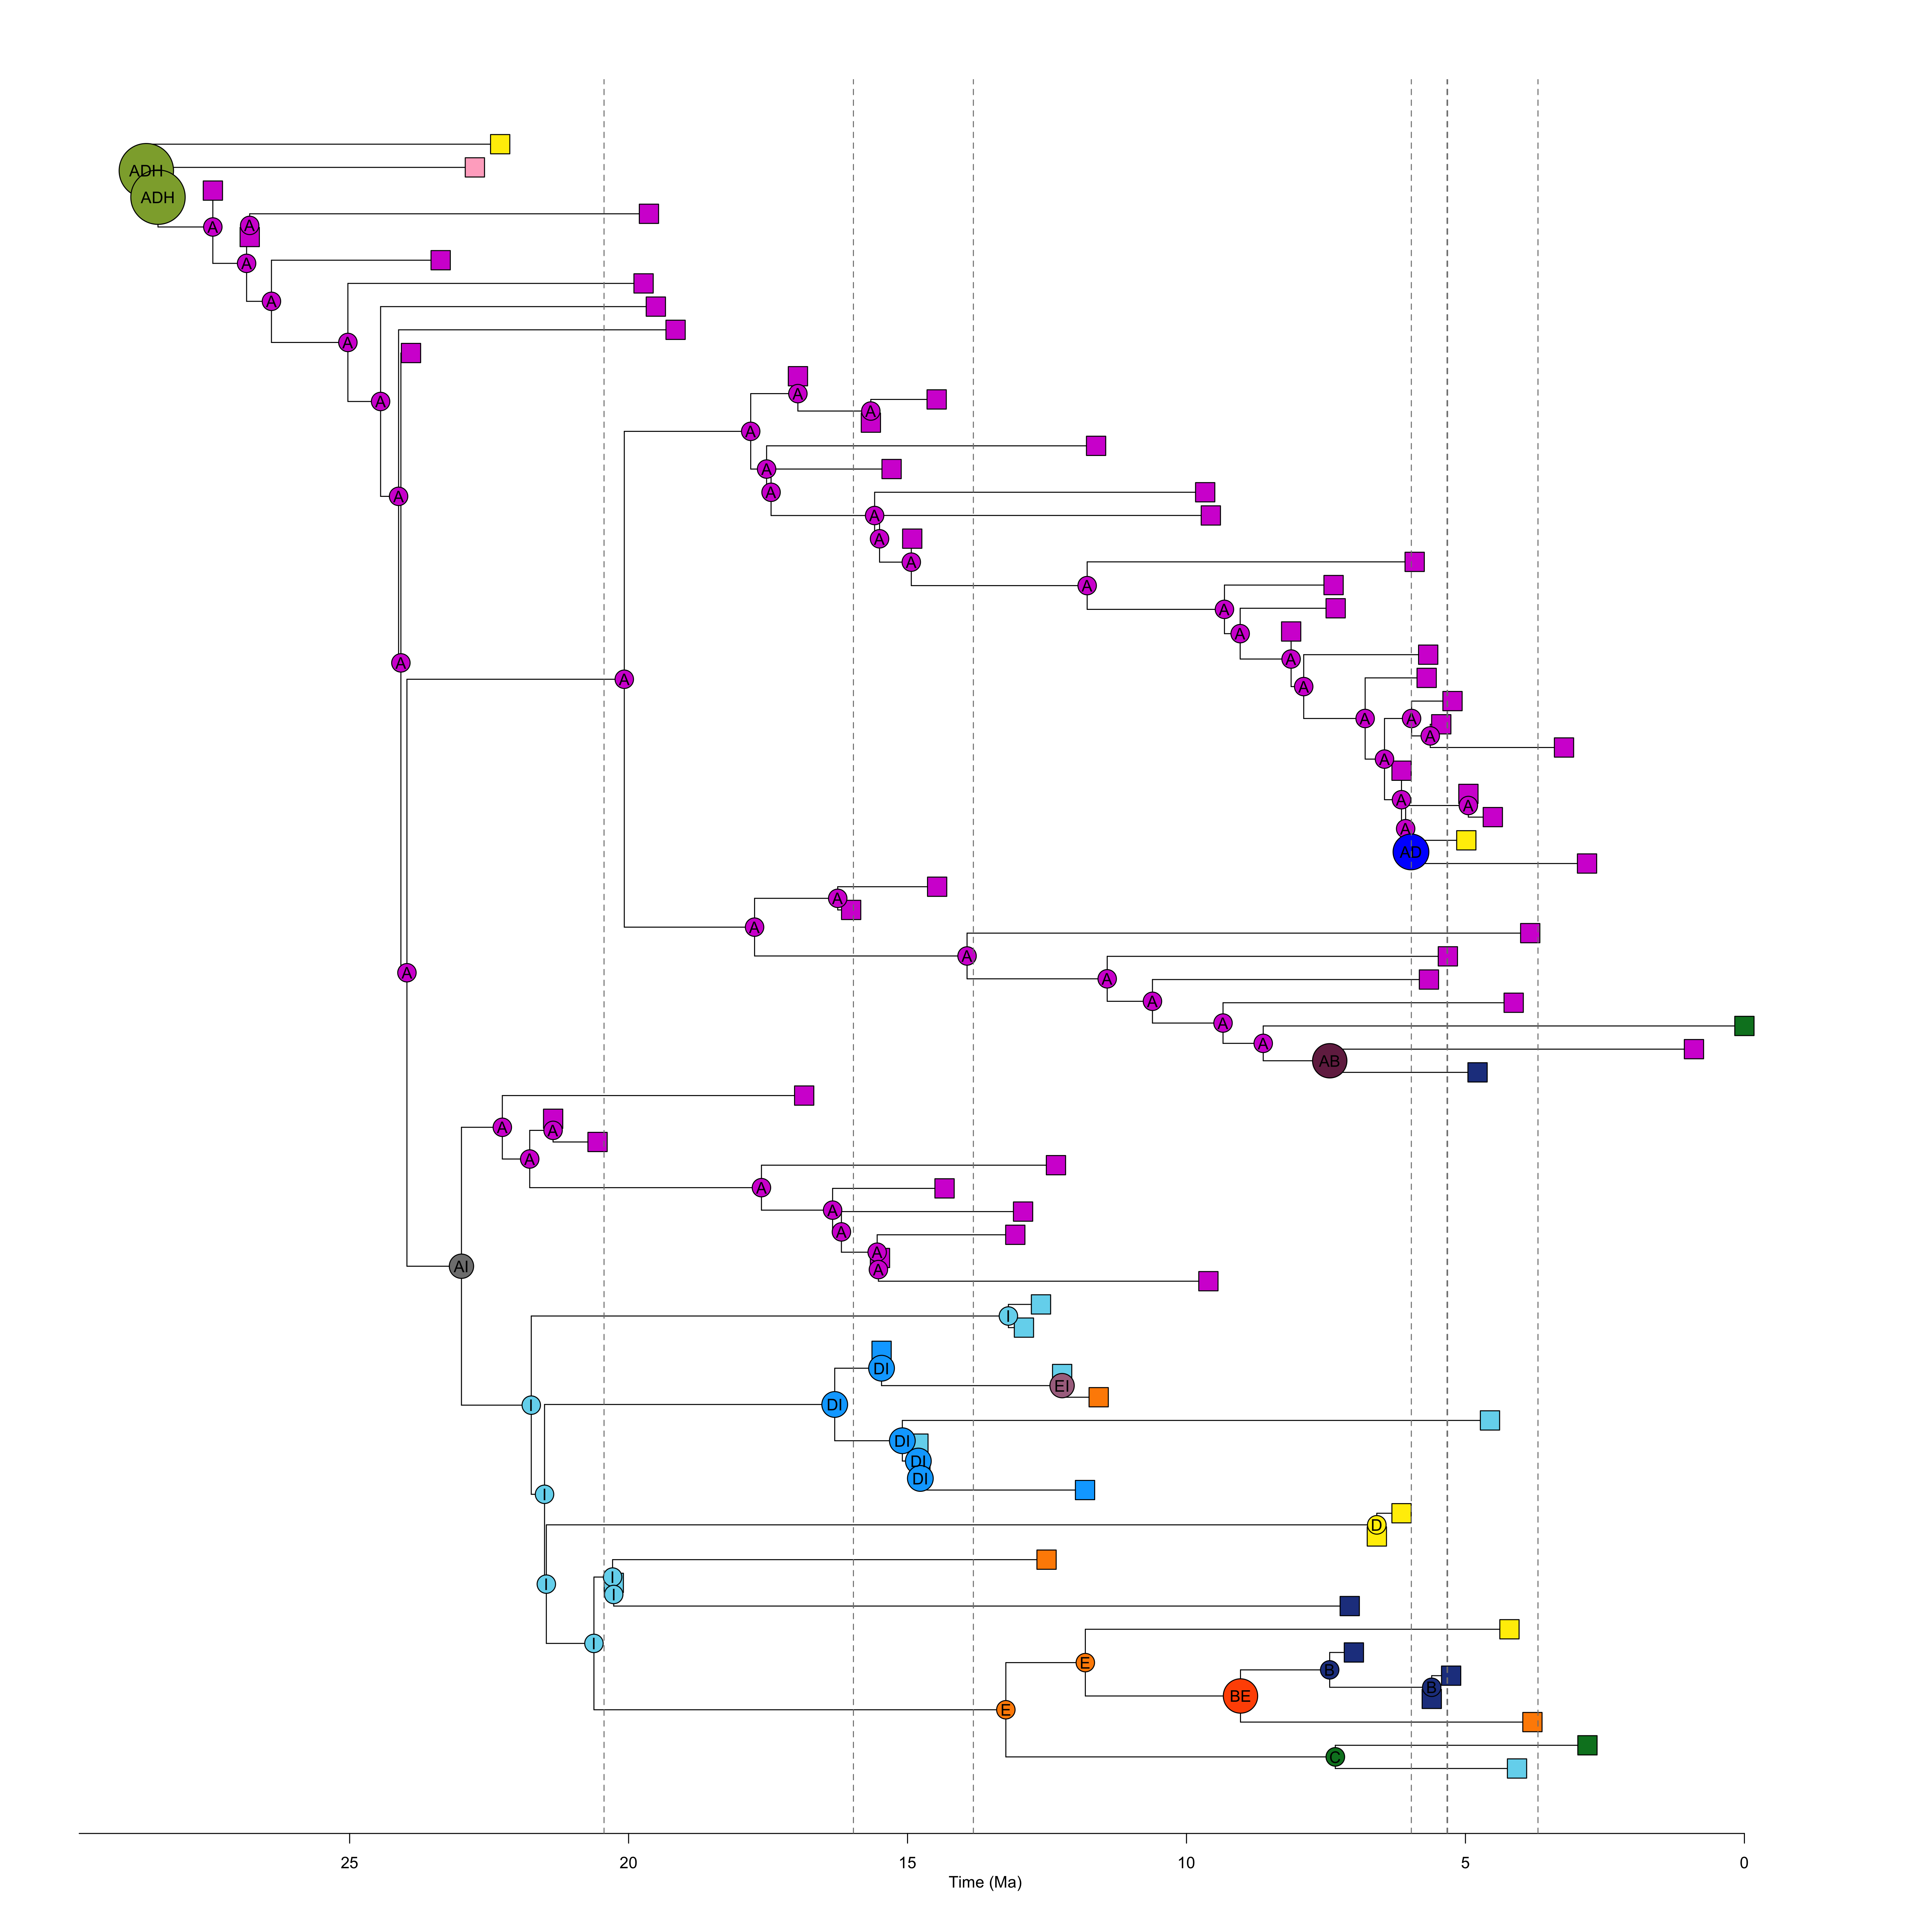
\includegraphics[width = \linewidth]{figures/fossil-pinnipeds-DEC-impossible-MLstates.png}
  \caption{Fossil pinnipeds only, DEC model, impossible states removed. Nodes show Maximum Likelihood states.}
  \label{fig-fossil-dec-ml}
\end{figure} 

% figure
\begin{figure}[H]
 \centering
  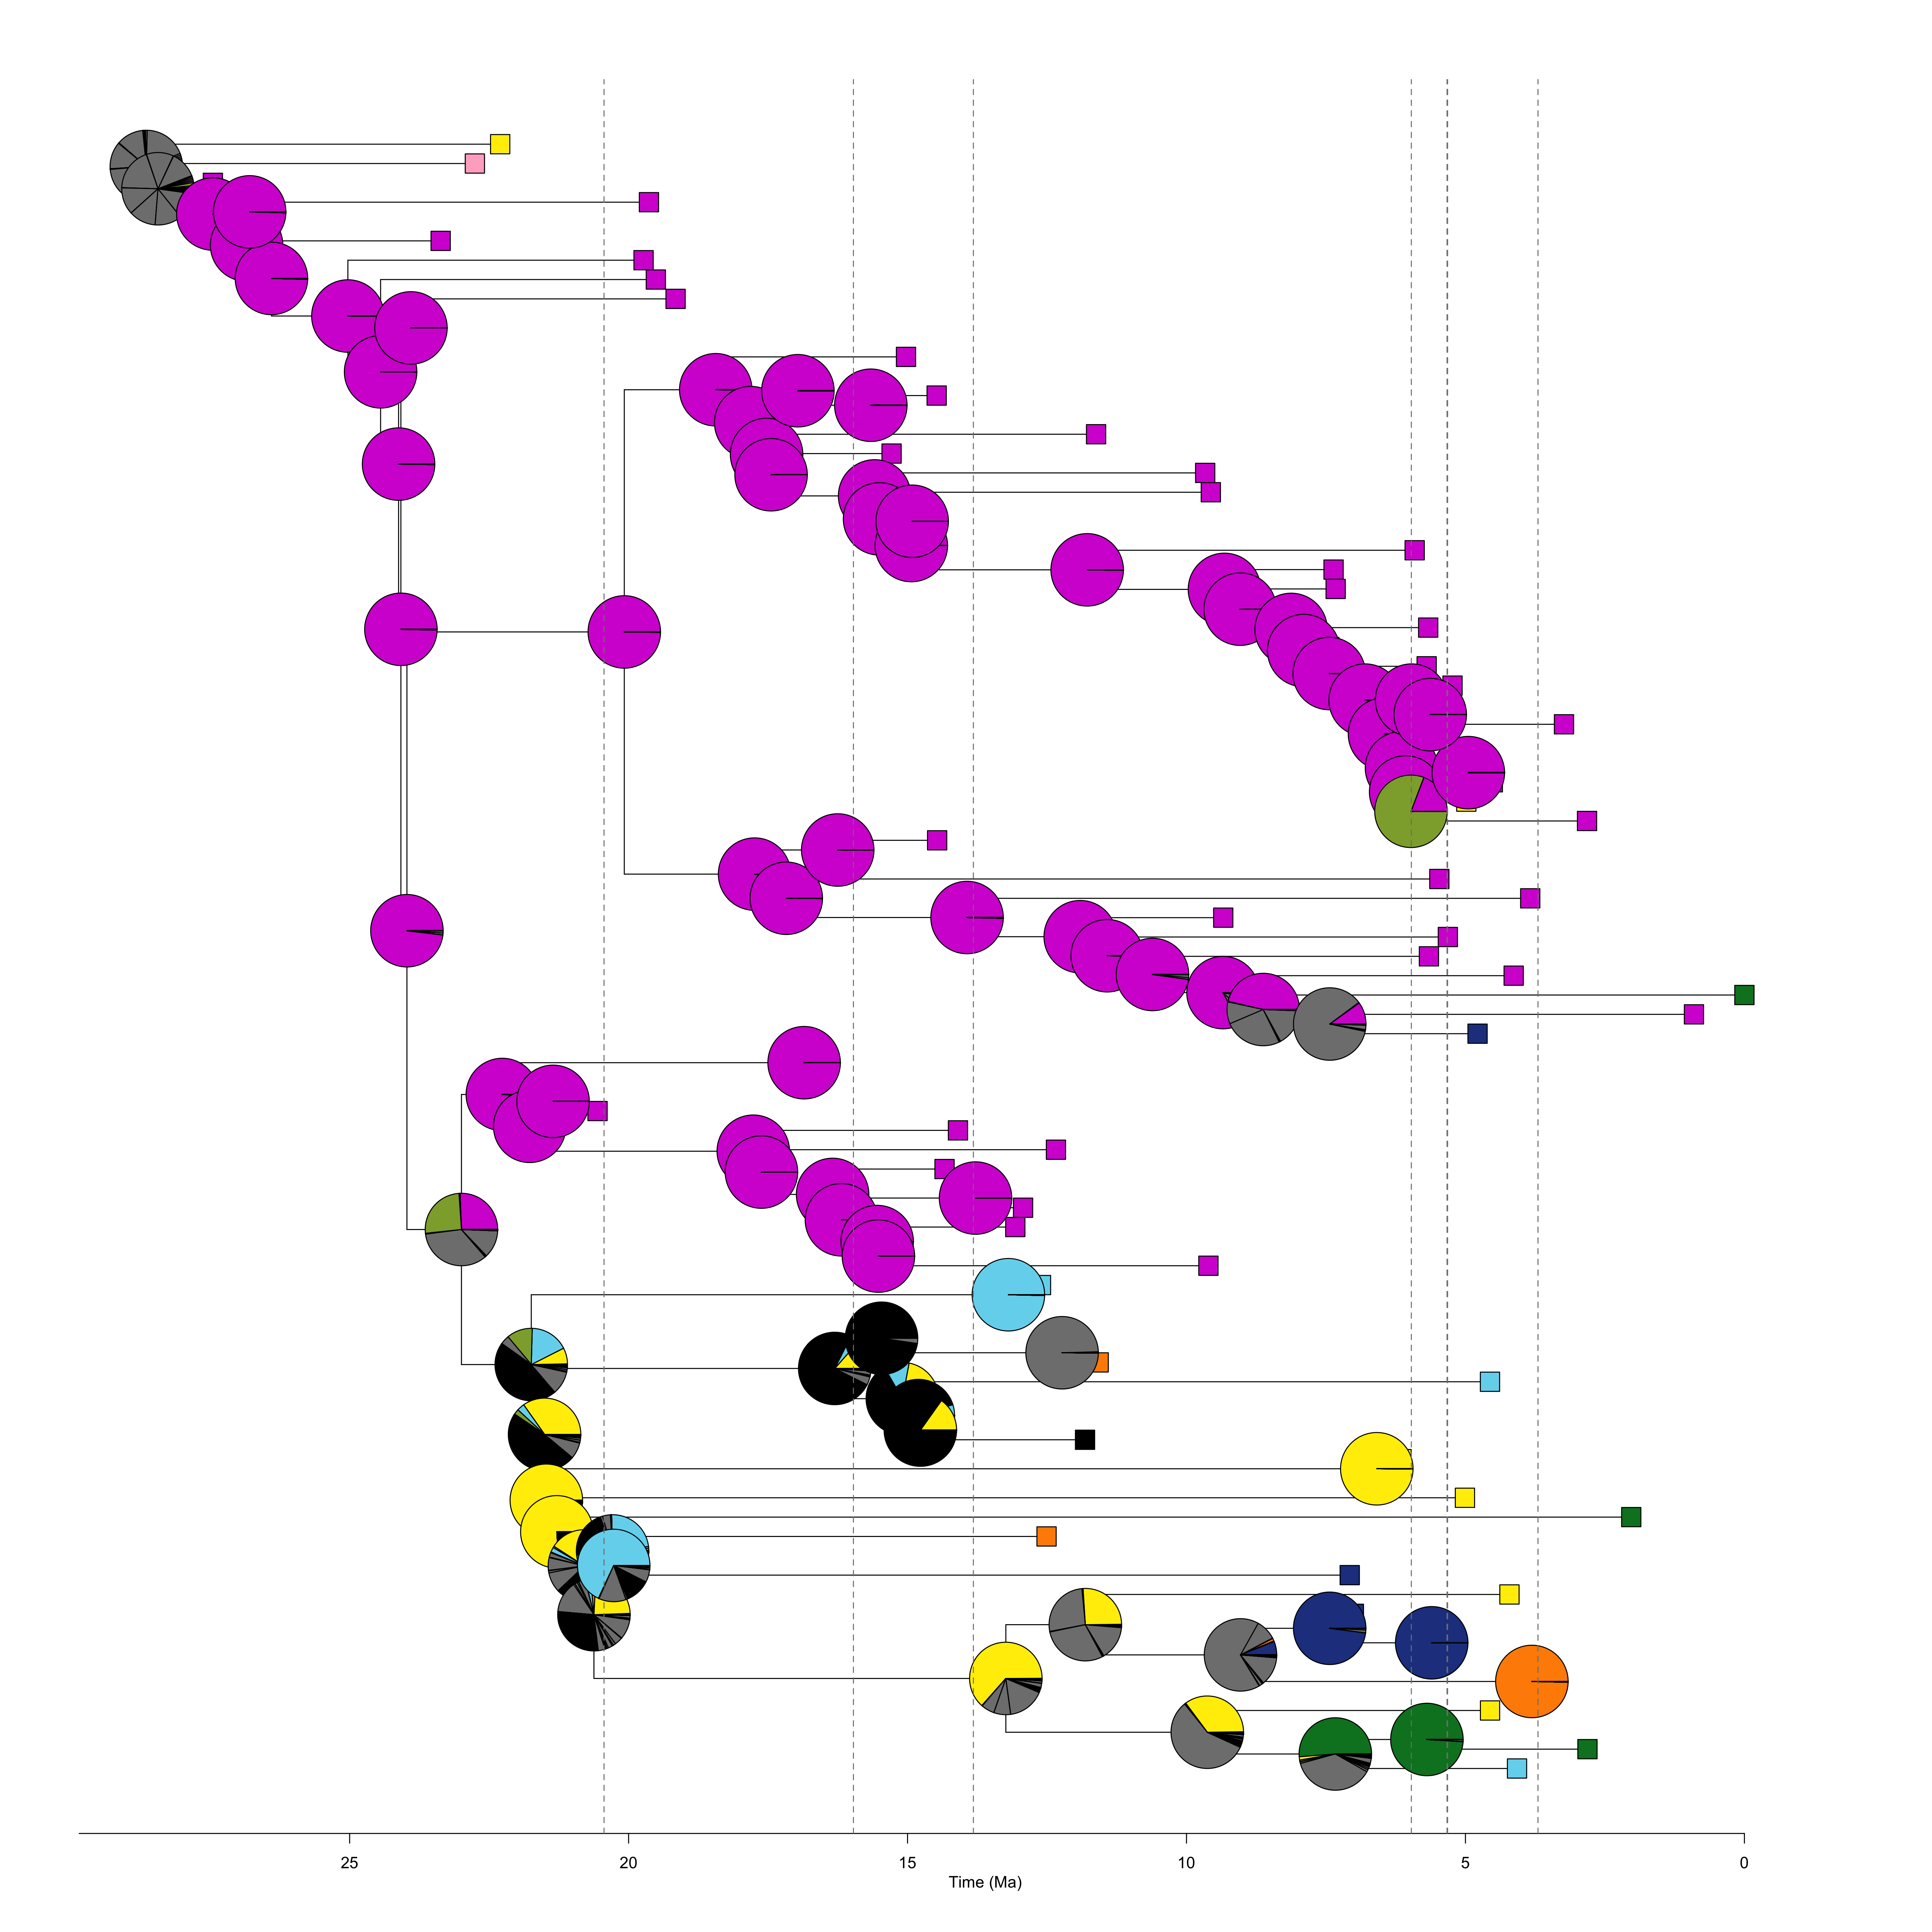
\includegraphics[width = \linewidth]{figures/fossil-pinnipeds-DEC-impossible-pies.png}
  \caption{Fossil pinnipeds only, DEC model, impossible states removed. Nodes show relative probabilities of each state.}
  \label{fig-fossil-dec-pie}
\end{figure} 

% figure
\begin{figure}[H]
 \centering
  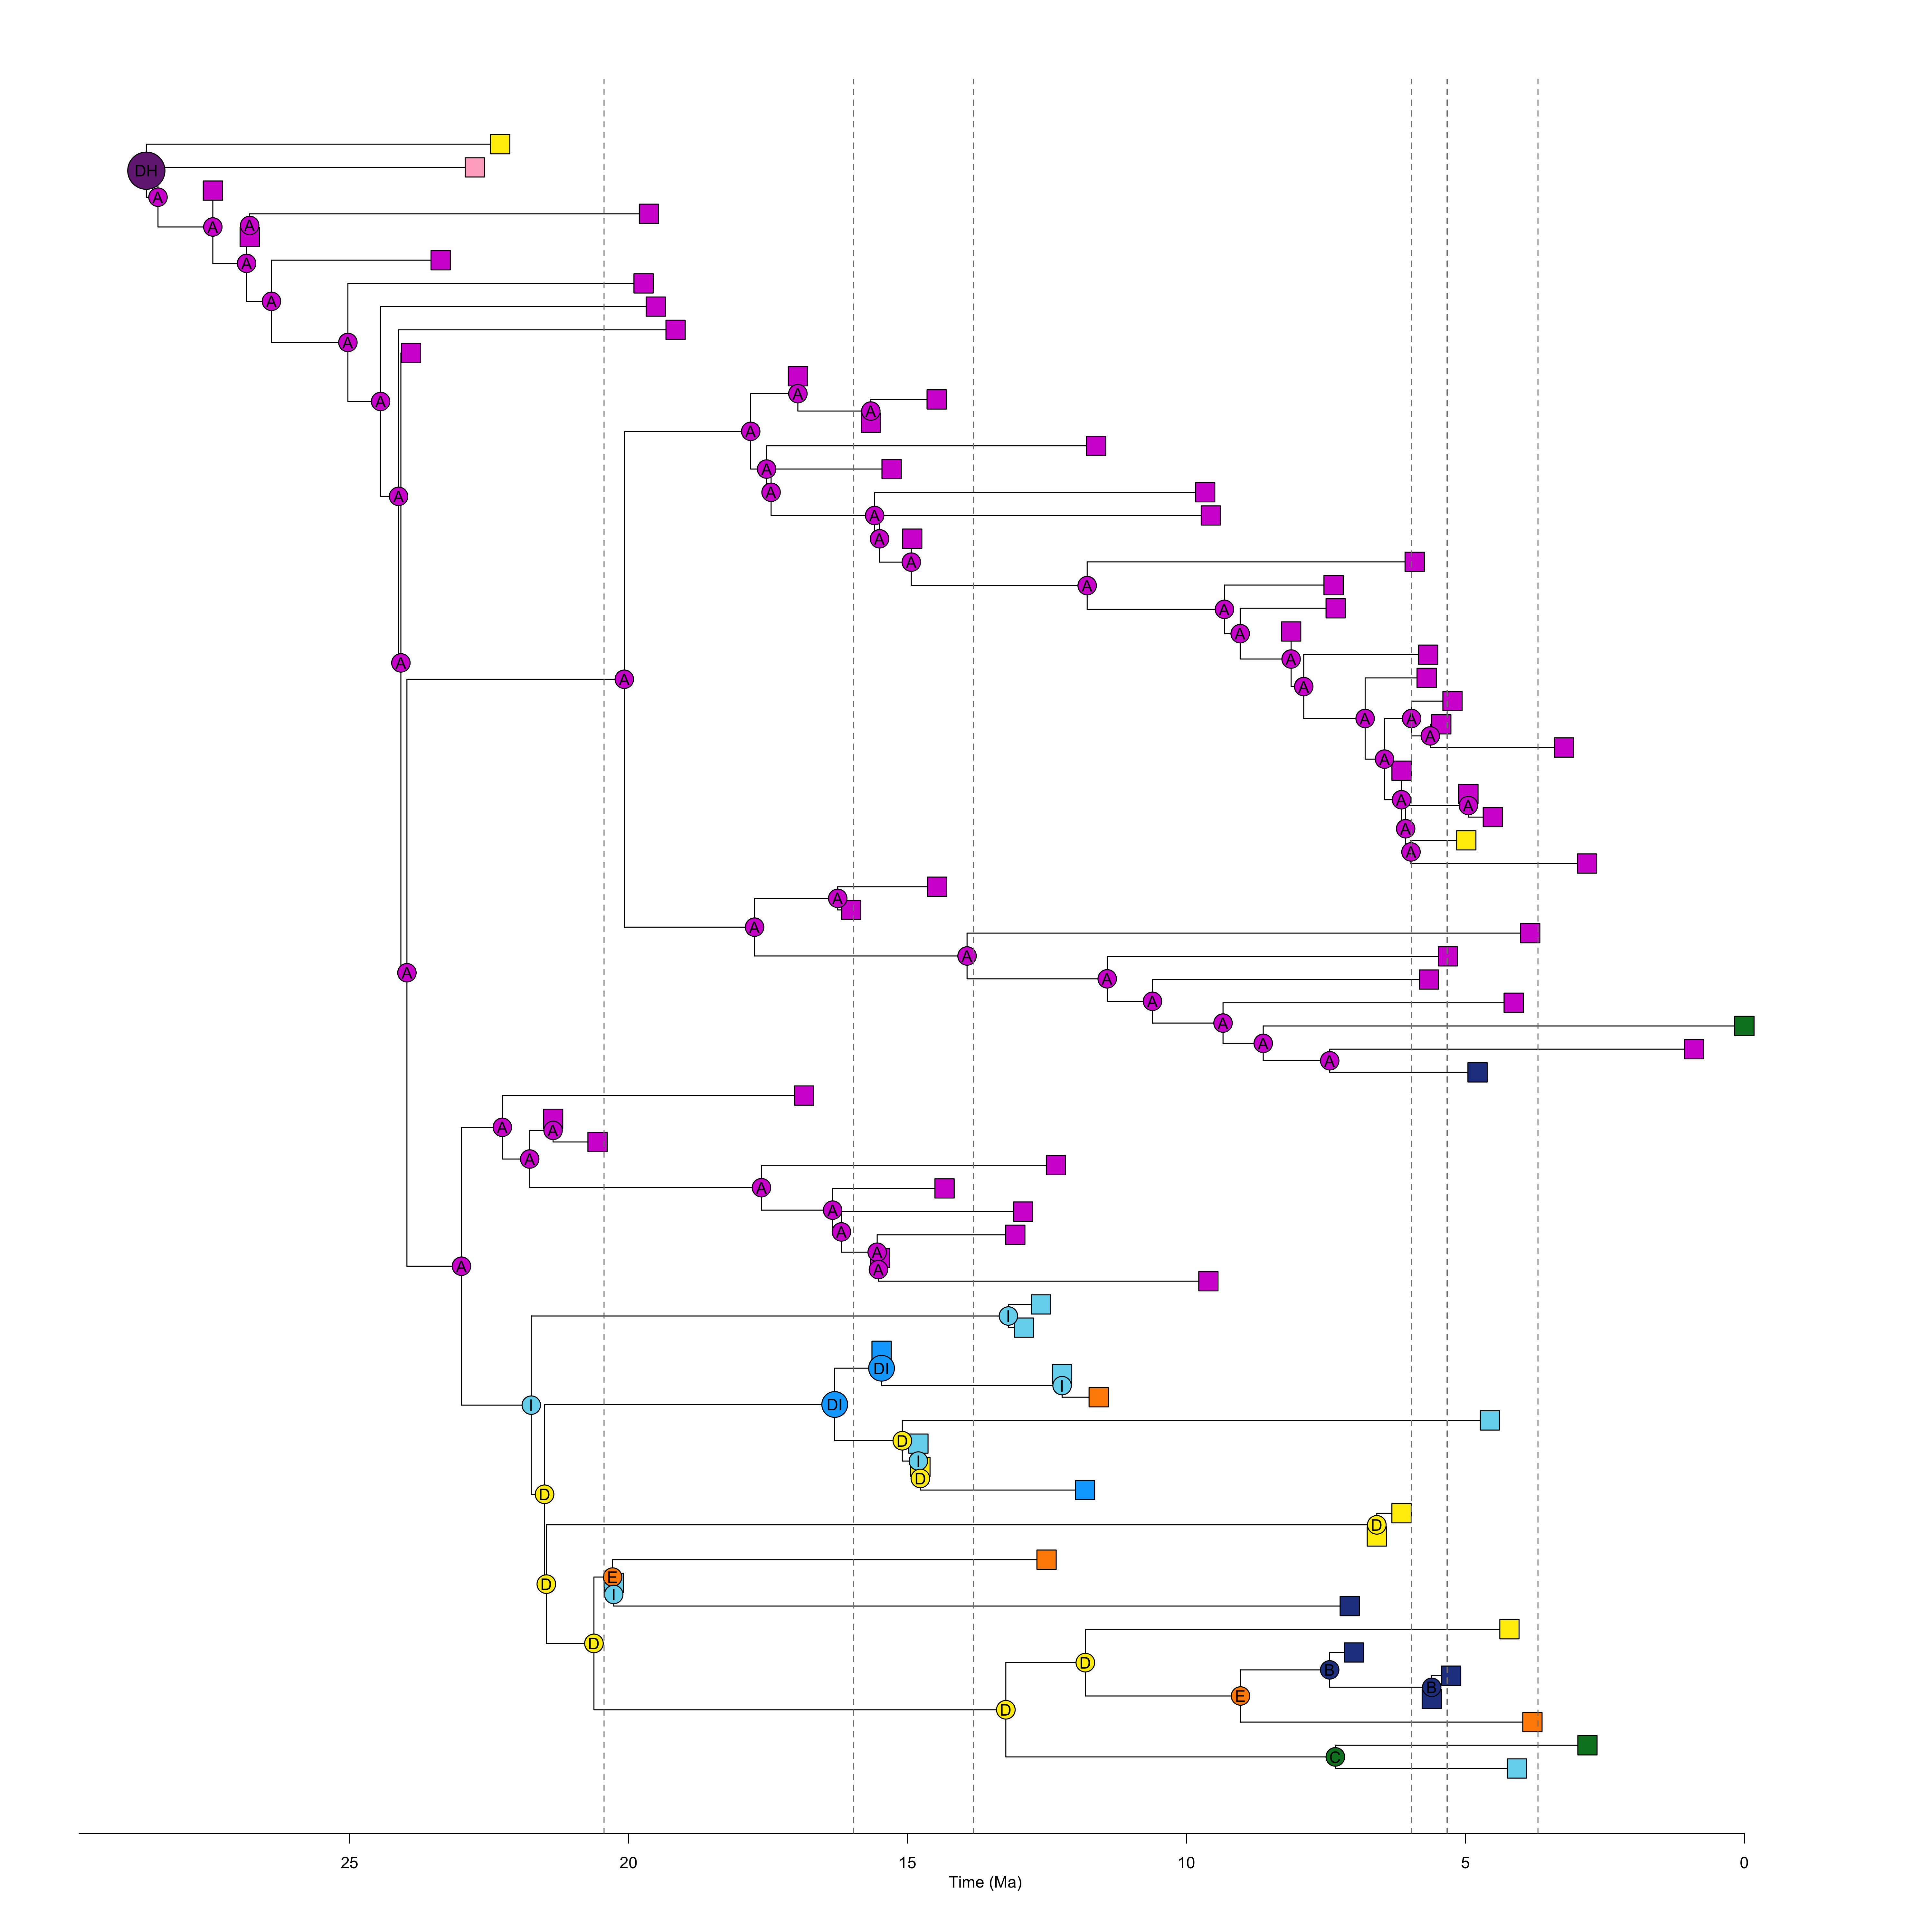
\includegraphics[width = \linewidth]{figures/fossil-pinnipeds-DECj-impossible-MLstates.png}
  \caption{Fossil pinnipeds only, DEC+J model, impossible states removed. Nodes show Maximum Likelihood states.}
  \label{fig-fossil-decj-ml}
\end{figure} 

% figure
\begin{figure}[H]
 \centering
  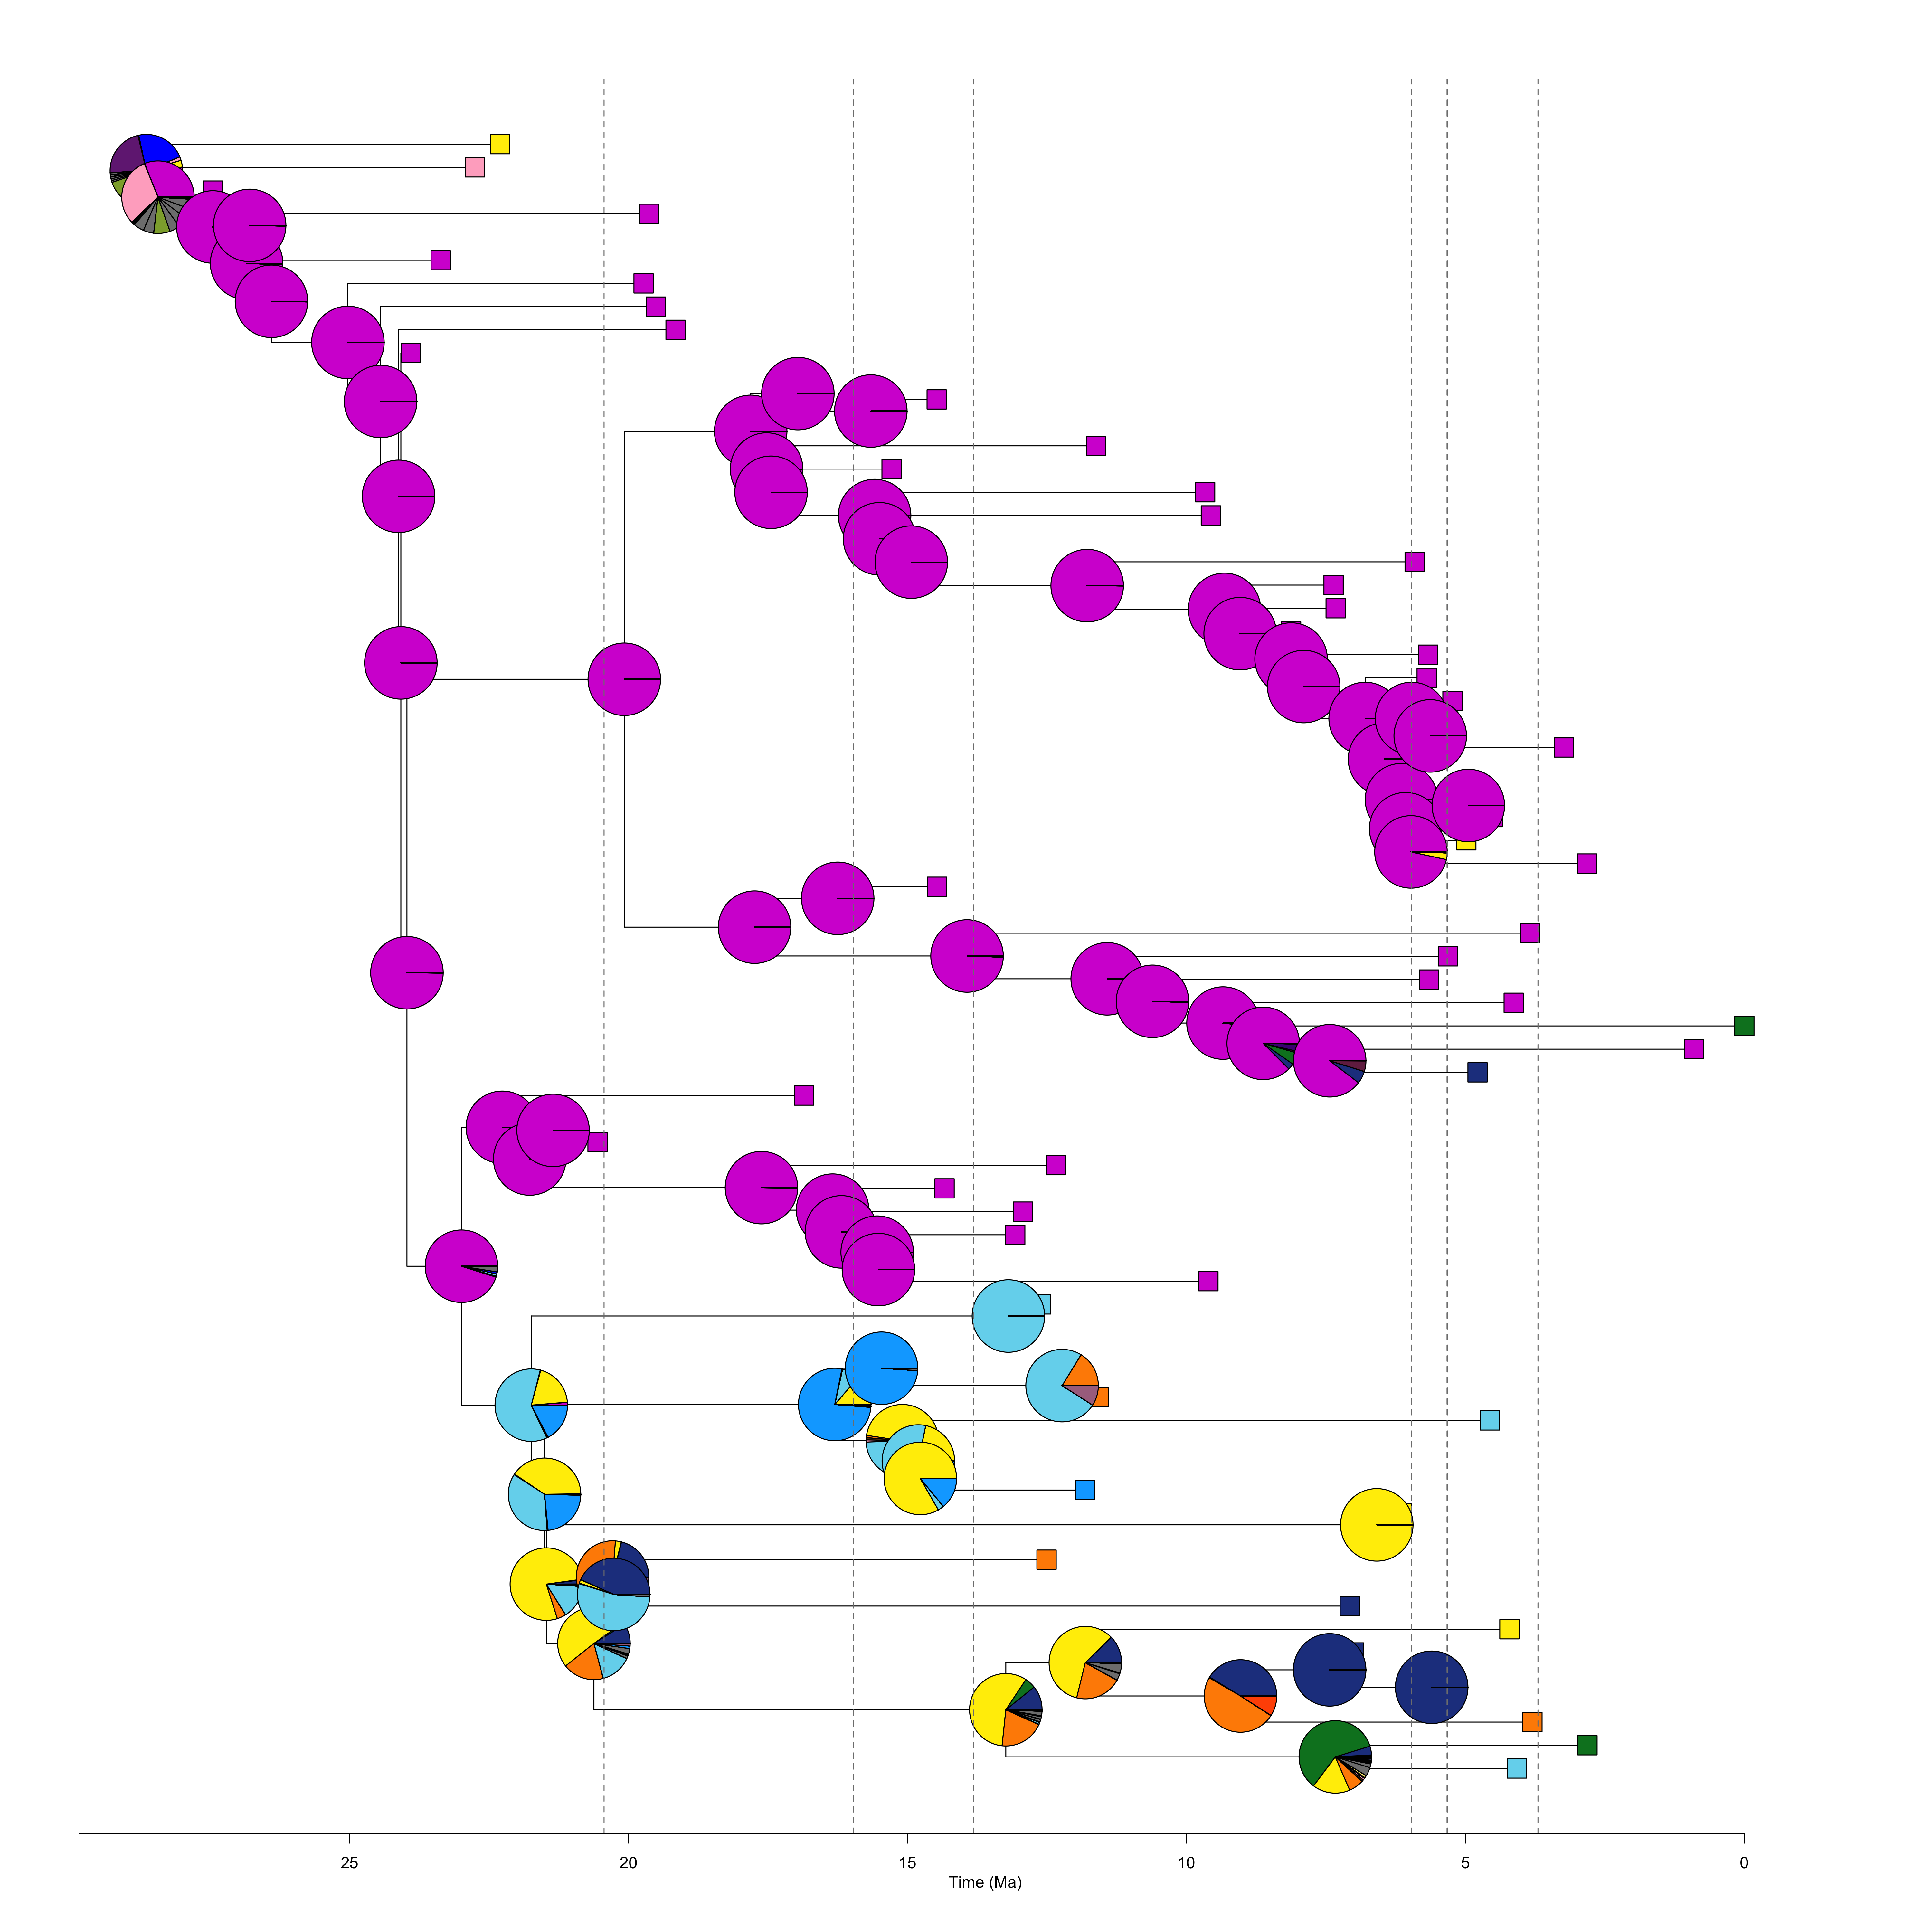
\includegraphics[width = \linewidth]{figures/fossil-pinnipeds-DECj-impossible-pies.png}
  \caption{Fossil pinnipeds only, DEC+J model, impossible states removed. Nodes show relative probabilities of each state.}
  \label{fig-fossil-decj-pie}
\end{figure} 

%-------------------------------------------------------------------------------
\subsubsection{Excluding fossil taxa from biogeographic analyses prevents robust inferences of biogeographic origins}

It has long been recognized that ancestral state estimations derived from extant species alone may be inaccurate, particularly when the tempo or mode of evolution deviates from a time-homogeneous, unbiased process \citep{omland1999assumptions,oakley2000independent,wright2015came}. A number of studies have since demonstrated that the inclusion of fossil taxa, either as terminal taxa \citep{finarelli2006ancestral,albert2009fossils,betancur2012apparent} or as prior probability distributions on node states \citep{slater2012integrating}, can overcome these deficiencies and yield more accurate estimates, particularly at deeper nodes in phylogeny. Although the recent proliferation of models of biogeographic range evolution has yielded a diverse, process-based tool-kit for estimating parameters associated with dispersal and within-region extinction, this endeavor remains one of ancestral state inference and is subject to the same biases as applications to phenotypic evolution. A number of recent studies have convincingly demonstrated that the inclusion of fossil data in historical biogeographic analyses can yield inferred ancestral ranges that are at odds with inferences derived from phylogenies of extant species only and, in some cases, suggests that entire clades may have originated in areas that they do not occur in today \citep{field2018north,gunnell2018fossil,siqueira2019historical,azevedo2021fossils,macaluso2022biogeographic}.

Pinniped systematists have increasingly converged on a view that the crown clade originated in the Northern Pacific during the Late Oligocene, and that this region was the primary theatre of diversification for stem-pinnipeds (“enaliarctines”), otarioids (sea-lions and walruses), and desmatophocids. In contrast, phocids (earless seals) originated and, at least initially, diversified in the North Atlantic. Although much of this consensus is derived from a direct reading of the rich pinniped fossil record \citep{repenning1979historical,demere2003chapter}, it is notable that such evidence is also obtainable from molecular phylogenies of extant taxa \citep{fyler2005historical,fulton2010multiple2,churchill2014colonization}. However, our analyses confirm that inference based solely on extant pinniped phylogeny is weak and, in some cases, highly ambiguous. For example, an exclusively North Pacific origin for crown pinnipeds is not recovered among the five ancestral ranges with the highest marginal likelihoods inferred under DEC or DEC+J, and a North Atlantic origin for crown Phocidae is the most likely state but with a marginal probability of just 0.1-0.15. Inference on the complete time-scaled metatree helps resolve these ambiguities and, in the case of crown Phocidae, further reveals that a North Atlantic + paratethyean or exclusively parathethyean origin is not implausible \citep[see also][]{rule2020first}. However, we also note that such biogeographic inference is obtainable from analyzing a time-scaled tree of fossil taxa alone, indicating that in pinnipeds, fossils likely contain more macroevolutionary signal than do living species. Similar results were obtained in an analysis of historical biogeography of Primates by Wisniewski et al. (\citeyear{wisniewski2022extant}) leading the authors to suggest that, all else being equal, we should prefer to conduct ancestral state inference on phylogenies of extinct taxa, rather than mega-phylogenies of extant organisms \citep[see][for a statistical justification]{ane2008analysis}. Our biogeographic inferences are consistent with this suggestion, though we note that comparison of our diversification rate estimates over the three sets of trees would argue for combining extinct and extant taxa wherever possible. 

%-------------------------------------------------------------------------------
% Refs
%----------------------------------------
\newpage
\section{Supplementary references}
 
\bibliography{pinnipeds}
\bibliographystyle{evolution}

\end{document}
